%Documentclass thesul modifée pour la page de garde : thesul-cs
\documentclass[11pt]{thesul-cs}
\usepackage[utf8]{inputenc}
\usepackage[T1]{fontenc}
\usepackage{amsmath}
\usepackage{amsfonts}

%Fancy headers
\usepackage{fancyhdr}
\pagestyle{fancy}
\fancyhf{}
\fancyhead[LE,RO]{\thepage}
\fancyhead[LO]{\rightmark}
\fancyhead[RE]{\leftmark}

%mini table of contents
\usepackage[french]{minitoc}
\usepackage{amssymb}
\usepackage{xcolor} % où xcolor selon l'installation
\usepackage{mdframed}
\usepackage{multirow} %% Pour mettre un texte sur plusieurs rangées
\usepackage{multicol} %% Pour mettre un texte sur plusieurs colonnes
\usepackage{scrextend} %Forcer la 4eme  de couverture en page pair
\usepackage{tikz}
\usepackage{graphicx}
\usepackage[absolute]{textpos} 
\usepackage{colortbl}
\usepackage{amsmath}
\usepackage{amsthm}
\usepackage{stmaryrd}
\usepackage{array}
\usepackage{url}
\usepackage[ruled,french,frenchkw,onelanguage]{algorithm2e}
%\usepackage{algorithm}
%\usepackage{algpseudocode}
\SetAlCapSkip{1em}
\SetKwInput{KwInput}{Input}
\SetKwInput{KwOutput}{Output}
\usepackage{mathtools}
\DeclareMathOperator{\sign}{sgn}
\newtheorem{propriete}{Propriété}
\newtheorem{proposition}{Proposition}
\parskip=5pt
%draft/release options
\newif\ifDraft
\newcommand\comment[1]{\ifDraft {\itshape\color{red}{#1}} \fi} %text displayed in draft mode as comments
\newcommand\draft[1]{\ifDraft #1 \fi} %text displayed in draft mode only.
\newif\ifReview
%switch between draftmode and releasemode
\ifdefined\draftmode
  \Drafttrue
  %\Reviewtrue
\fi

\ifdefined\reviewmode
  \Reviewtrue
\fi


%\Drafttrue %switch to false if you want to get the release version.
%\Draftfalse %switch to true if you want to get the draft version.
%\ifReview \usepackage[lmargin=5cm]{geometry}\fi

%def path for files


%---------------------------
% (1) Weights
%---------------------------
\newcommand\w{\omega}

%---------------------------
% (2) External inputs
%---------------------------
\newcommand\inpx{X}

%---------------------------
% (3) Contextual inputs
%---------------------------

\newcommand\inpc{\gamma}

%---------------------------
% (4) Contextual suffix
%---------------------------
\newcommand\cont{_{c}}

%---------------------------
% (5) External suffix
%---------------------------

\newcommand\ext{_{e}}

%---------------------------
% (6) Map index
%---------------------------
\newcommand\m[1]{^{({#1})}}

%---------------------------
% (7) BMU
%---------------------------

\newcommand\bmu{\Pi}

%---------------------------
% (7) Neighborhood radius
%---------------------------
\newcommand\h{h}

\DeclareMathOperator*{\argmax}{arg\,max}


%compile only a chapter

\begin{document}
\dominitoc
\ThesisTitle{Auto-organisation Décentralisée Multi-Cartes}
\ThesisDate{ ? décembre 2022}
\ThesisAuthor{Noémie Gonnier}
\ThesisUL
% Jury:
\President = {Le président &du jury}
\Rapporteurs = {Le rapporteur 1 &du laboratoire\\
Le rapporteur 2\\
Le rapporteur 3}
\Examinateurs = {L’examinateur 1\\
L’examinateur 2}
\MakeThesisTitlePage
\tableofcontents
\section*{Introduction}



\subsection*{Bio-inspiration : une thématique actuelle}

Le terme calcul désigne les procédés abstraits utilisés pour le traitement de l'information. Un système réalisants de tels procédés est alors désigné comme système de calcul. D'un point de vue abstrait, ces systèmes peuvent être biologiques comme artificiels.
Aussi le cerveau humain est un système de calcul : il transforme une multitudes de signaux physiques et chimiques provenant des capteurs du corps humain en activité électrique qui se traduisent en des actions sur l'environnement. De nombreux systèmes biologiques sont ainsi des systèmes de calcul dans le sens ou ils traitent de l'information: cellules, organismes vivants ...
La majorité des systèmes de calculs artificiels développés actuellement ont d'ailleurs commencé par une inspiration biologique. En particulier, l'intelligence artificielle et le développement des systèmes d'apprentissage automatique ont comme point de départ la question des calculs réalisés biologiquement. Le modèle de neurone artificiel utilisé en deep learning s'appuie ainsi d'abord sur un modèle biologique de neurone.
Même si la diversité des applications actuelles de l'apprentissage automatique s'est éloignée de la compréhension biologique, la question des calculs occurants dans les systèmes biologique reste une thématique de recherche dans de nombreux domaines cherchant à simuler des comportements biologiques tels que les neurosciences computationnelles. 
Inversement, les systèmes  de calcul biologiques, par leur diversité de comportements encore incompris, restent une source d'inspiration majeure pour le développement de systèmes de calcul artificiels.

Nous nous intéressons dans cette thèse à une approche bio-inspirée de la conception de systèmes de calculs, en  particulier de systèmes d'apprentissage.
Un aspect récurrant, voire de fond observé en biologique est la modularité des systèmes. On peut définir la modularité d'un système comme sa composition en sous-systèmes autonomes effectuant des tâches différentes et collaborant entre eux. Cette modularité présente des aspects de réutilisation, de robustesse à des fautes, de traitement local de l'information. En soi, tout système peut être modulaire en fonction de la représentation qu'on lui choisit~; mais il existe des similitudes dans la structure de nombreux systèmes. De nombreux systèmes biologiques sont en effet composés de nombreux modules de même structure, ayant des règles d'évolution locales,  interagissant entre eux. Dans ce cas, le comportement global du système est plus.
Certains expliquent même le coté modulaire comme une conséquence de la sélection évolutive des systèmes.

 Les neurones du cerveau en sont un exemple. Chaque neurone est construit sur le même modèle et les règles d'évolution de chaque neurone sont similaires. Dans son ensemble, le cerveau présente des comportements de calculs qui lui sont propres.
Dans ce même cerveau, à  une plus grande échelle, on peut séparer des zones fonctionnelles distinctes dans le cerveau. Chaque zone est de construction similaire, mais effectue une fonction différente.
Le cerveau n'est pas le seul système biologique présentant ce type de fonctionnemment. Ainsi, les systèmes métaboliques ou d'expression de gènes sont des exemples de systèmes aggrégeant des éléments.
Les colonies de fourmi sont constituées de milliers d'individus effectuants des actions à leur échelle et communiquant localement. Le comportement de la colonie est un système de calcul, capable de résoudre des problème d'optimisation de chemin vers une source de nourriture.
Les calculs occurrant dans ces systèmes modulaires sont appelés comportements émergeant : chaque module du systèmes effectue des calculs et actions locales, mais le comportement du tout est plus complexe que la somme de chaque partie.
Cette notion d'émergence, dont nous avons donné des exemples biologiques, a inspiré de nombreux modèles de calcul en intelligence artificielle et robotique.
Par exemple, l'intelligence d'essaim (swarm intelligence) est une direct application de ce concept à des sytèmes multi-agents qui interagissent localement avec leur environnement. 
Le jeu de la vie permet d'effectuer des calculs et de propager de l'information malgré la simplicité des règles d'évolution de chaque cellule. Enfin, les calculs rendus possibles dans les réseaux de neurones proviennent du comportement collectif des neurones et sont donc un exemple d'émergence au sein de systèmes d'apprentissage.


La modularité présente des aspects avantageux pour le calcul, voire optimaux. En témoigne les architectures de modèles artificiels, a priori pas du tout inspirés de la biologie, à des modèles biologiques existants. Une structure de réseau en petit monde est  utilisée dans des systèmes d'information, comme des bases de données, comme une structure optimisant la vitesse des échanges d'information dans le système. Or, ces strctures sont observées dans de nombreux domaines expérimentaux : biologie (exemple ?) et même dans des systèmes sociaux tels que les arbres de connaissances entre individus.

 D'un point de vue informatique, on peut définir la modularité comme la décomposition d'un système en sous-systèmes plus petits et fonctionnant indépendamment. Ces systèmes interagissent via une interface bien définie.
Plusieurs façon de construire ces sous-systèmes. Dans un cas de figure, ces composants sont conçus pour être interchangeables et réutilisables.
La modularité permet alors à un système d'être robuste à un dysfonctionnement d'un composant, sa mise à l'échelle et un faculté d'adaptation.

Un système modulaire n‘est pas forcément un système complexe.
Cependant, lorsque l'interaction des modules est diverse et non linéaire, le système mène à l'émergence de nouveaux comportements.

\subsection*{Modularité et Conception d'architectures d'apprentissage}

Les systèmes d'apprentissage existants combinent la notion de modularité et d'émergence pour former des comportements d'apprentissage plus complexes.
Les réseaux de deep learning, se sont éloignés du modèle biologique du neurone pour ajouter des règles de calculs plus informatiques comme la backpropagation. Cependant l'approche modulaire est resté une constante dans le développement des réseaux utilisés actuellements comme le modèle teacher student et les réseaux de neurones adversarials qui combinent des réseaux performant chacun une sous-tâche par rapport à l'autre.

La conception de système modulaire d'apprentissage peut passer par deux approches. D'un coté, une approche “finale” dans laquelle la finalité, l'application du système est connue. La conception du sytèmes passe alors par la décomposition de l'objectif en sous-systèmes et sous-tâches de manière à définir des modules particuliers.
L'approche inverse serait l'approche constructive, dans laquelle nous disposons de modules permettant des comportements simples de calculs et les associons entre eux pour former un système modulaire. Il est difficile de connaître à l'avance le comportement final de ce type de sytème et son étude passe donc par la simulation.
Cette approche, si elle n'est pas la plus rapide en terme de résultats applicatifs, a l'avantage d'ouvrir la porte à des comportement d'apprentissages qui peuvent être inattendus. 

Exemples d'archi modulaires d'apprentissage ? ART, Reservoir

\subsection*{Le calcul local et décentralisé, une problématique actuelle des réseaux de neurones}

Modularité et calcul local sont des problématiques liées. De nos jours, la consommation energetique grandissante des  algorithmes de traitement de l'information  

3 – Les cartes auto-organisatrices comme choix de modules

Nous avons choisi dans cette thèse de s'intéresser à cette deuxième approche~: développer un système modulaire apprenant en associant des réseaux existants connus. Nous nous intéressons spécialement aux cartes auto-organisatrices.

Si nous revenons à un aspect biologique, les cartes auto-organisatrices sont, par leur comportement un modèle simplifié des aires cérébrales. Les travaux conduits dans notre équipes ces dernières années se sont attachés à construire des architectures modulaires complètement cellulaires. Nous cherchons dans cette thèse à s'inspirer de ces travaux mais en les passant à une échelle moins cellulaire, dans un cadre de simplification du modèle. Cette simplification nous permet une recherche plus facile et moins coûteuse de nouveaux comportements d'apprentissage, tout en restant déclinable si besoin en version cellulaire.
Dans un cadre d'architecture modulaire, 


\section{Contributions et plan}

Cette thèse cherche donc, dans un cadre bio-inspiré, à construire une architecture modulaire décentralisée de cartes auto-organisatrices. L'idée de cette approche est de rechercher des nouveaux comportements d'apprentissage émergeant de l'interaction entre les modules d'une grande architecture, à l'inverse des méthodes plus ingénieures consistant à diviser une tâche connue en sous-systèmes.
Nous commencerons par présenter un état de l'art des architectures de cartes auto-organisatrices existantes afin de définir ce qu'on entend par architecture modulaire décentralisée et positionner notre modèle dans l'ensemble des modèles existants.
Nous détaillerons ensuite notre modèle d'architecture décentralisée de cartes auto-organisatrices.
Si le modèle a pour but à long terme de concevoir une architecture comportant de nombreux modules, nous avons concentré cette thèse sur l'analyse des comportements d'architecture de deux et trois cartes.
Le but de cette thèse est alors de proposer une méthodologie d'analyse de ce modèle et d'en tirer des comportements élémentaires.
Nous proposerons une méthode expérimentale et des représentations rapprochant l'architecture de cartes de modèles d'apprentissage communs au chapitre 3.
Les résultats présentés dans les chapitres 4,5,6,7 présentent le comportement du modèle CxSOM sous différents angles.
Nous analyserons plus en détail l'interface entre cartes et une recherche de BMU originale que nous utilisons.
Nous présenterons ensuite les comportements élémentaires observés sur des architectures de deux et trois cartes en une dimension, qui sont plus facile à visualiser. Nous présenterons notamment un comportement de prédiction rendu possible par le modèle.
Nous proposons au chapitre 6 des indicateurs numériques originaux d'évaluation de l'apprentissage associatif par l'architecture de cartes, dans le but d'étendre l'analyse du modèle à des architectures difficilement représentables visuellement.
Le chapitre 7 applique la méthode d'observation à des cartes en deux dimensions afin de saisir la scalabilité du modèle.

Les travaux présentés dans cette thèse ont fait l'objet de deux présentations en conférence~:
\begin{itemize}
    \item Consensus driven ...., ICONIP 2020
    \item Input prediction in SOMs, ISCMI 2021
\end{itemize}

A placer : 

Apprentissage supervisé / non supervisé définition.
Mémoire associative/traitement de séquences 


% \begin{itemize}
%     \item Apprentissage non supervisé, quantification vectorielle : définition + apprentissage développemental ? Pq c'est cool de continuer a etudier les SOM ?
%     \item Modularité et modularité dans les programmes informatiques,définition
%     \item Systèmes dynamiques complexes~: Biologique first puis exemple automates cellulaires qui sont une machine de turing, réseaux de Hopfields, machine de bolztmann: comporements de calcul comme émergeance
%     \item Systèmes d'apprentissage modulaire : des systèmes complexe.
% \end{itemize}

% \cite{Oudeyer2010OnTI} : biologie liée dans les deux sens à l'aspect computationnel.


% But : montrer comment un mécanisme de recherche de consensus entre cartes de Kohonen permet de construire des architectures apprenant des relations multimodales.
\mainmatter
\documentclass[../main]{subfiles}
\ifSubfilesClassLoaded{
    \dominitoc
    \tableofcontentsfile
}{}
\begin{document}

\graphicspath{{01-Modularite/},{./}}
%%%%%%%%%%%%%%%%%%%%%%%%%
% Intro du chapitre : Trouver un questionnement, un exemple qui parle de modularité dans les systèmes biologiques:  
% se placer dans le contexte de 
% - modularité : finalement on ne sait pas trop ce que c'est 
% - apprentissage ! 
% - réseaux de neurones
%%%%%%%%%%%%%%%%%%%%%%%%%
\chapter*{Introduction}


Le terme d’intelligence artificielle apparaît en 1956 lors d’une conférence donnée à l’université de Dartmouth, Dartmouth Summer Research Project on Artificial Intelligence. Cette conférence rassemble des chercheurs issus de différents domaines en plein essor de création comme la cybernétique, le traitement de l’information, la logique, la biologie, et veut poser les bases d’un nouveau domaine, nommé à cette occasion par les organisateurs Minsky et McCarthy: “Intelligence artificielle”. 

Ce terme générique est en fait large: on va appeler intelligence artificielle tout programme capable d’effectuer des tâches compliquées dont seuls les humains étaient initialement capables de résoudre. 
En terme d’architectures, les programmes d’intelligence artificielle peuvent être des systèmes figés à base de logique tels que les systèmes experts, ou des systèmes évolutifs. Parmi les tâches dites humaines se trouve en effet la notion d’apprentissage. La création  d’un système apprenant à partir d’entrées devient alors un enjeu à part entière de l’intelligence artificielle qu’on nommera apprentissage automatique ou en anglais machine learning.
Ces 60 dernières années ont alors vu les systèmes “intelligents” évoluer, se diversifier, pour résoudre de plus en plus de tâches jusqu’alors considérées comme humaines.

La conception de ces programmes passe par différentes sources d'inspirations, la biologie y prenant une place de premier choix.

\section*{Conception d'algorithmes d'apprentissage par modularité}

\subsection*{Définition de modularité}

La modularité en informatique se définit comme l'assemblage d'éléments séparés en une fonction globale, avec la condition qu'ajouter ou enlever un element ne modifie pas les autres éléments et influe seulement sur la fonction globale.

La majorité, voir tous les systèmes biologiques peuvent etre compris comme des systèmes modulaires. Il semble d'ailleurs que les systèmes modulaires sont privilégiés par l'évolution et des réseaux de forme similaire se retrouvent ainsi dans de nombreuses branches de la biologie: le cerveau présente des structures de réseau en petit monde que l'on retrouve dans l'organisation des ….
L'ingénieurie, sans même s'inspirer de la nature a recréé ces réseaux: les réseaux small world sont les plus efficaces pour la représentation de bases de données, ou la conception des réseaux aériens.
	
Cette notion de modularité concerne l'informatique en général: le concept peut etre appliqué au développement d'algorithmes.


\subsection*{Conception d'algorithmes d'IA}

La conception d'algorithme passe par piocher dans un ensemble de concepts et de fonctions connues, en les assemblant entre elles. 
La démarche de création d'algorithme peuvent etre ascendantes ou descendantes. 

Exemple d'algos d'IA → 
Ainsi, dans les années 1960, des premiers programmes d'intelligence artificielle repose sur des “micro mondes”, postulant qu'il est plus simple de décomposer les taches en taches plus simples afin de résoudre des comportements plus compliqués.

\subsection*{Approche ascendante vs approche descendantes}

On peut choisir deux axes de recherche pour développer un programme modulaire.
 L'approche descendante, la plus souvent utilisée, part du problème applicatif à résoudre pour le décomposer en probèmes-blocs plus simples.  et on estime que l'assemblage d'éléments exécutant ces fonctions simples nous permettrons d'effectuer la fonction complexe.
Cette démarche est très applicative. Elle est maitrisée: on connait la fonction finale, il suffit de trouver les meilleurs composants pour effectuer cette tache. Généralement, on a de bons résultats
Par contre, on ne pourra pas trouver de nouveaux paradigmes de calculs dans ce cadre: il s’agit plutot d’utiliser et d”appliquer des méthodes connues. 

Dans une démarche ascendante, il s’agit de partir de fonctions simples qu’on assemble dans l’idée d’en créer des complexes. Cette démarche est plutot exploratoire : la complexité du système fait que le seul moyen de comprendre le comportement du système ainsi créé est de le simuler. Cela peut etre vu comme un désavantage: pas possible d’avoir des équations et de choisir correctement les paramètres sans une étude des simulations. L’avantage par contre est de laisser de nombreuses opportunités ouvertes pour de nouvelles formes de calcul.
Et c’est précisément ce point qui nous amène à nous placer dans une telle démarche dans cette thèse. Nous voulons trouver de nouvelles formes de calcul pour faire de l’apprentissage. 

-----

\section*{ Modularité, systèmes complexes et emergence}

Un autre axe motivant notre reflexion sur des architectures modulaires d’apprentissage est l’observation que les systèmes modulaires sont des systèmes complexes. 

\subsection*{Système modulaire = système complexe ? }

Un système complexe est un système dont l'état est décrit par un certain nombre de variables qui évoluent de façon non linéaire. → def de qui ?
Dans la littérature, on rencontre également cette définition: système composé d'un grand nombre d'élements connectés entre eux. Cette définition rejoint la première, mais on peut noter qu'un système peut etre complexe meme à partir de 3 variables, tel que le modèle climatique de Lorentz ou le pendule triple.
 
La complexité d'un système est plutot un mode de représentation du système. La notion de systèmes complexes a été introduite dans les années 70 (Lorenz), et connait un essor depuis l'avenement des calculateur performants. 

Théorie des réseaux complexes

\subsection*{Emergence de calcul au sein d'un système complexe}

On va caractériser l'émergence de comportement dans un système complexe comme “le tout est plus que la somme des parties”, c'est à dire qu'on ne peut pas comprendre un système en le décomposant en éléments et en analysant chaque élémént individuellement: il va falloir considérer les relations entre éléments. 
La notion de systèmes complexe est étroitement liée à celle d'auto-organisation. La présence de patterns réguliers dans le comportement d'un système est directement liée à sa complexité.

\subsection*{Emergence de calcul comme moyen de conception de nouveaux algo d'IA}

D'un point de vue de création de systèmes, cela veut dire qu'on peut construire un système a partir d’éléments séparés, dont le comportement global résulte de l'interaction de ces éléments..
Le deep learning a été construit a partir du perceptron comme un assemblage de couches, dans le but de ????



\section*{ Plan de la thèse}

Dans cette thèse, nous voulons prendre une démarche constructive d'un algorithme d'apprentissage afin d'explorer de nouveaux paradigmes de calcul. Nous explorerons donc un système modulaire donc les modules sont des structures d'apprentissage existantes. Ce modèle dynamique est un système complexe, duquel pourra émerger des comportements
L'émergence de phénomènes d'auto organisation au sein des systèmes complexe nous pousse a considérer des modules possèdant déjà cette capacité d'auto-organisation: les cartes auto-organisatrices de Kohonen.
Le but de cette thèse est ainsi, dans une démarche constructive, de rechercher des nouveaux comportement d'apprentissage  à partir de cartes de Kohenen ,assemblées en architectures.
Nous nous intéressons à des modèles décentralisés, étant la clé pour construire n'importe quel type d'architecture par la suite. 
Cette démarche est difficile dans la mesure ou le comportement final d'une architecture n'est pas prédictible de prime abord. Tout l'exercice de cette thèse est alors de construire un modèle et définir des règles d'interaction, puis simuler et analyser ce modèle pour en tirer des comportements émergeants participant à l'apprentissage.
Dans cette démarche de construction, nous avons choisi des contraintes:
- Nous réalisons un système modulaire de cartes auto-organisatrices
- Cette architecture sera décentralisée: nous voulons permettre aux modules de communiquer avec n'importe lequel des autres éléments.
Le problème de cette thèse est d'étudier les comportements émergent de tels systèmes et d'étudier comment ces comportements sont un apprentissage des données.
Nous comparerons dans un premier chapitre les systèmes de cartes auto-organisatrices présentes dans la littérature et positionnerons l'architecture que nous développerons dans ce manuscrit au regard des travaux existants. Ces travaux nous permetterons de poser des hypothèses concernant le comportement qu'on peut attendre de l'architecture que nous développons. Nous présenterons ensuite le modèle CxSOM.
Nous définirons dans un chapitre la démarche expérimentale utilisée pour évaluer l'architecture de cartes et la représenter. Enfin, nous montrerons des comportements de base emergeant de la structure que nous avons développée et montrerons qu'elle a un capacité de mémoire associative. Nous présenterons egalement les limites du modèle. 
A l'issue du manuscrit, nous souhaitons que le lecteur aie une compréhension des comportements de base du modèle proposé, et aie des pistes pour l'utiliser de façon plus applicative.
\begin{figure}
    \begin{minipage}{0.49\textwidth}
        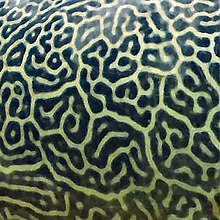
\includegraphics[width=\textwidth]{220px-Giant_Pufferfish_skin_pattern_detail}
    \end{minipage}
    \begin{minipage}{0.49\textwidth}
        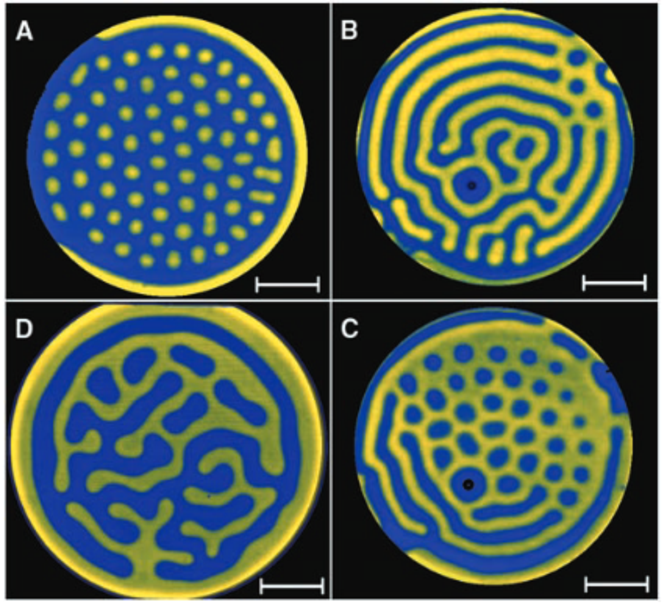
\includegraphics[width=\textwidth]{turing_pattern_chem.pdf}
    \end{minipage}
\end{figure}
\end{document}








\documentclass[../main]{subfiles}
\ifSubfilesClassLoaded{
    \dominitoc
    \tableofcontentsfile
}{}
\begin{document}
%\graphicspath{{\subfix{/02-Architectures/figures}}}
\graphicspath{{./figures},{02-Architectures/figures}}
\chapter{Architectures de cartes auto-organisatrices}
\minitoc


% Nous avons établi qu'une piste de recherche pour la construction d'algorithmes d'apprentissage passe par l'assemblage d'éléments existants comme modules d'un système, nous cherchons ainsi dans cette thèse à définir un modèle d'architecture d'apprentissage modulaire, comportant des rétroactions apportant un aspect dynamique a ce système. 
Nous nous concentrerons dans cette thèse sur la création d'architectures de cartes auto-organisatrices ou SOM (\emph{Self-Organizing Maps}) comme modules d'une architecture décentralisée.
Les cartes auto-organisatrices et notamment le modèle de Kohonen sont largement utilisées en tant qu'algorithme d'apprentissage non supervisé sur diverses applications, notamment la réduction de dimension et la visualisation de données. Cependant, peu de travaux ont exploré l'idée de les assembler en architecture comportant des rétroactions, formant ainsi un système dynamique. 
L'aspect bio-inspiré des cartes de Kohonen et la présence de motifs auto-organisés motivent pourtant cet axe d'utilisation en tant que système dynamique, motivations que nous présentons dans ce premier chapitre.

Kohonen écrivait par exemple dans son livre à propos des enjeux des cartes de Kohonen en 1995:
\begin{quote}
Un objectif à long terme de l'auto-organisation est de créer des systèmes autonomes dont les éléments se contrôlent mutuellement et apprennent les uns des autres. De tels éléments de contrôle peuvent être implémentés par des SOMs spécifiques; le problème principal est alors l'interface, en particulier la mise à l'échelle automatique des signaux d'interconnexion entre les modules et la collecte de signaux pertinents comme interface entre les modules. Nous laisserons cette idée aux recherches futures.
\cite{Kohonen1995SelfOrganizingM}
\end{quote}

% Systems of SOMs. A far-reaching goal in self-organization is to create
% autonomous systems, the parts of which control each other and learn from
% each other. Such control structures may be implemented by special SOMs;
% the main problem thereby is the interface, especially automatic scaling of
% interconnecting signals between the modules, and picking up relevant signals
% to interfaces between modules. We shall leave this idea for future research. 

L'idée de trouver de nouveaux paradigmes de calculs non conventionnels dans les SOMs à l'aide de leur assemblage en structure modulaire dynamique rejoint l'idée de Kohonen sur les systèmes autonomes. 
Il soulève la question de l'interface entre les modules, qui sera centrale dans notre construction. 
Le but de cette thèse est ainsi d'une part, de proposer un modèle de carte qui puisse être utilisée en tant que module et de définir l'interface entre modules et d'en extraire des comportements de calcul en émergeant. 
Avant toute chose, nous pouvons chercher des éléments de réponse à ces deux questions en étudiant les travaux traitant des architectures de cartes de Kohonen ou plus généralement de réseaux d'apprentissage utilisant des règles d'auto-organisation dans leur évolution. Cela nous permettra de privilégier un type d'interface au regard des travaux existants et d'émettre des hypothèses quant aux comportements attendus de l'architecture que nous proposerons.

Nous présentons ainsi dans ce chapitre le modèle général d'une carte de Kohonen et ses comportements de base; notre modèle sera ensuite décrit plus en détail au chapitre~\ref{chap:modele}.
Nous passons ensuite en revue différentes architectures de SOM proposées dans la littérature. 
Nous analyserons notamment comment la structure d'une architecture définit le type d'apprentissage effectué par un système. Nous comparerons aussi le choix du modèle d'interfaces entre cartes.
A l'issue de ce chapitre, nous aurons une vue d'ensemble organisée de différents modèles d'architectures de SOMs existantes et définirons ou se place le modèle que nous étudierons.
A la lumière des résultats des différents travaux, nous proposerons des hypothèses sur les comportements que nous pouvons attendre de notre modèle d'architecture. 
Ces hypothèses motivent les expériences conduites dans la suite de cette thèse. 

\section{Les cartes auto-organisatrices de Kohonen comme modules d'une architecture}\label{sec:som001}

Le modèle de cartes auto-organisatrice a été initialement développé par Kohonen \cite{Kohonen1982}~; nous utiliserons ainsi les termes cartes de Kohonen et SOM de façon équivalente pour désigner ce modèle initial.
De nombreux modèles dérivés ont ensuite été développés à partir de ce modèle initial, sur diverses applications.
Nous présentons dans cette section le modèle de carte de Kohonen et détaillons les possibilités qu'il offre en tant que module d'une architecture. 

\subsection{Carte de Kohonen classique}

Une carte de Kohonen est un algorithme de quantification vectorielle. Le but de la quantification vectorielle est de représenter un ensemble de données d'entrées issues d'un espace $\mathcal{D}$ en un nombre fini de vecteurs de l'espace d'entrée, les prototypes. Dans une SOM, ces prototypes sont disposés sur les n\oe{}uds d'un graphe, en général une grille en deux dimensions.
Les n\oe{}uds du graphe possèdent alors chacun un prototype et sont \emph{indexés}, par un réel ou un vecteur en deux dimensions lorsque que la carte est une grille.
Cette indexation et le format de graphe permet de définir une distance dans la carte et une notion de voisinage entre n\oe{}uds.
Nous appellerons carte de Kohonen le graphe assorti de ses prototypes.

Au début de l'apprentissage, les prototypes prennent une valeur aléatoire dans l'espace d'entrée. 
L'apprentissage est ensuite réalisé en trois étapes~:
\begin{enumerate}
\item Une entrée $\inpx$ est présentée à la carte.
\item Le n\oe{}ud ayant le prototype le plus proche de $\inpx$ selon une distance $d$ est choisie comme \emph{Best Matching Unit} (BMU) de la carte. Son index est noté $\bmu$. La distance $d$ généralement utilisée est la distance euclidienne.
\item Le prototype de la BMU est déplacé vers l'entrée $\inpx$, ainsi que les prototypes des n\oe{}uds voisins de $\bmu$ dans un voisinage défini à l'avance. On peut interpréter cette étape comme le déplacement d'une zone de la carte centrée en $\bmu$. Des exemples de voisinages sont ainsi indiquées en figure \ref{fig:topo}. Ce voisinage est défini par une fonction de voisinage dans l'algorithme qui dépend de la distance d'un n\oe{}ud au BMU et associe à chaque n\oe{}ud un coefficient multiplicatif pour la mise à jour des poids. Cette fonction est maximale à la position du BMU et décroissante autour de cette position. Il s'agira par exemple d'une fonction rectangulaire, triangle ou gaussienne.
\end{enumerate}

L'algorithme de Kohonen repose donc à la fois sur un mécanisme de compétition, avec la sélection de la BMU de la carte et un processus de coopération avec le déplacement des unités voisines de la BMU.
Toutes les données d'entrées sont tirées dans un même espace $\mathcal{D}$. L'utilisation de distances est la version originale de l'algorithme de Kohonen; elle est remplacée dans de nombreux modèles de cartes par le calcul d'une fonction d'activité liant les poids des n\oe{}uds et les entrées. 


Le processus de mise à jour des poids d'une carte de Kohonen se traduit visuellement par un dépliement de la carte dans l'espace d'entrée. On parlera donc de \emph{dépliement} d'une carte lorsque qu'on parle d'apprentissage. Ce dépliement est représenté en figures \ref{fig:som2d} et \ref{fig:som1d} pour des exemples de cartes en une et deux dimensions, se dépliant sur des données en deux dimensions. On observe d'ailleurs que les valeurs des poids à l'issue de l'apprentissage correspondent aux centres des cellules de Voronoï de l'espace d'entrée.
A la fin de l'apprentissage, la carte conserve la structure topologique des entrées:
\begin{itemize}
\item Elle conserve les distances~: deux prototypes ayant une distance proche dans la carte seront également proches selon la distance définie dans l'espace d'entrée. On observe donc une continuité des valeurs des poids au sein de la carte.
\item Elle conserve les densités. Une zone dense de $\mathcal{D}$ aura plus d'unités correspondant à cette zone de valeurs dans la carte qu'une zone moins dense.
\end{itemize}
La figure \ref{fig:SOM} présente par exemple le dépliement d'une carte sur des imagettes MNIST.
Par son aspect ordonné, une carte est une représentation en faible dimension d'un espace d'entrée de grande dimension. 

%Les cartes de Kohonen sont souvent utilisées en pratique pour visualiser des données de grande dimension et faire du \emph{clustering}. 

% La carte de Kohonen est d'inspiration biologique. Le but premier de Kohonen était de développer un modèle informatique inspiré de l'organisation spatiale des neurones dans le cortex humain, dont un exemple est présenté en figure~\ref{fig:v1}. Il s'est notamment inspiré de l'organisation du cortex en colonnes corticales, ensemble de neurones réagissant à un même stimulus.

% \draft{
% (Kohonen book 1995)
% In an attempt to implement a learning principle that would
% work reliably in practice, effectively creating globally ordered maps of various
% sensory features onto a layered neural network, this author formalized the
% self-organizing process in 1981 and 1982 into an algorithmic form that is
% now being called the Self-Organizing (Feature) Map (SOM) [2.27 -29J. In the
% pure form, the SOM defines an "elastic net" of points (parameter, reference,
% or codebook vectors) that are fitted to the input signal space to approximate
% its density function in an ordered way. The main applications of the SOM
% are thus in the visualization of complex data in a two-dimensional display,
% and creation of abstractions like in many clustering techniques.

% Motivations de Kohonen: capacité des régions du cerveau à s'auto organiser. Note que certes il doit y avoir un prédetermination génétique, mais qu'on observe une réorganisation des mapping lors de déficiences par ex. 

% find abstract self-
% organizing processes in which maps resembling the brain maps are formed,
% whereas it is of less interest whether the maps are formed by evolution, post-
% natal growth, or learning.

% }

\begin{figure}
\centering
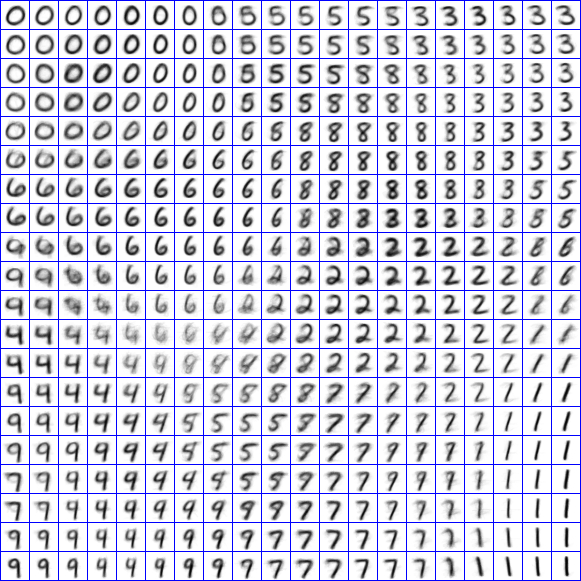
\includegraphics[width=0.5\textwidth]{digits.jpg}
\caption{Représentation de la base de données MNIST, images de chiffres écrits à main levées, par une SOM en deux dimensions. Une continuité est observée dans la forme des images lorsqu'on se déplace dans la carte~: le $0$ se transforme en $6$, etc.}
\label{fig:SOM}
\end{figure}

\subsection{Aspect topologique de la carte de Kohonen}

La carte de Kohonen se distingue d'autres algorithmes de quantification vectorielle par la topologie introduite par la carte dans l'ensemble des prototypes. Cette topologie dépend du voisinage utilisé par l'algorithme et de la dimension du support de la carte.
La plupart des implémentations de SOMs de la littérature utilisent comme support une grille en deux dimensions. L'indexation des n\oe{}uds est alors un ensemble de positions 2D.

En théorie, les cartes peuvent être une dimension (ligne), deux dimensions (grilles), ou de dimensions plus grandes. Les cartes peuvent aussi être des graphes de forme plus variable. En pratique, les grilles deux dimensions sont les plus couramment utilisées. Elles permettent d'effectuer une réduction de dimension, tout en étant facile à visualiser sur un écran. Les cartes de dimensions supérieures sont très rarement utilisées dans la littérature. Le coût de l'algorithme d'apprentissage dépend en effet du nombre de neurones, et celui-ci augmente exponentiellement lorsqu'on augmente la dimension d'une carte de Kohonen. Les calculs deviennent alors rapidement coûteux.
Les cartes une dimension sont quant à elles limitées en termes de représentation des données et sont donc rarement utilisées en pratique. Cependant, elles se prêtent mieux à la représentation graphique que les cartes 2D.
%Les calculs et l'organisation générés par l'algorithme de Kohonen sont assez complexes avec des cartes en une dimension. 
Les travaux conduits en \cite{cottrell_theoretical_2016,fort_soms_2006} apportent par exemple une formalisation mathématique de l'algorithme de Kohonen et prouvent la convergence de cartes une dimension. Les auteurs se heurtent cependant à la preuve de convergence pour des cartes en deux dimensions. Donc, les processus intervenant dans des cartes 1D sont déjà mathématiquement difficiles à formaliser, difficulté qui augmente fortement avec les dimensions.
L'étude des cartes 1D a ainsi l'intérêt d'envisager un modèle simplifié dans le cadre de développement d'un nouveau modèle de SOM, ce que nous chercherons à faire dans cette thèse, avant de proposer une extension aux cartes 2D.

Les cartes de forme autre que des grilles 1D ou 2D sont moins couramment utilisées, mais peuvent avoir des avantages. Ainsi, des cartes structurées en arbre telles que développées en~\cite{koikkalainen_self-organizing_1990} permettant une recherche de BMU structurée. Certains modèles construisent une carte de Kohonen en ajoutant des n\oe{}uds au fur et à mesure de l'apprentissage, générant une carte de Kohonen sous forme d'un graphe construit par l'algorithme, par exemple en~\cite{alahakoon_dynamic_2000, yamaguchi_adaptive_2010}.

\begin{figure}
\centering
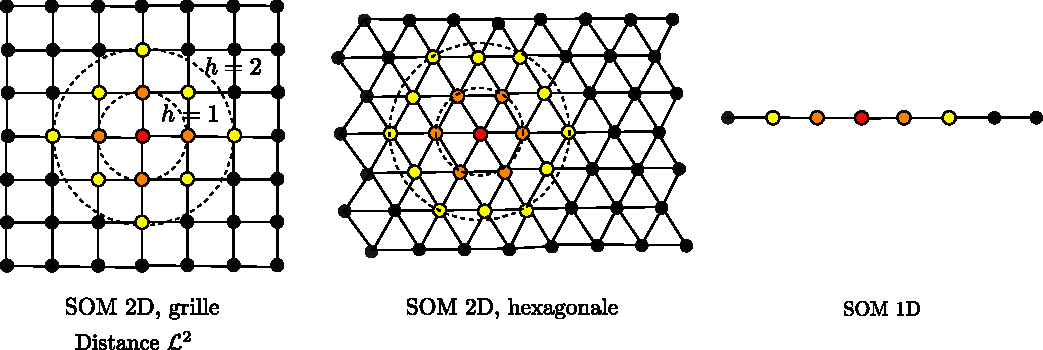
\includegraphics[width=0.8\textwidth]{soms_topologies}
\caption{Exemples de connexions dans le graphe support d'une SOM. Deux n\oe{}uds connectés sont ici à une distance de une unité dans la carte.
Les SOM en deux dimensions sont les plus communément utilisées dans la littérature, sous forme d'une grille ou d'une grille hexagonale. Les SOM une dimension sont également utilisées. \label{fig:topo}}

\end{figure}

\begin{figure}
\centering
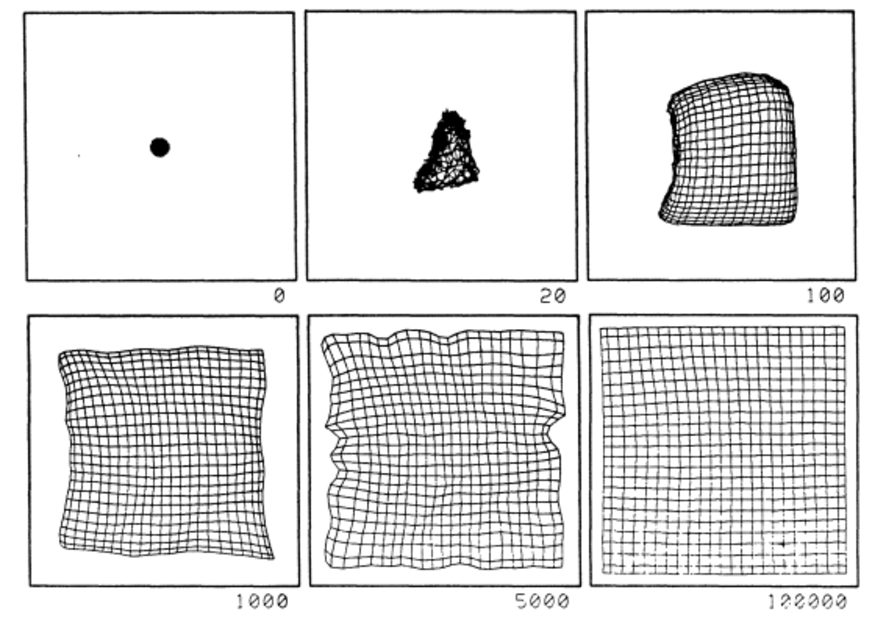
\includegraphics[width=0.7\textwidth]{som2d}
\caption{Dépliement d'une SOM 2D sur des données dans le plan $[0,1]^2$, tiré de~\cite{Kohonen1995SelfOrganizingM} \label{fig:som2d}}

\end{figure}

\begin{figure}
\centering
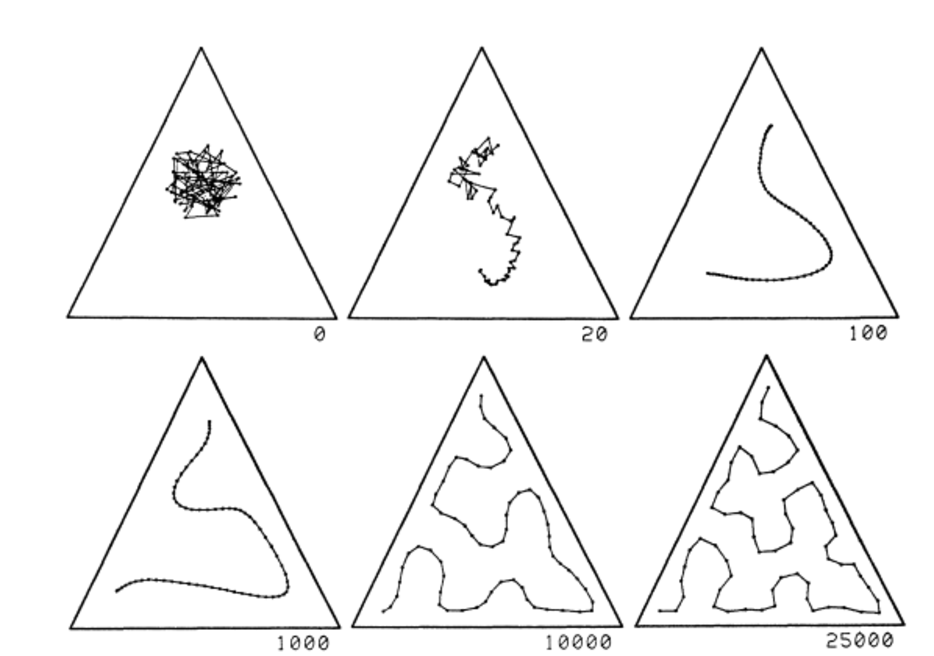
\includegraphics[width=0.7\textwidth]{som1d}
\caption{Dépliement d'une SOM 1D sur des données dans un triangle 2D, tiré de~\cite{Kohonen1995SelfOrganizingM}\label{fig:som1d}}

\end{figure}


\subsection{Inspiration biologique}

% Nous pensons ainsi que les cartes auto-organisatrices sont de bonnes candidates en tant que modules d'une architecture.
% Nous passerons en revue les modèles d'architecture existant en section suivante.
% Avant cela, il est intéressant de s'interroger sur les motivations et les intuitions motivant l'utilisation d'une carte de Kohonen en tant que module d'une architecture.

Le développement des cartes auto-organisatrices par Kohonen est initiallement inspiré par les cartes topologiques observées dans les aires du cerveau. 
Le cerveau est cartographié en \emph{aires corticales} distinctes selon la fonction principale présumée de la zone du cortex correspondante.
Le découpage fonctionnel du cerveau fait apparaître des grandes catégories d'aires corticales. Certaines aires sont dites sensorielles, car elles reçoivent des entrées sensorielles via le thalamus. Certaines aires sont dites motrices et reliées aux muscles, via des structures sous corticales et permettent ainsi un contrôle moteur.
Enfin, des aires sont identifiées comme traitant des informations venant de plusieurs autres aires.
De nombreux travaux montrent la présence de cartes topologiquement ordonnées dans différentes aires du cortex cérébral: les neurones proches dans le substrat cortical réagissent à des stimuli proches. 
Un exemple est ainsi celui du cortex visuel V1, représenté en figure~\ref{fig:v1}. 
L'aire associée à l'audition présente aussi une organisation topographique \cite{Reale1980TonotopicOI}, ainsi que de nombreuses autres aires, directement sensorielles ou plus abstraites \cite{Kohonen1995SelfOrganizingM}. 
Une carte de Kohonen ne doit cependant pas être considérée comme une modélisation biologiquement plausible d'une aire du cortex cérébral, mais plutôt comme une adaptation au niveau computationnel d'un concept biologique, ici le concept d'organisation topologiquement correcte dans les cortex sensoriels, tel que le cortex visuel ou auditif.

\begin{figure}
\centering
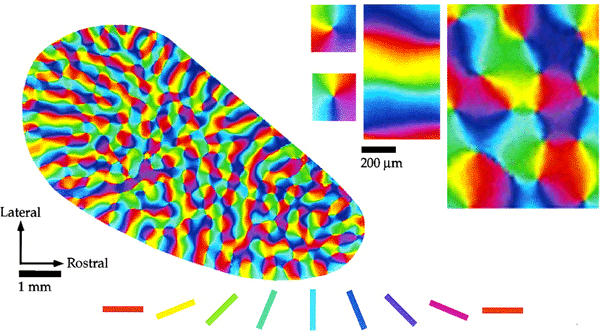
\includegraphics[width=0.6\textwidth]{v1.jpg}
\caption{Représentation des réponses du cortex visuel V1 à un stimulus visuel (bâtonnets d'orientations spatiales différentes). Les neurones répondant à une certaine orientation sont affichés de la même couleur. On observe une continuité entre les neurones proches dans le cortex et l'orientation à laquelle ils répondent. Cette propriété d'organisation est l'inspiration biologique des cartes de Kohonen.}
\label{fig:v1}
\end{figure}


Les aires du cerveau sont connectées entre elles. Notons que cette connectivité du cerveau peut-être étudiée de plusieurs points de vue~: d'un point de vue structurel, en se basant sur des éléments anatomiques ou fonctionnel.
Dans le cas fonctionnel, la connexion de deux aires est déduite de l'existence de dépendances statistiques entre l'activation des neurones des deux aires, observées par éléctroencéphalographie ou IRM fonctionnelle. Il faut noter cependant que ces observations traduisent une relation statistique et pas forcément une relation de cause à effet. 
La modélisation de la connectivité physique de ces aires à partir des observations reste donc l'objet de différentes théories cherchant à reproduire ces corrélations. 
Dans tous les cas, la présence d'aires distinctes communicantes fait l'objet d'un consensus.
Les modèles de base les plus communs pour cette communication entre neurones sont la zone de convergence-divergence de Damasio (CDZ) \cite{damasio_time-locked_1989}, et le modèle de boucles de rée-ntrées de Edelmann \cite{Edelman1982GroupSA}.
La zone de convergence divergence suggère que certaines aires corticales servent d'aires associatives pour associer d'autres zones corticales prenant des modalités sensorielles en entrée. Ces aires associatives assemblent les signaux en provenance des zones sensorielles et les propagent vers d'autres zones. 
La théorie de la ré-entrée postule quant à elle des connexions directes et réciproques entre les neurones de différentes zones sensorielles ou non. Ces connexions sont à l'origine de la coactivation de neurones dans différentes cartes.
% Un tel traitement de l'information permettrait ainsi d'expliquer l'effet ventriloque \cite{Bonath2007NeuralBO}. Lors de cet effet, une activité apparaît dans les cortices visuel et auditif pour les neurones sensibles à l'emplacement exact de la source des stimuli dans chacune des modalités. Après quelques millisecondes, correspondant au temps de trajet de l'aire visuelle à l'aire auditive via les aires associatives, on observe une activité auditive pour les neurones sensibles à l'emplacement spatial de la source du stimulus visuel.

% Le modèle classique du cerveau proposé dans les années 60 [Jones and Powell, 1970] modélise le cortex comme un système de traitement hiérarchique et séquentiel de l'information. Les différents flux sensoriels seraient traités par des aires corticales dédiées, et leur mise en relation dans des aires associatives ui s'occuperaient de tâches de plus haut niveau. 
% Ces flux d'informations circuleraient dans les deux sens: une aire de plus haut niveau recoit des flux d'information montant d'une aire sensorielle, et l'aire sensorielle reçoit des flux d'information descendant des aires associatives. Ce modèle de connexion est par exemple modélisé en \cite{damasio_time-locked_1989}, travaux dans lesquels les zones associatives sont désignées par "zones de convergence-divergence".

% Cette vision hiérarchique historique du traitement cortical de l'information est cependant remise en question par d'autres observations biologiques. Ainsi, \cite{eckert_cross-modal_2008} suggère l'existence de connexions directes entre les aires sensorielles visuelles et auditives. Des théories telles que la réentrée suggère l'existence de neurones multimodaux au sein d'une aire sensorielle. Anatomiquement, de nombreuses connexions, dites bas niveau, entre les aires corticales dédiées au traitement d'une modalité sensorielles ont été mises en évidence chez différentes espèces, pour des aires à différents niveaux hiérarchiques de traitement de l'information(voir [Calvert and Thesen, 2004b, Cappe et al., 2009, Cappe and Barone, 2005, Foxe and Schroeder, 2005, Kayser and Logothetis, 2007, Macaluso, 2006, Schroeder et al., 2003, Schroeder and Foxe, 2005]).
La carte de Kohonen implémentant des concepts computationnels qu'on retrouve en biologie au niveau de l'aire cérébrale, nous pouvons chercher à pousser l'inspiration biologique d'une carte de Kohonen au niveau des connexions entre les aires cérébrales, se transcrivant par des connexions entre plusieurs cartes de Kohonen.
De la même façon qu'une carte n'est pas un modèle biologique, il s'agit plutôt de développer un modèle computationnel qui ne soit pas biologiquement plausible au niveau neuronal, mais dont la structure du traitement de l'information est inspirée de celle du cerveau, ici la présence de plusieurs aires connectées entre elles, modélisées par l'utilisation de plusieurs cartes de Kohonen en architecture.

\section{Architectures de cartes auto-organisatrices}

Plusieurs travaux dans la littérature informatique autour des SOMs cherchent ainsi à construire des architectures de cartes auto-organisatrices. Cette section passe en revue certains modèles.
Nous abordons ces modèles d'un point de vue structurel en s'intéressant notamment à comment s'effectue l'interface entre les cartes dans chacun des modèles. A la lecture des modèles existants, nous avons pu différencier deux grandes classes d'architectures de cartes~: les architectures \emph{hiérarchiques feed-forward} et  les architectures \emph{non-hiérarchiques}, qui peuvent elles-mêmes être \emph{centralisées} ou \emph{décentralisées}.
Nous détaillerons dans cette section ce qu'on appelle architecture hiérarchique et non-hiérarchique et analyserons les comportements d'apprentissage émergeant des différentes structures. L'analyse de ces modèles nous permet de nous situer dans la littérature et d'émettre des hypothèses concernant les comportements attendus d'un tel modèle et ainsi de guider les expériences que nous effectuerons.

\subsection{Architectures hiérarchiques de cartes}

Dès les débuts du développement des SOMs dans les années 1980 des travaux proposent des architectures à base de cartes auto-organisatrices. Ces premiers travaux font apparaître des architectures qu'on peut qualifier de hiérarchiques.
Toutes les architectures hiérarchiques comportent plusieurs cartes, et ont comme point commun qu'il est possible de définir des \emph{niveaux} dans l'architecture, comprenant une ou plusieurs cartes. L'apprentissage des cartes dans toutes ces architectures est effectuée niveau par niveau. Nous les qualifierons ainsi d'architecture \emph{feed-forward}. 

\subsubsection{Architectures hiérarchiques sélectives}

Certains travaux s'appuient sur des architectures hiérarchiques qualifiera de "sélective", dont le principe général est illustrée en figure \ref{fig:hsom_selective}. Toutes les architectures présentées peuvent être séparées en niveaux, dont un niveau d'entrée, un niveau de sortie et des niveaux intermédiaires.
Le premier niveau d'une telle architecture est une carte classique, prenant des données en entrée. 
Après apprentissage du premier niveau, le second niveau est composé de plusieurs cartes.
L'activation ou le BMU de la carte du premier niveau à une entrée permet de sélectionner une carte du deuxième, à laquelle sera présentée cette même entrée. 
Chacune des cartes du deuxième niveau est alors entrainée sur un sous-ensemble des données d'entrée. Pour chaque entrée, la carte à mettre à jour est sélectionnée en fonction de la réponse du premier niveau à l'entrée, d'où
qualification de sélective pour le mode de communications entre cartes~; le premier niveau n'est plus mis à jour lors de cette phase.
Le processus est répété ainsi de suite si besoin sur d'autres niveaux. Les niveaux supérieurs ont alors plus de cartes que les niveaux inférieurs.
Ce procédé est retrouvé dans \cite{barbalho_hierarchical_2001,suganthan_pattern_2001}
\cite{miikkulainen_script_1992} pour de la classification de phrases, \cite{dittenbach_growing_2000,ordonez_hierarchical_2010}, ou encore en \cite{zhao_stacked_2015} pour de la détection d'arrière-plan.

La façon de sélectionner une carte d'un niveau diffèrent ensuite en fonction des travaux.
\cite{barbalho_hierarchical_2001} utilisent la position du BMU calculée au premier niveau pour choisir la carte du second niveau à utiliser. L'architecture utilisée en \cite{zhao_stacked_2015} utilise plusieurs couches de cartes pour du traitement de séquence. Cette fois, le processus de sélection s'opère en choisissant ou non de transférer l'entrée courante au niveau suivant, en s'appuyant sur la distance moyenne de la réponse des cartes à l'entrée.

\begin{figure}
    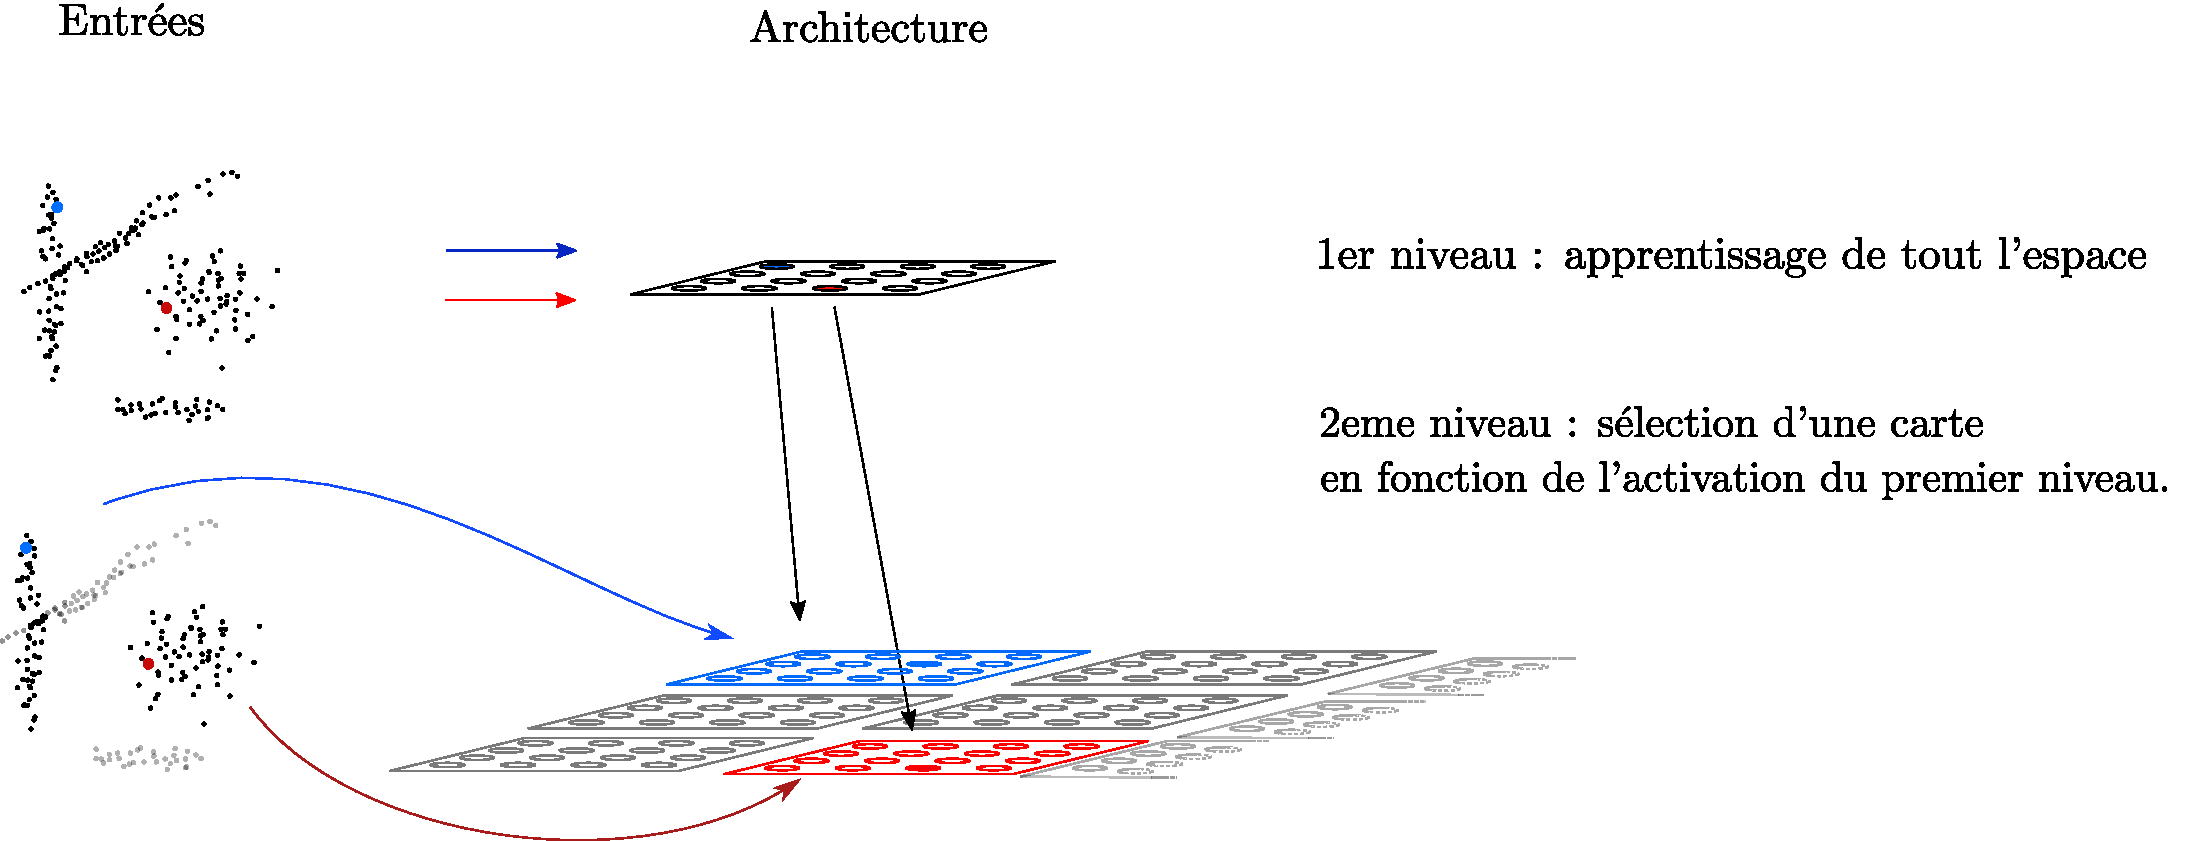
\includegraphics[width=\textwidth]{HSOM_selective.pdf}
    \caption{Exemple d'architecture hiérarchique sélective. La carte du premier niveau est entraînée sur tout l'espace d'entrée. Après apprentissage, la carte permet de filtrer les entrées pour les renvoyer vers une carte du niveau suivant. Dans cet exemple, la position du BMU de la carte du niveau 1 permet de sélectionner une carte du niveau 2, comme c'est le cas en \cite{barbalho_hierarchical_2001}. 
    L'entrée permet d'entraîner une carte du deuxième niveau. Chacune des cartes du niveau 2 apprend alors sur un sous-espace d'entrée.\label{fig:hsom_selective}}
\end{figure}

Dans ce type d'architecture, c'est un processus extérieur aux cartes qui permet de sélectionner la carte du niveau suivant. Les connexions permettent à chacune des cartes de se spécialiser sur une partie de l'espace d'entrée.
Face à ces structures sélectives, on peut imaginer une structure présentant une interface entre cartes qui soit une transmission d'une représentation des données générée par une carte.

\subsubsection{Architectures hiérarchiques par transmission de représentation intermédiaire}

Contrairement aux architectures par sélection, la deuxième couche de carte ne prend plus comme entrée un élément de l'espace d'entrée de l'architecture, mais travaille sur des éléments des cartes des couches précédentes, tels que la position, le poids du BMU ou une intensité d'activité neuronale. 
Ces éléments sont une représentation latente intermédiaire de l'entrée, transmise à la couche supérieure. Les niveaux supérieurs de ce type d'architecture ont moins de cartes que les premiers niveaux et peuvent être considérés comme traitant l'information à un niveau plus abstrait que les cartes du premier niveau.
L'architecture  HSOM \cite{lampinen_clustering_1992} proposée dès 1992 est composée de deux cartes~: une carte apprenant sur des entrées $x$, et une carte prenant comme entrée la position du BMU de la première carte~; cette architecture est illustrée en figure~\ref{fig:hsom}. La position du BMU est ici la représentation intermédiaire transmise aux cartes du niveau suivant.
Comme les cartes s'organisent de façon à conserver les distances dans l'espace d'entrée au sein de la carte, deux éléments faisant partie d'un même groupe de données (cluster) auront des BMUs proches dans la première carte~; par conséquent, leurs BMU dans la seconde carte le seront également. 
Les auteurs notent que l'architecture HSOM permet de bien détecter des clusters de données, avec une séparation des clusters un peu meilleure qu'une SOM classique. La présence de la carte intermédiaire change un peu la façon de séparer les données par rapport à une SOM classique~; les auteurs notent une meilleure séparation des clusters dans HSOM, mais une moins bonne quantification vectorielle au sein d'un cluster. Le fait d'utiliser deux SOMs permet d'extraire une représentation un peu différente que celle extraite par une SOM classique.
Par le choix de la position du BMU comme vecteur de transmission d'information, les auteurs de HSOM exploitent totalement l'aspect topologique qu'offrent les cartes de Kohonen. D'autres travaux par la suite implémentent des modèles similaires transmettant la position du BMU entre cartes, sur des architectures comportant plus de cartes que HSOM, tel que \cite{hagenauer_hierarchical_2013}.
Comme dans les modèles sélectifs, la représentation intermédiaire considérée peut également être les poids des BMUs du premier niveau, comme c'est le cas en \cite{wang_comparisonal_2007, gunes_kayacik_hierarchical_2007}.

On observe un regain de publications sur les architectures de cartes auto-organisatrices après 2015, cette fois sous la terminologie de \emph{Deep SOM}.
La plupart des travaux portant sur ces \emph{Deep SOM} implémentent des cartes hiérarchiques assez similaires aux travaux mentionnés précédemment. 
Mais cette fois, ces travaux s'inspirent des réseaux de neurones profonds (\emph{Deep Learning}), ayant connu leur essor cette même année avec les réseaux convolutionnels permettant l'apprentissage supervisé d'images de façon inégalée \cite{lecun_deep_2015}.
Par analogie avec les réseaux convolutionnels, les Deep SOM s'intéressent souvent à l'apprentissage d'images par des SOMs. Ainsi \cite{Liu2015DeepSM,hankins_somnet_2018,wickramasinghe_deep_2019,aly_deep_2020,sakkari_convolutional_2020,dozono_convolutional_2016,nawaratne_hierarchical_2020-1,mici_self-organizing_2018} et sont présentés comme des "SOMs convolutionnelles". La façon d'associer ces cartes en architectures rappellent cependant les SOMs hiérarchiques.

Par exemple, le modèle introduit en \cite{Liu2015DeepSM} est illustré en figure~\ref{fig:dsom} et s'inspire des réseaux de neurones convolutionnels.
Le but d'une telle architecture est de classifier des images. Une fenêtre est déplacée sur l'image d'entrée et chaque imagette nourrit alors une carte d'une première couche, donnant $N_{maps}  \times N_{maps}$ positions de BMU $j_{p,q}$. Ces positions représentées comme des valeurs en une dimension sont assemblées en une image intermédiaire, chaque pixel prenant la valeur du BMU de la carte correspondante. Une deuxième étape de fenêtrage peut alors être appliquée sur cette image, et ainsi de suite. La dernière couche du réseau est composée d'une SOM qui effectue alors la tache de classification de l'image intermédiaire, vue comme une représentation abstraite  de l'entrée.
L'interface entre les couches "convolutionnelles" est créée à partir des BMUs des SOMs: l'architecture DSOM s'inscrit ainsi directement dans la lignée de HSOM, à la différence qu'un vecteur de positions de BMUs est utilisé comme entrée pour la couche suivante et non la position d'un seul BMU.
Les auteurs montrent que ce modèle est meilleur qu'une SOM classique dans des taches de classification sur MNIST~; les couches supérieures apportent un niveau d'abstraction tandis que les couches inférieures apprennent les motifs.

\begin{figure}
    \centering
    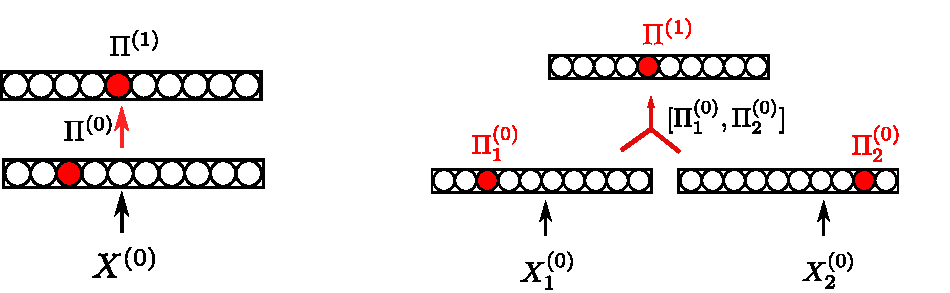
\includegraphics[width=\textwidth]{HSOM.pdf}
    \caption{Architecture HSOM \cite{lampinen_clustering_1992}. L'apprentissage des positions du BMU de la première couche par la seconde permet de mieux détecter les ensembles de données, dans une tâche de clustering. La deuxième couche est vue comme un niveau plus abstrait que la première. \label{fig:hsom}}
\end{figure}

\begin{figure}
    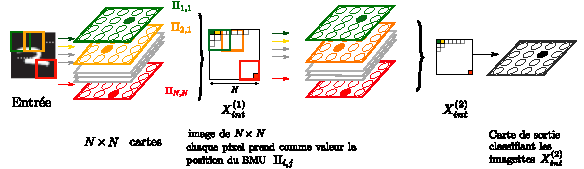
\includegraphics[width=\textwidth]{DSOM.pdf}
    \caption{Architecture DSOM de SOM "convolutionnelle" \cite{liu_deep_2015}. Les auteurs utilisent les positions des BMUs de la couche de carte $j_{p,q}$ comme valeurs d'entrée pour les couches suivantes, dans la lignée de HSOM \cite{lampinen_clustering_1992}. Les couches sont entraînées les unes après les autres. Cette architecture est \emph{feedforward} et \emph{hiérarchique} par transmission de représentation intermédiaire. \label{fig:dsom}}
\end{figure}

Toutes les architectures présentées ici, comme pour les architectures sélectives, sont feed-forward: les couches sont entraînées les unes après les autres. 
Par conséquent, elles ne se prêtent pas à un apprentissage en ligne, tout comme une carte de Kohonen classique.
La plupart des travaux sont appliqués à des tâches de classification qu'on pourrait réaliser avec une SOM classique.
La motivation d'utiliser une architecture plutôt qu'une SOM est alors que la couche finale du réseau possède de meilleures performances en termes de classification que si on avait utilisé une SOM simple.

% Aly ? evoque des perfs similaire à un réseau de deep learning supervisé
% Note : pour une tache de classification, une carte peut eytre comparée à un algo supervisé: la phase de choix de la classe est gérée par un algorithme supervisé après entrainement de la carte.

Nous pouvons conclure de ces travaux qu'il existe différentes façons de transmettre des informations entre couches. Les plus courantes sont la transmission de la position du BMU comme entrée pour la carte suivante, ou un calcul d'activation prenant en compte l'activation de la couche précédente par une connexion neurone à neurone.
La transmission de la position du BMU dans HSOM, Deep SOM et de nombreux autres travaux nous semble particulièrement intéressante car elle exploite totalement l'aspect topologique d'une carte de Kohonen. Par ailleurs, il s'agit d'une valeur de faible dimension, donc se prêtant à des calculs. Les architectures telles que Deep SOM nous montrent qu'une architecture utilisant seulement ce type d'information comme interface est capable de bonnes performances en reconnaissance d'image.
Le champ d'application des architectures feed-forward est le même qu'une SOMs classique~: quantification vectorielle et classification. Leurs performances dans ces domaines surpassent alors celles d'un SOM classique, la présence de couche multiples créant un nouveau niveau d'abstraction.

Nous pouvons donc considérer ces architectures comme des améliorations de carte auto-organisatrices sur des applications spécifiques. Elles n'ont pas la capacité de faire d'autres types de calcul que ceux originalement réalisés dans une SOM.
L'aspect uniquement feed-forward en est la cause: les cartes intermédiaires agissent comme des filtres intermédiaires de l'information donnée en entrée, mais la couche finale reste une carte auto-organisatrice classique.
Cela nous amène à étudier des architectures comportant des boucles de rétroaction~; nous qualifierons ces architectures de non-hiérarchiques. Ces architectures, nous le verrons, permettent de diversifier les comportements d'apprentissage qu'il est possible d'obtenir avec des SOMs en apportant un aspect dynamique au système par les rétroactions.

% C'est l'avenement du deep learning qui a poussé à créer des archi de SOMs. De la meme facon que les réseaux profonds ont étendu les capacités d'apprentissage du perceptron, les couhes de SOM montrent la meme ppté.
% Est-ce que la recherche actuelle sur l'apprentissage non supervisé poussera à remettre les SOM au gout du jour ? Est-ce qu'on ne fait pas de deep som, simplement parce que les outils n'ont pas été développés comme ceux du deep learning ? L'aspect non linéaire d'une SOM peut pourtant etre prometteuse dans ce cadre d'applis.
% Il s'agit par contre d'archiectures completement feed forward: on ne peut pas vraiment parler d'archi modulaires. Les couches sont apprises les unes après les autres.
% On fera référence à ce type d'archis comme des archis hiérarchiques.
% ces arhcitectures montrent des capacités d'apprentissage de motifs à plus grande echelle qu'une carte simple.

% \begin{itemize}
%     \item Historique de l'assemblage des SOMs en architectures feedforward ? 
%     \item Quels sont les avantages apportés par les deep SOMs par rapport à des Soms classiques
%     \item Quels sont les avantages des deep SOM par rapport aux réseaux de deep Learning 
%     \item Pourquoi ne sont elles pas plus utilisées maintenant ?
% \end{itemize}

\subsection{Structures de cartes auto-organisatrices non-hiérarchiques}

Les architectures non-hiérarchiques de SOMs sont des architectures comportant plusieurs cartes communiquant entre elles et dont le schéma de connexion comporte des boucles de rétroaction~: une carte A reçoit de l'information d'une carte B, qui elle-même reçoit de l'information de la carte A.
Ces architectures sont souvent proposées par une motivation d'inspiration biologique, dans le domaine des neurosciences computationnelles, en s'appuyant sur les théories mentionnées précédemment de la réentrée \cite{Edelman1982GroupSA} et des zones de convergence-divergence (CDZ) \cite{damasio_time-locked_1989}.
L'assemblage de réseaux de neurones en architecture fait l'objet de plus nombreux travaux dans le domaine des neurosciences computationnelles. Nous ne détaillerons pas ces travaux ici, nous intéressant spécifiquement aux modèles computationnels destinés à être appliqués en informatique et non modélisant finement la biologie.

Nous avons pu distinguer deux types d'architectures non-hiérarchiques dans l'état de l'art.
Certaines architectures comportent des cartes sensorielles qui sont reliées via des cartes associatives ne prenant pas d'entrées sensorielles, mais seulement des éléments de connexion interne. Ces architectures sont \emph{centralisées} dans la mesure ou ces cartes associatives centralisent l'information  montant des cartes sensorielles et la redistribuent. Ces architectures centralisées sont souvent désignées par leurs auteurs comme hiérarchiques~: en effet, les cartes associatives forment un niveau d'apprentissage différent des cartes sensorielles, apportant une hiérarchie dans l'apprentissage. Nous les classons ici dans la catégorie non-hiérarchique. Bien que des niveaux de cartes peuvent être isolés dans ces architectures, les connexions entre les cartes de deux niveaux sont bidirectionnelles, la carte associative étant à l'origine de l'activation de cartes sensorielles, et réciproquement.
Nous les différencions ainsi des cartes hiérarchiques feed-forward que nous avons listé au paragraphe précédent.
Le second type d'architectures non-hiérarchiques sont celles utilisant des connexions directes entre cartes sensorielles. Ces architectures sont \emph{décentralisées}~: il n'existe pas de module par lequel toute l'information transite.

Un point commun de toutes ces architectures non-hiérarchiques est leur champ d'application~: contrairement aux architectures hiérarchiques feed-forward qui cherchent à améliorer les performances de classification ou de \emph{clustering} d'une SOM classique, les SOM non-hiérarchiques que nous avons relevées dans la littérature sont plutôt appliquées à des tâches de \emph{mémoire associative} sur des données \emph{multimodales}. Ces cartes sont des systèmes dynamiques et ont la capacité de générer une valeur de sortie de façon autonome. Dans la mémoire associative, elles sont alors utilisées pour prédire une modalité à partir d'une autre.

\subsubsection{Architecture comportant une carte associative~: architecture centralisée}

L'idée d'assembler des cartes prenant en entrée une modalité sensorielle par une carte associative a été explorée en \cite{dominey13} et \cite{escobar-juarez_self-organized_2016}.
Dans ces deux travaux de neuroscience computationnelle, les auteurs construisent une architecture se voulant une modélisation du cadre CDZ, mais avec des cartes auto-organisatrices classiques, en transmettant les positions des BMU entre les cartes multimodales. 
Chacune des cartes possède plusieurs couches, chacune prenant une modalité en entrée. Une activité est calculée sur ces modalités en une activité commune. La position du BMU, en l'occurrence un vecteur 3D, sera utilisée comme modalité hiérarchique pour connecter des cartes entre elle. Les auteurs assemblent alors plusieurs cartes sensorielles grâce à des cartes associatives.
Dans le cas d'une hiérarchie de cartes, les auteurs entrainent les couches de l'architecture séparément~: les cartes modales du premier niveau sont apprises, puis la carte amodale les connectant est apprise dans un second temps. 
Une fois toute les cartes apprises, la structure est utilisée pour activer une ou des modalités en activant la carte amodale. Cette carte représente la zone de convergence divergence des modèles cérébraux. 
Dans ce modèle, les cartes sensorielles sont d'abord entraînée, puis les cartes associatives sont apprises dans un second temps. Nous l'avons quand même classée comme non-hiérarchique, car une fois que toutes les connexions sont apprises, elle permet des rétroactions entre cartes. 

Les travaux conduits précédemment dans notre équipe de recherche sur les architectures de cartes auto-organisatrices se classent dans cette catégorie. Ainsi, l'architecture Bijama développée en \cite{menard05,khouzam_2013},associe des cartes modales par une carte associative par des connexions neurone à neurones, en renforçant les connexions entre les groupes de neurones s'activant au même moment dans les cartes modales, via la carte associative.
Notons que Bijama repose sur des calculs complètement locaux, y compris au sein d'une carte auto-organisatrice.



\begin{figure}
    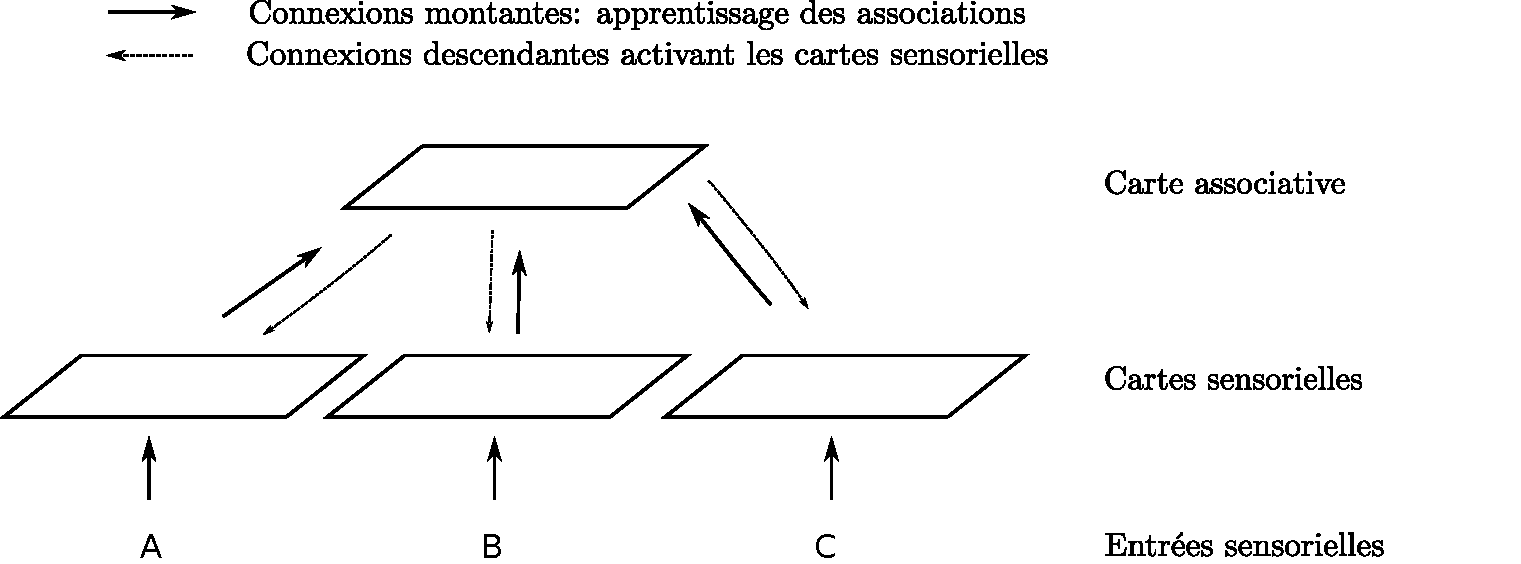
\includegraphics[width=\textwidth]{archi_associative.pdf}
    \caption{Exemple général d'architecture décentralisée comportant une carte associative. Ces architectures sont utilisées dans des tâches de traitement de données multimodales.
     Des cartes appelées cartes \emph{sensorielles} ou \emph{modales} prennent des entrées dans plusieurs modalités. Une carte \emph{associative} reçoit des connexions montantes de ces cartes et apprend à associer les activités. Les cartes sensorielles sont connectées à la carte associative par des connexions descendantes pouvant générer une activation dans la carte. Dans la plupart des modèles, les connexions montantes et descendantes n'ont pas le même rôle: les cartes sensorielles ne s'influencent pas entre elles lors de l'apprentissage.
     Lors de l'utilisation de l'architecture pour de la génération d'entrée sensorielle, alors les connexions descendantes permettent à la carte associative d'activer une carte sensorielle. \label{fig:archi_associative}
     }
\end{figure}

\begin{figure}
    \centering
    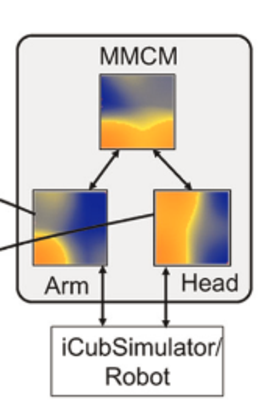
\includegraphics[width=0.3\textwidth]{MMCM_schema.pdf}
    \caption{Architecture MMCM. Les cartes du premier niveau reçoivent l'une les mouvements de tête d'un robot, l'autre les mouvements de main. 
    Une carte amodale (MMCM) reçoit les positions des BMUs de chaque carte du premier niveau. Chaque carte du premier niveau possède également une couche "hiérarchique" prenant en entrée les positions du BMU de MCMM. Chaque niveau est entrainé séparément.
    Après apprentissage, l'activation de la carte MCMM produit des mouvements coordonnés tête/mains~\cite{dominey13}\label{fig:mmcm}}
\end{figure}

Les modèles mentionnés ci-dessus rentrent dans la catégorie non-hiérarchique pour leur possibilité d'activation d'une carte par l'autre. Encore une fois, la position du BMU apparaît chez \cite{dominey13} comme le vecteur de transmission d'information  entre cartes et suffit pour que la coactivation des cartes permettent de réaliser de la mémoire associative. Le modèle SOIMA et le modèle Bijama privilégient la connexion neurone à neurone entre la carte associative et la carte modale, avec une règle d'apprentissage Hebbienne.
Cette mémoire associative est utilisée dans un cadre de données multimodales, avec une notion d'activation d'une carte par l'autre, contrairement aux architectures hiérarchiques citées en section précédentes, utilisées plutot pour des tâches de classification, autrement dit des tâches supervisées.
Dans ces exemples architectures présentées ici, on considère les cartes comme des représentations de leur espace de données qui permettent de la coactivation entres cartes~: une carte de Kohonen prend une fonction générative.

La présence de cartes associatives au sein d'une architecture crée une centralisation de l'information multimodale sur une carte, ce qui nous amène à parler d'apprentissage centralisé. Chaque carte sensorielle ne reçoit aucune information directe d'autres cartes de l'architectures, sauf de la carte associative.

Face aux architectures centralisées, nous pouvons imaginer des architectures décentralisées implémentant des connexions directes entre cartes modales.

\subsubsection{Architectures non-hiérarchiques décentralisées}

Nous avons relevé peu de travaux portant sur des architectures décentralisées, c'est-à-dire comportant des connexions directes entre cartes sensorielles. Un exemple générique d'architecture décentralisée est tracée en figure~\ref{fig:archi_decentralisee}. Les architectures proposées dans tous les travaux que nous avons relevés sont appliquées à de l'apprentissage multimodal.

Une première façon d'associer des cartes de Kohonen est de connecter les neurones d'une carte aux neurones d'une autre par des connexions pondérées. C'est par exemple ce qui est proposé dans \cite{khacef_brain-inspired_2020}. Les auteurs utilisent ici des cartes de Kohonen impulsionnelles, plus directement inspirées de la biologie que les cartes de Kohonen classiques, mais les mêmes principes d'auto-organisation se retrouvent entre les deux modèles. Dans ces travaux, les auteurs apprennent ainsi deux modalités d'un espace multimodale sur deux cartes auto-organisatrices, l'image et le son, puis dans un second temps apprennent les connexions entre neurones en mettant leurs poids à jour à partir des paires d'entrées image-son. Les neurones de chaque carte s'activant sur une même paire d'entrées voient le poids de leur connexion se renforcer, et inversement.
Les auteurs montrent que cette architecture permet d'apprendre les associations d'entrées et peut générer une entrée à partir de l'autre. 
Ce modèle est très simple mais sa mise à jour doit être réalisée en plusieurs étapes~: d'abord les poids des cartes, puis les poids des connexions. Cet apprentissage en deux temps était également présent dans l'architecture centralisée de \cite{dominey13}.

Nous remarquons par contre deux modèles qui cherchent à créer une architecture décentralisée de carte dont l'apprentissage est réalisé d'une seule traite. 

\begin{figure}
    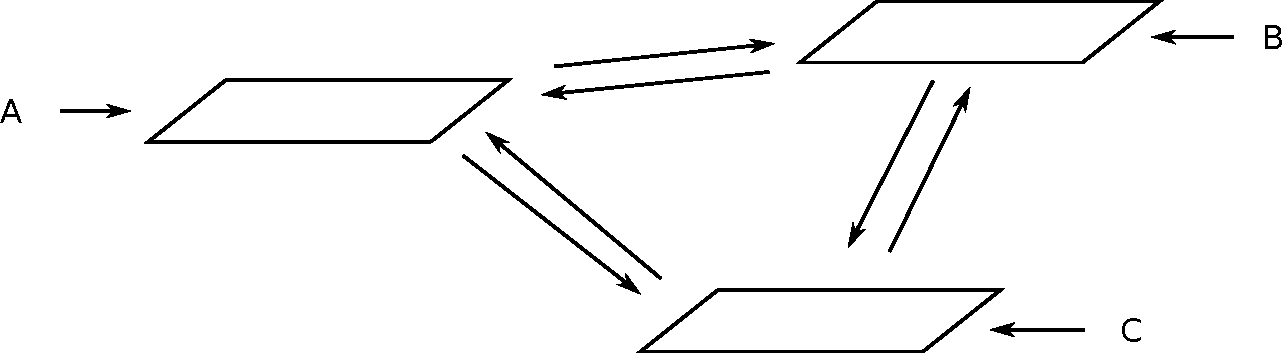
\includegraphics[width=0.9\textwidth]{archi_decentralisee.pdf}
    \caption{Exemple général d'architecture décentralisée de cartes. Chacune des cartes de l'architecture prend une entrée sensorielle A,B,C. Des connexions entre cartes permettent l'apprentissage d'associations entre modalités. Chacune des cartes peut donc être vue comme une carte multimodale. La façon de gérer les rétroactions entre cartes varie en fonction des travaux et est une problématique majeure dans la construction d'une telle architecture. Ainsi, les cartes apprennent à associer leurs activités seulement après avoir appris les modalités en \cite{khacef_brain-inspired_2020} et conjointement en \cite{johnsson_associative_2009} et \cite{baheux_towards_2014}.\label{fig:archi_decentralisee}}
\end{figure}

Une telle version d'architecture de cartes non-hiérarchiques est développée en \cite{johnsson_associating_2008,johnsson_associative_2009}, sous le nom de A-SOM, \emph{associative self-organizing map}. Encore une fois, le but d'une telle architecture est de faire de l'apprentissage multimodal, en apprenant à associer les activités de cartes sur différentes modalités. La particularité de A-SOM, par rapport à tous les modèles précédemment étudiés, est que l'apprentissage de toutes les cartes et de leurs interactions est réalisé simultanément. Ce modèle décentralisé inclut la possibilité de créer une version d'architecture centralisée à partir des règles d'associations, par exemple \cite{buonamente_hierarchies_2016}. Ainsi, un modèle d'architecture décentralisé est intéressant pour la recherche de nouveaux comportements dans la mesure où il n'impose pas de structure spécifique pour l'architecture. La structure des connexions entre cartes devient alors un paramètre sur lequel on peut complètement agir, contrairement aux architectures centralisées.
Une carte du modèle A-SOM possède plusieurs couches de poids. L'une de ces couches est relative à l'entrée de la SOM provenant du capteur. L'autre couche de poids reçoit une entrée provenant d'une autre carte de l'architecture. L'information transmise ici est l'activation de tous les neurones de l'autre carte. chaque carte reçoit ainsi $N\times M$ valeurs d'activité. L'interface entre cartes utilisée en A-SOM est donc le champ d'activation des neurones.

\begin{figure}
    \centering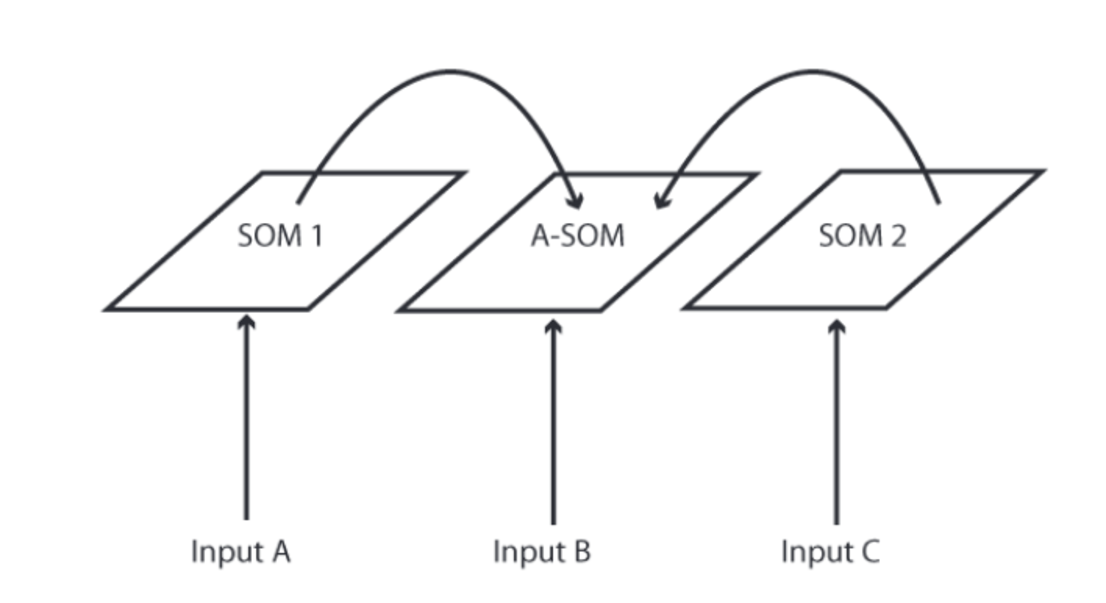
\includegraphics[width=0.7\textwidth]{A-SOM.pdf}
    \caption{Le modèle A-SOM \cite{johnsson_associative_2009} associe les activités de différentes cartes. Chacune des cartes prend une modalité A,B,C en entrée. Contrairement aux modèles précédemment cites, les trois cartes apprennent simultanément. L'association est prise en compte lors du calcul des activités de chaque carte.\label{fig:asom}}
\end{figure}

L'architecture développée en \cite{lefort_active_2015} implémente également une architecture décentralisée pour de l'apprentissage multimodal. De façon similaire à A-SOM, les auteurs associent plusieurs poids aux neurones d'une carte, chacun des poids étant relatif à un type d'entrée~: l'entrée modale et l'entrée venant d'autres cartes. L'information transmise dans ce cas est une partie de l'activité des neurones, celle située dans un carré centré à la même position que le neurone courant. L'information transmise entre cartes est ainsi également un champ d'activation.

\subsubsection{Des modèles multicartes incluant des connexions temporelles}

Certains modèles s'appuient sur plusieurs cartes de Kohonen connectées, en y ajoutant une notion de traitement de séquences.
en \cite{parisiLL}, les auteurs développent une architecture de deux réseaux auto-organisés appelés \emph{grow when required networks} (GWR). Ces réseaux sont des versions incrémentales de cartes de Kohonen dans lesquelles des neurones sont ajoutés au cours de l'apprentissage, le processus de recherche de BMU restant ensuite similaire à une SOM classique.
Cette architecture utilise deux réseaux GWR pour apprendre des séquences, formant une mémoire épisodique et une mémoire sémantique.
La carte associée à la mémoire épisodique (G-EM) est une version récurrente du GWR, dans laquelle des connexions temporelles entre neurones sont mises à jour en supplément des poids associés aux neurones. Le BMU est alors choisi en fonction de l'entrée courante ainsi que des BMUs précédent. 
La deuxième carte est une version classique du GWR. Elle prend en entrée une séquence de BMUs de la carte G-EM, ainsi que la classe de la séquence courante, afin de mettre à jour ses poids. 
Cette architecture associe ainsi des connexions temporelles récurrentes sur une carte ainsi que des connexions entre cartes.
Cette architecture permet des tâches de \emph{lifelong learning}. 
Le concept d'apprentissage sur le long terme s'intéresse à des systèmes étant mis à jour en ligne, dès qu'ils recoivent une entrée, et dont l'apprentissage n'a pas de limite temporelle fixé. On doit donc avoir un système qui trouve de lui-même une stabilité dans l'apprentissage et qui est capable de s'adapter à de nouvelles entrées.
Dans la plupart des applications en robotique, les entrées présentées à une structure d'apprentissage sont par ailleurs des entrées ayant une relation temporelle. Deux images recues successivement par un capteur visuel seront proches dans l'espace des images. Pour une SOM par exemple, cela pose problème. Les archcitectures de lifelong learning cherchent donc une solution à ces problèmes pour créer une structure autonome, évoluant dans le temps et permettant de réaliser la tâche pour laquelle elle est conçue tout en continuant à être mise à jour, sans oublier les données vues au début de l'apprentissage.
Les auteurs utilisent leur architecture pour de la reconnaissance d'objets. Cependant, lors de l'apprentissage, les données ne sont pas présentées après un tirage aléatoire dans l'espace, mais sont présentés classe par classe~: tous les objets d'une même classe d'abord, etc. Les auteurs montrent que l'architecture est capable de bien prédire la classe d'un objet lors d'un test sur toutes les classes apprises. \`{A} titre de comparaison, une SOM classique apprendrait la classe du premier objet, puis l'oublierait pour se déplier entièrement sur la deuxième classe, etc. A terme, seule la dernière classe apprise est gardée en mémoire.

La motivation de ces modèles multicartes est intéressante~: il s'agit cette fois de voir les deux cartes comme de l'apprentissage à différentes échelles temporelles. L'architecture mélange connexions récurrentes et connexions inter-cartes, ce qui est pertinent dans le cadre de l'apprentissage de séquence, et dans le but de création de systèmes autonomes de cartes auto-organisatrices évoquées par Kohonen. 
Cependant, si sa motivation nous intéresse, le modèle décrit précédemment utilise une logique de vérification externe aux cartes pour ajouter ou nom des neurones. 

Notre démarche s'inscrit dans un objectif d'allier connexions temporelles et connexions intercartes au sein d'une même architecture, sans forcément avoir à différencier ces connexions.
Les travaux autour du modèle A-SOM mentionné précédemment en ont ainsi dérivé une version récurrente \cite{Buonamente2015DiscriminatingAS}. Cette version récurrente est similaire à la version multicarte. Au lieu de considérer l'activité d'une autre carte pour le calcul de l'activité courante d'une carte, les auteurs utilisent l'activité de la même carte à l'état précédent.
Cette structure est appliquée à la prédiction de mouvement. De la même façon qu'une architecture est capable, à partir d'une modalité, de prédire les valeurs correspondant à l'autre modalité, l'architecture incluant une version récurrente peut prédire la fin d'une séquence à partir de son début. La motivation de développer une version récurrente de A-SOM est alors de pouvoir développer des architectures comportant connexions récurrente et connexions intercartes. Nous n'avons pas encore relevé cependant de travaux les intégrant effectivement dans une architecture multicartes.

Les travaux menés en \cite{baheux_towards_2014} ont également cherché à insérer des connexions temporelles au sein d'une architecture de deux cartes, présentée en \ref{fig:baheux}. Chaque carte est composée de deux couches de poids. Une des cartes prend une entrée correspondant à l'observation courante, relative à une première couche de poids, comme une SOM classique. La deuxième couche de poids est relative à l'information interne descendant de la seconde carte, qui est la position du BMU de la deuxième carte. 
La seconde carte recoit deux entrées de la première~: une entrée est la position du BMU de l'état précédent et la seconde la position du BMU de l'état courant. Une activité est calculée sur chaque couche de poids relativement à son entrée et ces deux activités sont fusionnées en une activité globale à chaque carte.
Comme chaque carte reçoit en entrée la position de l'état courant du BMU de l'autre carte, il existe une boucle de rétroaction entre carte. Les auteurs laissent alors "résonner" les activités en déplacement petit à petit les BMUs de chaque carte, jusqu'à obtenir un état stable pour les activités, qui est utilisé pour déterminer le BMU final servant à la mise à jour des poids. 
Ce modèle permet alors d'apprendre des séquences d'entrée. Alors qu'une carte simple différencierait les BMUs en fonction de la valeur de l'entrée, ce modèle génère une différenciation des BMUs en fonction de la position d'un élément dans la séquence en plus de sa valeur. 


\begin{figure}
    \centering
    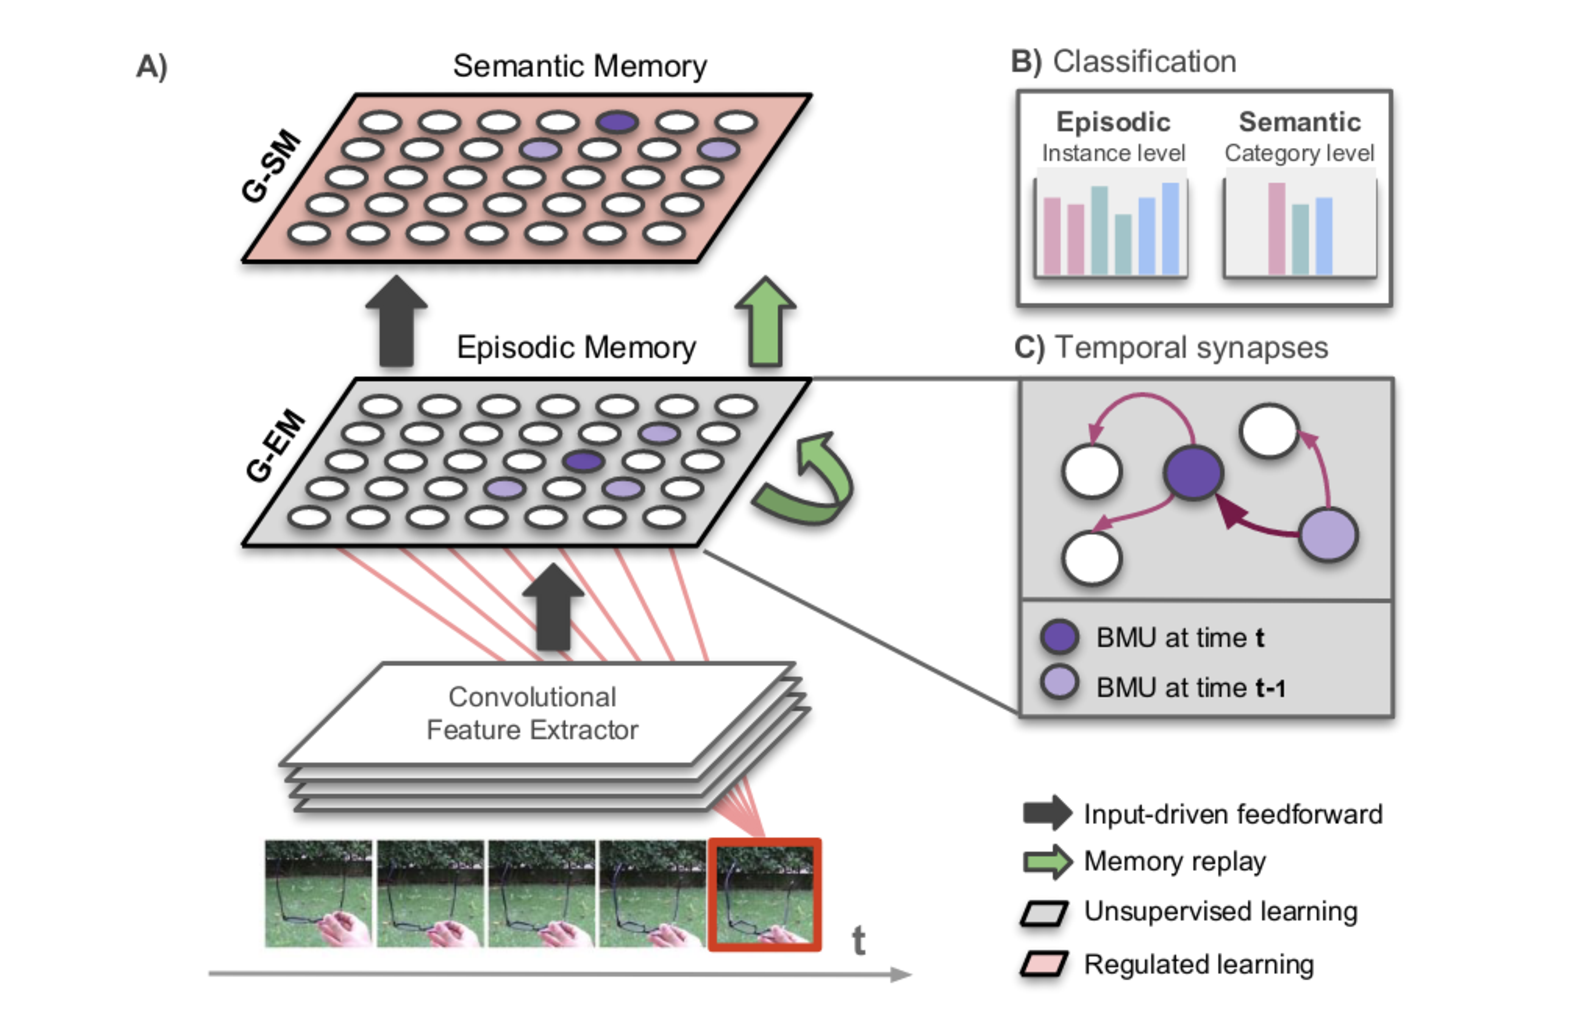
\includegraphics[width=0.8\textwidth]{Parisi_2020.pdf}
    \caption{Architecture \emph{à double mémoire} proposée en \cite{parisiLL}. La couche de mémoire épisodique est un réseau \emph{grow when required (GWR)}, un réseau auto-organisé similaire à une carte de Kohonen, à la différence que les neurones sont ajoutés au fur et à mesure de l'apprentissage. La couche de mémoire sémantique est également un réseau GWR, entraîné à partir des BMUs de la couche épisodique et de la classe de la séquence jouée. L'architecture apprend à reconnaitre plusieurs séquences.\label{fig:gdm_parisi}}
\end{figure}

\begin{figure}
    \centering
    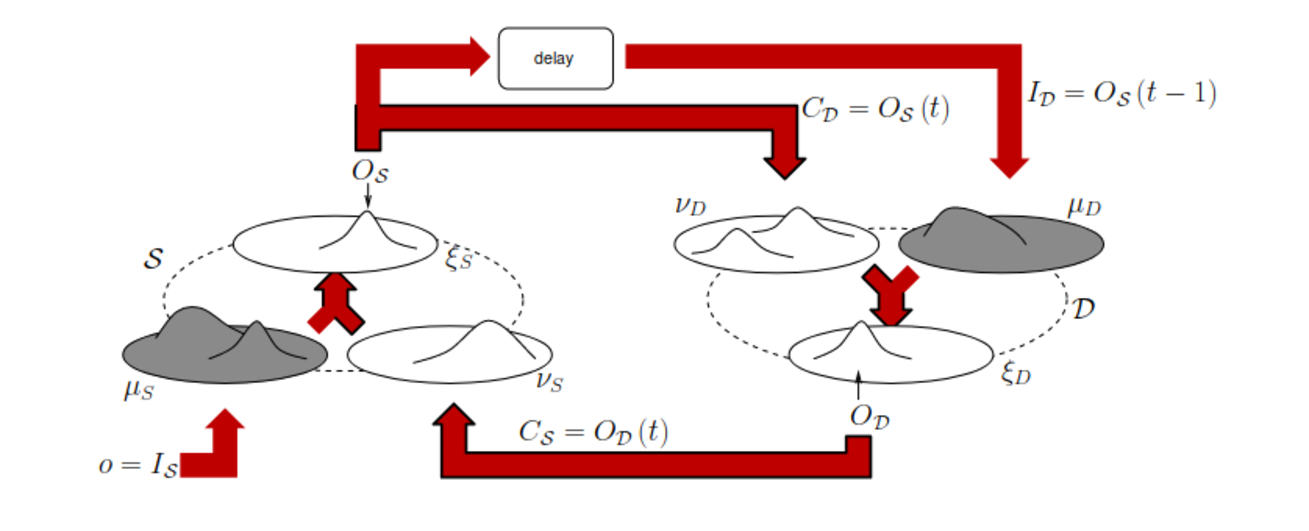
\includegraphics[width=0.8\textwidth]{baheux.pdf}
    \caption{Structures de deux cartes auto-organisatrices communicantes, \cite{baheux_towards_2014}. Chaque carte est composée de trois couches d'activités, représentées séparément sur le schéma: sur la première carte, une activité est relative à l'entrée $o$, l'observation. L'autre activité reçoit une entrée descendant de la seconde carte. Ces deux activités sont fusionnées en une activité globale servant à déterminer un BMU. La seconde carte reçoit ensuite deux entrées venant de la première carte : le BMU de l'état courant et le BMU de l'état précédent. Un système de résonnance est mis en place pour gérer les boucles de rétroactions entre BMUs, comme chaque carte reçoit le BMU de l'état courant de l'autre carte en entrée. Ce principe laisse évoluer dynamiquement les activités vers un état stable, utilisé ensuite pour la détermination du BMU final.\label{fig:baheux}}
\end{figure}

Ces exemples nous amènent à pousser la bibliographie de cette thèse sur les cartes de Kohonen récurrentes. On voit en effet la similarité existant dans le traitement de séquences, ou le choix d'un BMU doit prendre en compte le contexte des états précédents, aux modèles multimodals dans lequel le choix d'un BMU doit prendre en compte le contexte des entrées d'autres modalités. 

\subsection{Cartes auto-organisatrices récurrentes}

\begin{figure}
   \centering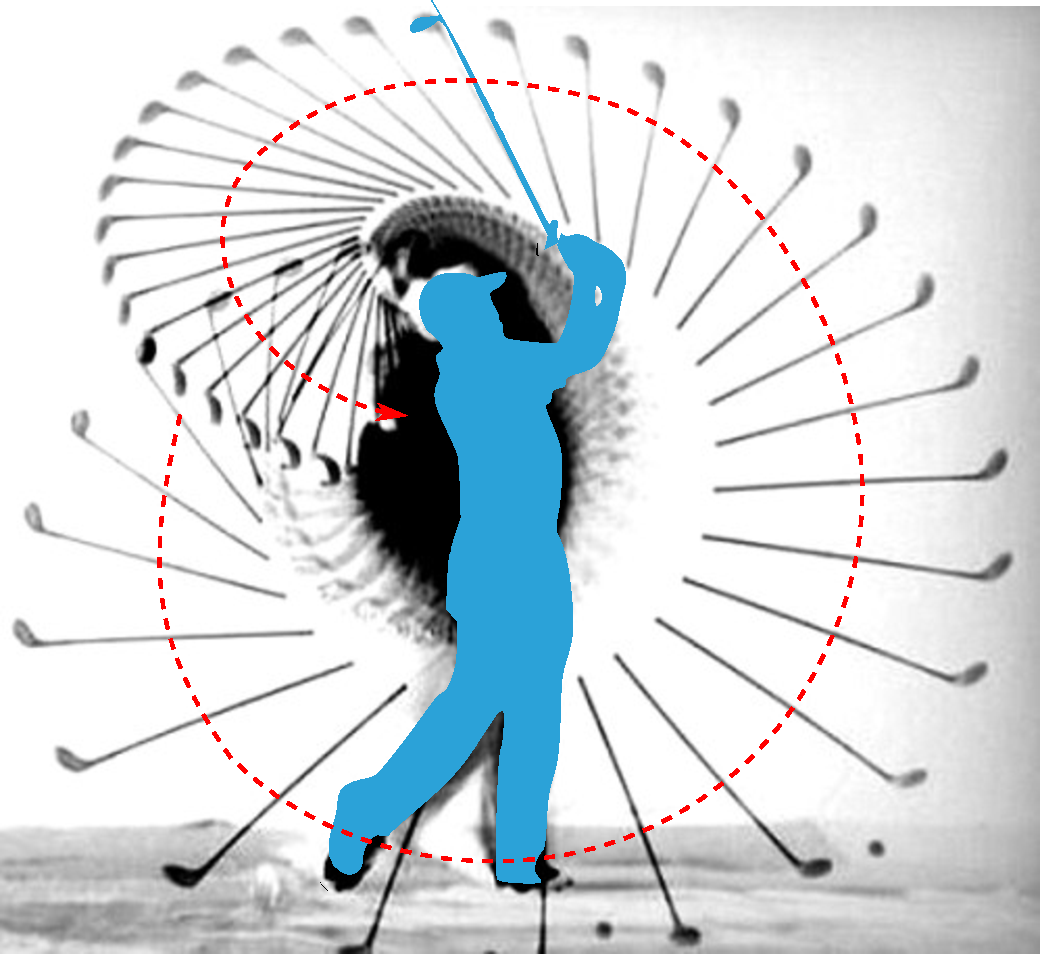
\includegraphics[width=0.6\textwidth]{movment_002.pdf}
   \caption{L'image présentée à un réseau (en bleu) correspond à un instant d'une séquence. L'objectif de l'apprentissage non-supervisé de séquences est d'extraire une représentation d'une séquence d'entrée. Une utilisation commune est la classification de mouvements. La séquence "tirer" sera différente de la séquence "marcher".\label{fig:mouvement}}
\end{figure}

On appelle réseaux récurrents des réseaux de neurones qui prennent en compte leur état précédent pour calculer leur état actuel. Ces réseaux sont utilisés pour le traitement et l'apprentissage de signaux temporels. Citons par exemple, en Deep Learning, les RNN (\emph{recurrent neural networks}), dont les neurones reçoivent leur état précédent en entrée. Les cartes de Kohonen ont ainsi également des versions récurrentes.

Nous nous intéressons aux architectures multicartes, mais les cartes récurrentes répondent à des problèmes très similaire à ceux rencontrés dans la conception d'architectures de cartes pour faire de la mémoire associative, comme vu en section précédente.
Dans une carte récurrente, le problème principal est de trouver comment communiquer à la carte de l'information sur son état précédent et comment utiliser cette information dans l'apprentissage de l'état courant. Cela rejoint la problématique posée dans les architectures de cartes de Kohonen, qui est de comment communiquer à une autre carte son état, afin de l'utiliser dans l'apprentissage de l'état courant. L'étude des modèles de cartes récurrentes existant nous permettrons de compléter cette bibliographie. 

Notre volonté de créer un modèle général d'architecture de cartes auto-organisatrice motive également le fait de s'intéresser aux cartes récurrentes. On souhaite en effet créer un modèle qui puisse unir cartes récurrentes et cartes normales au sein d'une même architecture. L'aspect bio-inspiré du modèle et son aspect multimodal ciblent plutot des applications d'un tel réseau en robotique. Or, la plupart des données traitées par des réseaux de neurones, en particulier dans les applications robotiques, sont temporelles : vidéos, signaux sonores, capteurs de position. Il est donc important de s'appuyer autant sur les modèles de cartes récurrentes existantes que sur les architectures afin de créer un modèle général.

Les modèles de cartes récurrentes existant dans la littérature se classent en catégories similaires aux modèles multicartes que nous avons listé.
D'une part, certains modèles de cartes utilisent l'état précédent de la carte lors du calcul de \emph{l'activité} de l'état courant. De l'autre, des modèles réutilisent plutôt des éléments de la carte à l'instant précédent directement en tant qu'\emph{entrée} de l'état courant.


Parmi les premiers travaux autour des cartes auto-organisatrices, l'Hypermap \cite{Kohonen1991THEHA}, dérivée ensuite en \emph{recurrent SOM} \cite{varsta_temporal_2001} conditionnent la recherche de BMU d'une carte à un contexte dépendant de l'état précédent, lié à l'entrée précédente dans la séquence. Ce contexte repose sur la limitation d'une zone de la carte dans laquelle faire la recherche du BMU. 

D'autres travaux reposent sur la transmission d'un contexte en tant qu'entrée complétant l'entrée courante. 
Ainsi, les \emph{recursive SOMs} de \cite{Voegtlin2002RecursiveSM} prennent deux entrées~: l'élément de la séquence ainsi qu'un vecteur contenant l'ensemble des activations des neurones de la carte à l'état précédent.
MSOM, de \cite{Strickert2005MergeSF} s'appuie sur le poids du BMU. A chaque instant, l'entrée de contexte à transmettre à l'état suivant est définie comme une combinaison linéaire entre le poids du BMU courant et le contexte courant.
Le modèle SOMSD \cite{hagenbuchner_self-organizing_2003, hammer_recursive_2004,hammer_self-organizing_2005, fix20} réduit ce contexte à la position de la Best Matching Unit.
Les travaux de \cite{Buonamente2013SimulatingAW} proposent une version récurrente du modèle A-SOM présenté en section précédente. Le contexte considéré est alors un ensemble d'activités de neurones.
Les mécanismes de transmission de contexte entre instants dans les cartes récurrentes s'appuient sur les mêmes mécanismes que ceux proposé dans le cadre d'architectures de cartes~: sélection de région de la carte, transmission d'activation, et enfin transmission du BMU.
Les travaux menés en \cite{fix20} sur le modèle SOMSD montrent qu'une carte récurrente parvient à différencier ses BMUs en fonction de la position de l'entrée dans une séquence et non seulement de la valeur de l'entrée.

\section{Axe de recherche}

Nous avons détaillé la littérature existante en terme d'architecture de SOMs et plus généralement de réseaux de neurones auto-organisés. Nous avons divisé ces architectures en deux grandes catégories~: un format hiérarchique et \emph{feedforward}, et un format non-hiérarchique incluant des rétroactions.
Le format feed forward implique généralement un apprentissage couche par couche. Ce format est très appliqué et permet d'améliorer les capacités de clustering d'une SOM classique, principalement dans le cas ou les données traitées présentent elles-mêmes une structure hiérarchique, telles que des images ou des phrases.
Nous cherchons à développer une architecture plus générale de cartes auto-organisatrices et ne nous placons ainsi pas dans le contexte des Deep SOM mentionné ci-dessus. 
Cependant, nous notons que la position du BMU comme interface entre couche de cartes permet des capacités de calcul.
Nombre de ces architectures sont développées directement dans un but applicatif. On peut ainsi faire la distinction entre un modèle d'architecture, tel que HSOM, qui est générique et applicable à tout type de données, et une structure appliquée, développées spécifiquement pour un type de données.

Opposées à ces architectures hiérarchiques, des architectures reposent sur de l'interaction entre cartes, avec des boucles de rétroaction.
Ces architectures sont moins présentes dans la littérature que les Deep SOM, et cherchent en général à se rapprocher d'un contexte biologique.
Nous nous plaçons plutôt dans la lignée des cartes non-hiérarchiques, sans vouloir cependant copier un aspect biologique.
De façon intéressante, nous remarquons que plusieurs structures non-hiérarchiques sont associées à l'apprentissage de données temporelles. Ces architectures se rapprochent des modèles appelés cartes auto-organisatrices récurrentes, dans lesquels des éléments de calcul d'une carte à une itération données sont réutilisés pour le calcul des itérations suivantes.
Ces architectures non-hiérarchiques dynamiques se divisent en architectures centralisées et décentralisées. La décentralisation des calculs va dans un sens de l'informatique non conventionnelle.

Ces modèles soulèvent également une problématique dans les algorithmes d'apprentissage d'architecture non-hiérarchiques comportant des rétroactions. Dans le cas des neurones impulsionnels, les impulsions des neurones arrivent en différé, une connexion réciproque entre neurones ne pose pas de problème~: les neurones sont traités dans l'ordre des impulsions. Dans le cas de cartes de Kohonen, qui ne repose pas sur des séries d'impulsions, l'information arrive simultanément dans les différentes cartes. L'activité de la carte A influence l'activité de la carte B, mais l'activité de la carte B influence également celle de la carte A, formant une boucle de rétroaction potentiellement infinie. Les architectures mentionnées font le choix d'apprendre d'abord les cartes sensorielles de façon indépendante, puis d'apprendre seulement leurs connexions dans un second temps, décomposant ainsi la boucle. 
La rétroaction est ensuite utilisée en phase applicative pour générer une modalité~: seule une des cartes sensorielle prend une entrée, l'autre carte est considérée comme la sortie de l'architecture et réagit à l'activité des autres cartes. Les rétro-actions ne sont alors pas non plus un problème en phase d'application.

Notons enfin que limites entre les catégories d'architectures que nous avons différenciées dans ce chapitre sont floues. Une architecture décentralisée peut contenir des sous-structures hiérarchiques ou au contraire, une structure hiérarchique de modules décentralisés peut être imaginée.

Parmi ces axes de développement d'architectures, nous choisissons de nous intéresser dans cette thèse à des architectures non-hiérarchiques de cartes.
Les architectures hiérarchiques nous paraissent de bonnes candidates à améliorer les performances d'une SOM sur une application spécifique comme du traitement d'images, tandis que les architectures non-hiérarchiques offrent de nouvelles possibilités de calcul, non envisageables par des SOM classiques, telles que la génération d'entrée, et c'est cet axe que nous souhaitons explorer.
%L'observation d'émergence de calcul dans des systèmes complexes d'apprentissage, introduite au chapitre~\ref{chap:modularite} vient appuyer ce concept.
Peu de travaux ont par ailleurs exploré l'idée d'associer des SOMs en architectures comportant des rétroactions.
Les choix pour la construction d'une telle architecture se situent au niveau de l'interface entre cartes. De nombreux travaux autour des cartes de Kohonen utilisent la position du BMU comme vecteur de l'information transmise entre plusieurs cartes. 
Nous faisons ce choix également. Il apparaît comme une valeur peu coûteuse à communiquer entre cartes, mais qui contient beaucoup d'information sur l'état d'une carte. Cette valeur se présente également comme un cadre homogène de communication intercarte: quelles que soient les entrées sur lesquelles apprend une carte, il sera toujours possible de la connecter à d'autres cartes de l'architecture. 
Enfin, on retrouve l'utilisation de la position du BMU à la fois dans des architectures multicartes et dans les cartes récurrentes comme SOMSD. Le cadre choisi permettrait donc d'intégrer à la fois des cartes classiques et des cartes récurrentes au sein d'une même architecture, offrant encore plus de possibilités de calcul.
Ce modèle de connexions par transmission de position de BMU n'a pas été exploré pour créer des architectures non-hiérarchiques décentralisées. Cette thèse se veut l'exploration de ce modèle.
Nos travaux font ainsi suite à \cite{baheux_towards_2014} sur des architectures récurrentes multimodales utilisant la transmission de la postion du BMU entre des cartes de Kohonen, exploitant la position du BMU comme les travaux sur les cartes récurrentes SOMSD \cite{hagenbuchner_self-organizing_2003,Strickert2003UnsupervisedRS,fix20}.
Les travaux commencés en \cite{baheux_towards_2014}, bien qu'ils exploitent des connexions intercartes, sont similaires à ce qu'on obtiendrait avec une carte récurrente simple, telle que celle décrite en \cite{fix20}.
Nous voulons continuer sur le même modèle, utilisant la transmission du BMU, qui nous apparaît comme une solution compacte et facilement extensible à grande échelle pour construire des grandes architectures, mais en explorant cette fois l'aspect des connexions intercartes.
Par leur motivation, qui est le développement d'un système multi-som, nos travaux se rapprochent aussi des travaux conduits sur l'architecture A-SOM \cite{johnsson_associating_2008, johnsson_associative_2009,gil_sarasom_2015, Buonamente2015DiscriminatingAS}~; notre modèle de carte et d'interface est par contre différent.



\begin{figure*}[b]
    \centering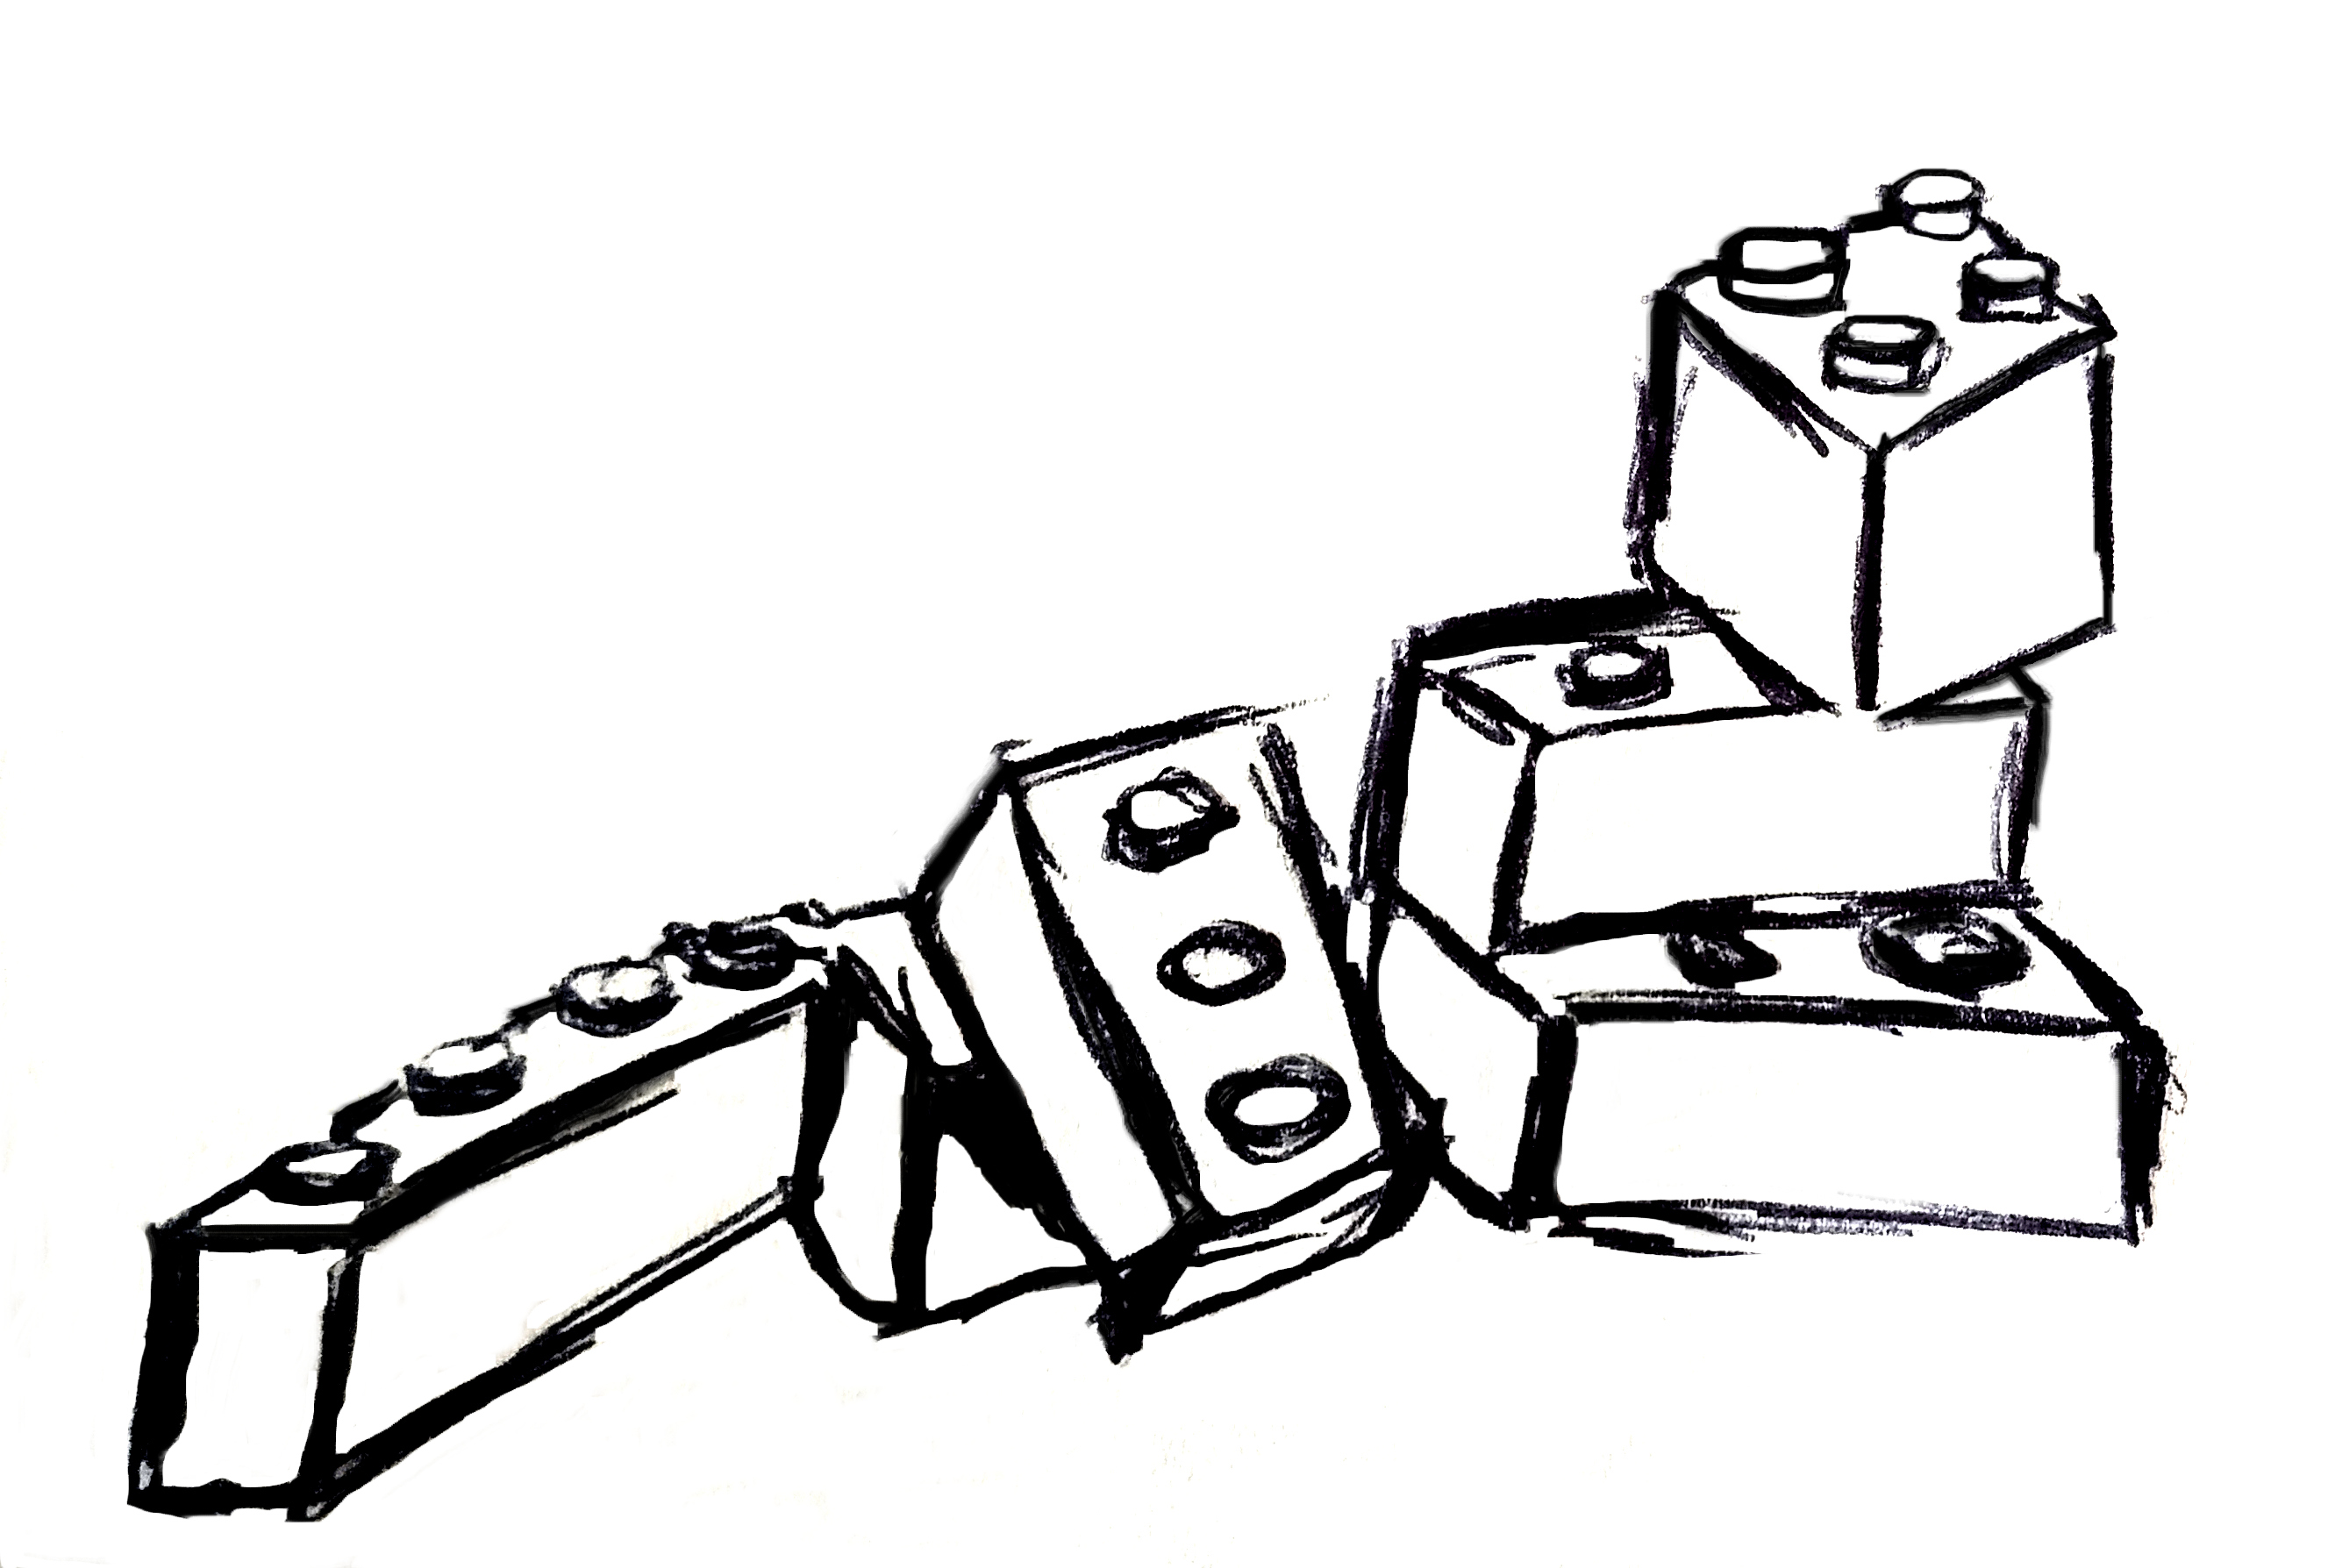
\includegraphics[width=0.6\textwidth]{lego2.jpg}
\end{figure*}

\ifSubfilesClassLoaded{
    \printbibliography
    %\externaldocument{../main.tex}   
}{}
\end{document}
%Chapitre en plus : multimodalité ?

\documentclass[../main]{subfiles}
\ifSubfilesClassLoaded{
    \dominitoc
    \tableofcontentsfile
    \setcounter{page}{1} 
    \setcounter{chapter}{1}
}{}
\begin{document}
\chapter{Modèle d'architecture CxSOM}{\label{chap:modele}}
\graphicspath{{03-SOM/},{./}}
\minitoc

\section{Introduction}

% Nous proposons dans cette thèse un modèle d'architecture non-hiérarchique de cartes auto-organisatrices, CxSOM. 
% \`A partir de ces architectures, nous cherchons à apprendre des relations entre des données issues de plusieurs modalités. 
% On souhaite que ce modèle soit générique, permettant de construire n'importe quel forme et taille d'architecture, et ayant la possibilité d'intégrer des connexions récurrentes. 
% Notre démarche est d'abord de proposer un modèle de calcul général à base de cartes auto-organisatrices~; des applications plus spécifiques pourront être développées à partir de cette méthode.

% Nous avons défini une architecture de cartes comme un réseau composé de plusieurs modules qui sont chacun une carte de Kohonen, et dans lequel des connexions sont présentes entre ces modules. 
% Ces connexions sont orientées: on parle d'une connexion d'une carte A vers une carte B. Le but de ces connexions est de coupler l'apprentissage de plusieurs cartes.
% Sur une telle architecture, on peut construire un graphe $G$ orienté, dont les n\oe{}uds sont des cartes. La connexion d'une carte A vers une carte B est indiquée par la présence d'une arête de A vers B. 
% On appelle architecture \emph{non-hiérarchique} une architecture pour laquelle le graphe $G$ n'est pas un arbre: il présente des boucles. Un exemple d'architecture non-hiérarchique est représenté en figure~\ref{fig:archi_non_hierarchique}. Certaines cartes sont connectées dans les deux directions, d'autres en boucle. 

% Dans cette thèse, nous cherchons à utiliser de telles architectures non-hiérarchiques pour des tâches de mémoire associative.
% Chaque carte de l'architecture cherche d'une part à apprendre une représentation de l'entrée $A,B,C,D,E$ ou $F$ qui lui est fournie. 
% Lorsque ces entrées présentent des dépendances les unes aux autres, l'architecture dans sa globalité doit également extraire les relations, les dépendances, existant entre les distributions de données. Cet apprentissage des relations est au c\oe{}ur de cette thèse, sa partie expérimentale se concentrant sur les représentations et indicateurs mettant en valeur l'apprentissage de ces relations puis en les utilisant sur différents ensembles de données d'entrée.
Dans ce chapitre, nous détaillons le modèle CxSOM que nous avons développé et étudié durant cette thèse. 
Nous définissons une version modifiée d'une carte auto-organisatrice, prenant des entrées externes et dont les règles d'évolution dépendent des autres cartes, ainsi que l'interface permettant d'assembler ces cartes au sein d'une architecture non-hiérarchique.

Des exemples de telles architectures sont présentés en figure~\ref{fig:archi_non_hierarchique}.
Nous détaillons en premier lieu le formalisme et les notations d'une carte de Kohonen classique, dont sont dérivées les cartes auto-organisatrices définies par CxSOM. 
Nous expliquons ensuite les choix de développement sur lesquels nous nous sommes appuyée pour développer le modèle. Nous présentons le modèle sur un exemple d'architecture à deux cartes, puis nous le formalisons pour le cas général de $n$ cartes connectées au sein d'une architecture.

\begin{figure}
\centering
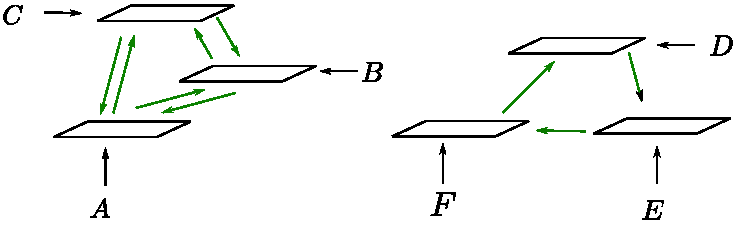
\includegraphics[width=0.6\textwidth]{architecture.pdf}
\caption{Deux exemples d'architectures \emph{non-hiérarchiques} à 3 cartes de Kohonen faisant figurer des connexions réciproques ou des boucles.
Les entrées fournies aux cartes sont $A,B,C,D,E,F$ quelconques.}
\label{fig:archi_non_hierarchique}
\end{figure}


\section{Carte de Kohonen classique}\label{sec:kohonen}

Chaque carte de Kohonen d'une architecture CxSOM est directement dérivée de l'algorithme d'une carte de Kohonen classique introduite en \cite{Kohonen1982}. Cet algorithme et ses dérivés sont décrits en détail par T. Kohonen dans son ouvrage~\parencite{Kohonen1995SelfOrganizingM}. Le principe général d'une carte de Kohonen a été décrit dans le chapitre précédent~; nous définissons ici plus précisément le modèle et les équations qui serviront de base pour la définition de l'algorithme CxSOM.

\subsection{Algorithme et notations}

Une carte de Kohonen est une grille de $N$ n\oe{}uds qui forme un \emph{mapping} d'un espace de faible dimension. 
Nous utiliserons dans cette thèse des cartes en une et deux dimensions, c'est-à-dire des lignes, cartographiant un espace 1D, et des grilles 2D. Les notations et le modèle présentés ici sont toutefois applicables à des cartes de dimensions quelconques.

L'algorithme et les notations sont résumés en figure~\ref{fig:one_map_not}. Une entrée fournie à une carte de Kohonen est notée $\inpx_t$, tirée dans un espace d'entrée $\mathcal{D}$. \`A chaque n\oe{}ud de la carte est associé un poids $\w_e \in D$, appelé aussi prototype. Sa \emph{position} dans la carte est indexée par $p$. Nous choisissons d'indexer les positions dans $[0,1]$~: l'ensemble des positions $p$ est donc un ensemble de points discrets entre $0$ et $1$. L'ensemble des poids est noté $\w_e(p)$. On peut faire la même discrétisation de l'espace $[0,1]^2$ pour une carte en 2D.

Chaque itération $t$ de l'algorithme de mise à jour d'une carte de Kohonen contient les étapes suivantes:
\begin{enumerate}
\item\label{enum:inp} Une entrée $\inpx_t$ est tirée et présentée à la carte.
\item\label{enum:act} Une \emph{activité} $a_e(p,\inpx_t)$ est calculée dans la carte pour chaque n\oe{}ud de position $p$. La fonction d'activité que nous utiliserons dans cette thèse est une activation gaussienne, définie par~:
\begin{equation}\label{eq:act1som}
a_e(p, \inpx_t) = \exp{\frac{-\lVert \inpx_t-\w_{e_t}(p) \rVert ^2}{2\sigma^2}}
\end{equation}
\item\label{enum:bmu} L'unité ayant l'activité maximale est la \emph{Best Matching Unit} de la carte. Sa position est notée $\bmu_t$.
\item Chaque poids $\w_e$ est déplacé vers l'entrée $\inpx_t$. Le déplacement est pondéré par une \emph{fonction de voisinage} $H_e(\bmu_t,p)$. Cette fonction est maximale en $p = \bmu_t$ et décroissante autour de cette position. Dans notre étude, la fonction de voisinage est triangulaire, maximale en $\bmu_t$, linéairement décroissante sur un \emph{rayon de voisinage} noté $h_e$ et nulle sinon.
\begin{equation}
\w_{e_{t+1}}(p) = \w_{e_t}(p) + \alpha H_e(\bmu_t,p)(\inpx_t - \w_{e_t}(p))
\label{eq:update}
\end{equation}
\end{enumerate}
% L'étape de calcul d'activité est déjà une modification de l'algorithme original de Kohonen.
% Dans la version classique, on calcule plutôt les distances entre l'entrée et les poids $\lVert \inpx_t - \w_e(p) \rVert$, et le BMU est choisi comme l'unité dont le poids présente la plus petite distance à l'entrée. 
% Ici, on prendra comme BMU l'unité ayant l'activité la plus élevée.

\begin{figure}
\centering
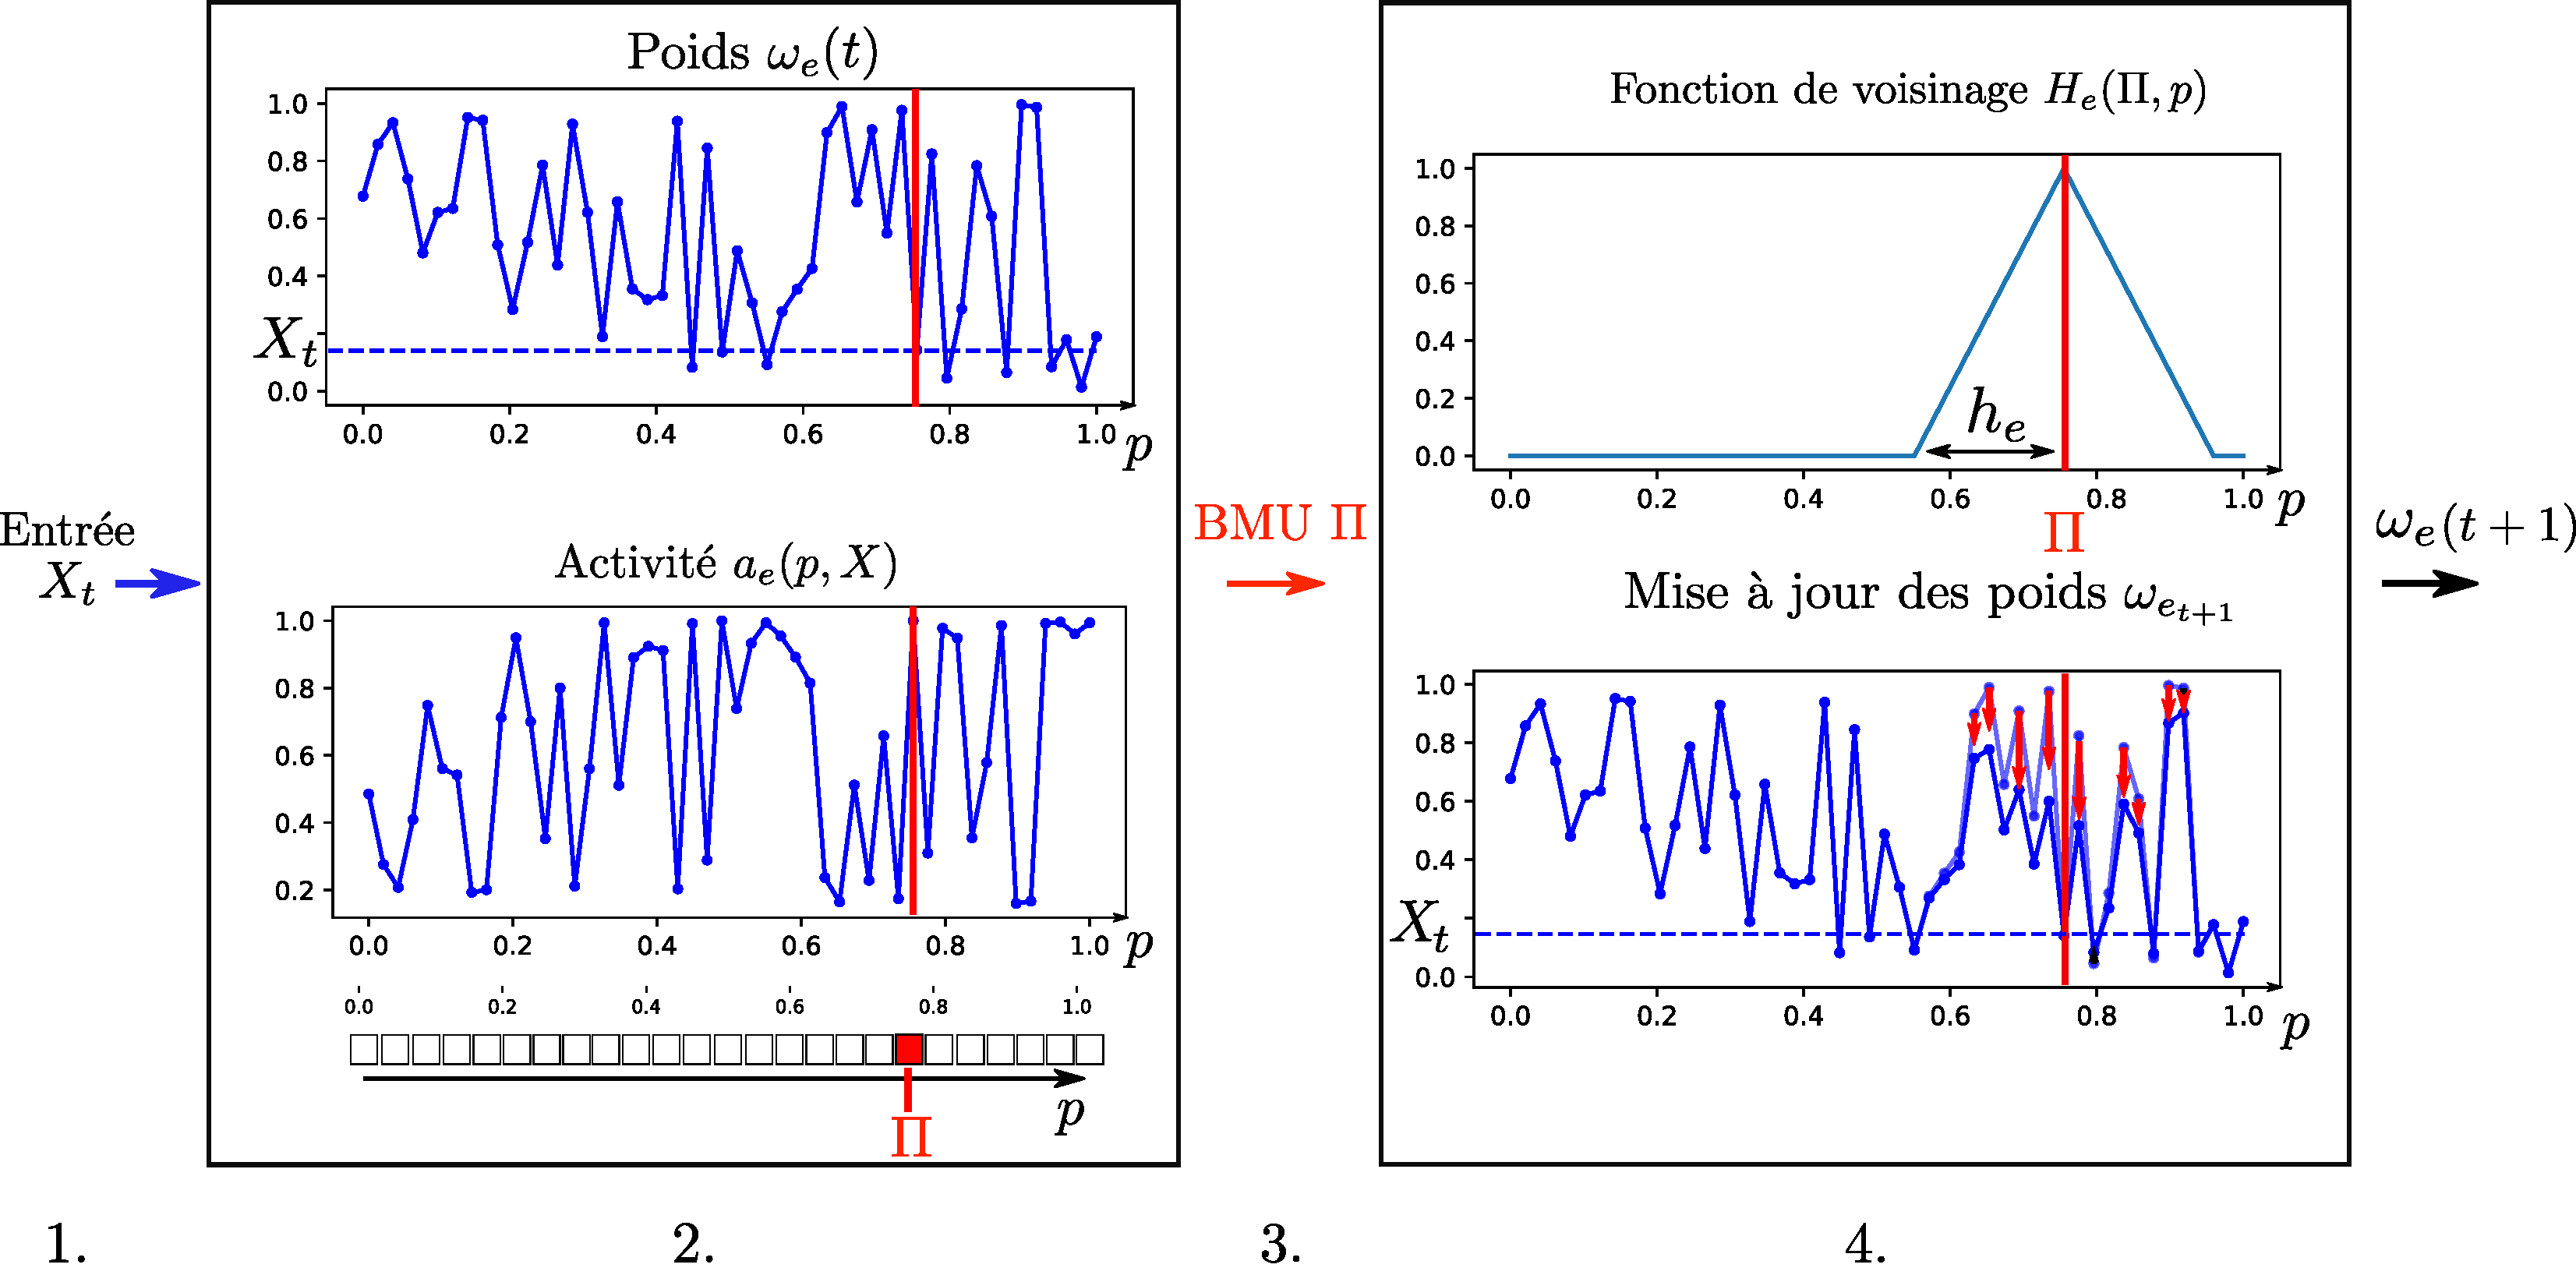
\includegraphics[width=\textwidth]{one_map_one_layer2.pdf}
\caption{Notations utilisées dans une carte de Kohonen simple. Les 4 étapes d'une itération d'apprentissage sont présentées: 1. Présentation de l'entrée, 2. Calcul de l'activité, 3. Choix du BMU, 4. Mise à jour des poids. \label{fig:one_map_not}}
\end{figure}

\subsection{Paramètrage d'une carte de Kohonen}\label{sec:parametres_carte}

L'organisation d'une carte de Kohonen est gérée par plusieurs paramètres, que nous présentons ici.
Les paramètres supplémentaires introduits par la version CxSOM sont présentés en partie \ref{sec:params}.

\subsubsection{Taux d'apprentissage $\alpha$}

Le taux d'apprentissage $\alpha$ détermine la proportion dans laquelle chaque poids est déplacé vers l'entrée lors de sa mise à jour, selon l'équation~\ref{eq:update}. 
Dans l'algorithme classique, le taux d'apprentissage décroît au cours de l'apprentissage. Au début de l'apprentissage, $\alpha$ est élevé, ce qui assure un dépliement rapide de la carte. La décroissance du taux d'apprentissage accompagne ensuite la convergence des poids de la carte au cours de l'apprentissage.

Un objectif à long terme de développement de l'architecture CxSOM est de construire des systèmes de cartes autonomes dynamiques. Ces systèmes apprennent sur des données en ligne, présentées séquentiellement et ayant des dépendances temporelles. Dans ce cas d'utilisation, il n'est pas souhaitable de faire décroître le taux d'apprentissage qui introduit un début et une fin d'apprentissage fixés par avance. Le calcul d'une itération dépend alors non seulement de l'état précédent de la carte, mais aussi de l'itération $t$ courante. 
Nous choisissons ainsi de garder un $\alpha$ constant dans le modèle CxSOM.
Les calculs réalisés lors d'une itération $t$ dépendent alors uniquement de l'état de la carte au pas de temps précédent.

\subsubsection{Topologie de la carte}

Une carte de Kohonen peut présenter des topologies diverses, comme détaillé en section~\ref{sec:som001}~: grilles, lignes, arbres, graphes \dots Les notations et l'algorithme CxSOM que nous présentons dans ce chapitre sont applicables à toutes les topologies de cartes. Dans cette thèse, nous nous concentrons sur des lignes 1D et des grilles 2D. Ce choix est d'abord motivé par le fait que les lignes et les grilles sont les formats de cartes les plus courants rencontrés dans la littérature. On parle souvent de cartes de Kohonen 1D et cartes 2D, en sous-entendant leur format de ligne ou de grille.

Ensuite, la spécificité des cartes de Kohonen tient à l'organisation des prototypes de façon continue. Lorsqu'on parle de continuité des prototypes dans une carte de Kohonen, il s'agit d'abord d'une relation de proximité et d'ordre entre des prototypes discrets: si deux unités sont proches dans la carte, alors leurs prototypes sont proches dans l'espace d'entrée. Un exemple d'organisation des poids d'une SOM en ligne 1D sur des données dans $[0,1]$ est tracé en figure~\ref{fig:depliement}. Les prototypes sont répartis aléatoirement dans l'espace d'entrée $[0,1]$ à l'itération $0$~; au cours de l'apprentissage, ils s'organisent de façon ordonnée. \`A partir de l'itération 500, on observe cette continuité des prototypes.

Le format particulier de ligne et de grille d'une carte de Kohonen permet d'étendre cette notion de proximité entre prototypes à une continuité des poids au sens mathématique, par interpolation. Dans ces formats 1D et 2D, l'ensemble des n\oe{}uds et de leurs arêtes est inclus dans une ligne ou un plan~: chaque arête de la grille peut être vue comme un ensemble de positions. Les poids de la carte sont dans ce cas une approximation discrète d'une fonction continue $\widetilde{\w_e}$, à valeurs dans~$\mathcal{D}$.
\begin{equation*}
\begin{array}{ccccc}
M& : & [0,1]^2 \; \text{ou} \;[0,1] & \to &  \mathcal{D} \\
 & & p & \mapsto & \widetilde{\w_e}(p) \\
\end{array}
\end{equation*}

Cette continuité est une des puissances d'une carte de Kohonen en tant qu'algorithme de quantification vectorielle. 
% Des opérations réalisées dans l'espace des positions $[0,1]$ correspondent directement à des opérations dans l'espace d'entrée $\mathcal{D}$, par la fonction $\widetilde{\w_e}$.

Au cours de l'apprentissage, les poids d'une carte se rapprochent de la distribution des données. On parlera de dépliement d'une carte lorsqu'on fait référence à son apprentissage.
Pour une carte 1D sur des données 1D, il est démontré en \cite{Cottrell1998TheoreticalAO} que les poids évolueront au cours de l'apprentissage vers un ordre strictement croissant ou strictement décroissant~; ordre qui ne sera plus modifié une fois atteint. 
Lorsque la dimension des données est plus grande que celle de la carte, par exemple des points 2D ou des images, la carte formera des plis de manière à remplir l'espace $\mathcal{D}$ (voir figure~\ref{fig:som1d}, section~\ref{sec:som001}). 

\begin{figure}
\centering
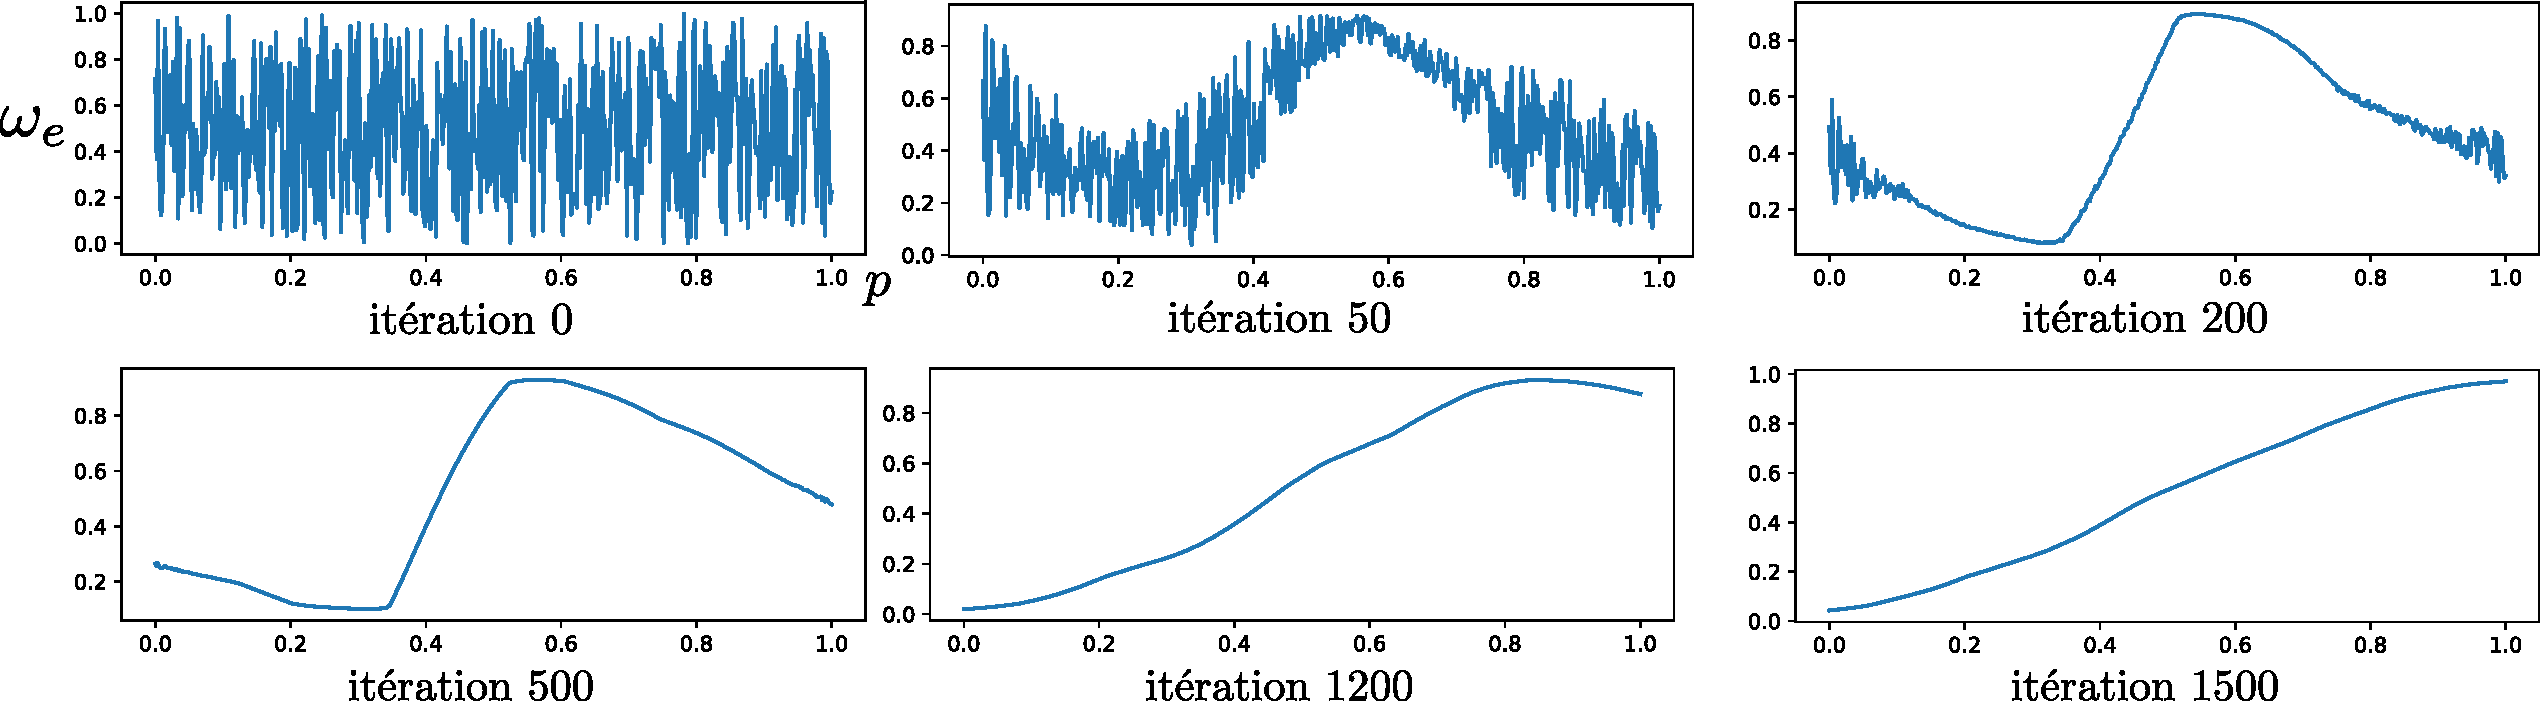
\includegraphics[width=\textwidth]{depliement_1D.pdf}
\caption{Exemple de dépliement d'une carte 1D de taille 500, sur des données 1D $\inpx \in [0,1]$. Les paramètres $h\ext = 0.2, \: \alpha = 0.2$ ont été gardés constants dans cet exemple. On s'attend à ce que les poids de la carte soient organisés selon un ordre strictement croissant ou décroissant à la fin de l'apprentissage.}
\label{fig:depliement}
\end{figure}

\subsubsection{Rayon de voisinage}

Le rayon de voisinage $h_e$ détermine l'élasticité d'une carte en définissant quelles unités voisines du BMU auront leurs poids mis à jour.
Plus le rayon $h_e$ est grand, plus la partie de la carte dont les poids sont déplacés vers l'entrée lors de la mise à jour est étendue. 

Une carte ayant un grand rayon de voisinage est moins sensible aux variations locales des données et parvient à se déplier selon les variations à grande échelle de la distribution des entrées.
Un petit rayon d'apprentissage permet au contraire de déplacer les poids concentrés dans une petite région sans affecter toute la carte. Les poids s'ajustent ainsi aux variations locales des entrées. Par contre, choisir un rayon de voisinage petit dès le début de l'apprentissage empêche la carte de se déplier globalement de façon ordonnée. Elle se divisera en morceaux ordonnés séparément~\parencite{Kohonen1995SelfOrganizingM}.
Le choix de l'élasticité est donc un compromis entre apprentissage d'une structure globale des entrées et ajustement aux variations locales.
Dans l'algorithme classique, ce compromis est trouvé en faisant décroitre le rayon de voisinage au cours de l'apprentissage. Un grand rayon de voisinage permet à la carte de se déplier rapidement en apprenant une structure globale des données. Sa décroissance au cours des itérations permet d'affiner l'apprentissage des données à un niveau plus fin. 
Contrairement à la plupart des SOM classiques, nous garderons des rayons de voisinage constants dans CxSOM. Tout comme le fait de garder le taux d'apprentissage constant, garder le rayon de voisinage constant est motivé par les objectifs de traitement de données séquentielles, vers des systèmes de cartes utilisés en continu.

\section{Motivations du modèle CxSOM}

\`A partir du modèle de carte de Kohonen détaillé en section \ref{sec:kohonen}, nous proposons un modèle de carte auto-organisatrice servant de module de base pour construire des architectures non-hiérarchiques. 
Nous présentons tout d'abord les choix de développement effectués pour créer le modèle d'architecture.

\subsection{Champ d'application: mémoire associative}

Dans cette thèse, nous étudions les capacités d'une architecture à apprendre des relations entre des entrées non temporelles. 
On considère un ensemble d'espaces d'entrée $\mathcal{D}\m{1}, \cdots , \mathcal{D}\m{n}$, appelés modalités.
Les entrées présentées à une architecture de cartes sont $(\inpx\m{1}_t, \cdots, \inpx\m{n}_t) \in \mathcal{D}\m{1} \times \cdots \times \mathcal{D}\m{n}$. 
On se place dans un cadre où les distributions des modalités considérées $\inpx\m{i}$ dépendent les unes des autres.
Lorsqu'on tire une entrée pour la présenter à une carte, on tire une entrée jointe $\mathbf{\inpx} =  (\inpx\m{1}_t, \cdots , \inpx\m{n}_t)$, dont chaque composante est présentée à la carte qui lui correspond. 
Le but pour l'architecture de cartes est d'encoder une représentation de chaque espace d'entrée $\mathcal{D}\m{i}$ et d'encoder le schéma de dépendances entre modalités au sein de l'architecture, ce que nous appelerons mémoire associative.
La figure~\ref{fig:input_3som} présente deux exemples de disposition jouet en 2D et 3D. Les modalités sont chacune des coordonnées, et le but de la mémoire associative est d'apprendre les relations entre modalités, c'est-à-dire détecter qu'elles sont disposées sur un cercle.

\begin{figure}
\centering
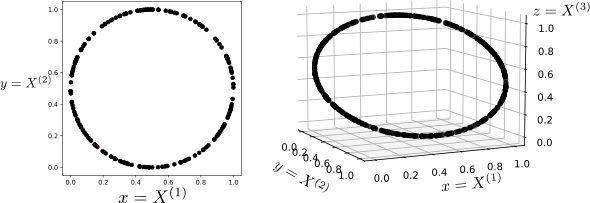
\includegraphics[width=\textwidth]{inputs_3som}
\caption{Exemple de disposition d'entrées en deux dimensions, à gauche, et trois dimensions, à droite. Les modalités associées à différentes cartes sont les coordonnées $x,y$ et $z$ de chaque point. Dans une telle disposition, les modalités dépendent les unes des autres~: développer une mémoire associative signifie apprendre le modèle de relation existant etre $x,y$ et $z$, c'est-à-dire le cercle.\label{fig:input_3som}}
\end{figure}

\subsection{Description de l'architecture}

Nous avons souligné les différents types d'interfaces entre cartes dans une architecture au chapitre~\ref{chap:architectures}.
Dans CxSOM, on choisit de se placer dans le paradigme de transmission de la position du BMU entre cartes: on connecte une carte B à une carte A en donnant la position du BMU de B en entrée à la carte A. 
Contrairement aux cartes hiérarchiques comme HSOM~\parencite{lampinen_clustering_1992} dans lesquelles la position du BMU est la seule entrée d'une carte de plus haut niveau, chaque carte de l'architecture peut posséder une entrée principale propre issue d'une modalité $\inpx\m{i}$ que nous appelons l'entrée externe. 
Une carte prendra également un ensemble d'entrées secondaires qui sont les positions des BMU des autres cartes de l'architecture. 
% Les cartes auto-organisatrices dans le modèle CxSOM prennent donc un nombre arbitraire d'entrées, dont certaines sont les BMU d'autres cartes. On appelle ces entrées internes à l'architecture les entrées \emph{contextuelles} d'une carte.
% L'algorithme d'apprentissage d'une carte auto-organisatrice prenant une position de BMU en tant que contexte est similaire à celui d'une carte classique, comprenant:
% \begin{enumerate}
% \item\label{etape:entree} Présentation des entrées externes et contextuelles à chaque carte 
% \item\label{etape:bmu} Recherche du BMU par calcul d'activité
% \item\label{etape:maj} Mise à jour des poids selon une fonction de voisinage
% \end{enumerate}
% Chaque carte aura simplement plusieurs entrées: une entrée \emph{externe} dans un espace d'entrée, et $k$ entrées \emph{contextuelles} qui sont les positions des BMU des cartes qui lui sont connectées. 
Une carte peut ne prendre que des entrées contextuelles.
La recherche du BMU doit être modifiée par rapport à la méthode originale~: les rétroactions entre les cartes étant autorisées, la position du BMU de la carte A va donc influencer la position du BMU de la carte B, laquelle modifie à nouveau le BMU de la carte A, etc. 

Notre algorithme implémente deux modifications principales par rapport à l'algorithme d'apprentissage d'une carte de Kohonen classique: 
\begin{itemize}
\item Les cartes possèdent plusieurs entrées, externes et contextuelles; les entrées contextuelles sont les positions des BMU d'autres cartes. Le calcul de l'activité est modifié afin de prendre en compte cet ensemble d'entrées.
\item La recherche du BMU est modifiée afin de gérer les rétroactions entre cartes.
\end{itemize}

L'architecture CxSOM couple ainsi l'apprentissage de plusieurs cartes. Chaque carte apprend à la fois ses entrée $\inpx\m{i}$, mais aussi un contexte avec les BMU des autres cartes.
Seule la position du BMU est utilisée comme information transmise entre carte. Cette valeur apporte une homogénéité dans l'architecture de cartes~: quelles que soient les entrées d'une carte et leurs dimensions, le BMU sera une position en 1 ou 2 dimensions. De plus, transmettre seulement la position du BMU est une avantage en terme de quantité d'information à transmettre.
Nous laissons aussi la possibilité d'utiliser des cartes ne prenant que des entrées contextuelles. Ces cartes agissent alors comme des cartes intermédaires, connectant des cartes prenant des entrées externes.

\section{Présentation de CxSOM: exemple d'une architecture de deux cartes}

Présentons le fonctionnement d'une architecture simple~: deux cartes $M\m{1}$ et $M\m{2}$, connectées réciproquement, présentée en figure~\ref{fig:2som_archi}. Toutes les équations seront ensuite formalisées dans le cas général en section~\ref{sec:formalisme}. 
Nous prenons dans cet exemple des cartes en une dimension, indexées par $p \in [0,1]$.
\begin{figure}[ht]
    \centering
    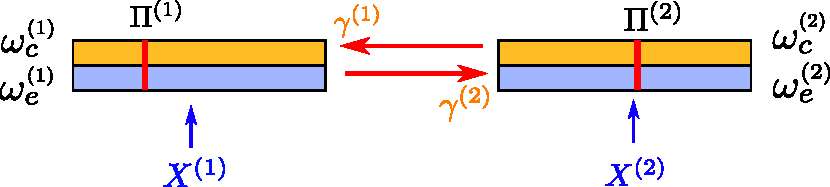
\includegraphics[width=0.7\textwidth]{archi_2som}
    \caption{Architecture de deux cartes. Chaque carte possède deux couches de poids, relatives à l'entrée externe $\inpx\m{i}$ et à l'entrée contextuelle $\inpc\m{i}$.
    Ces entrées contextuelles correspondent à la position du BMU de l'autre carte à l'issue du processus dynamique de recherche du BMU par relaxation.
    \label{fig:2som_archi}}
    \end{figure}
\subsection{Détail des étapes}

\paragraph{Structure d'une carte}
\begin{figure}
    \centering
    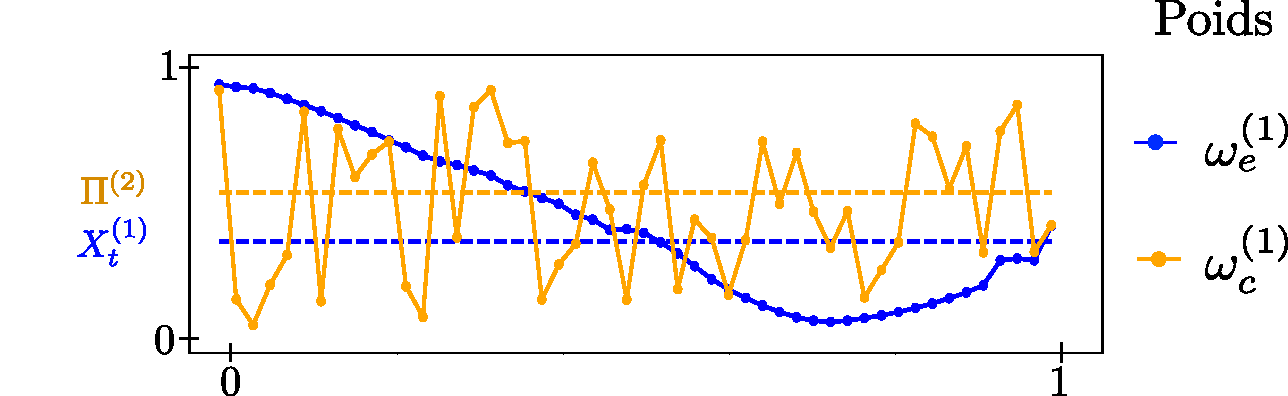
\includegraphics[width=0.75\textwidth]{weights_2som.pdf}
    \caption{Représentation des poids de $M\m{1}$. L'entrée externe $\inpx_t\m{1}$ présentée à l'itération $t$, tirée d'un espace d'entrée 1D $[0,1]$, est indiquée en bleu sur le graphique. L'entrée contextuelle $\inpc\m{1}$ est le BMU de la carte $M\m{2}$. Sa valeur est indiquée en jaune; il s'agit d'une position 1D dans la carte $M\m{2}$, à valeur entre 0 et 1. \label{fig:2som_weights}}
    \end{figure}
Chaque carte $M\m{i}$ de l'architecture prend une entrée externe, $\inpx\m{i}$ et une entrée contextuelle $\inpc\m{i}$. Il s'agira de la position courante du BMU de l'autre carte.
Les entrées externes $\inpx\m{1}_t$ et $\inpx\m{2}_t$ sont deux modalités interdépendantes.
Les élements des cartes sont indicés par $(1)$ et $(2)$ pour désigner les éléments appartenant à la carte $M\m{1}$ et $M\m{2}$.
Une carte $i$ ($i \in \{1,2\}$) possède deux couches de poids, chacune étant relative à une entrée~: les poids \emph{externes} $\w_e\m{i}$, qui se déplient sur les entrées $\inpx\m{i}$, et les poids contextuels $w_c\m{i}$, qui se déplient sur les entrées contextuelles, qui appartiennent à l'espace des positions en une dimension de l'autre carte. 
Ces deux couches de poids sont représentées en figure~\ref{fig:2som_weights}. 
% La position du BMU de $M\m{2}$, $\bmu\m{2}_t$ est utilisée comme entrée contextuelle $\inpc\m{1}$ de $M\m{1}$, et $\bmu\m{1}_t$ comme entrée contextuelle de $M\m{2}$.

\paragraph{Calcul d'activité}

Chaque carte calcule une activité sur chaque entrée externe et contextuelle et les combine en une activité globale permettant de calculer un BMU commun à toutes les couches de poids de la carte.
Les activités externes et contextuelles sont calculées par une activation gaussienne, cf. équation~\ref{eq:act1som} et tracées en figure~\ref{fig:2som_activite}.
Pour la carte $M\m{1}$, au pas de temps $t$, on a ainsi~:
\begin{equation}
\label{eq:activite}
\begin{cases}
a_e\m{1}(p, \inpx\m{1}) = \exp\frac{-\lVert \w_e\m{1}(p)-\inpx\m{1}_t \rVert^2}{2\sigma^2} \\
a_c\m{1}(p, \inpc\m{1}) = \exp\frac{-\lVert \w_c\m{1}(p)-\inpc\m{1} \rVert ^2}{2\sigma^2}\\
\end{cases}
\end{equation}

$a_c$ et $a_e$ sont ensuites combinées en une activité globale~:
\begin{equation}
a_g\m{1}(p, \inpx\m{1}_t,\inpc\m{1}) = \sqrt{a_e(p, \inpx\m{1}_t)\times \frac{a_e(p, \inpx\m{1}_t) + a_c(p,\inpc\m{1})}{2}}
\end{equation}

Par la différence de contribution de $a_c$ et $a_e$ au sein de l'activité globale -- $a_c$ ne contribue qu'à la puissance $\frac{1}{2}$ -- on assure que l'activité contextuelle vient seulement moduler l'activité externe.
On peut observer cette modulation sur la courbe noire de la figure~\ref{fig:2som_activite}~: l'activité globale suit la même progression que l'activité externe, mais est modifiée localement par les variations de l'activité contextuelle. 
De cette façon, les entrées contextuelles ne viennent pas donner d'\og hallucinations \fg{} à la carte~: elle apprend en priorité ses entrées externes, conditionnées aux entrées contextuelles. Ce choix de combinaison des activités est issu du modèle de cartes cellulaires Bijama développé au sein de notre équipe \parencite{menard05,khouzam_2013,baheux_towards_2014}.

\begin{figure}
    \centering
    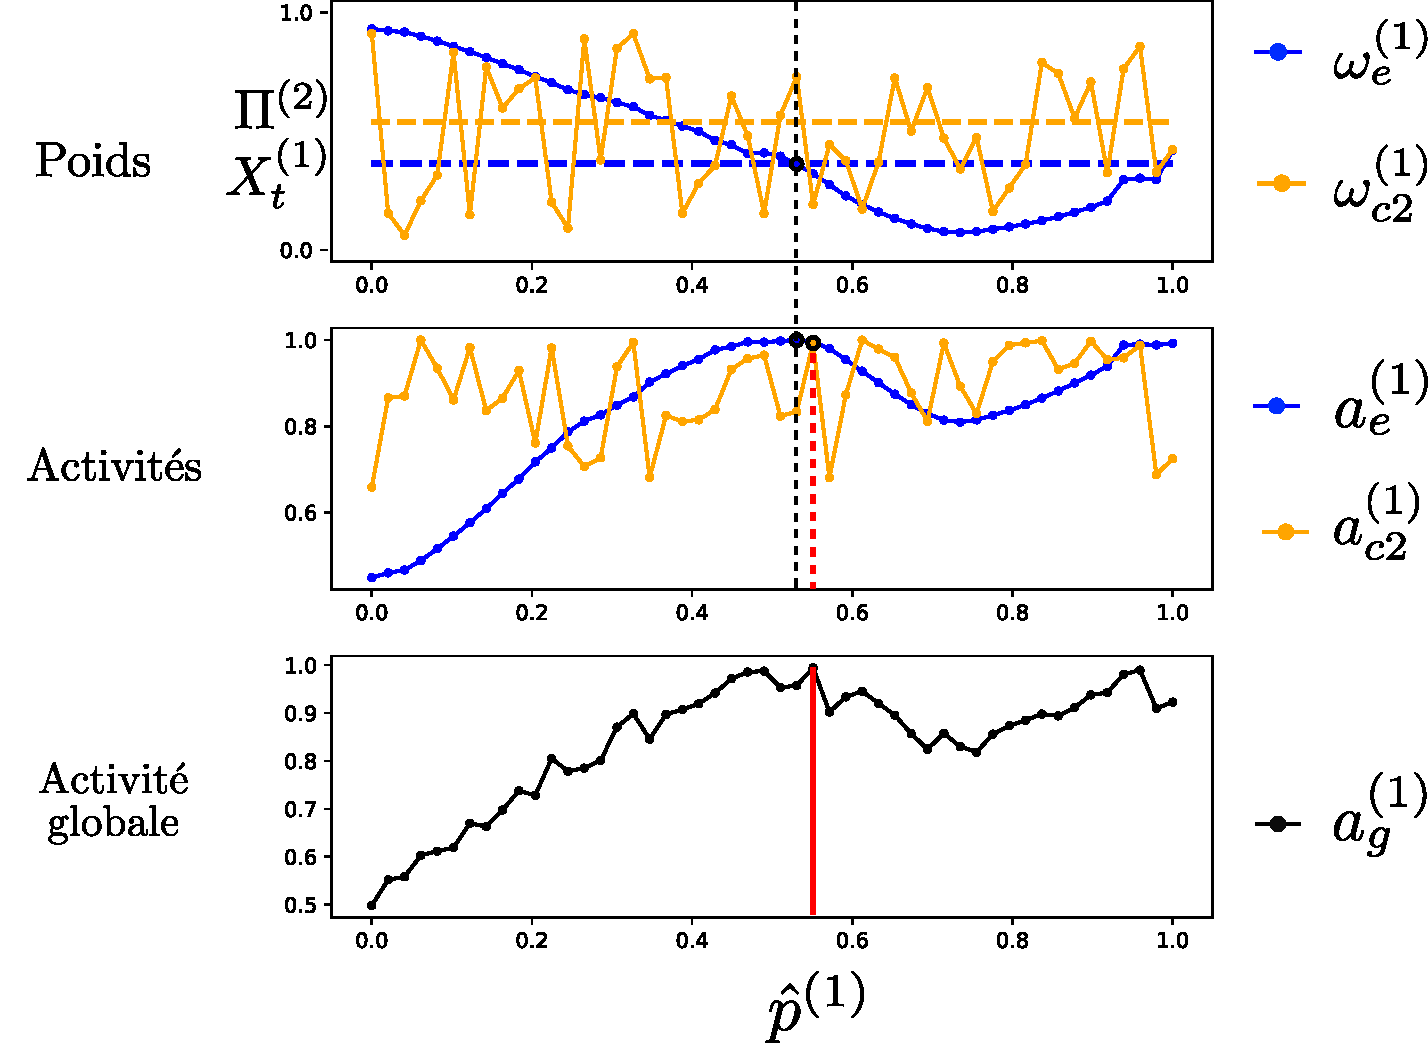
\includegraphics[width=0.7\textwidth]{activite_layers_2maps.pdf}
    \caption{Calcul d'activité dans une SOM au sein d'une architecture de deux cartes. La carte prend une entrée externe et une entrée contextuelle. 
    L'entrée externe est $X\m{1}_t$. La carte possède deux couches de poids, permettant de calculer deux activités. L'activité globale prend en compte toutes les couches d'activités afin de trouver un BMU commun à toutes les couches de poids. Le calcul de l'activité globale favorise l'activité externe et est modulé par l'activité contextuelle, ce qu'on observe sur la courbe du bas~: l'activité globale suit les variations de l'activité externe, et est localement modifiée par les variations de l'activité contextuelle.
    Le maximum de l'activité globale est noté $\hat{p}$. \`A partir de l'activité globale, le BMU $\bmu\m{1}_t$ sera trouvé par le processus de relaxation. \label{fig:2som_activite}}
    \end{figure}

\paragraph{Relaxation}\label{sec:relax}
\begin{figure}
    \centering
    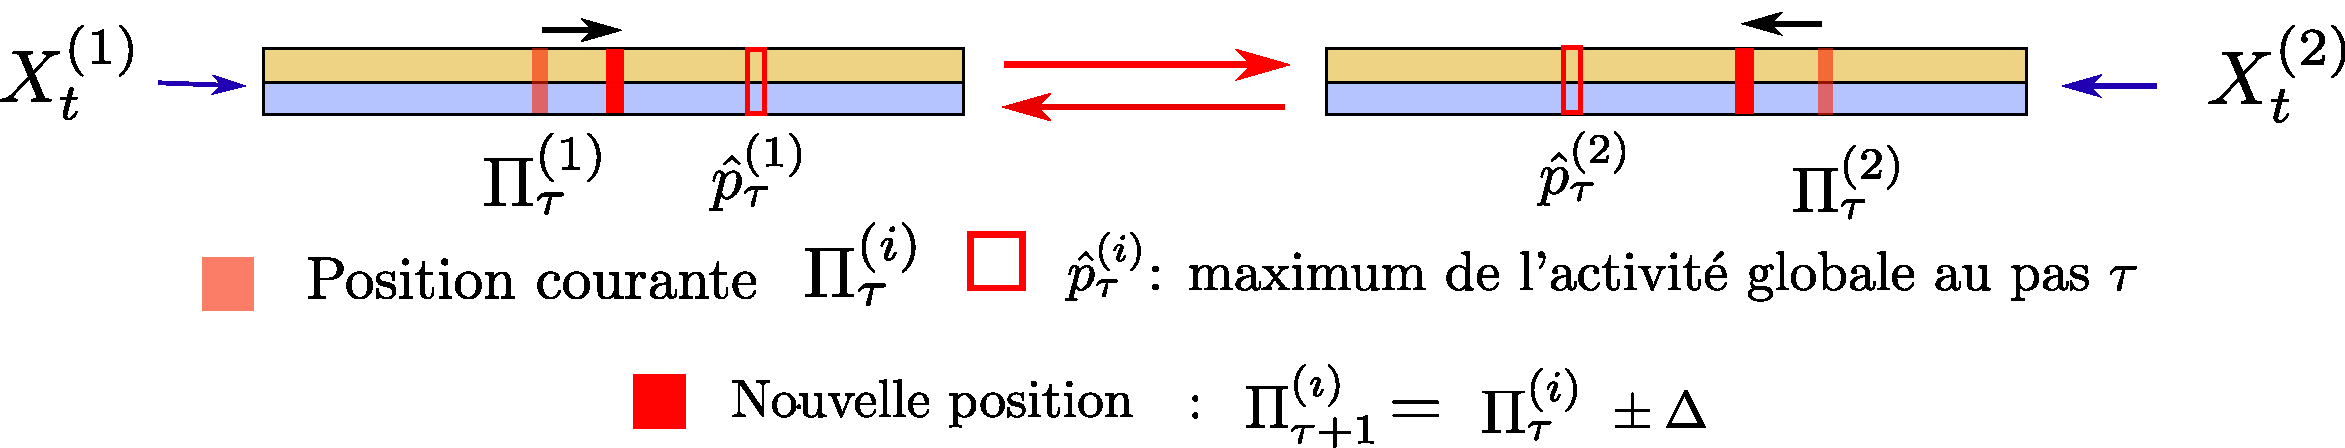
\includegraphics[width=\textwidth]{relaxation_2maps.pdf}
    \caption{Description d'une étape de relaxation dans l'architecture, aboutissant à un consensus entre cartes. Lors de la relaxation, les positions $\bmu_\tau$ sont légèrement déplacées jusqu'à ce que toutes les positions $\bmu_\tau$ des cartes de l'architecture soient stables. Ce point de convergence correspond à un ensemble de positions qui maximise l'activité de chaque carte. \label{fig:relax}}
    \end{figure}

Nous voulons donner en entrées contextuelles $\gamma\m{1}$ d'une carte les positions du BMU $\bmu\m{2}_t$.
Contrairement à une carte simple, on ne peut pas calculer tous les BMU de l'architecture chacun leur tour~: le calcul du BMU de $M\m{1}$ influence l'activation de $M\m{2}$ et donc son BMU, qui modifie le BMU de $M\m{1}$.
Nous remplaçons donc l'étape de simple calcul d'argmax d'une carte classique par un processus de recherchee de BMU global à l'architecture. Cette recherche est réalisée par un processus dynamique que l'on appelera \emph{relaxation}, menant à un \emph{consensus} entre cartes~: on cherche un point, s'il existe, où le BMU dans chaque carte est au plus proche du maximum de son activité globale $\hat{p}\m{i} = \argmax\limits_p a_g\m{i}(p, X\m{i}, \gamma\m{i})$.

Cette recherche est réalisée par une sous-boucle incluse dans un pas d'apprentissage $t$, indexée par $\tau$. Cette sous-boucle définit une suite de positions intermédaires, $(\bmu\m{1}_\tau , \bmu\m{2}_\tau)$, permettant de chercher le BMU itérativement.
Le processus de relaxation est le suivant~:
\begin{enumerate}
\item Les entrées externes sont présentées au début de la boucle, donc $a_e$ peut être calculée; $\bmu\m{1}_0$ et $\bmu\m{2}_0$ sont initialisées à la position où les activités externes sont maximales dans chaque carte. 
\item Tant que la suite de positions $(\bmu\m{1}_\tau,\bmu\m{2}_\tau)$ n'a pas convergé:
	\begin{enumerate}
	\item Dans chaque carte, nous calculons les activités contextuelles et globales, définissant ainsi $\hat{p}\m{1}_\tau = \argmax\limits_p(a_g\m{1}(p,\inpx\m{1}, \bmu\m{2}_\tau)$, de même pour $\hat{p}\m{2}$.
	\item Nous déplaçons $\bmu\m{1}$ vers $\hat{p}\m{1}$ et $\bmu\m{2}_\tau$ vers $\hat{p}\m{2}$ d'un pas $\Delta$: $\bmu\m{1}_{\tau+1} = \bmu\m{1}_{\tau} \pm \Delta$.
	Si une des valeurs est plus proche de $\hat{p}$ que $\Delta$, on déplacera $\bmu_\tau$ directement sur $\hat{p}$ pour éviter les oscillations autour du point. Cette étape est illustrée en figure~\ref{fig:relax}.
	\end{enumerate}
\item Le BMU de chaque carte est pris comme la valeur finale stable de ce processus dynamique. On note cette position finale $\bmu\m{i}_t$.
Si la relaxation n'atteint pas de point stable, nous fixons un nombre d'itérations maximum $\tau_{max}$ après lequel on arrête la relaxation.
\end{enumerate}

\paragraph{Mise à jour}
\begin{figure}
    \centering
    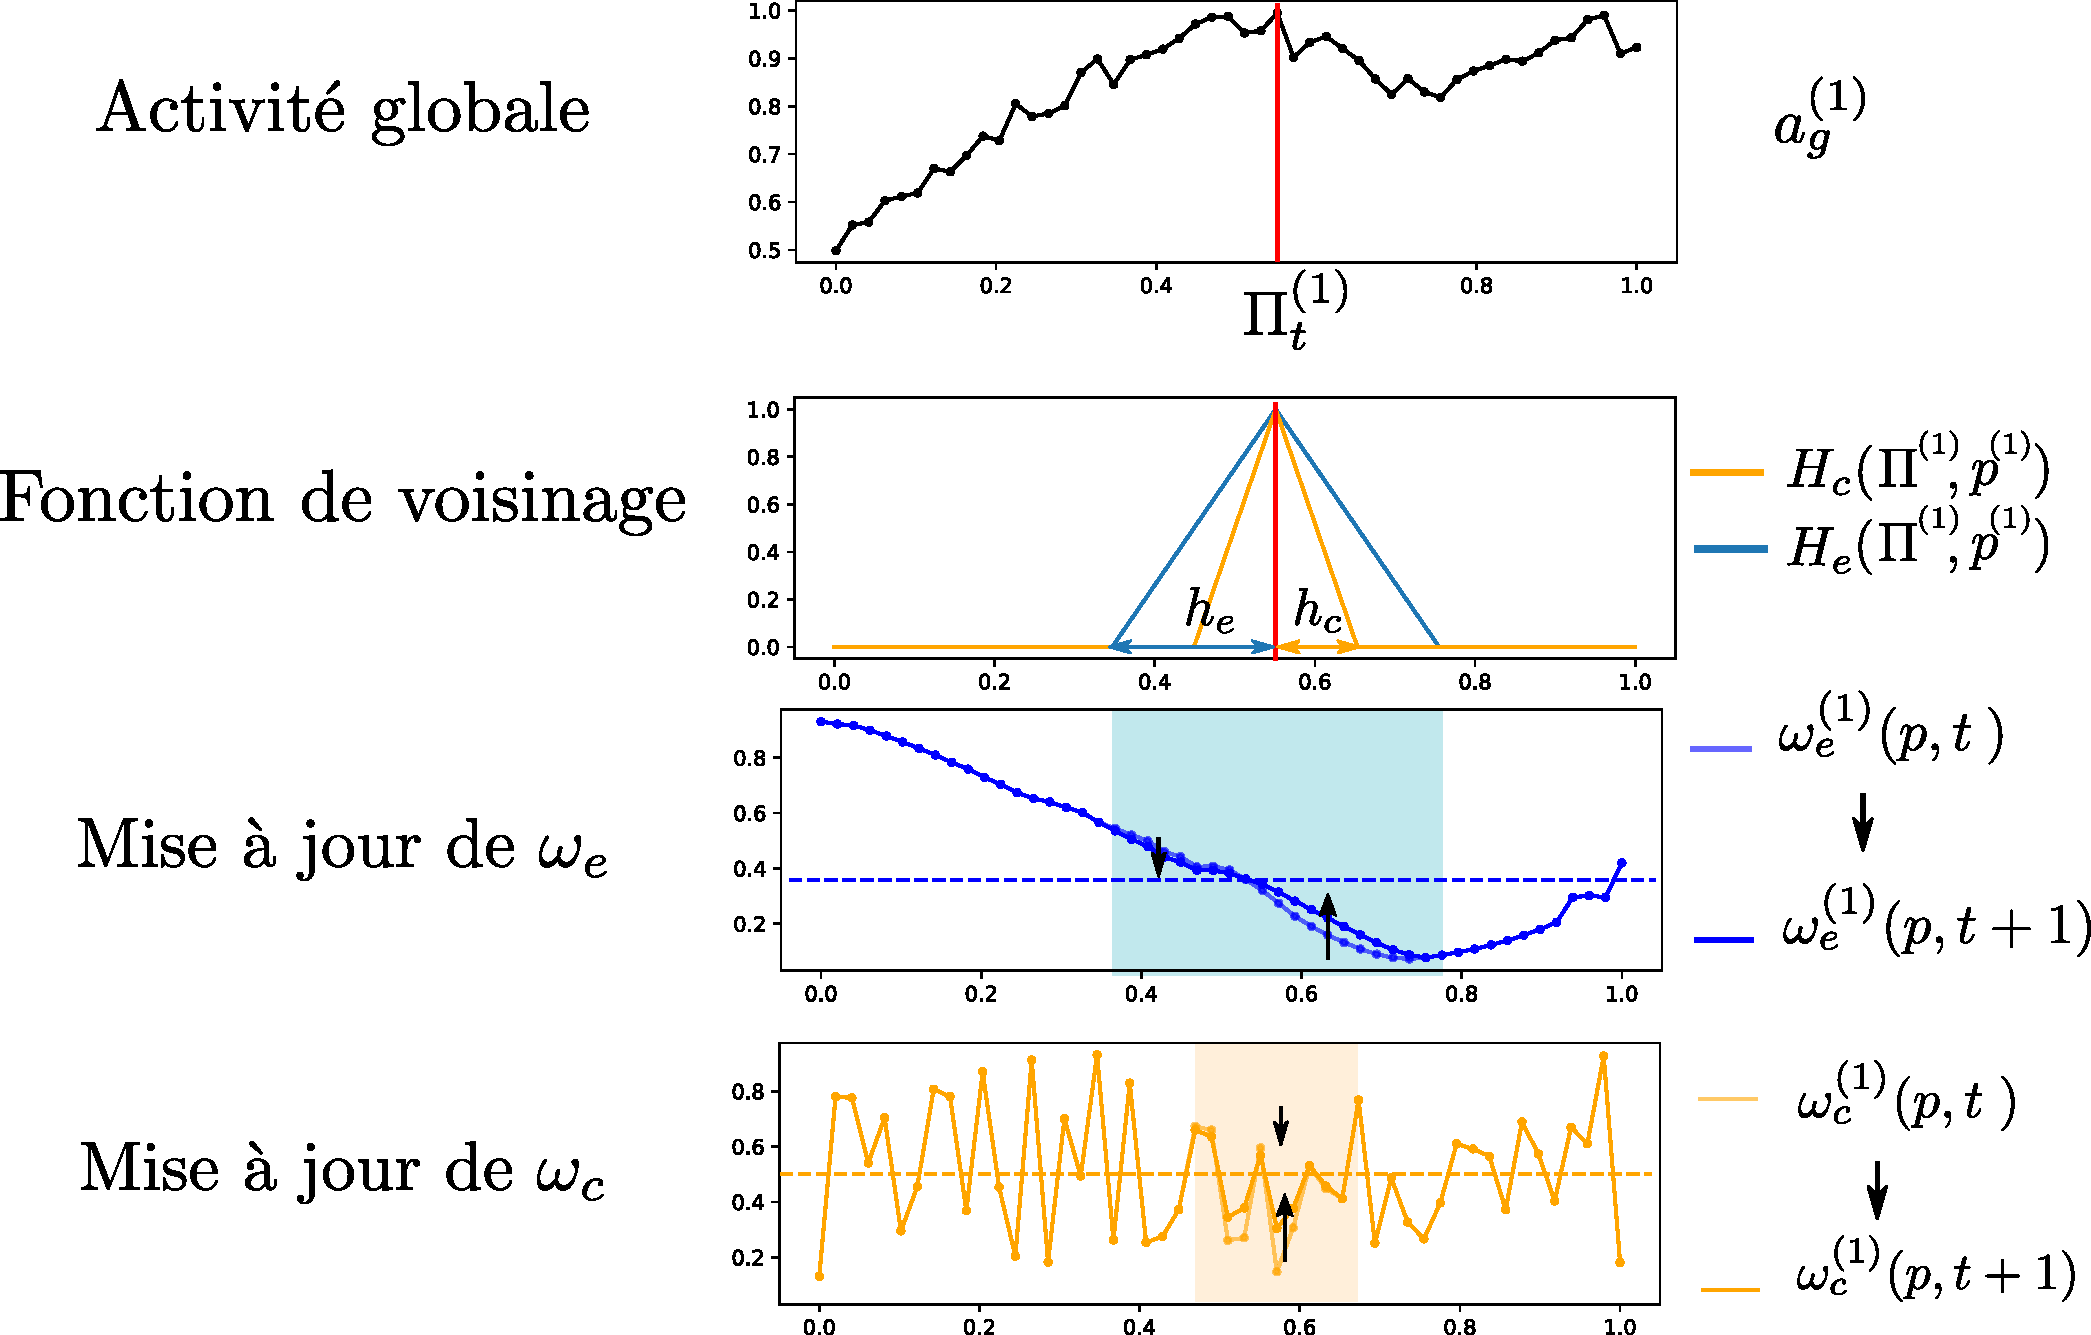
\includegraphics[width=0.7\textwidth]{maj_2som.pdf}
    \caption{Mise à jour de chaque couche de poids indépendamment, relativement au BMU commun à toutes les couches $\bmu\m{1}_t$, calculé par relaxation. Si la relaxation a convergé, la position $\bmu\m{1}_t$ est à la position $\hat{p}\m{1}$ maximisant l'activité globale à la fin de la relaxation. Le rayon de voisinage $h_e$ est utilisé pour mettre à jour les poids externes, le rayon $h_c$ pour mettre à jour les poids contextuels. On choisit $h_e > h_c$.
    Ce choix sera détaillé dans les chapitres suivants.\label{fig:maj}}
    \end{figure}

Dans chaque carte, chaque couche de poids $\w\ext\m{i}$, $\w_c\m{i}$ est mise à jour indépendamment dans chaque carte selon l'équation~\ref{eq:update}. La mise à jour dépend du BMU $\bmu\m{i}_t$, des entrées externes $\inpx\m{i}_t$ et contextuelles $\gamma\m{i} = \bmu\m{j}_t$ ($j \neq i$). 
Cette mise à jour correspond à la figure~\ref{fig:maj}.
Notons que nous choisissons ici des rayons d'apprentissage différents entre couche externe et couche contextuelle~; nous détaillerons ce choix au cours des expériences.



\subsection{Résumé}
Les étapes d'un pas d'apprentissage $t$ d'une architecture de deux cartes sont les suivantes~; elles sont schématisées en figure~\ref{fig:algo}.
\begin{enumerate}
\item Présentation des entrées $\inpx\m{1}_t$ et $\inpx\m{2}_t$ à chaque carte
\item Relaxation~:
\begin{enumerate}
\item Calcul de l'activité externe $a_e(p, \inpx\m{i}_t)$ dans chaque carte et initialisation des BMU $(\bmu\m{1}_0,\bmu\m{2}_0)$ pour la relaxation.
\item Relaxation par petits déplacements de ($\bmu\m{1}_\tau,\bmu\m{2}_\tau$) dans chaque carte, avec calcul de l'activité contextuelle et globale à chaque pas $\tau$, jusqu'à une stabilisation du couple de valeurs $(\bmu\m{1}_\tau,\bmu\m{2}_\tau)$
\item Définition des positions des BMU $\bmu\m{1}_t$ et $\bmu\m{2}_t$ commes les valeurs de $\bmu\m{1}_\tau$ et $\bmu\m{2}_\tau$ à l'issue de la relaxation.
\end{enumerate}
\item Mise à jour des poids $\w\ext\m{i}$ et $\w\cont\m{i}$ dans chaque carte, selon sa position du BMU $\bmu\m{i}_t$, son entrée externe $\inpx\m{i}_t$ et son entrée contextuelle $ \inpc\m{i} = \bmu\m{j}_t$, avec $\bmu\m{j}_t$ la position du BMU calculée par relaxation dans l'autre carte.
\end{enumerate}

\begin{figure}
\centering
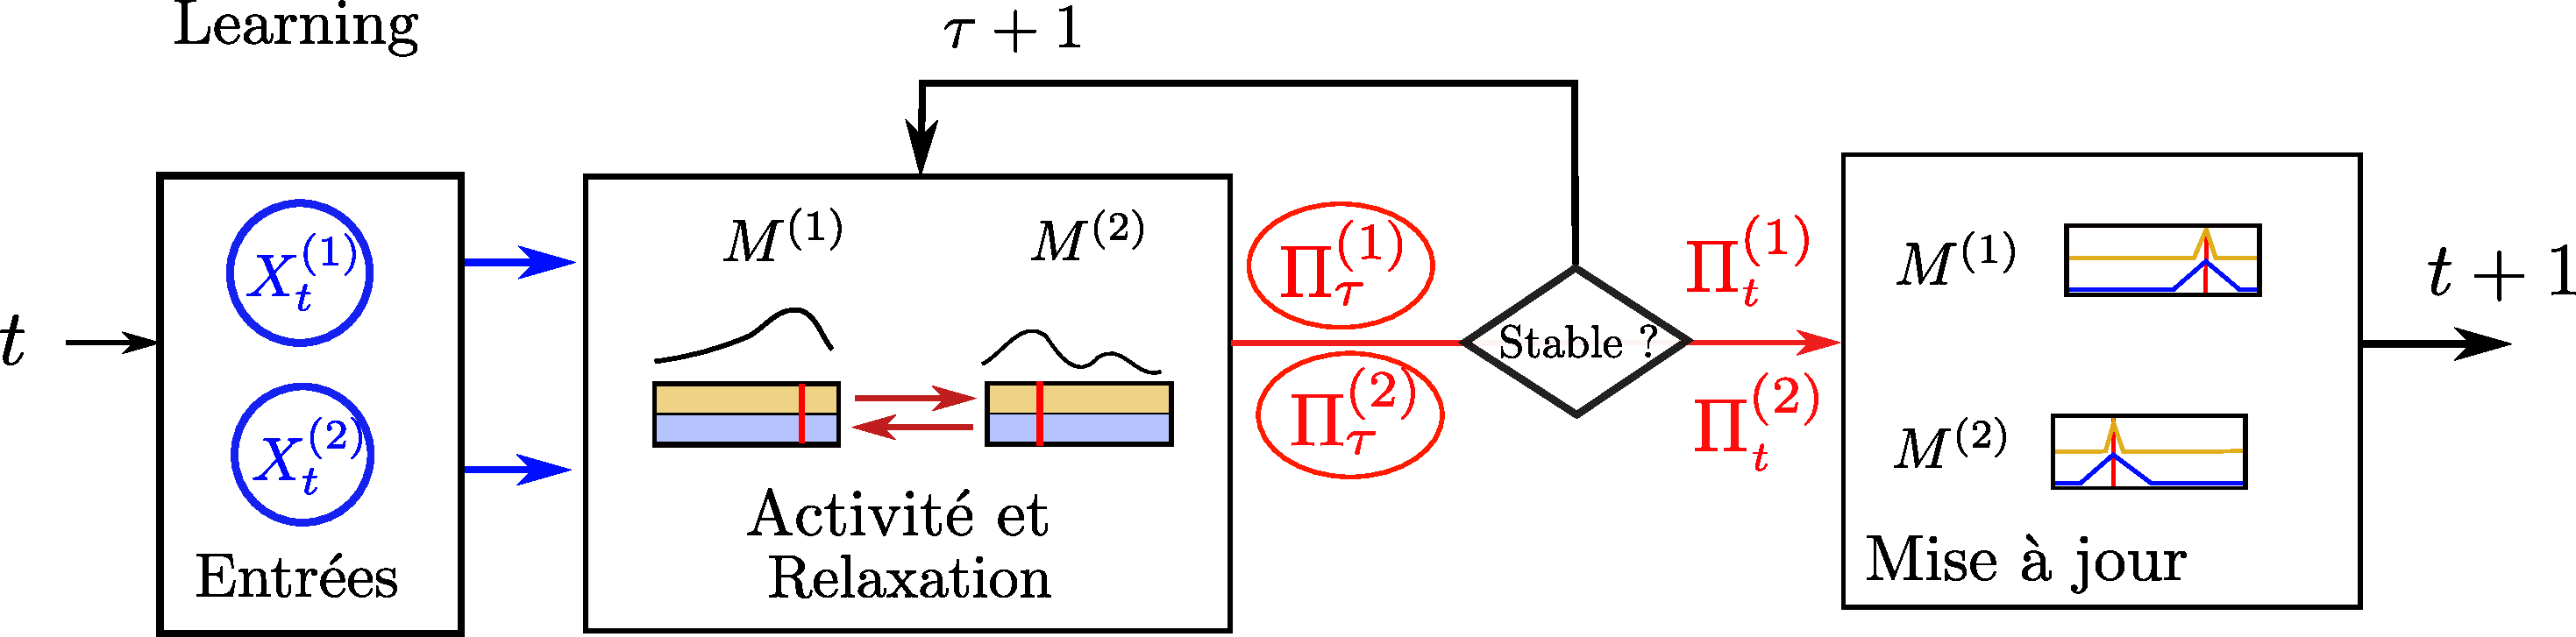
\includegraphics[width=\textwidth]{learning_tests_2maps}
\caption{Résumé des étapes de l'algorithme d'apprentissage d'une architecture, composé d'une boucle de recherche de BMU par relaxation dans laquelle les cartes sont couplées, puis d'une étape de mise à jour des différentes couches de poids séparément sur chaque carte.}
\label{fig:algo}
\end{figure}

\section{Formalisation: cas pour $n$ cartes}\label{sec:formalisme}

Nous présentons dans cette partie l'algorithme général pour une architecture quelconque de $n$ cartes. 
Les notations sont valables pour des cartes de dimension quelconque~; les entrées que nous avions illustrées par des valeurs 1D sont également de dimension quelconque.
La différence principale avec l'exemple à deux cartes est qu'une carte peut prendre plusieurs entrées contextuelles, qui sont les BMU de toutes les cartes qui lui sont connectées dans l'architecture, au lieu d'une seule dans le cas de l'exemple à deux cartes. On retrouvera donc les notations de la partie précédente.
Cette partie concentre toutes les notations et l'algorithme utilisé dans cette thèse. 
L'algorithme est résumé en algorithme~\ref{algo:cxsom}.

Dans une architecture composée de $n$ cartes, les cartes sont indexées par $i \in \{1,\cdots,n\}$. On indicera chaque élément d'une carte $M\m{i}$ par l'exposant $(i)$.
Pour faciliter la lecture, nous omettrons l'exposant $(i)$ dans les équations, lorsqu'on se concentre sur une seule carte. $\inpx_t$ désigne donc $\inpx_t\m{i}$, $\w_e$ désigne $\w_e\m{i}$, etc.

Lors d'un pas d'apprentissage $t$, une carte $M\m{i}$ reçoit en entrée une entrée \emph{externe} notée $\inpx_t$ et $K$ entrées \emph{contextuelles}. Notons-les $\Gamma = (\inpc{i_1},\cdots,\inpc{i_K})$~; elles seront les positions du BMU $\bmu\m{i_k}$ des cartes d'indice $i_k$ qui lui sont connectées, c'est-à-dire $\bmu\m{i_k}_\tau$ lors de la relaxation puis $\bmu\m{i_k}_t$ lors de la mise à jour.

La carte possède donc $K+1$ couches de poids. On note $\w_e(p)$ les poids externes et $\w_{ci_1}(p), \cdots, \w_{ci_K}(p)$ les poids correspondant aux entrées contextuelles, les \emph{poids contextuels}.
$\w_{ci_k}$ correspond à la couche de poids relative à l'entrée contextuelle $\inpc_{i_k}$. Les poids externes sont à valeurs dans $\mathcal{D}\m{i}$, la modalité associée à la carte $i$. Les poids contextuels sont à valeurs dans l'espace des positions d'une cartes, soit $[0,1]$ en 1D ou $[0,1]^2$ en 2D.

Les activités externes et contextuelles s'expriment de la façon suivante:
\begin{equation}
\label{eq:activite_general}
\begin{cases}
a_e(\inpx_t,p) = \exp\frac{-\lVert \w_e(p)-\inpx_t \rVert^2}{2\sigma^2} \\
a_{ci_k}(\inpc_{i_k},p) = \exp\frac{-\lVert \w_{ci_k}(p)-\inpc_{i_k} \rVert ^2}{2\sigma^2}, \\
\text{Avec $i_k$ les indices des cartes connectées à $i$}
\end{cases}
\end{equation}

Notons $a_c(p, \Gamma)$ la moyenne des activités contextuelles, avec $\Gamma = (\inpc_{i_1}, \cdots, \inpc_{i_K})$.
\begin{equation}\label{eq:ac}
a_c(p, \Gamma) = \frac{1}{K}\sum_{k=1}^K {a_{ci_k}(p,\inpc_{i_k})}
\end{equation}

L'activité globale $a_g$ est calculée en combinant l'activité externe et la moyenne des activités contextuelles~:
\begin{equation}
\label{eq:global_act}
a_g(p, \inpx_t,\Gamma) = \sqrt{a_e(p, \inpx_t) \frac{a_e(p, \inpx_t) +  a_c(p, \Gamma)}{2}}
\end{equation}

On notera également $\hat{p}$ la position du maximum de l'activité globale~:
\begin{equation}
\label{argmax}
\hat{p} = \argmax\limits_p a_g(p, \inpx_t, \Gamma)
\end{equation}

Notons qu'une carte peut ne pas avoir d'entrée externe. Dans ce cas, on prendra comme activité globale $a_c$, la moyenne des activités contextuelles (équation~\ref{eq:ac}).

% Dans chaque carte $i$, l'entrée contextuelle $\inpc\m{i}_{i_k}$ est le BMU à l'instant courant $\bmu\m{i_k}_t$  de la carte $k$. La position $\bmu\m{i}_t$ dépend donc des BMU des autres cartes, qui dépendent eux-mêmes de $\bmu\m{i}_t$. 
La relaxation est la recherche d'un ensemble de positions $\mathbf{\bmu}_t = (\bmu\m{1}_t, \cdots, \bmu\m{n}_t)$, si elles existent, telles que dans chaque carte, $\bmu\m{i}_t$ correspond à la position du maximum de l'activité globale, c'est-à-dire $\hat{p}\m{i}$.

\begin{equation}
\forall i, \; \bmu\m{i}_t = \argmax\limits_p a_g\m{i}(p, \inpx\m{i}_t, \inpc_0, \cdots, \inpc_K)
\end{equation}

Le processus de relaxation est une boucle imbriquée dans un pas d'apprentissage de l'architecture, indexée par $\tau$. Dans chaque carte, on construit une suite de positions $\bmu\m{i}_\tau$, dont la valeur finale sera le BMU $\bmu\m{i}_t$.
Lors d'une itération $t$, chaque carte est nourrie avec une entrée externe $\inpx\m{i}_t$ qui restera constante au cours de la relaxation. Les activités externes $a_e\m{i}(p, \inpx\m{i}_t)$ de chaque carte peuvent être calculées dès le début de la relaxation.
% La relaxation est définie comme suit~:
% \begin{enumerate}
% \item Dans chaque carte $i$, la position $\bmu\m{i}_0$ est initialisée à $\hat{p}\m{i}_0 = \argmax\limits_p a_e\m{i}(p, \inpx\m{i}_t)$.
% \item Dans chaque carte $i$, on assigne $\inpc_{i_k}\m{i} = \bmu\m{i_k}_\tau$
% \item Tant que toutes les positions $\bmu\m{i}$ n'ont pas atteint une valeur stable, c'est à dire, $\mathbf{\bmu}_{\tau+1} \neq \mathbf{\bmu}_\tau$:
% 	\begin{enumerate}
% 	\item Dans chaque carte $i$, calculer les activités contextuelles et globales, définissant ainsi $\hat{p}\m{i}_\tau = \argmax\limits_p a_g\m{i}(p,\inpx\m{i}, \bmu\m{i_0}_\tau,\cdots,\bmu\m{i_k}_\tau)$, avec $i_0, \cdots, i_k$ les indices des cartes connectées à $i$ dans l'architecture.
% 	\item Déplacer $\bmu\m{i}$ vers $\hat{p}\m{i}$ : $\bmu\m{i}_{\tau +1} \leftarrow \bmu\m{i}_\tau + \Delta \times \sign(\hat{p}\m{i} - \bmu\m{i})$ si $\lvert \bmu\m{i}- \hat{p}\m{i}\rvert \geq \Delta$, $\bmu\m{i} \leftarrow \hat{p}\m{i}$ sinon
% 	\end{enumerate}
% \item Le BMU de chaque carte est pris comme la valeur finale stable de ce processus dynamique. Cette valeur est utilisée pour les mises à jour des poids.
% \end{enumerate}
Il peut arriver que la suite de positions ne converge pas vers un point de stabilité. Dans ce cas, on arrêtera la relaxation après un seuil de $\tau_{max}$ itérations~; ce phénomène étant ponctuel, il n'influence pas l'apprentissage, ce que nous observerons expérimentalement au chapitre~\ref{chap:relaxation}.

Enfin, les poids sont mis à jour par rapport à leurs entrées respectives suivant l'équation \ref{eq:update_general}. Le BMU d'une carte est ainsi commun à toutes les couches. 
Les rayons de voisinage $h_e$ et $h_c$ ont des valeurs différentes.
Ainsi, la mise à jour des poids d'une carte est indépendante à chaque couche, avec des paramètres propres, ayant simplement le BMU en commun.

\begin{align}\label{eq:update_general}
 \w\ext\m{i}(p,t+1) = \w\ext\m{i}(p,t) + \alpha H\ext(\bmu_t\m{i}, p)(\w\ext\m{i}(p) - \inpx_t\m{i}) \\
\forall k, \w_{ci_k}\m{i}(p,t+1) = \w_{ci_k}\m{i}(p) + \alpha H\cont(\bmu_t\m{i},p)(\w_{ci_k}\m{i}(p) - \bmu\m{i_k}_t)
\end{align}


\begin{algorithm}\label{algo:cxsom}
\caption{Déroulement d'une itération d'apprentissage $t$}
\SetAlgoLined
  \KwData{$\inpx\m{1}_t, ... , \inpx\m{D}_t$ tirées dans $\mathcal{D}\m{1} \times \cdots \times \mathcal{D}\m{D}$}
  $\tau \leftarrow 0$\\
  \lForEach{carte $i$, $i \in {1 \cdots n}$}{$\bmu\m{i}_0 \leftarrow \argmax\limits_p a\ext(p, \inpx\m{i}_t)$}
  \While {$\mathbf{\bmu}_\tau \neq \mathbf{ \bmu}_{\tau-1}$ et $\tau < \tau_{max}$}{
  \ForEach{carte $i$}{
 	Avec $i_1, \cdots i_K$ indices des cartes connectées à $i$ dans l'architecture:
	Calcul de $a_{ci_1}\m{i}(p, \bmu\m{i_1}), \cdots, a_{ci_k}\m{i}(p,\bmu\m{i_K})$\\
  	Calcul de $a_g\m{i}(\inpx\m{i}, \bmu\m{i_0}_\tau, \cdots, \bmu\m{i_k}_\tau)$ (equation~\ref{eq:global_act})\\ 
  $\hat{p}\m{i}_\tau = \argmax\limits_{p} a_g\m{i}(p, \inpx\m{i}, \bmu\m{i_1}_\tau, \cdots, \bmu\m{i_K}_\tau)$ \\
  Déplacement de $\bmu\m{i}_\tau$ vers $\hat{p}\m{i}$ d'un pas $\Delta$:
  $\bmu\m{i}_{\tau+1} \leftarrow \bmu\m{i}_\tau + min(\Delta, \lvert \hat{p}\m{i} - \bmu\m{i}_\tau \rvert) \times \sign(\hat{p}\m{i} - \bmu\m{i}_\tau)$
  }
  $\tau \leftarrow \tau + 1$
  }
  $\bmu\m{1}_t, \cdots, \bmu\m{n}_t \leftarrow  \bmu\m{1}_\tau, \cdots, \bmu\m{n}_\tau$\\
  \ForEach{Carte $i$}{
  $\w\ext\m{i}(p) \leftarrow \w\ext\m{i}(p) + \alpha H\ext(\bmu\m{i}_t, p)(\w\ext\m{i}(p) - \inpx_t\m{i})$\\
  \lForEach{$k$}{$\w_{ci_k}\m{i}(p) \leftarrow \w_{ci_k}\m{i}(p) + \alpha H\cont(\bmu\m{i}_t,p)(\w_{ci_k}\m{i}(p) - \bmu\m{i_k}_t)$}
  }
 \end{algorithm}
 
\subsection{\'Etapes de test et prédiction d'entrée}\label{sec:modele_test}

\`A tout moment de l'apprentissage, nous pouvons effectuer une étape de test pendant laquelle nous présentons un ensemble d'entrées sans mise à jour des poids. Cela nous permettra d'observer la réponse des cartes à un instant $t$ de l'apprentissage.

Lors des expériences de cette thèse, nous utiliserons le modèle CxSOM pour effectuer de la prédiction d'entrée. 
Cette étape de prédiction est une phase de test, à poids figés, pendant laquelle une des cartes de l'architecture ne reçoit plus son entrée externe. Elle possède toujours une couche de poids externes, mais celle-ci n'intervient plus dans le calcul d'activité.
Le BMU sera alors trouvé par relaxation à partir de sa seule activité contextuelle, et nous pourrons utiliser la valeur $\w_e(\bmu)$ comme une prédiction de l'entrée manquante.
L'algorithme de recherche de BMU reste identique. Ce comportement va dans le sens de la conception d'une architecture autonome de cartes.

\section{Choix des paramètres}\label{sec:params}

Le modèle CxSOM introduit des paramètres supplémentaires par rapport à une carte classique. Les plages de valeurs utilisées pour tous les paramètres d'une architecture sont résumées en tableau~\ref{tab:params}

\subsection{Paramètrage d'une carte}
On retrouve les mêmes paramètres dans CxSOM que sur une carte classique~: taille de la carte, topologie et dimensions. 
Contrairement à une carte simple, on a maintenant un jeu de paramètres d'apprentissage par couche de poids d'une carte~: pour chaque couche de poids $\w_e$ et $\w_{ci_k}$, on peut faire varier le taux d'apprentissage $\alpha$ et le rayon de voisinage $h_e$ ou $h_{ci_k}$. 
Nous choisissons le taux d'apprentissage $\alpha$ commun à toutes les couches dans un souci de simplicité. 
Nous choisissons également de prendre une valeur $h_{ci_k} = h_c$ commune à toutes les couches de poids contextuels d'une carte afin de garder une symétrie dans les connexions~: les cartes réagissent de la même façon aux autres cartes.
Le rayon externe  $h_e$ est choisi très supérieur au rayon contextuel~: nous prendrons $h_e$ de l'ordre de $10 h_c$. Cette différentiation de paramètres apporte deux élasticités dans l'apprentissage, ainsi que deux vitesses de dépliement dans la carte.
Nous analyserons plus en détail l'organisation des cartes résultant de ce choix de paramètres dans le chapitre suivant.
$\alpha, h_e$ et $h_c$ resteront constants au cours de l'apprentissage.
Ce jeu de paramètres est ajustable indépendamment dans chaque carte de l'architecture~; dans nos travaux, nous avons gardé les mêmes valeurs pour toutes les cartes d'une architecture.

\subsection{Paramètres de l'architecture}

Certains paramètres sont relatifs à l'architecture. Il s'agit d'abord de $\Delta$, le pas de relaxation. Nous avons pris la même valeur de pas pour toutes les cartes. Cette valeur sera en général d'ordre $0.1$, c'est-à-dire un déplacement de $10\%$ de la taille de la carte, dans les expériences présentées dans les chapitres suivants. Nous avons observé que la valeur de ce paramètre a finalement peu d'influence sur la relaxation~; il faut juste veiller à ne pas le prendre trop petit, pour ne pas augmenter les temps de relaxation. Le deuxième paramètre relatif à la relaxation est $\tau_{max}$, nombre maximum de pas de relaxation. Il sera fixé à 200 dans la plupart de nos expériences~; nous verrons en effet que la relaxation, si elle converge, se réalise en une dizaine de pas.
Les connexions entre cartes ainsi que le nombre de cartes de l'architecture sont prédéfinies et fixées pour tout l'apprentissage.

\begin{table}
\caption{Tableau récapitulatif des paramètres ayant une influence sur le comportement de l'algorithme CxSOM. Tous les paramètres sont les mêmes pour chacune des cartes de l'architecture, mais il est possible de les différencier. L'analyse de l'influence des paramètres sera détaillée au chapitre~\ref{chap:analyse}.}\label{tab:params}
\vspace{3mm}
\begin{tabular}{|c|c|c|}
\hline
Paramètres & Description & Valeur \\
\hline
$\alpha$ & Taux d'apprentissage & $0.1$ \\
$N$ & Taille de la carte & de $500$ à $1000$ en 1D, $100 \times 100$ en 2D \\
$\h_e$ & Rayon de voisinage externe & autour de $0.2$ \\
$h_c$ & Rayon de voisinage contextuel & d'ordre $\frac{h_e}{10}$ ou inférieur \\
$\Delta$ & Pas de relaxation & $0.1$ \\
$\tau_{max}$ & Nombre de pas de relaxation maximum & 200 \\
\hline
\end{tabular}
\end{table}


\section{Conclusion}

Nous avons décrit dans ce chapitre le modèle CxSOM que nous proposons comme modèle d'architecture de cartes et les notations associées.
Dans ce modèle, nous couplons l'apprentissage entre cartes par l'utilisation d'entrées contextuelles dans chaque carte, qui sont les positions des BMU des cartes qui lui sont connectées. Les rétroactions sont gérées par une recherche dynamique du BMU.

Ce modèle d'architecture permet l'association de SOM prenant des entrées de dimension différentes, tout en conservant une interface homogène entre les cartes~: la position du BMU.
Les règles d'évolution et de mise à jour sont locales à chaque carte. Elles n'ont besoin de connaître que la position du BMU des cartes qui lui sont associées, et non leur structure interne comme le nombre de couches ou la présence d'entrée. La relaxation introduit une réponse dynamique du système de cartes et permet à une carte à laquelle il manquerait son entrée externe de trouver un BMU. Cette réponse est une capacité de prédiction de l'architecture, réalisable par n'importe quelle carte du fait des rétroactions.
Enfin, l'algorithme CxSOM rejoint le modèle de cartes récurrentes SOMSD \parencite{hammer_recursive_2004}, ce qui permet d'envisager de combiner facilement cartes récurrentes et cartes modales.

Nous avons présenté le mécanisme de relaxation, au c\oe{}ur de l'architecture, sans détailler sa convergence. Cette analyse fera l'objet du chapitre~\ref{chap:relaxation}, dans lequel nous nous intéresserons expérimentalement aux conditions que doit satisfaire la relaxation pour pouvoir être considérée comme un algorithme de recherche de BMU.

Le modèle présenté ici a été défini dans une démarche de construction à partir des modèles existants.
La suite de cette thèse s'attache à analyser les comportements d'apprentissage qui émergent de ce système, afin d'identifier des axes de développement de l'algorithme.

% \draft{
% \Annexes
% \Annex{Glossaire des notations}
% \begin{itemize}
% \item $\inpx_t$ Entrée externe présentée à la carte à l'itération d'apprentissage $t$. $\inpx_t \in \mathcal{D}$
% \item $\inpc$ Entrée contextuelle d'une carte. Les entrées contextuelles sont les positions des BMU $\bmu\m{i_k}$ d'autres cartes de l'architecture; on notera $\inpc_{i_k}$ l'entrée contextuelle liée à la carte $i_k$.
% \item $p$ indexation des n\oe{}uds carte, $p \in [0,1]$ ou $[0,1]^2$.
% \item $\w\ext(p)$ Poids externes. $\w\ext \in \mathcal{D}$
% \item $\w_{ck}(p)$ Couche de poids contextuels d'une carte liés à l'entrée $\inpc_{i_k}$. $\w_{ck}(p) \in [0,1]$ ou $[0,1]^2$.
% \item $a_e(\inpx_t,p)$ Activité externe 
% \item $a_{ck}(\inpc_{i_k},p)$ Activité contextuelle calculée sur la couche de poids $w_{ck}$
% \item $a_c(\Gamma,p)$ Moyenne des couches activités contextuelles
% \item $a_g(\inpx_t,\Gamma,p)$ Activité globale, combinaison des activités externes et contextuelles
% \item $\bmu_\tau$ Positions intermédiaires des BMU d'une carte pendant la relaxation
% \item $\bmu_t$ Position finale du BMU d'une carte après relaxation
% \end{itemize}
% }

\ifSubfilesClassLoaded{
    \printbibliography
    %\externaldocument{../main.tex}   
}{}
\end{document}
\chapter{Méthodes de représentation et d'analyse de l'architecture CxSOM}
\graphicspath{{04-Representation/}}
\minitoc

\section{Introduction}
\subsection{Motivations}
Dans le chapitre précédent, nous avons proposé l'algorithme CxSOM, permettant de construire des architectures non-hiérarchiques de cartes auto-organisatrices. 
Dans ces architectures non-hiérarchiques, plusieurs cartes sont connectées. Chaque carte a pour but d'extraire une représentation de ses entrées externes, tout en prenant comme entrée secondaire les positions des \emph{Best Matching Unit} d'autres cartes afin de mettre en relation les activités relatives aux différentes modalités. La particularité du modèle CxSOM est d'introduire des rétroactions entre cartes: l'architecture n'est pas un empilement de cartes qui apprennent tour à tour, de façon \emph{feedforward}.
Le but de ce modèle est à terme de pouvoir construire des architectures assemblant un grand nombre de cartes; nous nous concentrons dans cette thèse sur des petites architectures de deux et trois cartes afin de comprendre les comportements qui émergent d'un tel système.

Nous étudions l'architecture CxSOM dans un cadre particulier de mémoire associative.
L'objectif pour une architecture de cartes est alors d'apprendre une représentation des relations existant entre des entrées de différentes modalités, tout en apprenant une représentation au sein de chaque carte d'un espace d'entrée.
La compréhension du comportement de structures avec un faible nombres de cartes posera des bases pour la construction d'architectures plus grandes. Ce système de cartes est un système complexe, même dans une architecture de quelques cartes. Chaque carte possède 500 unités; son état, représenté par son BMU, peut alors prendre 500 valeurs, et l'état d'une carte dépend des cartes voisines.

Cette thèse s'inscrit alors dans une démarche complètement expérimentale d'étude d'un système complexe: nous observerons l'organisation d'architectures de cartes sur différents espaces d'entrées et différents configurations et observerons comment l'organisation qui en émerge traduit l'apparition d'un phénomène de mémoire associative. 
Pour analyser l'organisation de ces cartes, nous aurons besoin de d'introduire de nouvelles représentations par rapport à l'étude d'une SOM classique. Nous voulons également poser un formalisme clair sur des architectures de quelques cartes pour permettre l'adaptation de CxSOM à plus grande échelle.

Nous posons ainsi dans ce chapitre la méthode expérimentale que nous utiliserons dans toutes les expériences présentées dans ce manuscrit. Nous y présenterons les représentations adaptées à cette méthode expérimentale ainsi que le formalisme utilisé. Ces représentations ont pour but non seulement de qualifier la qualité de l'apprentissage mais surtout de mettre en lumière les propriétés et l'organisation des cartes émergeant de l'algorithme d'apprentissage. 

\subsection{Présentation d'une expérience multimodale minimale illustrant les représentations}

La méthode expérimentale sera présentée dans toute ce chapitre sur l'exemple minimal d'une architecture de deux cartes. L'architecture est illustrée à droite en figure~\ref{fig:exp}: elle est composée de deux cartes en une dimension. Chaque carte prend une entrée externe. Il s'agit de $\inpx\m{1}=x$ et $\inpx\m{2}=y$, les coordonnées de points 2D sur un cercle. Ces deux modalités sont dépendantes: pour une valeur de $x$, seule deux valeurs sont possible pour $y$, et symétriquement. Les entrées sont représentées sur le schéma de gauche, figure~\ref{fig:exp}.
Ces entrées externes sont normalisées entre 0 et 1. Les points sont donc sur un cercle de centre $x_c,y_c = 0.5,0.5$ et de rayon $0.5$.
Les deux cartes sont des lignes 1D de 500 n\oe{}uds. Les rayons de voisinage sont $h_e = 0.2$ et $h_c = 0.02$.
Chacune des deux cartes est également connectée à sa voisine, c'est-à-dire, la carte $M\m{1}$ prend en entrée contextuelle la position du BMU de $M\m{2}$, et inversement.
%es données relatives à cette expérience et le code permettant de faire les tracés sont fournies sur git.
Afin de comprendre les tracés que nous présenterons, nous utiliserons deux cartes de Kohonen 1D classiques en tant que témoin.
Ces cartes prennent en entrée les valeurs $x$, et la deuxième les valeurs $y$, mais sans être connectées entre elles. Il s'agit de cartes classiques, prendant une entrée. Les paramètres de ces cartes sont les mêmes que les cartes de CxSOM: 500 n\oe{}uds, de rayon de voisinage constant $h_e = 0.2$.

\begin{figure}
\begin{minipage}{0.4\textwidth}
\centering
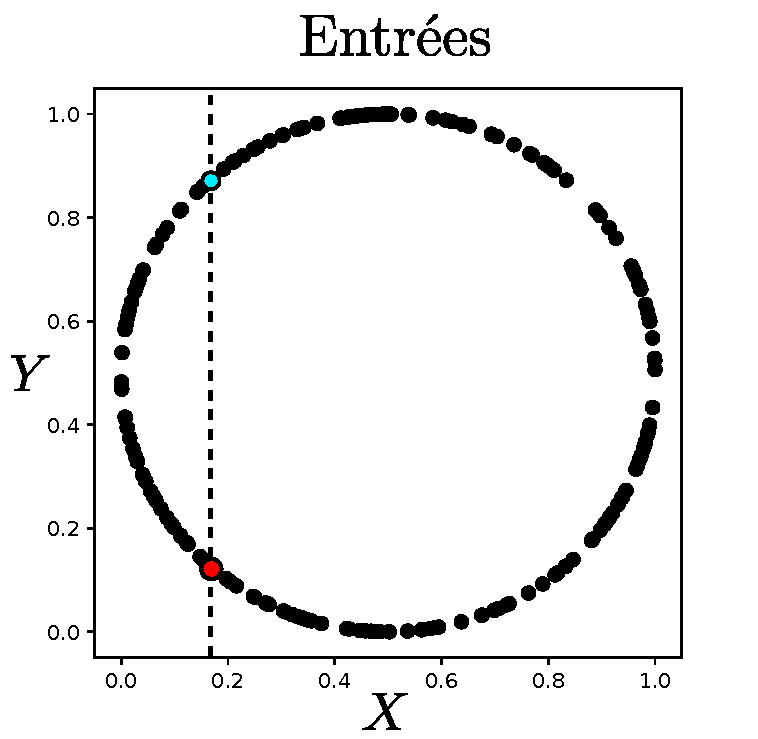
\includegraphics[width=0.8\textwidth]{2som_inp_noinformation}
\end{minipage}
\begin{minipage}{0.6\textwidth}
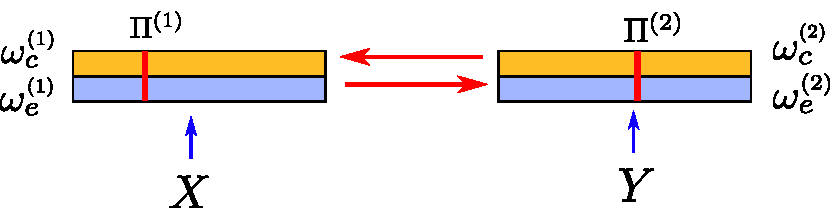
\includegraphics[width=\textwidth]{2som_archi}
\end{minipage}
\caption{A gauche, disposition des entrées dans l'exemple illustratif, sous forme de cercle. A droite, l'architecture de deux cartes en une dimension utilisée sur ces entrées dans ce chapitre pour illustrer les méthodes de représentation.\label{fig:exp}}
\end{figure}

\subsection{Représentations et indicateurs classiques des cartes de Kohonen}

Les cartes de Kohonen sont particulièrement associées à une facilité de représentation et de visualisation. Leur nombre réduit de prototypes et leur aspect topologique permet d'en tracer une représentation visuelle interprétable.
La manière la plus couramment utilisée de représenter une carte de Kohonen est de tracer les poids de ses prototypes, disposés dans le graphe (ligne ou grille) qu'est la carte. Deux exemples courants de représentation sont les suivants: 
\begin{itemize}
\item Le graphe qu'est la carte de Kohonen est représenté dans l'espace de ses positions (la grille d'indices $(i,j)$, ou une ligne indexée par $i$. Sur chaque noeud est tracé le poids correspondant. C'est le cas sur l'exemple de gauche en figure~\ref{fig:representation} dans lequel les poids des prototypes, qui sont des imagettes, sont affichés en chaque point de la grille. 
\item Lorsque les données traitées sont des points deux ou trois dimensions, les poids des prototypes peuvent être directement tracés dans l'espace $\mathbb{R}^2$ ou $\mathbb{R}^3$. Ces poids sont reliés en fonction des positions des n\oe{}uds dans la carte, montrant ainsi la déformation de la carte dans l'espace d'entrée, c'est le cas sur l'exemple de droite en figure~\ref{fig:representation} pour une grille en deux dimension.
\end{itemize}

Nous utiliserons des représentations adaptées au cas d'une architecture à plusieurs cartes à partir de ces deux modes de représentation. 
Cette adaptation dans le cas précis d'une architecture CxSOM est l'objet de cette section.

\begin{figure}
\begin{minipage}{0.5\textwidth}
\centering
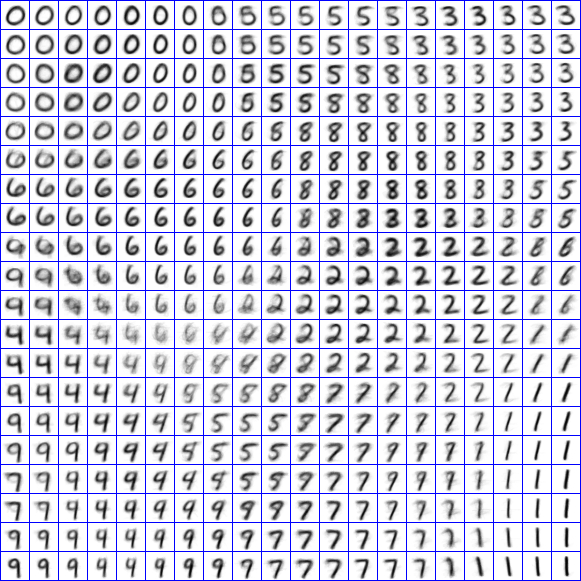
\includegraphics[width=0.5\textwidth]{digits.jpg}
\end{minipage}
\begin{minipage}{0.5\textwidth}
\centering
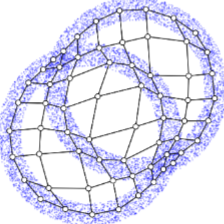
\includegraphics[width=0.5\textwidth]{points.png}
\end{minipage}
\caption{Représentations possible des poids d'une carte de Kohonen classiques, dans le cas d'entrées sous forme d'imagettes ou de points en deux dimensions.\label{fig:representation}}
\end{figure}

\subsection{Limites des représentations classiques dans le cas d'une architecture CxSOM}

Utilisons d'abord les représentations classiques mentionnées ci-dessus pour tracer les poids de chacun des cartes d'une architecture CxSOM à la fin de l'apprentissage.
La fin de l'apprentissage est définie comme le moment où les poids ont convergé vers une organisation restant stable au cours des itérations $t$.
La figure~\ref{fig:weights} présente le tracé des poids des deux cartes de l'exemple.
La courbe orange correspond aux poids externes des cartes, se dépliant sur chaque coordonnée $\inpx\m{1} = x$ et $\inpx\m{2} = y$ des points du cercle, appartenant chacune à $[0,1]$.
Ce tracé permet d'observer que les poids externes couvrent l'intervalle $[0,1]$, et sont organisés de façon monotone: ce comportement est celui qu'on attend dans une carte de Kohonen classique. Les poids contextuels, en bleu, ne présentent pas cette organisation monotone. Ils présentent toutefois une continuité: deux prototypes proches ont des poids proches. Le tracé des deux couches de poids nous informe donc sur le caractère continu de l'organisation de chacune de couches de poids. 

Notons que nous ne pouvons pas en tirer plus de conclusion: la représentation des poids de la figure~\ref{fig:weights} ne différencie pas les n\oe{}uds qui seront effectivement BMUs, des n\oe{}uds dits \emph{morts}.
Ces n\oe{}uds morts ont bien un poids, mais ne seront jamais BMUs.
Dans une carte de Kohonen classique, ces n\oe{}uds correspondent à des transitions, liant deux zones denses de l'espace d'entrée séparées par une zone sans points.
Par ailleurs, cette représentation concerne une seule carte. Nous ne pourrons pas tirer de conclusion sur l'influence des connexions entre cartes à partir de cette seule représentation.

Au regard des insuffisances des représentations classiques, que nous avons révélées sur un cas très simple de deux cartes mono-dimensionnelles, nous constatons qu'il est nécessaire de trouver un moyen de représenter l'architecture comme un tout. Nous devons ainsi définir des représentations qui montrent comment l'architecture de cartes est capable d'apprendre les relations entre les entrées multimodales.

\begin{figure}
\centering
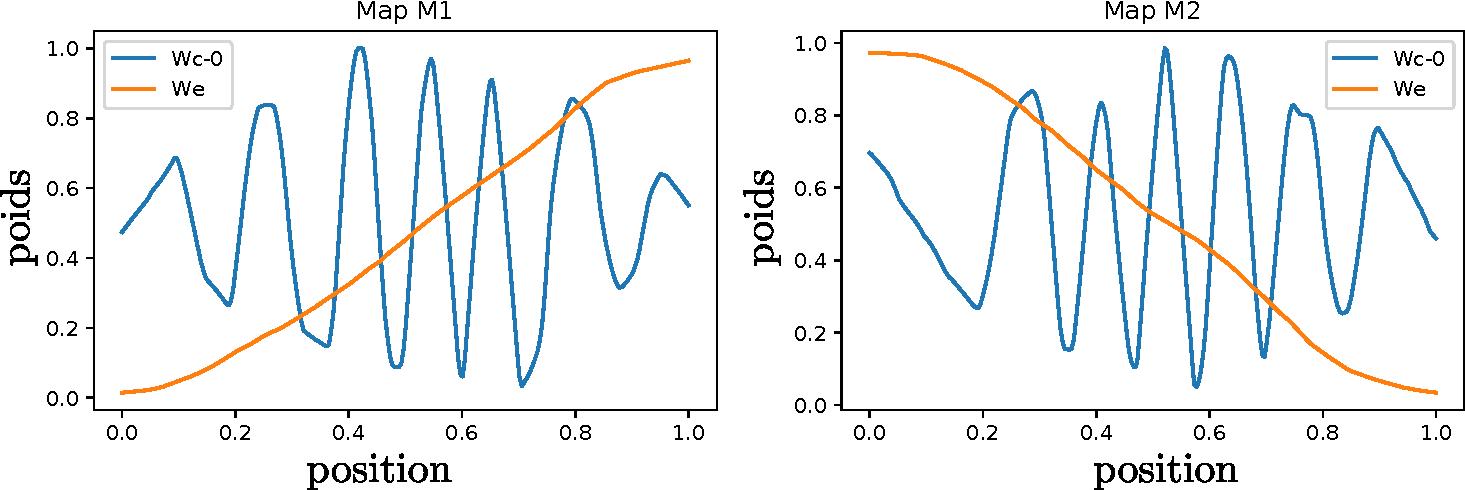
\includegraphics[width=0.9\textwidth]{weights_cercle1.pdf}

\caption{Représentation des valeurs des poids d'une carte au sein de CxSOM après apprentissage en fonction de leur position dans la carte. La seule représentation de ces poids ne suffit pas à savoir comment la carte se comporte.\label{fig:weights}}
\end{figure}

\subsection{Problématique}

Suite aux limites montrées par les méthodes de représentation classiques utilisées dans le domaine des SOMs, ce chapitre propose plusieurs façons de représenter une carte au sein d'une architecture.
Nous présenterons en premier lieu le formalisme décrivant les cartes et leurs entrées multimodales associées ainsi que la méthode expérimentale que nous utiliserons pour toutes les expériences présentées dans cette thèse. A partir de ce formalisme, nous proposerons plusieurs représentations permettant de comprendre et représenter ce que calcule une architecture CxSOM sur les données d'entrées. Ces représentations seront illustrées sur un exemple minimal de deux cartes pour faciliter la compréhension. Nous utiliserons ces méthodes dans les chapitres suivants pour analyser le comportement des cartes.

\section{Formalisation statistique des entrées et sorties des cartes}

Nous introduisons dans cette section un formalisme traitant les éléments des cartes et les entrées en tant que variables aléatoires. 
Ce formalisme possède à la fois l'avantage de clarifier les représentations et de permettre le développement d'indicateurs statistiques sur l'apprentissage effectué par les cartes.

\subsection{Formalisation des entrées}

Plaçons nous dans le cas général d'une architecture de $N$ cartes pour formaliser davantage.
Nous considérons des entrées multimodales tirées d'un ensemble d'espaces d'entrée $\mathcal{D}\m{1},\cdots,\mathcal{D}\m{n}$. Chaque espace $\mathcal{D}\m{i}$ est une modalité.
Les observations multimodales que l'on cherche à apprendre par l'architecture de cartes sont notées $(\inpx\m{i} \in \mathcal{D}\m{i}, i = 1 \cdots N)$.
Nous choisissons de modéliser ces entrées $\inpx\m{i}$ comme des \emph{variables aléatoires}.
Chaque variable aléatoire possède une distribution $p\m{i}$ sur $\mathcal{D}\m{i}$.
Nous notons $\mathbf{\inpx} = (\inpx\m{1}, \cdots, \inpx\m{n})$ la variable aléatoire jointe.
Cette variable appartient à l'espace $\mathcal{D}\m{1} \times \cdots \times \mathcal{D}\m{n}$.
A chaque pas de temps, un vecteur $\mathbf{\inpx} = (\inpx\m{1}_t, \cdots , \inpx\m{n}_t)$ est présenté à l'architecture: il s'agit d'une réalisation de la variable jointe $\mathbf{\inpx}$. 

En pratique, ces variables sont des observations, issues par exemple de capteurs d'un robot. Ces observations sont issues d'un environnement général et sont donc liées par des relations au sein de ce modèle d'environnement: les variables $\inpx\m{i}$ ne sont pas des variables indépendantes.
Nous introduisons la notion de \emph{modèle d'entrées} se rapportant à cette dépendance entre variables.
Le modèle d'entrée fait référence au modèle d'environnement permettant de générer les entrées multimodales fournies en entrées. Dans l'exemple d'illustration, les modalités sont les abscisses $\inpx\m{1} = x$ et les ordonnées $\inpx\m{2} = y$; le modèle d'entrées correspond au cercle, modélisé par une équation.

Le but de l'apprentissage non-supervisé par des cartes de Kohonen classiques est d'apprendre une représentation discrète de l'espace d'entrée.
Avec CxSOM, nous chercherons à la fois à apprendre un représentation discrète des espaces d'entrée mais aussi à apprendre une représentation du modèle d'entrées.

Les tracés que nous développerons dans cette section ont pour but de mesurer comment ce modèle d'entrées est représenté par l'architecture. 

\subsection{Formalisation du modèle d'entrée par une variable cachée}

Nous cherchons à évaluer expérimentalement la capacité du modèle CxSOM à apprendre à partir d'un environnement multimodal. Dans ce cadre expérimental particulier, nous choisissons des modèles d'entrées dont les relations sont connues. 
Ces modèles peuvent être paramétrisés par une variable multidimensionnelle $U$. Les modalités sont alors définies comme des fonctions de cette variable:
$\inpx\m{i} = f\m{i}(U)$
$U$ est une nouvelle variable aléatoire représentant le modèle.

Pour que la variable $U$ conserve toute l'information sur le modèle d'entrées, la fonction $(f\m{1}, \cdots, f\m{n})$ : $(\inpx\m{1}, \cdots \inpx\m{n})\rightarrow U$ doit être une bijection. Toute valeur d'entrées jointes correspond à un seul $U$, toute valeur de $U$ renvoie à une seule valeur d'entrées jointes. 
La définition de $U$ peut aussi être considérée comme un cas particulier de réduction de dimension du modèle, dans lequel la variable $U$, de dimension plus faible que $\mathbf{X}$, réduit la dimension des entrées sans perte d'information.

Dans le cas d'exemple, $\mathbf{X} = (\inpx\m{1},\inpx\m{2})$ est un vecteur aléatoire prenant comme valeurs les coordonnées cartésiennes des points du cercle de centre $x_c,y_c = 0.5,0.5$ et de rayon $r = 0.5$.
En définissant une variable $U$ scalaire à valeurs dans $[0,1]$, ces variables aléatoires peuvent maintenant s'écrire, selon l'équation paramétrique du cercle:
\begin{equation}
 \begin{cases}
     \inpx\m{1}= x_c + r  \cos(2\pi U)\\
     \inpx\m{2} = y_c + r \sin(2 \pi U)
    \end{cases}\,.
\end{equation}

$U$ représente ici l'angle du point sur le cercle (à un facteur $2\Pi$ près).
Ce modèle n'étant pas fourni à l'architecture de cartes lors de l'apprentissage, il s'agit d'un modèle \emph{latent}.
Nous cherchons, par l'architecture de cartes, à apprendre les entrées et les relations entre entrées: nous cherchons donc à extraire une structure dans le modèle latent. La relation entre $U$ et $\mathbf{X}$ est bijective; de ce fait, étudier comment l'architecture de cartes a appris $U$ est équivalent à étudier comment l'architecture a appris le modèle d'entrées.

Cet exemple est scalaire mais la représentation sous forme de variable cachée est générale à n'importe quel dimension et nombre d'entrées. En effet, toute configuration d'entrée multimodale dépend d'un environnement global. La variable $U$ correspond alors aux paramètres de cet environnement. Néanmoins, dans le cas de variables non artificielles, cette variable d'environnement est inconnue.
Nous utiliserons donc la variable cachée $U$ uniquement dans les expériences sur données artificielles. Elle nous permettra d'étudier et de représenter comment les cartes apprennent le modèle d'entrées.

\begin{figure}
\centering
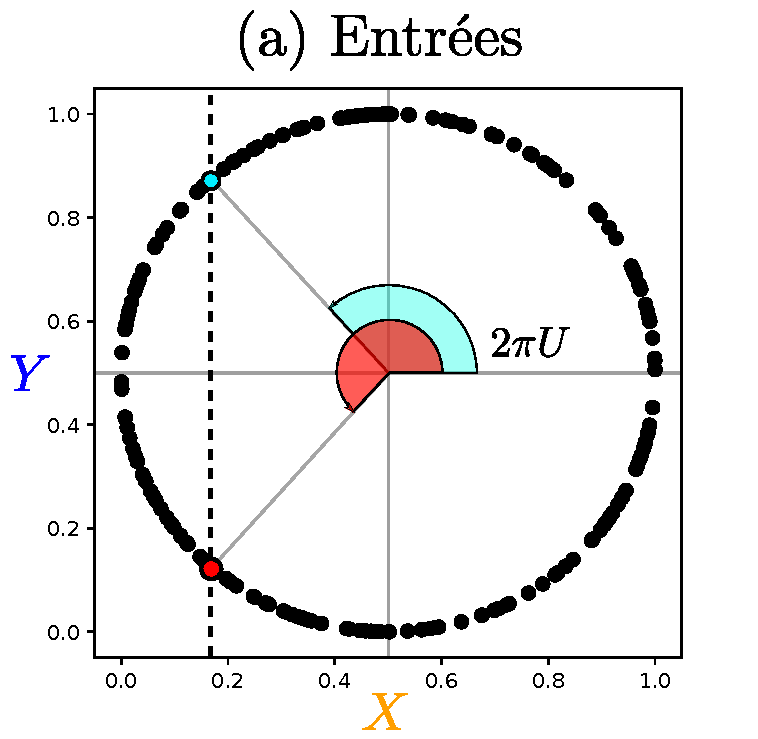
\includegraphics[width=0.4\textwidth]{2som_inp.pdf}
\caption{Représentation choisie pour le cercle. Le modèle auxquelles appartiennent les modalités $\inpx\m{1}$ et $\inpx\m{2}$ est représenté par la variable $U$. \label{fig:U}}
\end{figure}


\subsection{Démarche expérimentale}

Afin d'étudier le comportement de la carte à n'importe quel instant $t$ de l'apprentissage, nous effectuons une phase de \emph{test}, décrit en figure~\ref{fig:flowchart}.
Lors de cette phase de test, des entrées sont présentées à la carte, mais seul le processus de recherche de la best matching unit est réalisé, les poids des cartes ne sont pas mis à jour. Cet étape génère un ensemble de réponses de la carte aux entrées présentées.
Les entrées utilisées lors du test sont un échantillon de taille 1000 de la variable aléatoire $(\inpx\m{1}, \cdots, \inpx\m{n})$.
La distribution des entrées test est identique à la distribution des entrées d'apprentissage ayant servi au dépliement de la carte.

Nous formalisons non seulement les entrées mais aussi chaque élément de réponse des cartes d'une architecture comme une variable aléatoire.
Un élément de réponse d'une carte est une valeur régissant aux entrées lors d'une itération: positions du BMU, activité, poids du BMU.
Nous choisissons notamment de s'intéresser aux position des BMUs $\bmu\m{1}, \cdots, \bmu\m{n}$ et à leurs poids $\w\ext\m{1}(\bmu\m{1})$ et $\w\ext\m{2}(\bmu\m{2})$.
La valeur de ces éléments est indépendante entre deux itérations de test, car les poids ne sont pas mis à jour.
Grâce à cette indépendance entre itérations, les valeurs obtenues lors d'une phase de test forment un échantillon de la variable aléatoire jointe : 
$$(\underbrace{\inpx\m{1}, \cdots, \inpx\m{n}, U,}_{\text{Entrées}} \underbrace{\bmu\m{1}, \cdots, \bmu\m{n}, \w_e\m{1}(\bmu\m{1}), \cdots, \w_e\m{n}(\bmu\m{n})}_{\text{Eléments de réponse}})$$

Les composantes de cette variable jointe ne sont pas indépendantes. Maintenant que la démarche expérimentale est formalisées, les représentations présentées par la suite sont simplement des tracés de dépendances au sein d'un échantillon de test entre composantes de la variable jointe définie ci-dessus.

Les variables d'entrées sont à valeurs continues et $\bmu$ à valeurs discrètes, correspondant aux 500 n\oe{}uds d'une carte. Nous considérerons cependant $\bmu$ comme une variable continue plutôt qu'une grandeur discrète. En effet, l'ensemble des positions du BMU correspondent à une discrétisation de l'espace continu $[0,1]$, et sont ordonnées. Le déplacement par relaxation n'est pas limité aux positions discrètes des BMUs. Les variables aléatoires considérées sont bien à valeurs continues. Le formalisme par variable aléatoires permettra aussi d'utiliser des outils et métriques issus de la théorie de l'information pour qualifier l'organisation des cartes au sein de l'architecture, ce que nous ferons dans le chapitre~\ref{chap:indicateur}.

\begin{figure}
\centering
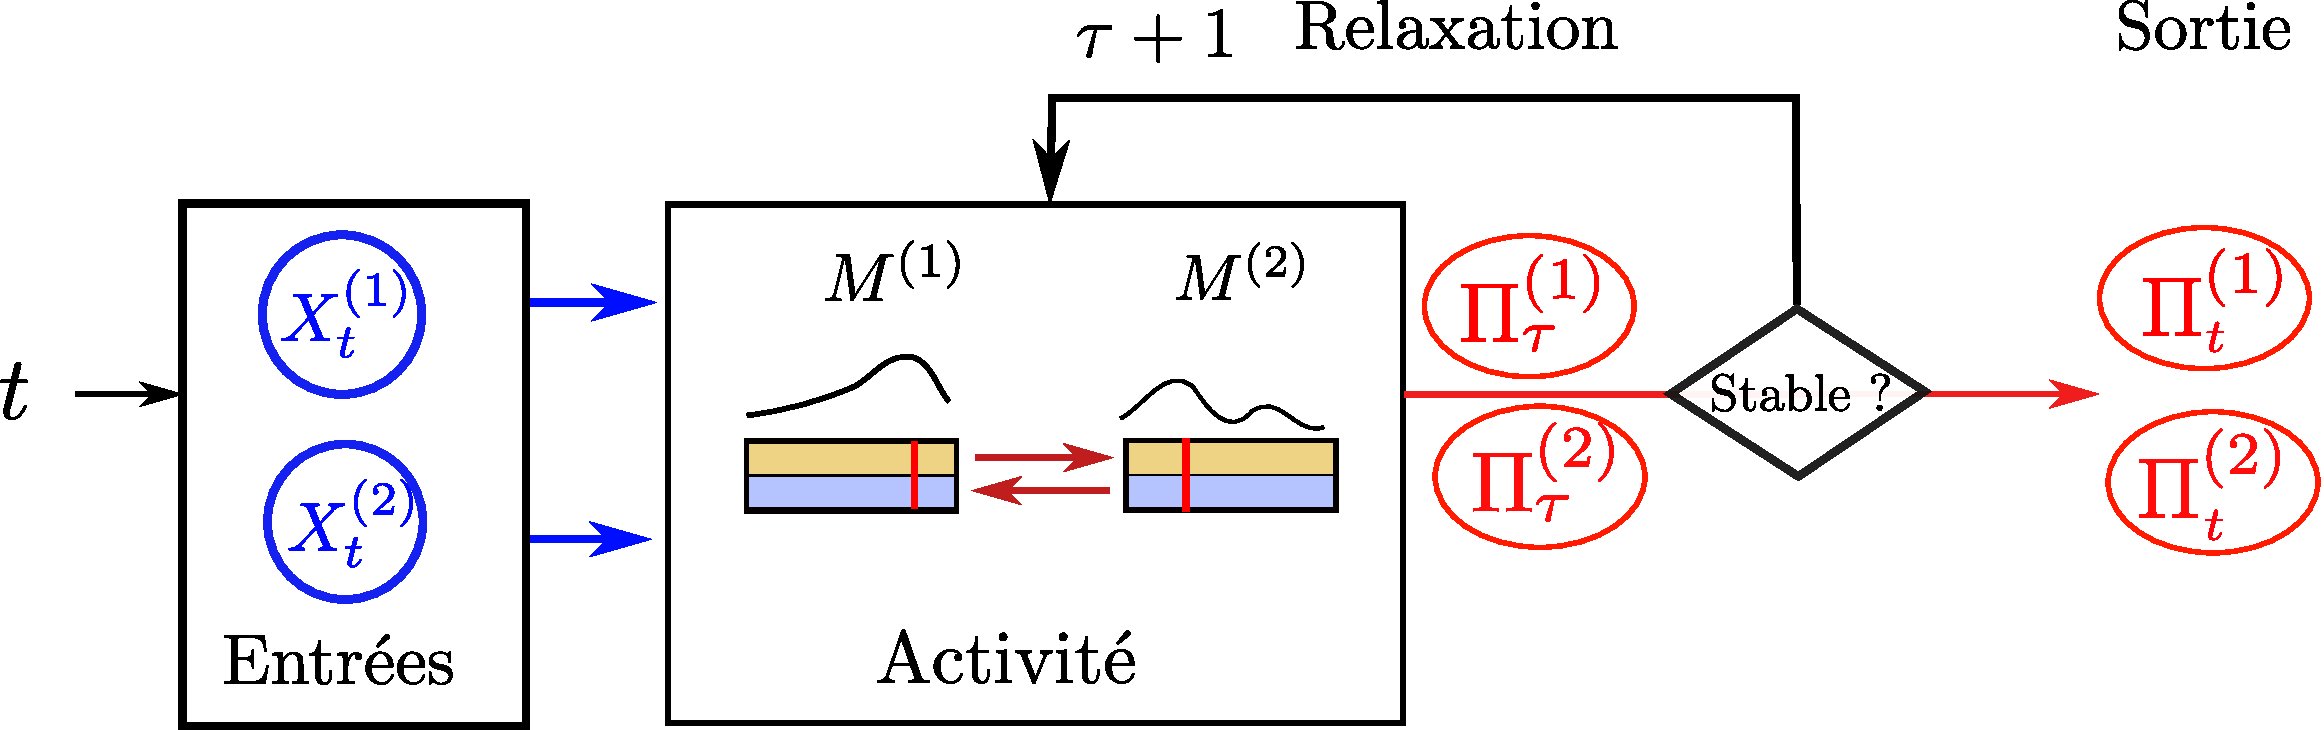
\includegraphics[width=0.85\textwidth]{tests_2maps.pdf}
\caption{Schéma décrivant une étape de test. Un test consiste à présenter successivement des réalisations de $\mathbf{X}$, notées $(\inpx\m{1}_t,\inpx\m{2}_t)$. Nous laissons le processus de relaxation stabiliser les BMUs. Quand la stabilité est atteinte, la valeur des positions de BMU $\bmu\m{1}_t$ et $\bmu\m{2}$ est obtenue. Un échantillon de test complet est ainsi obtenu en présentant un ensemble de réalisations de $\mathbf{X}$. Les poids ne sont pas mis à jour entre chaque itération, ce qui permet de considérer une phase de test comme un échantillonnage de la variable aléatoire $()\inpx\m{1},\inpx\m{2}, U, \bmu\m{1}, \bmu\m{2}$) }
\label{fig:flowchart}
\end{figure}

\section{Représentations graphiques}
A partir des échantillons de test, nous proposons dans cette section les représentations graphiques que nous utiliserons pour évaluer expérimentalement les architectures de cartes.
Ces représentations sont toute un tracé de dépendances entre des composantes de la variable $$(\inpx\m{1}, \cdots, \inpx\m{n}, U, \bmu\m{1}, \cdots, \bmu\m{n}, \w_e\m{1}(\bmu\m{1}), \cdots, \w_e\m{n}(\bmu\m{n}),U)$$ dont un échantillon est obtenu lors du test.
Nous proposons d'abord une représentation pour évaluer la qualité de quantification vectorielle effectuée par une carte de l'architecture. Nous présenterons ensuite des représentations nous permettant de comprendre comment le modèle d'entrées est appris par l'architecture CxSOM.

\subsection{Erreur de quantification d'une modalité dans chaque carte}

La première fonction d'une carte de Kohonen est de réaliser une tâche de quantification vectorielle sur son entrée externe. Au sein d'une architecture de cartes, nous nous attendons à ce que chaque carte extraie une représentation de la modalité qu'elle prend en entrée externe.
Afin de mesurer cette qualité de quantification vectorielle au sein d'une carte dans CxSOM, nous traçons le nuage de points correspondant au poids externe du BMU $\w_e(\bmu\m{i})$ en fonction de l'entrée externe présentée $\inpx\m{i}$. Une carte effectue une quantification vectorielle correcte si ce nuage de points est proche de la fonction identité.
Ces tracés sont réalisés en figure~\ref{fig:erreur} pour l'expérience exemple. Ces tracés s'approchent de l'identité: la quantification des entrées est correctement réalisée.
On pourrait mesurer une erreur quadratique moyenne pour déterminer numériquement cette erreur de quantification mais la représentation en nuage de points est, à défaut d'être quantitative, plus qualitative. En effet, ici, on observe que le nuage montre une structure "filamenteuse". Nous reviendrons sur ce point par la suite, nous contentant de souligner ici que la représentation graphique exprime une propriété que la simple mesure d'erreur n'aurait pas mise en évidence. 

Cette représentation nous informe ainsi sur la qualité de quantification dans une seule carte relativement à une seule modalité. Cette seule représentation est insuffisante à elle seule pour comprendre plus en détail le comportement d'une architecture de cartes: il nous faut également définir des méthodes de représentation permettant d'évaluer comment la structure globale du modèle d'entrées est apprise par l'architecture dans son ensemble.

\begin{figure}
    \centering
    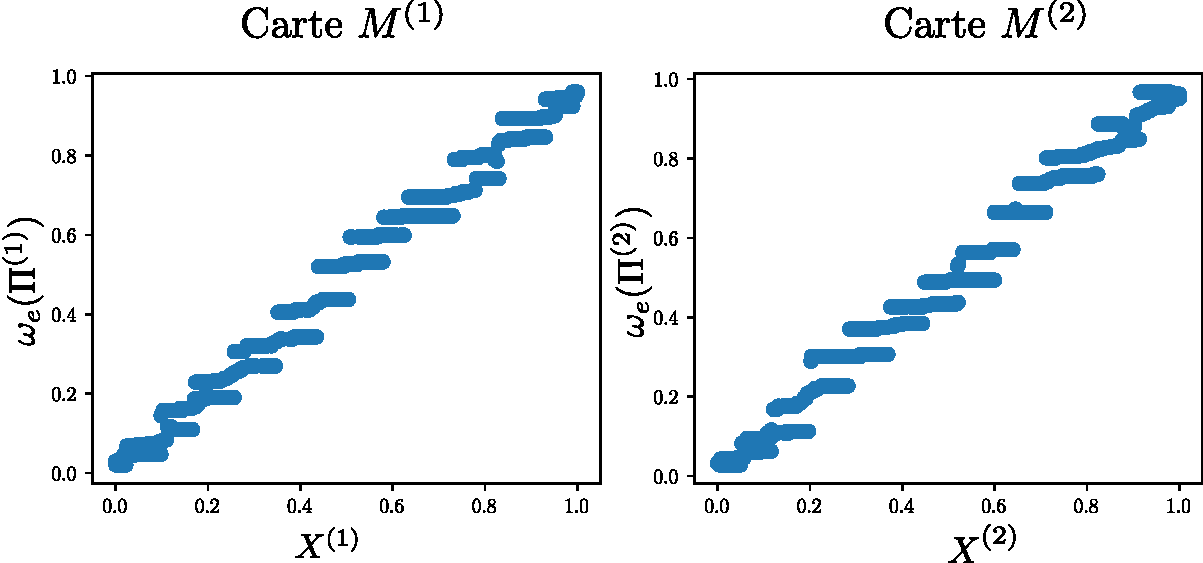
\includegraphics[width=0.7\textwidth]{w_x.pdf}
    \caption{Poids du BMU dans chaque carte en fonction de l'entrée présentée. On s'attend à des tracés proches de l'identité, montrant que le poids du BMU d'une carte est une bonne représentation de l'entrée. Sur ce graphique, on se rapproche effectivement de la fonction identité, cependant, une faible erreur est observée. On observe également un découpage des poids en bandes.\label{fig:erreur}}
\end{figure}


\subsection{Représentation cartographique des valeurs d'entrées préférentielles des BMUs}

En biologie, les aires du cortex cérébral sont cartographiées en faisant varier le motif d'entrée dans son espace, et en indiquant pour chaque neurone la valeur d'entrée préférentielle à laquelle il réagit. Cela donne alors une représentation cartographique où des valeurs de l'espace d'entrée sont tracées par rapport à la position sur le substrat neuronal du neurone qui y réagit.
Par exemple, une carte corticale est tracée pour l'aire visuelle primaire du cortex cérébrale, l'aire v1, en figure~\ref{fig:v1_repr}.

Un échantillon test donne un ensemble de valeurs de variable jointe $(\inpx\m{1}, \cdots, \inpx\m{n}, \bmu\m{1},\cdots, \bmu\m{n})$.
Dans la même idée que les cartes corticales, nous tracerons à partir de l'échantillon de test le nuage de points correspondant à la valeur de l'entrée $\inpx\m{i}$ d'une carte par rapport à la position du BMU $\bmu\m{i}$.
Cette représentation permet d'analyser la quantification des entrées par la carte. 
On s'attend à ce que les points soient proches de la courbe des poids externes de la carte $M\m{i}$.
Ce tracé fait également apparaître les zones dans lesquelles les neurones ne sont jamais best matching unit, les \emph{zones mortes}.
En plus des couples $(\bmu\m{i},\inpx\m{i})$, nous traçons également les entrées externes des autres cartes en fonction de $\bmu\m{i}$ : $(\bmu\m{i},\inpx\m{j})$.
Enfin, sur le même graphique, nous mettons ces valeurs d'entrées externes en relation avec les poids de la carte $M\m{i}$ en traçant les poids externes et contextuels de la carte $M\m{i}$ en fonction de leur position.
Une représentation cartographique fait ainsi apparaître les poids externes et contextuels d'une carte de l'architecture. A ces poids s'ajoutent plusieurs nuages de points correspondant aux valeurs d'une entrée $\inpx\m{j}$ en fonction du BMU de la carte $M\m{i}$, $\bmu\m{i}$.

En figure~\ref{fig:inputs}, nous avons ainsi tracé cette représentation cartographique pour l'exemple à deux cartes.
Nous y voyons deux nuages de points: $(\bmu\m{1},\inpx\m{1})$ et $(\bmu\m{1},\inpx\m{2})$ issus de l'expérience sur les deux cartes, ainsi que deux courbes: les poids externes et contexuels de la carte $M\m{1}$.
Deux valeurs issues de l'échantillon de test sont mise en évidence en couleur rouge et bleue sur chaque graphique. Un point de même couleur correspond à la même itération de test dans chaque graphique. Ces deux points partagent la même abscisse, donc l'entrée $\inpx\m{1}$ est la même pour ces deux échantillons. Par contre, leur ordonnée est différente: $M\m{2}$ reçoit donc une entrée $\inpx\m{2}$ différente entre de ces deux itérations.

Ce tracé nous permet d'abord d'observer que les points $(\bmu\m{1},\inpx\m{1})$ sont proches de la courbe de poids externe: le poids d'un BMU est proche de l'entrée qui a été présentée, le poids du BMU est donc une bonne approximation de cette entrée. Cela permet de conclure que la quantification vectorielle est bien réalisée dans cette carte sur les entrées externes, comme le montrait déjà la figure~\ref{fig:erreur}.

Tracer les échantillons de test permet ensuite d'observer la répartition des BMUs sur la carte. Les courbes de poids externes de la carte dans CxSOM (c) et de la carte indépendantes (b) sont indifférenciables; par contre, l'affichage de l'échantillon de test fait apparaître des zones mortes, sans BMUs. Nous observons ainsi que la carte au sein de CxSOM est découpée en plusieurs zones dans lesquelle les unités sont BMUs, séparées par des petites zones mortes. Ce tracé permet donc d'identifier un comportement nouveau dans une architecture de cartes, par rapport à une carte classique.

Les nuages de points $(\bmu\m{1},\inpx\m{1})$ et $(\bmu\m{1},\inpx\m{2})$ nous permettent d'observer quelles valeurs d'entrées sont codées dans les zones observées sur les positions des BMUs.
Nous observons notamment qu'une zone encode pour un intervalle de valeurs spécifique pour le couple $(\inpx\m{1},\inpx\m{2})$ et non seulement pour l'entrée externe de la carte, comme ce serait le cas dans une carte seule (b). Les points rouges et bleus illustrent ce comportement.
Ces échantillons correspondent à la même valeur d'entrée externe présentée à $M\m{1}$, mais $\inpx\m{2}$ est différent.
Dans la carte indépendante, le BMU sera identique pour ces deux valeurs.
Sur la figure (c), le point rouge et le point bleu ont leurs BMUs dans deux zones adjacentes, mais séparées, sur la carte.

La représentation des valeurs d'entrées $\inpx\m{j}$ selon la position du BMU $\bmu\m{i}$ permet ainsi d'identifier une répartition des BMUs sur une carte que nous ne pourrions pas observer en traçant simplement les poids.
Nous voyons notamment que la carte s'auto-organise en zones de BMUs, séparées par des zones mortes.
Les n\oe{}ds d'une zone réagissent à des valeurs spécifiques du couple d'entrées et non de seulement l'entrée externe.
Cette organisation en zone observée sur ce graphique traduit l'existence de deux échelles d'indices: une organisation primaire selon la valeur de l'entrée externe, et une organisation secondaire au sein des zones selon la valeur de l'entrée de l'autre carte.
Nous étudierons dans les chapitres suivants, grâce à cette représentation, si ce comportement se généralise pour différentes architectures et distributions d'entrées.

% Sur la figure (c), les BMUs appartenant à une même zone encodent les entrées $\inpx\m{1}$ ainsi que $\inpx\m{2}$ sur un intervalle particulier. Ce comportement diffère de celui de la carte simple (b). Dans cette carte, il n'y a pas de création de zones et un intervalle de position des BMUs encode deux intervalles distincts de valeurs concernant les entrées $\inpx\m{2}$.
% Les intervalles encodés par deux zones de BMUs adjacentes se recoupent: ce phénomène est illustré par le fait que les points rouges et bleus, ayant la même valeur de $\inpx\m{1}$, sont envoyés dans deux zones différentes.

% Ces valeurs peuvent être mises en relation avec celles de l'entrée $\inpx\m{2}$, également disposées selon $\bmu\m{1}$. Nous pouvons alors observer que deux zones adjacentes de la carte encodent des entrées proches selon $\inpx\m{1}$, mais très différentes pour $\inpx\m{2}$. Cela explique la séparation du point rouge et du point bleu dans deux zones.

\begin{figure}
    \centering
    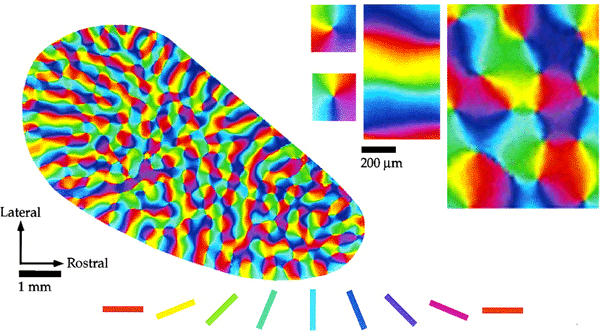
\includegraphics[width=0.7\textwidth]{v1.jpg}
    \caption{Carte corticale de l'aire cérébrale visuelle V1. Pour tracer cette représentation, un ensemble de traits de différentes orientation sont présentés en stimuli visuels au sujet, indiqués en bas de l'image. Le neurone réagissant à une entrée d'orientation particulière est coloré sur la carte de la couleur correspondante à l'entrée. Cette méthode permet de tracer des \emph{cartes corticales} d'une aire cérébrale \cite{Bosking1997OrientationSA}. \label{fig:v1_repr}}
\end{figure}

\begin{figure}
\begin{minipage}{0.27\textwidth}
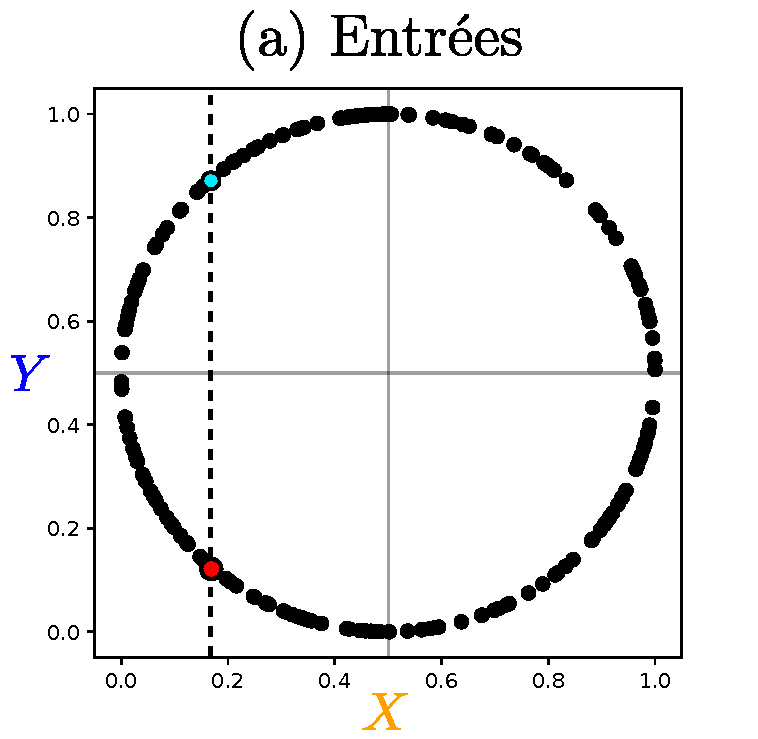
\includegraphics[width=\textwidth]{2som_inp_noU.pdf}
\end{minipage}
\begin{minipage}{0.34\textwidth}
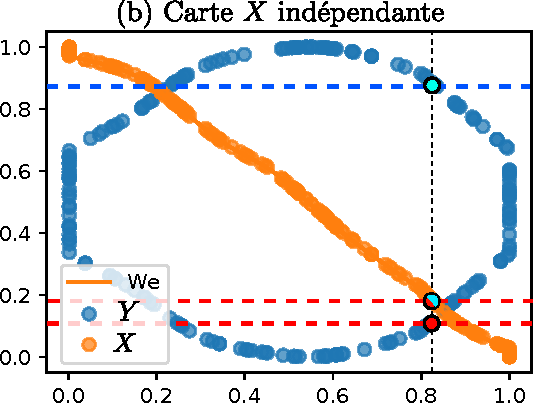
\includegraphics[width=\textwidth]{weights_2som_unco.pdf}
\end{minipage}
\begin{minipage}{0.38\textwidth}
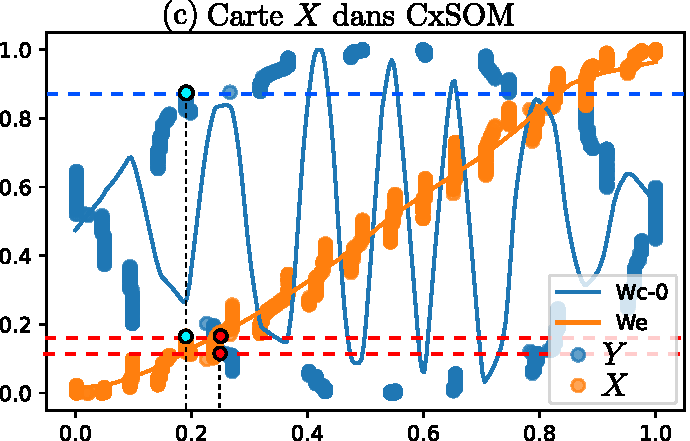
\includegraphics[width=\textwidth]{weights_2som.pdf}
\end{minipage}

\caption{Représentation des entrées $\inpx\m{1},\inpx\m{2}$ d'une architecture de deux cartes relativement au BMU de la carte $M\m{1}$ après apprentissage. Ces tracés mettent en valeur l'organisation des cartes, différentes dans le cas ou les cartes apprennent indépendemment leurs entrées~(b) ou sont connectées~(c). Les entrées correspondantes sont en figure~(a). Les points bleu et rouge reportés sur les tracés correspondent au même échantillon de test.\label{fig:inputs}}
\end{figure}

\subsection{Représentation de la variable cachée selon les positions des BMUs}

Nous avons vu lors de la représentation cartographique des entrées que chacune des cartes choisit son BMU  en fonction non seulement de son entrée externe, mais aussi de l'entrée de l'autre carte. Chaque carte s'organise donc en fonction du \emph{modèle d'entrée}, donc en fonction de $U$.
Afin de mettre en valeur ce comportement, nous tracerons les nuages de points représentant $U$ en fonction de la position $\bmu\m{i}$ du BMU d'une carte pour afficher comment la position du BMU traduit la relation entre les entrées.

En figure~\ref{fig:piu}, nous traçons $U$ en fonction de $\bmu\m{1}$ et $U$ en fonction de $\bmu\m{2}$.
Ce tracé montre $U$ comme une fonction de la position du BMU dans chaque carte, contrairement au cas ou les cartes ne sont pas connectées pour lequel deux valeurs de $U$ correspondent à un même BMU. Cela traduit bien le fait que chaque carte a appris une représentation du modèle d'entrée et non seulement de son entrée externe.
L'organisation de la carte dans CxSOM montre donc chaque position $\bmu$ codant pour une seule valeur de $U$, c'est à dire une seule position d'échantillon sur le cercle.
La représentation de $U$ selon la position du BMU d'une carte $\bmu\m{i}$ permet de représenter comment la carte $i$ a appris l'ensemble d'entrées $(\inpx\m{1},\inpx\m{2})$ et non seulement son entrée externe. Déterminer si l'architecture a appris le modèle d'entrées revient alors à vérifier si $U$ est une fonction de $\bmu$ dans chacune des cartes de l'architecture.

Cette représentation fait appararaître $U$ comme une fonction de $\bmu$ dans chaque carte. Ce comportement traduit le fait que les cartes s'organisent en fonction de tout le modèle d'entrée, non seulement de leur entrée externe. Il s'agit là d'un comportement que nous pouvons qualifier de comportement de base pour CxSOM. 

\begin{figure}
\centering
\includegraphics[width = 0.7\textwidth]{xu_yu_both.pdf}
\caption{Valeur de $U$ en fonction des valeurs du BMU $\bmu\m{i}$ dans chacune des cartes dans l'exemple d'illustration. Sur la première ligne, nous traçons la réponse de chaque carte à son entrée dans le cas ou les deux cartes ne sont pas connectées. Sur la deuxième ligne, nous traçons la réponse de chaque carte lorsqu'elles ont appris de façon jointe au sein de CxSOM.
$U$ apparaît alors comme une fonction de la position du BMU $\bmu\m{i}$ dans chaque carte, contrairement au cas ou les cartes apprendraient indépendamment sur les mêmes entrées. Cette relation fonctionnelle est symbolisée par les pointillés sur les tracés du bas. Les mêmes échantillons rouge et bleu mis en évidence en figure~\ref{fig:inputs} sont reportés sur les tracés.}
\label{fig:piu}
\end{figure}


\subsection{Dépliement d'une carte dans l'espace d'entrée multimodal}

Une représentation classique utilisée pour représenter une carte de Kohonen est de tracer les poids du graphe qu'est la carte dans l'espace de ses entrées, telle qu'en figure de droite en~\ref{fig:representation}. Dans CxSOM, chaque carte prend en entrée une seule des modalités. Par contre, grâce à l'échantillon de test, il est possible de représenter comment la carte se déplie dans l'espace de toutes les modalités.

Nous définissons alors une façon de représenter le dépliement d'une seule carte de CxSOM dans l'espace global des entrées. Dans l'exemple, il s'agit de représenter le dépliement de $M\m{1}$ dans l'espace des entrées $\inpx\m{1},\inpx\m{2}$.
Au lieu de s'appuyer sur les poids des cartes comme en~\ref{fig:representation}, nous utilisons les valeurs de l'échantillon de test. Nous traçons le nuage de poids correspondant au poids des BMUs: $\w_e\m{1}(\bmu\m{1},\w_e\m{2}(\bmu\m{2})$, puis relions ces points selon l'ordre de leurs positions dans la carte $M\m{1}$ ou $M\m{2}$. Ainsi, nous obtenons une représentation des cartes $M\m{1}$ ou $M\m{2}$ dépliées dans l'espace global des entrées. 
Notons que les unités mortes ne peuvent pas être représentées sur la carte. Nous ne représentons que les morceaux de cartes étant effectivement BMUs. 
Cette représentation est tracée en ~\ref{fig:distortion} pour l'exemple à deux cartes.


La carte représentant les poids externes des BMUs, on s'attend à ce que la forme du nuage de points corresponde à la structure des entrées.
Les tracés mettent en lumière les propriétés observées lors de la représentation cartographique des entrées, à savoir l'apparition de zones dans chaque carte. Les poids suivent la structure circulaire des entrées en découpant l'espace en zones. Les parties du cercle effectivement représentées par les poids sont réduites: le cercle est comme discrétisé en petits morceaux.
Dans l'exemple, on remarque la façon dont est parcouru l'espace dans chaque carte: en fonction de $x$ dans la carte $M\m{1}$, et en fonction de $y$ dans la carte $M\m{2}$. 
Cette représentation offre la possibilité  de visualiser comment une carte se déplie dans l'espace d'autres modalités.

\begin{figure}
    \begin{minipage}{0.49\textwidth}
    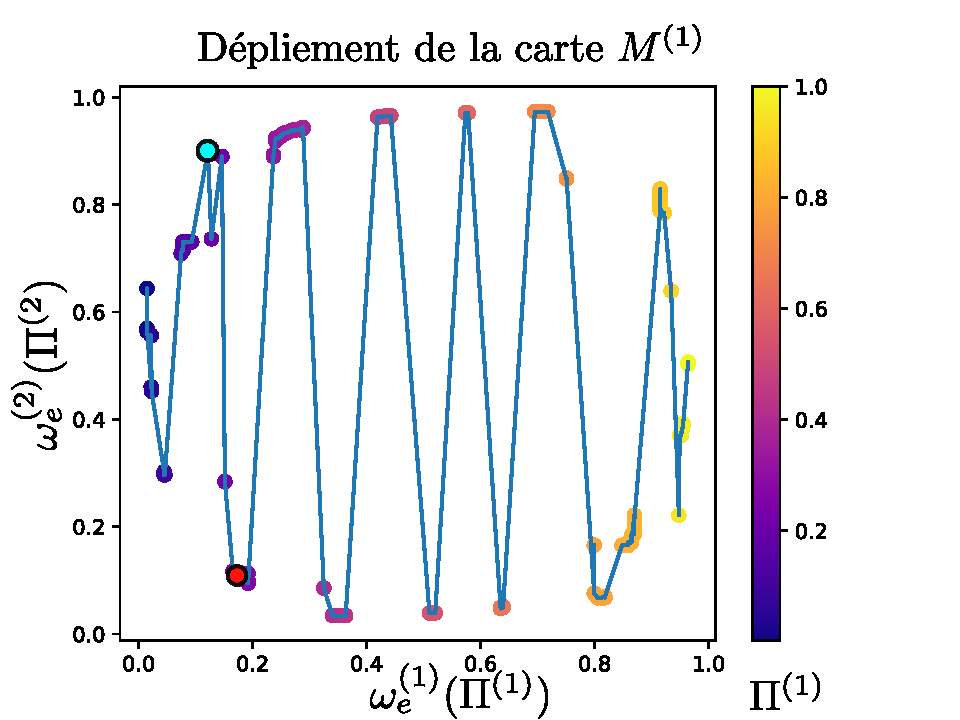
\includegraphics[width=\textwidth]{disto_cercle_M1.pdf}
    \end{minipage}
    \begin{minipage}{0.49\textwidth}
    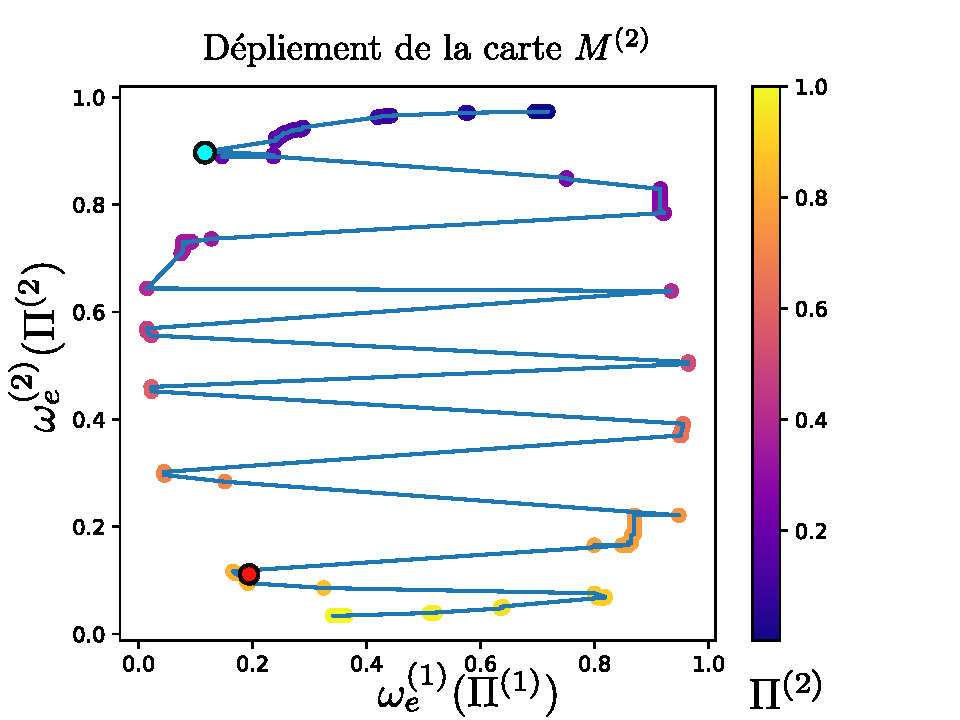
\includegraphics[width=\textwidth]{disto_cercle_M2.pdf}
    \end{minipage}
    \caption{Dépliement des cartes $M\m{1}$ et $M\m{2}$, reliés dans l'ordre de leurs positions selon $M\m{1}$ figure de gauche et $M\m{2}$ figure de droite. Le dépliement de chacune des cartes est alors représenté dans l'espace complet des entrées \label{fig:distortion}. L'indice du BMU est signalé par la carte de couleurs, différenciant ainsi les extrémités en 0 et 1 des cartes.}
    \end{figure}


\section{Conclusion}

Afin d'extraire des comportements d'une architecture de cartes, nous modélisons les éléments des cartes comme des variables aléatoires et l'étape de test comme l'échantillonnage d'une variable jointe. Nous introduisons notamment, dans le cas des exemples artificiels, une variable cachée $U$ non présentée comme entrée à la carte, portant toute l'information sur le modèle d'entrées.
La représentation par échantillonnage et variable aléatoire permet de mieux comprendre les mécanismes des cartes, ceux ci ne reposant plus directement sur les courbes de poids.

Nous utiliserons donc quatre représentations des cartes dans la suite de cette thèse, toutes définies à partir d'un échantillon de test.
Le tracé du poids du BMU en fonction de l'entrée externe permet d'évaluer comment chaque carte extrait une représentation de son espace d'entrée.
La représentation cartographique des entrées selon le BMU de chaque carte fait apparaître des zones mortes dans les cartes CxSOM et affiche les valeurs préférentielles d'entrées selon leur BMU. Cette représentation met en lumière un comportement émergeant de l'exemple à deux cartes: de façon auto-organisée, chaque carte définit des zones de BMUs correspondant à intervalle de valeurs $(\inpx\m{1},\inpx\m{2})$, et non seulement $\inpx\m{1}$. Cette représentation fait également apparaître une notion d'organisation selon un indice primaire sur les poids externes, et secondaire grâce aux poids contextuels. Nous étudierons plus extensivement ce comportement dans la partie suivante grâce à cette représentations.
Afin d'évaluer la façon dont un BMU traduit le modèle d'entrée, nous traçons la variable cachée $U$ en fonction du BMU d'une carte $\bmu\m{i}$.
L'apprentissage du modèle d'entrée se traduit alors par l'observation d'une \emph{relation fonctionnelle} entre $U$ et $\bmu$ dans chaque carte.
Enfin, nous proposons une représentation du dépliement de chaque carte dans l'espace de toutes les entrées en traçant les poids des BMUs de chaque carte, ordonnés selon les BMUs d'une des cartes. Cette représentation apporte une vision globale de la façon dont une carte encode le modèle d'entrées.
Ces représentations permettront d'étudier plus en détail les comportements observés dans l'exemple illustratif. Cette étude sera traitée au chapitre~\ref{chap:analyse}.

Même avec des représentations adaptées, l'analyse d'architectures comportant de nombreuses cartes ne peut pas simplement s'effectuer à l'aide de graphiques, qui deviendraient trop complexes. La comparaison d'un grand nombre d'expériences est aussi difficilement réalisable graphiquement.
Cette difficulté de représentation et le besoin de comparer des expériences soulève la nécessité de définir une valeurs indicatrice du fonctionnement de la carte, que nous proposerons dans le chapitre suivant.


\comment{Correlation ration : mesure de dépendance fonctionnelle
Débruitage de l'IM : répétition de l'expérience et moyenne ?}
\draft{Le ration de corrélation traduit mieux que le coefficient d'incertitude la dépendance fonctionnelle entre le modèle et le BMU. Cependant, à l'inverse de l'information mutuelle, une relation non fonctionnelle mais précise (telle que l'exemple du cercle de la figure~\ref{fig:exemple-limite}) entre les variables aura un score très faible. Ce n'est pas non plus voulu. 

Il semble que l'information mutuelle reste le moyen le plus prometteur et le plus général de mesurer la relation entre les éléments des cartes. Dans le cas une dimension, on observe qu'on veut tendre vers U fonction du BMU; on connait mal le comportement recherché en dimension plus grande (cartes 2D, entrées de grande dimension). L'information mutuelle laisse donc l'opportunité à plus d'états d'organisation des cartes de l'architecture d'avoir un bon score. La meilleure perspective serait donc de pouvoir calculer le coefficient d'incertitude sur des échantillons provenant de données non bruitées, ou de pouvoir séparer le bruit des données lors du calcul du coefficient.
Dans cette optique, l'estimateur par histogrammes permet de réduire l'effet du bruit, en choisissant correctement les tailles de boîtes. L'utilisation histo versus Kraskov reste donc à discuter.
Dans le cas ou le modèle d'entrée est connu, calculer les réponses des cartes sur des jeux de données non bruitées générées artificiellement, après apprentissage sur un jeu de données réelles et bruitée, est une solution. Si le modèle n'est pas connu, des méthodes statistique de réduction de bruit peuvent être imaginées.} 

\draft{
\section{Prédiction d'entrée}

Au sein d'une architecture de cartes, il est possible de ne pas présenter à une ou plusieurs cartes de l'architecture leur entrée externe $\inpx\m{i}$. Dans ce cas, une best matching unit peut quand même être calculée par leurs entrées contextuelles. Le poids de cette best matching unit peut alors être vu comme une prédiction de l'entrée manquante. Cette capacité de prédiction peut être à la fois vue comme une application possible de l'architecture, mais aussi comme une façon de représenter \emph{ce que les autre cartes connaissent d'une autre}. Tracer les prédictions d'une carte est donc un indicateur de la façon dont une architecture a appris des relations. 


\comment{
2 parties dans estimation/perspectives : 
d'une part, questionnement sur l'estimation des données bruitées par exemple - pas besoin de proposer des solutions si elles ne sont pas testées ? 
Et parler de l'estimation en grande dimension : ce n'est pas forcément le pb ici. Donc pas la peine...
}
}

\documentclass[../main]{subfiles}
\ifSubfilesClassLoaded{
    \addbibresource{../Biblio/biblio.bib}
    \dominitoc
    \tableofcontentsfile
    \pagenumbering{arabic}
    \setcounter{page}{1}
    \setcounter{chapter}{5}
}{}
\begin{document}
\chapter{Indicateurs numériques de l'apprentissage du modèle d'entrées \label{chap:indicateur}}
\graphicspath{{05-Indicateur/figures},{./figures/}}
\minitoc

\section{Introduction}

Dans les chapitres~\ref{chap:repr} et \ref{chap:analyse}, nous avons identifié des mécanismes caractérisant l'apprentissage d'un modèle d'entrées au sein de l'architecture de cartes en s'appuyant sur les représentations graphiques des poids et des BMU.
Nous avons souligné l'importance de développer des indicateurs numériques pour mesurer cet apprentissage, afin de faciliter la comparaison entre différentes expériences et l'optimisation des paramètres d'apprentissage.

Nous avons représenté les modèles d'entrées à apprendre grâce une variable latente $U$, qui traduit les paramètres libres du modèle d'entrées.
Les représentations graphiques nous ont permis de constater que l'apprentissage du modèle d'entrées se caractérise par une relation fonctionnelle entre $U$ et la position du BMU $\bmu$ dans chaque carte.
Dans ce chapitre, nous étudions deux méthodes mesurant la qualité de cette relation fonctionnelle~: le coefficient d'incertitude, qui est une version normalisée de l'information mutuelle, et le ratio de corrélation.
Ces méthodes s'appuient sur la représentation des entrées et réponses des cartes vues comme des variables aléatoires.
Nous spécifierons ce que nous attendons de cette relation fonctionnelle dans le cadre de l'architecture, et comparerons la capacité de ces deux méthodes à traduire cette relation afin d'identifier leurs limites et de déterminer l'indicateur numérique le plus adapté.

Nous avons également soulevé que pour des architectures de grande taille ou lorsque $U$ est de grande dimension, $U$ pourrait ne pas être une fonction de $\bmu$ dans chaque carte. Une représentation distribuée de $U$ entre les cartes, tout en présentant une certaine redondance en terme d'information, pourrait être préférable.
La dernière partie de chapitre porte ainsi sur des possibilités d'utilisation de l'information mutuelle comme indicateur de l'apprentissage du modèle dans une structure de cartes.

\section{\'Eléments de théorie de l'information}

Les indicateurs que nous examinons sont issus de la théorie de l'information. Nous proposons ici d'introduire les principales notions utiles à la présentation des indicateurs et à leur interprétation.

\subsection{Entropie et information mutuelle}

Les notions d'entropie et les valeurs associées, telle que l'information mutuelle entre des variables aléatoires, sont des notions fondamentales de la théorie de l'information de Shannon \parencite{Shannon1948AMT}. Ces quantités sont calculées à partir de la distribution des variables aléatoires.
L'entropie de Shannon d'une variable aléatoire $X$ à valeurs dans un ensemble $\Omega_X$ discret, de distribution $P_X$, est notée $H(X)$ et définie par~: 
\begin{equation}\label{eq:H}
H(X) = - \sum_{x \in \Omega_X}{P_X(x)\textrm{log}(P_X(x))}
\end{equation}

L'entropie de Shannon concerne uniquement des variables discrètes.
Une autre version de l'entropie est définie pour des variables continues, l'entropie différentielle~:
\begin{equation}
    h(X) = - \int_{x \in \Omega_X}{p_X(x)\textrm{log}(p_X(x))dx}
\end{equation}
Avec $p_X$ la densité de probabilité de $X$.
Notons que l'entropie différentielle n'est pas la limite de l'entropie de Shannon calculée par discrétisation de $X$ en $N$ intervalles, $N \rightarrow \infty$. L'entropie différentielle peut prendre des valeurs négatives.

L'existence d'une relation quelconque entre deux variables aléatoires $X$ et $Y$ à valeurs dans $\Omega_X$ et $\Omega_Y$ se mesure par leur information mutuelle.

Elle est définie par : 
\begin{equation}\label{eq:MI}
 I(X,Y) = \sum_{x,y \in \Omega_X,\Omega_Y}{P_{XY}(x,y)\textrm{log}(\frac{P_{XY}(x,y)}{P_X(x)P_Y(y)})}
\end{equation}

Avec $P_{XY}$ la distribution de la variable aléatoire jointe $(X,Y)$.
Cette valeur mesure la quantité d'information moyenne partagée entre les distributions $X$ et $Y$~: en moyenne, quelle information sur la valeur de $Y$ donne une valeur de $X$ et inversement, quelle information sur la valeur de $X$ donne une valeur de $Y$.

L'information mutuelle possède notamment les propriétés suivantes~:
\begin{enumerate}
\item $I(X,Y) = 0 \Leftrightarrow \textrm{X et Y sont indépendantes}$. L'information mutuelle peut être vue comme une mesure de la distance entre la distribution jointe de $(X,Y)$, $P_{XY}(X,Y)$ et la distribution correspondant à l'indépendance des variables, $P_X(X)P_Y(Y)$.
\item\label{it:h} Elle s'exprime à partir de l'entropie de Shannon : $I(X,Y) = H(X) + H(Y) - H(X,Y) = H(X) - H(X|Y) = H(Y) - H(Y|X)$
\item Elle est symétrique : $I(X,Y) = I(Y,X)$
\item\label{it:eq} Pour toute fonction $f$, $I(X,Y) \geq I(X,f(Y))$. L'égalité est atteinte si et seulement si $f$ est bijective.
\end{enumerate}

L'information mutuelle se calcule également à partir des densités de probabilité pour des variables à valeur continues de densités de probabilité $p_X$ et $p_Y$~:
\begin{equation}
    I(X,Y) = \int_{x \in \Omega_X}\int_{y \in \Omega_Y }{p_{XY}(x,y)\textrm{log}(\frac{p_{XY}(x,y)}{p_X(x)p_Y(y)})dx \: dy}
\end{equation}

Contrairement à l'entropie, la valeur de l'information mutuelle pour des variables continues correspond bien à une limite des valeurs de l'information mutuelle discrète lorsque le nombre de catégories tend vers l'infini \parencite{Cover2005ElementsOI}.
Cependant, dans le cas continu, les propriétés \ref{it:h} et \ref{it:eq} ne sont pas vérifiées. 
En particulier, $I(X,X) \neq h(x)$ comme c'est le cas pour des variables discrètes. En effet, $h(X|X) = - \infty$.

\subsection{Méthodes d'estimation}\label{sec:estimation}
\begin{figure}
    \begin{minipage}{0.4\textwidth}
    \centering
    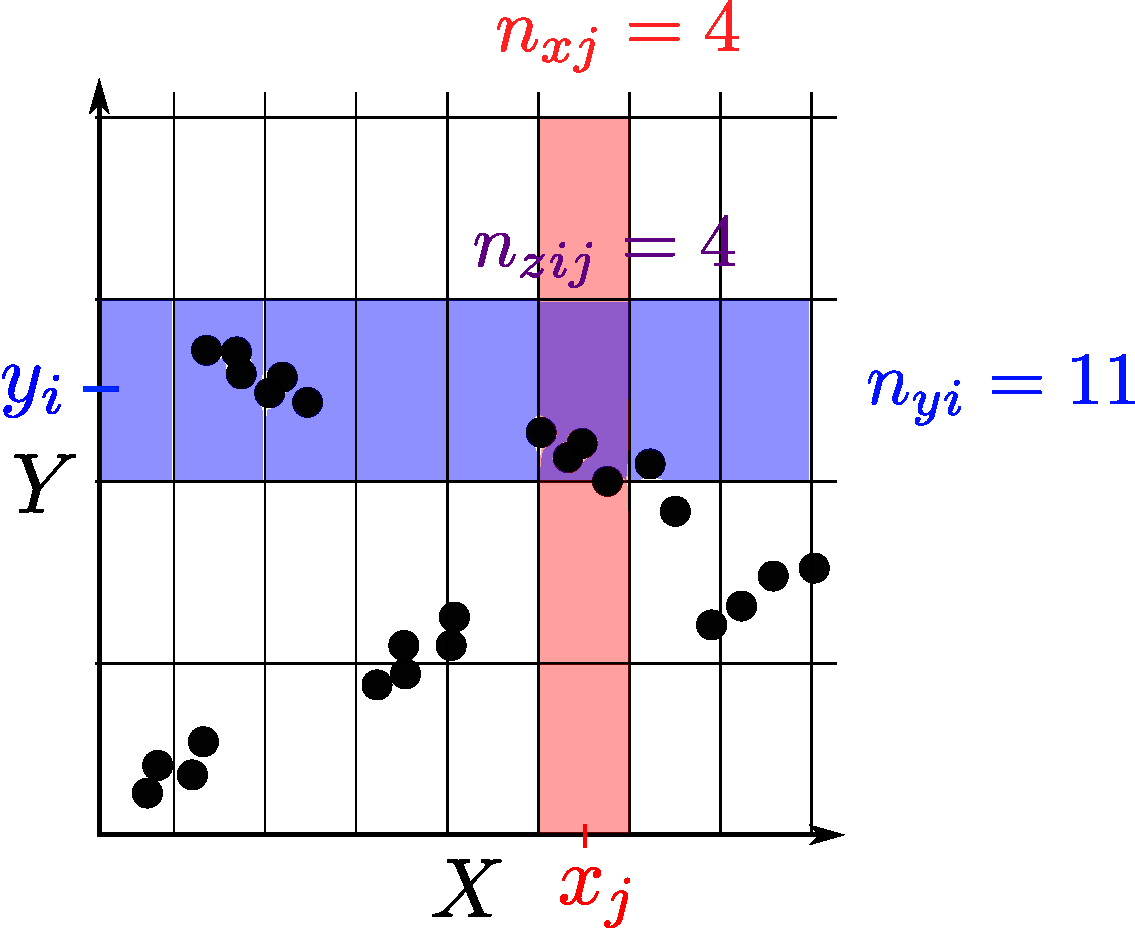
\includegraphics[width=\textwidth]{boxes}
    \caption{Méthode d'estimation par histogrammes des distributions des variables $X$ et $Y$. Les distributions sont estimées à partir de $n_{xj}$, $n_{yi}$ et $n_{zij}$, ce qui permet d'estimer l'information mutuelle et l'entropie de Shannon selon \ref{eq:MI} et \ref{eq:H}}
    \label{fig:binning}  
    \end{minipage}
    \hfill
    \begin{minipage}{0.55\textwidth}    
            \centering
            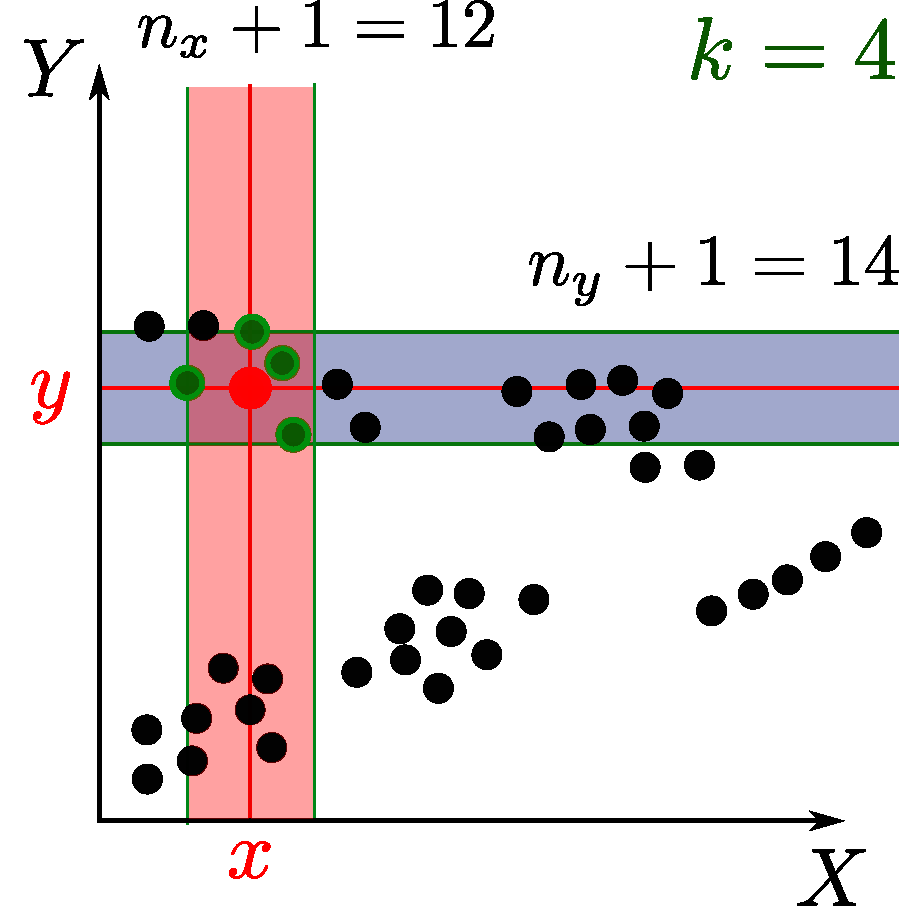
\includegraphics[width=0.55\textwidth]{kraskov.pdf}
            \caption{Méthode d'estimation d'information mutuelle par \emph{k-nearest neighbors}. Les plus proches voisins de chaque point (indiqués en vert pour le point marqué en rouge) déterminent une fenêtre selon chaque axe. Les valeurs de $n_x$ et $n_y$ permettent d'estimer directement l'information mutuelle (voir équation~\ref{eq:knn}).}
            \label{fig:kraskov}
    \end{minipage}
    \end{figure}

L'information mutuelle et l'entropie sont des grandeurs définies à partir de la distribution des variables aléatoires. Nous ne connaissons pas leur distribution et devons donc estimer ces quantités à partir des échantillons de données. 
Nous nous intéresserons en particulier à l'information mutuelle entre les variables $U$ et $\bmu$, qui sont des variables continues. Nous présentons deux méthodes classiques d'estimation de l'information mutuelle pour des variables continues.


Une première méthode d'estimation classique est la méthode des histogrammes (\emph{binning}).
Cette méthode s'appuie sur une estimation de la distribution des variables $X$, $Y$ et la distribution de la variable jointe $(X,Y)$ en discrétisant chacune des variables.
Cette méthode est représentée en figure~\ref{fig:binning}. Les variables $X$ et $Y$ sont discrétisées en \emph{bins} de centres $x_i$ et $y_j$ choisis.
La distribution de chaque variable est alors estimée par~: 
$$P(X = x_i) = \frac{n_{xi}}{N} $$ où $n_{xi}$ est le nombre d'échantillons de $X$ tombant dans le \emph{bin} de centre $x_i$ et $N$ le nombre de points. Le même procédé est réalisé pour $Y$ et $(X,Y)$. La précision de l'estimation peut être améliorée en choisissant des tailles de \emph{bins} variables~; nous utilisons ici la méthode simple avec des \emph{bins} de taille fixe.
% Pour des variables à valeurs dans $[0,1]$, les centres sont définis par $x_k = \frac{k}{M}+\frac{1}{2M}$, avec $M$ le nombre de \emph{bins}.
Après cette discrétisation, l'estimation de l'entropie et l'information mutuelle des variables est calculée selon les équations~\ref{eq:H} et \ref{eq:MI}.
La valeur de cet indicateur est très sensible à la résolution choisie pour le calcul des histogrammes, c'est-à-dire le nombre de \emph{bins}.
Par ailleurs, plus ce nombre de \emph{bins} augmente, plus le nombre de points disponibles pour l'estimation doit augmenter. C'est en particulier le cas lorsque la dimension des entrées augmente~:
le nombre d'échantillons disponibles pour l'estimation doit augmenter exponentiellement avec la dimension des variables. En effet, à cause de la faible densité des données, de nombreux \emph{bins} ne contiendront pas de points pour l'estimation alors qu'ils auraient dû en contenir d'après leur distribution théorique, ce qui fausse l'estimation.

Une deuxième méthode communément utilisée pour l'estimation de l'information mutuelle est l'estimateur par \emph{K-Nearest Neighbors} \parencite{2004kraskov}, présenté en figure~\ref{fig:kraskov}.
Cet estimateur ne passe pas par l'estimation de la densité de probabilité, contrairement aux histogrammes, mais estime directement l'information mutuelle.
Le découpage de l'espace se fait en recherchant, pour $N$ valeurs d'échantillons d'un couple $(X,Y)$, les $k$ plus proches voisins, ce qui détermine une fenêtre. Une information mutuelle locale est calculée dans cette zone de l'espace, suivant une formule permettant d'approximer les différences de logarithme par la fonction digamma $\psi$ : 
$$i_j(X,Y) = \psi(k) - \psi(n_{x_j} + 1) - \psi(n_{y_j} +1) + \psi(N)$$
Cette information mutuelle locale est ensuite moyennée sur l'ensemble des points (en notant $\langle \rangle$ l'opérateur de moyenne) ~: 
\begin{equation}\label{eq:knn}
    \hat{I}(X,Y) = \psi(k) - \langle\psi(n_{x_j} + 1) + \psi(n_{y_j} +1)\rangle + \psi(N)
\end{equation}
    
L'estimateur de Kraskov est moins sensible aux paramètres choisis pour son estimation qui sont le nombre de voisins $k$ considérés \parencite{ross_mutual_2014}.
Enfin, l'information mutuelle étant une grandeur largement utilisée en théorie de l'information, il existe de nombreuses autres méthodes d'estimation possibles~\parencite{Doquire2012ACO}.

\section{\'Evaluation de la relation fonctionnelle entre $U$ et $\bmu$ par le coefficient d'incertitude}

Nous explorons d'abord un indicateur permettant d'évaluer une relation générale entre $U$ et $\bmu$, le coefficient d'incertitude \parencite{Theil1961EconomicFA}. 
Cet indicateur est une version normalisée de l'information mutuelle. Nous nous intéressons ici à son utilisation pour évaluer la relation fonctionnelle existant entre $U$ et $\bmu$.

\subsection{Définition}

L'information mutuelle $I(U,\bmu)$ mesure une relation quelconque entre les variables $U$ et $\bmu$.
Nous souhaitons normaliser $I(U,\bmu)$ par la valeur maximale qu'elle peut prendre dans une carte, afin d'obtenir un indicateur à valeurs dans $[0,1]$. 
$I(U,\bmu)$ est en effet égale à 0 lorsque les deux variables sont indépendantes et maximale lorsqu'il existe une bijection entre $U$ et $\bmu$.

Si on considère des variables discrètes, cette valeur maximale est $H(U)$, atteinte lorsque $U$ est une fonction de $\bmu$.
En effet, par construction, $\bmu$ est une fonction de $U$ dans une carte de Kohonen~: la recherche de BMU est déterministe. C'est-à-dire, $I(U,\bmu) = I (U, f(U))$.
Par propriété de l'information mutuelle, $I(U,\bmu) \leq I(U,U) = H(U)$
Cette valeur est atteinte si et seulement si $U$ et $\bmu$ sont en bijection, autrement dit, si et seulement si $U$ est aussi une fonction de $\bmu$.

Nous définissons donc l'indicateur $U_c$, marquant la relation fonctionnelle entre $U$ et $\bmu$ comme~:
\begin{equation}
U_c(U|\bmu) = \frac{I(\bmu,U)}{H(U)}
\end{equation}

Ce coefficient n'est pas symétrique et mesure l'information portée par le second terme sur le premier, relativement à la valeur maximale qu'il peut prendre, $H(U)$. 
On a $U_c(U|\bmu) \in [0,1]$. 
Cette variante normalisée de l'information mutuelle correspond en fait au \emph{coefficient d'incertitude} entre $U$ et $\Pi$, introduit en~\cite{Theil1961EconomicFA}.

$U_c$ vaut 1 lorsque $U$ est une fonction de $\bmu$, et $0$ lorsque les deux distributions sont indépendantes.
Cependant, l'égalité $I(U,U) = H(U)$ est uniquement vraie dans le cas de variables aléatoires discrètes.
Pour l'utilisation de $U_c$ comme indicateur de la relation fonctionnelle, il sera nécessaire de considérer $\bmu$ et $U$ comme des variables discrètes et d'estimer l'information mutuelle et l'entropie par la méthode des histogrammes. L'indicateur que nous envisageons sera donc très dépendant des paramètres d'estimation (nombre de \emph{bins}).

\begin{figure}
    \centering
    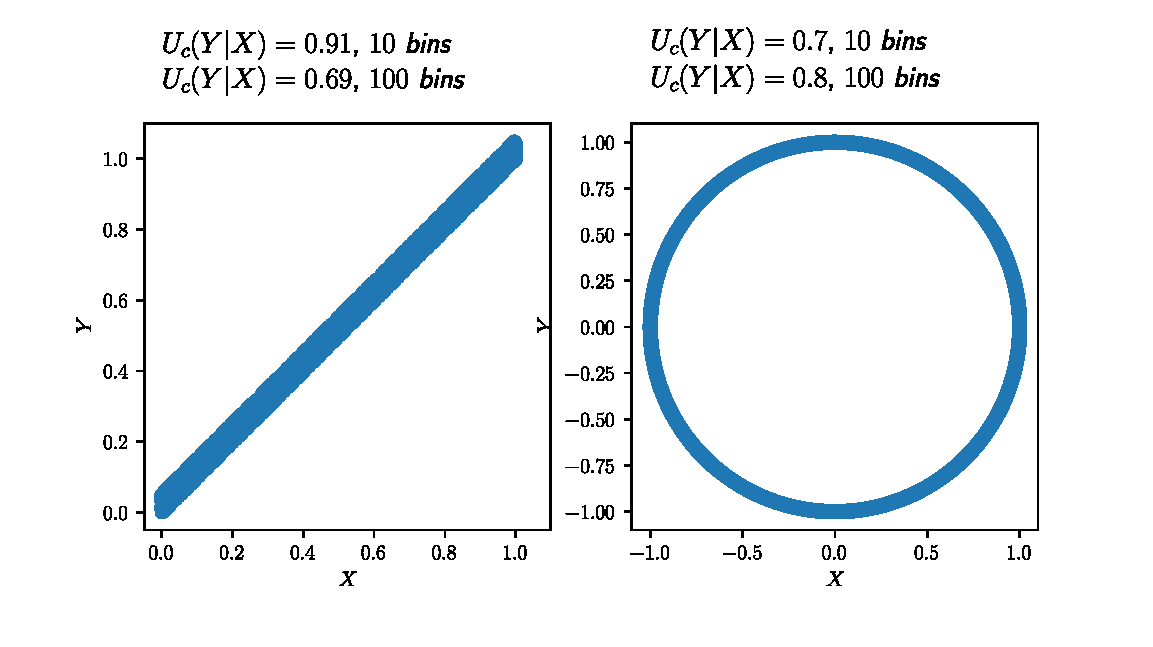
\includegraphics[width=0.75\textwidth]{comparaison_binning.pdf}
    \caption{Comparaison de la mesure du coefficient d'incertitude $U_c(Y|X)$ entre deux distributions. À gauche, la relation entre les variables $Y$ et $X$ est proche d'une fonction, bien qu'elle soit bruitée. À droite, la relation n'est pas fonctionnelle, mais telle qu'une valeur de $X$ correspond à exactement deux valeurs de $Y$. Dans les deux cas, $X$ est discrétisé en 500 \emph{bins}, et nous présentons les valeurs $U_c$ calculées pour des discrétisations de $Y$ en 10 et 100 \emph{bins}. Le choix de paramètre pour la discrétisation de $Y$ a un impact significatif sur la valeur du coefficient d'incertitude mesuré.}
    \label{fig:exemple-limite}
    \end{figure}

Afin de choisir ces paramètres d'estimation, décrivons le type de relation fonctionnelle que nous cherchons à mesurer dans une carte de l'architecture.
Nous présentons en figure~\ref{fig:exemple-limite} deux exemples de relations entre des variables aléatoires $X$ et $Y$. Dans le cas de gauche, la relation se rapproche d'une relation fonctionnelle, mais cette relation est bruitée. Une même valeur de $X$ correspond à un intervalle de valeurs de $Y$. Dans le cas de droite, la relation n'est pas une fonction, mais une valeur de $X$ correspond à exactement deux valeurs de $U$. En haut de la figure, nous indiquons le coefficient d'incertitude, calculé pour deux résolutions de discrétisation de $Y$: 100 \emph{bins} et 10 \emph{bins}. Dans les deux cas, $X$ est discrétisé en 500 \emph{bins}.


L'indicateur que nous voulons utiliser au sein de CxSOM doit privilégier la fonction bruitée (à gauche de la figure) par rapport à la relation qui n'est pas fonctionnelle (à droite).
Dans le cadre de l'analyse de CxSOM, nous cherchons en effet à mesurer si une valeur de $\bmu$ correspond à un unique intervalle de $U$. 
Dans le cas d'une carte simple, deux valeurs de $U$ éloignées sont en effet codées par une même position de BMU, voir figure~\ref{fig:cr_xp} plus bas.
Lorsque nous utilisons une discrétisation fine, par exemple de $100$ bins sur la figure, le coefficient d'incertitude calculé dans le cas ou la relation est non fonctionnelle est inférieur à celui calculé dans le cas de la relation fonctionnelle bruitée.
En effet, une valeur de $X$ correspond à seulement 2 valeurs de \emph{bins} pour $Y$ dans le cas du cercle, mais 10 dans le cas de la fonction bruitée. La proximité de ces points n'est pas représentée dans le calcul.
Lorsque nous élargissons la taille de discrétisation de $Y$, $U_c(Y|X)$ s'améliore dans le cas de la relation bruitée. Cette discrétisation à gros grain pour $Y$ permet d'ignorer la dispersion locale des valeurs de $Y$.

Pour que $U_c(U|\bmu)$ ne prenne pas en compte un bruit local sur les valeurs de $U$, il faudra donc choisir une discrétisation de $U$ à gros grains. Ces paramètres de discrétisation sont cependant à calibrer en fonction de l'organisation des données.
L'indicateur $U_c$ défini ici doit plutôt être considéré comme un indicateur statistique s'inspirant du coefficient d'incertitude que comme une estimation d'une valeur théorique, à cause de ce choix de paramètres et de la discrétisation des variables.

\subsection{Application du coefficient d'incertitude à CxSOM}

\begin{figure}
    \centering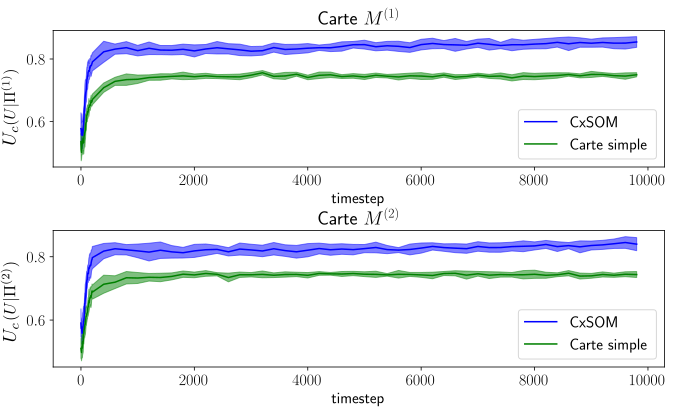
\includegraphics[width=0.8\textwidth]{evolution_MI_2}
    \caption{\'Evolution du coefficient d'incertitude $U_c(U|\bmu)$ dans chaque carte au long de l'apprentissage. L'intervalle de discrétisation choisi pour $U$ est de $0.02$ (50 \emph{bins}).
    La courbe bleue correspond à $U_c(U|\bmu)$ dans l'architecture de cartes $M\m{1}$ et $M\m{2}$, que nous comparons à l'évolution de $U_c$ dans une carte simple apprenant sur les mêmes entrées $\inpx\m{1}$ ou $\inpx\m{2}$. Les courbes correspondent à la moyenne et l'écart-type de $U_c$, calculés sur 10 expériences indépendantes.}
    \label{fig:MI_evol}
    \end{figure}

Nous traçons maintenant l'évolution de $U_c(U|\bmu)$ au cours de l'apprentissage dans un système de deux cartes apprenant sur le cercle en deux dimensions, afin de vérifier comment $U_c$ reflète la qualité de l'apprentissage du modèle dans une carte. 
Le tracé de $U$ selon $\bmu$ est représenté plus bas en figure \ref{fig:cr_xp}.

Pour cela, nous calculons $U_c(U|\bmu\m{1})$ et $U_c(U|\bmu\m{2})$ sur des phases de test réalisées tout au long de l'apprentissage d'une architecture de cartes. Nous effectuons en parallèle l'apprentissage de deux cartes simples apprenant l'une sur $\inpx\m{1}$ et l'autre sur $\inpx\m{2}$, sur laquelle nous calculons les mêmes indicateurs.
Leur évolution est tracée en figure~\ref{fig:MI_evol}.
Nous avons discrétisé $U$ en 50 \emph{bins}, et  $\bmu\m{i}$ en 500~: comme soulevé au paragraphe précédent, il est nécessaire d'utiliser un intervalle plus large pour les valeurs de $U$, afin de ne pas prendre en compte la dispersion des points au niveau local.

Ces tracés montrent que les quantités $U_c(U|\bmu\m{1})$ et $U_c(U|\bmu\m{2})$ sont bien toutes deux plus élevées pour CxSOM, tout au long de l'apprentissage, que dans le cas ou les cartes sont séparées. Les valeurs pour CxSOM s'approchent de 1 à la fin de l'apprentissage, reflétant bien que $U$ est une fonction de $\bmu$ dans chaque carte.

\subsection{Discussion}

D'après nos observations, $U_c$ peut certes être utilisé comme indicateur d'une relation fonctionnelle entre $U$ et $\bmu$ dans chaque carte, mais sous réserve de choisir correctement la taille de l'intervalle de discrétisation pour $U$ lors de l'estimation (nombre de \emph{bins})
La taille de cet intervalle de discrétisation doit être assez élevée pour englober un bruit local sur les $U$, mais l'intervalle doit rester suffisamment faible pour détecter une séparation entre deux intervalles de $U$ codés par une même position de BMU.
Le choix de cet intervalle de discrétisation de $U$ a une grande influence sur la valeur de l'indicateur, rendant difficile son utilisation comme valeur quantitative permettant de comparer des expériences.
Par ailleurs, la discrétisation de $U$ pour des variables de grande dimension nécessiterait un échantillon de grande taille, ce qui limite également son utilisation.
Enfin, l'aspect originellement continu des variables $\bmu$ et $U$ n'est pas pris en compte par cet indicateur, qui nécessite la discrétisation des variables.

Le coefficient d'incertitude n'est donc pas un indicateur adapté à la mesure de la relation fonctionnelle existant entre $U$ et $\bmu$. Bien qu'il s'appuie sur l'information mutuelle, qui mesure une relation quelconque entre des signaux, il ne traduit pas la relation fonctionnelle de la façon dont nous voulons la mesurer dans CxSOM. En particulier, nous voulons prendre en compte l'aspect continu des valeurs de $U$. Pour cela, nous étudions dans la suite le ratio de corrélation.

Cependant, l'utilisation de l'information mutuelle continue pour évaluer l'apprentissage nous paraît pertinente, mais afin d'évaluer une relation plus générale que la relation fonctionnelle.
Nous explorerons ce calcul en section~\ref{sec:mi}.

\section{\'Evaluation de la relation fonctionnelle entre $U$ et $\bmu$ par le ratio de corrélation}

Au vu des limitations montrées par l'indicateur $U_c$, nous avons choisi de considérer un autre indicateur de la relation fonctionnelle entre $U$ et $\bmu$~: le ratio de corrélation, qui s'appuie sur l'espérance conditionnelle de $U$ sachant $\bmu$.

\subsection{Définition}

Le ratio de corrélation $\eta(Y;X)$ est un coefficient mesurant une relation fonctionnelle non-linéaire entre deux variables. Il atteint la valeur de 1 lorsque $Y$ est fonction de $X$, et est nul lorsque les deux variables sont statistiquement indépendantes.

La mesure de la dépendance fonctionnelle entre deux variables $X$ et $Y$ peut se décomposer en deux étapes~:
\begin{enumerate}
    \item Trouver une fonction $\varphi(X)$ qui approxime les valeurs de $Y$
    \item Mesurer la qualité de l'approximation.
\end{enumerate}

La fonction approchant le mieux l'ensemble des valeurs $(x,y)$ d'un échantillon de deux variables $(X \in \Omega_X$, $Y \in \Omega_Y)$, au sens des moindres carrés, est la fonction~:
\begin{equation}
    \varphi(x) = \mathbb{E}(Y|X = x), x \in \Omega_X
\end{equation}

Le ratio de corrélation $\eta$ se définit à partir de $\varphi$ et mesure alors la qualité de l'approximation des valeurs de $Y$ par la fonction $\varphi$~:

\begin{equation}\label{eq:cr}
   \eta(Y;X) = \frac{Var(\mathbb{E}(Y|X))}{Var(Y)}
\end{equation}

Une possibilité d'estimation de $\varphi(x)$ est illustré en figure~\ref{fig:cr_box}~: nous discrétiserons les valeurs de $X$ en $n$ valeurs $(x_1, \cdots, x_n)$ et prendrons $\varphi(x_i)$ comme la moyenne des valeurs de $Y$ dans l'intervalle $[x_{i-1}, x_i]$.
Le ratio de corrélation n'est pas symétrique. Par le fait qu'il est construit sur un rapport, il n'est pas sensible à une transformation linéaire de $Y$ et est sans unité.

\begin{figure}
    \centering
    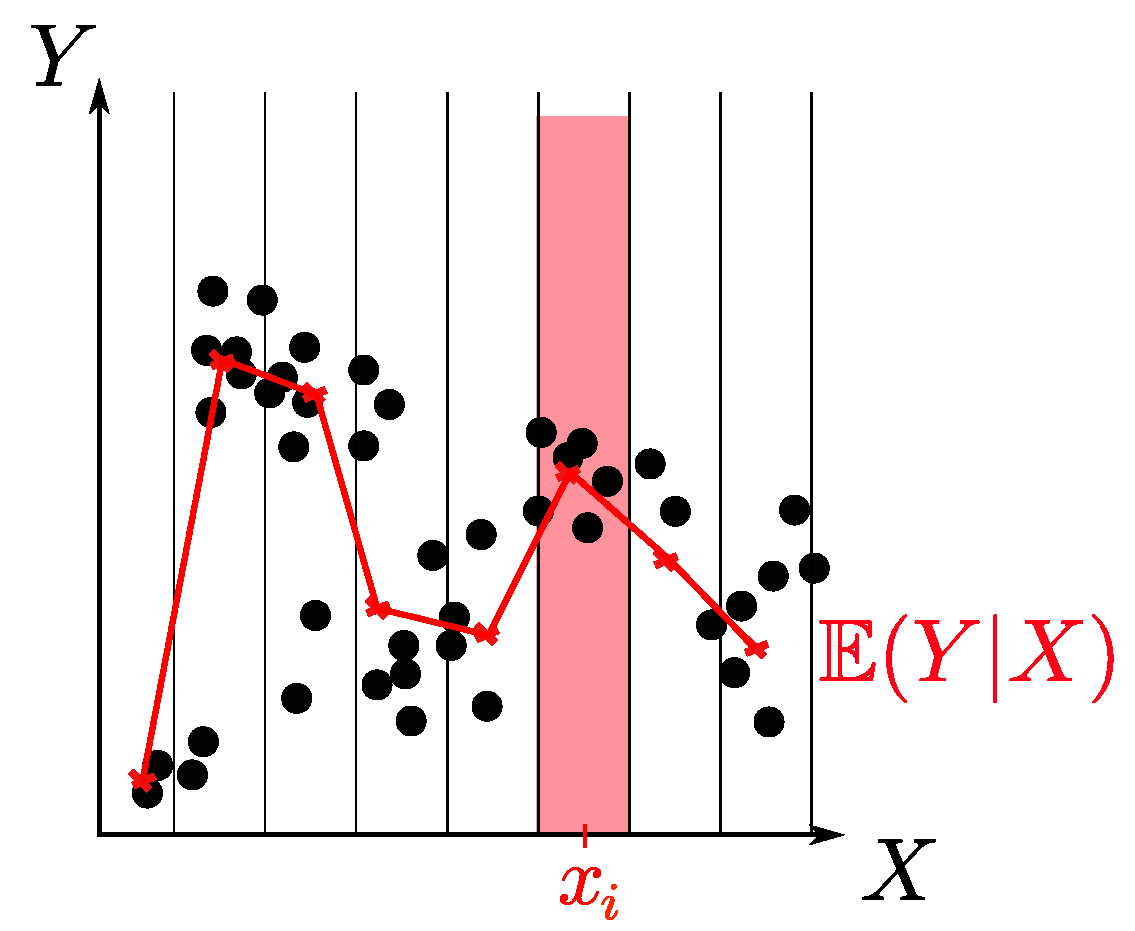
\includegraphics[width=0.5\textwidth]{boxes_CR.pdf}
    \caption{Exemple d'approximation non-linéaire de la relation entre $X$ et $Y$ par $\varphi(x)= \mathbb{E}(Y|X=x)$. Cette approximation est ici réalisée en discrétisant les valeurs de $X$. \label{fig:cr_box}}
\end{figure}

\subsection{Application du ratio de corrélation à CxSOM}

\begin{figure}
    \centering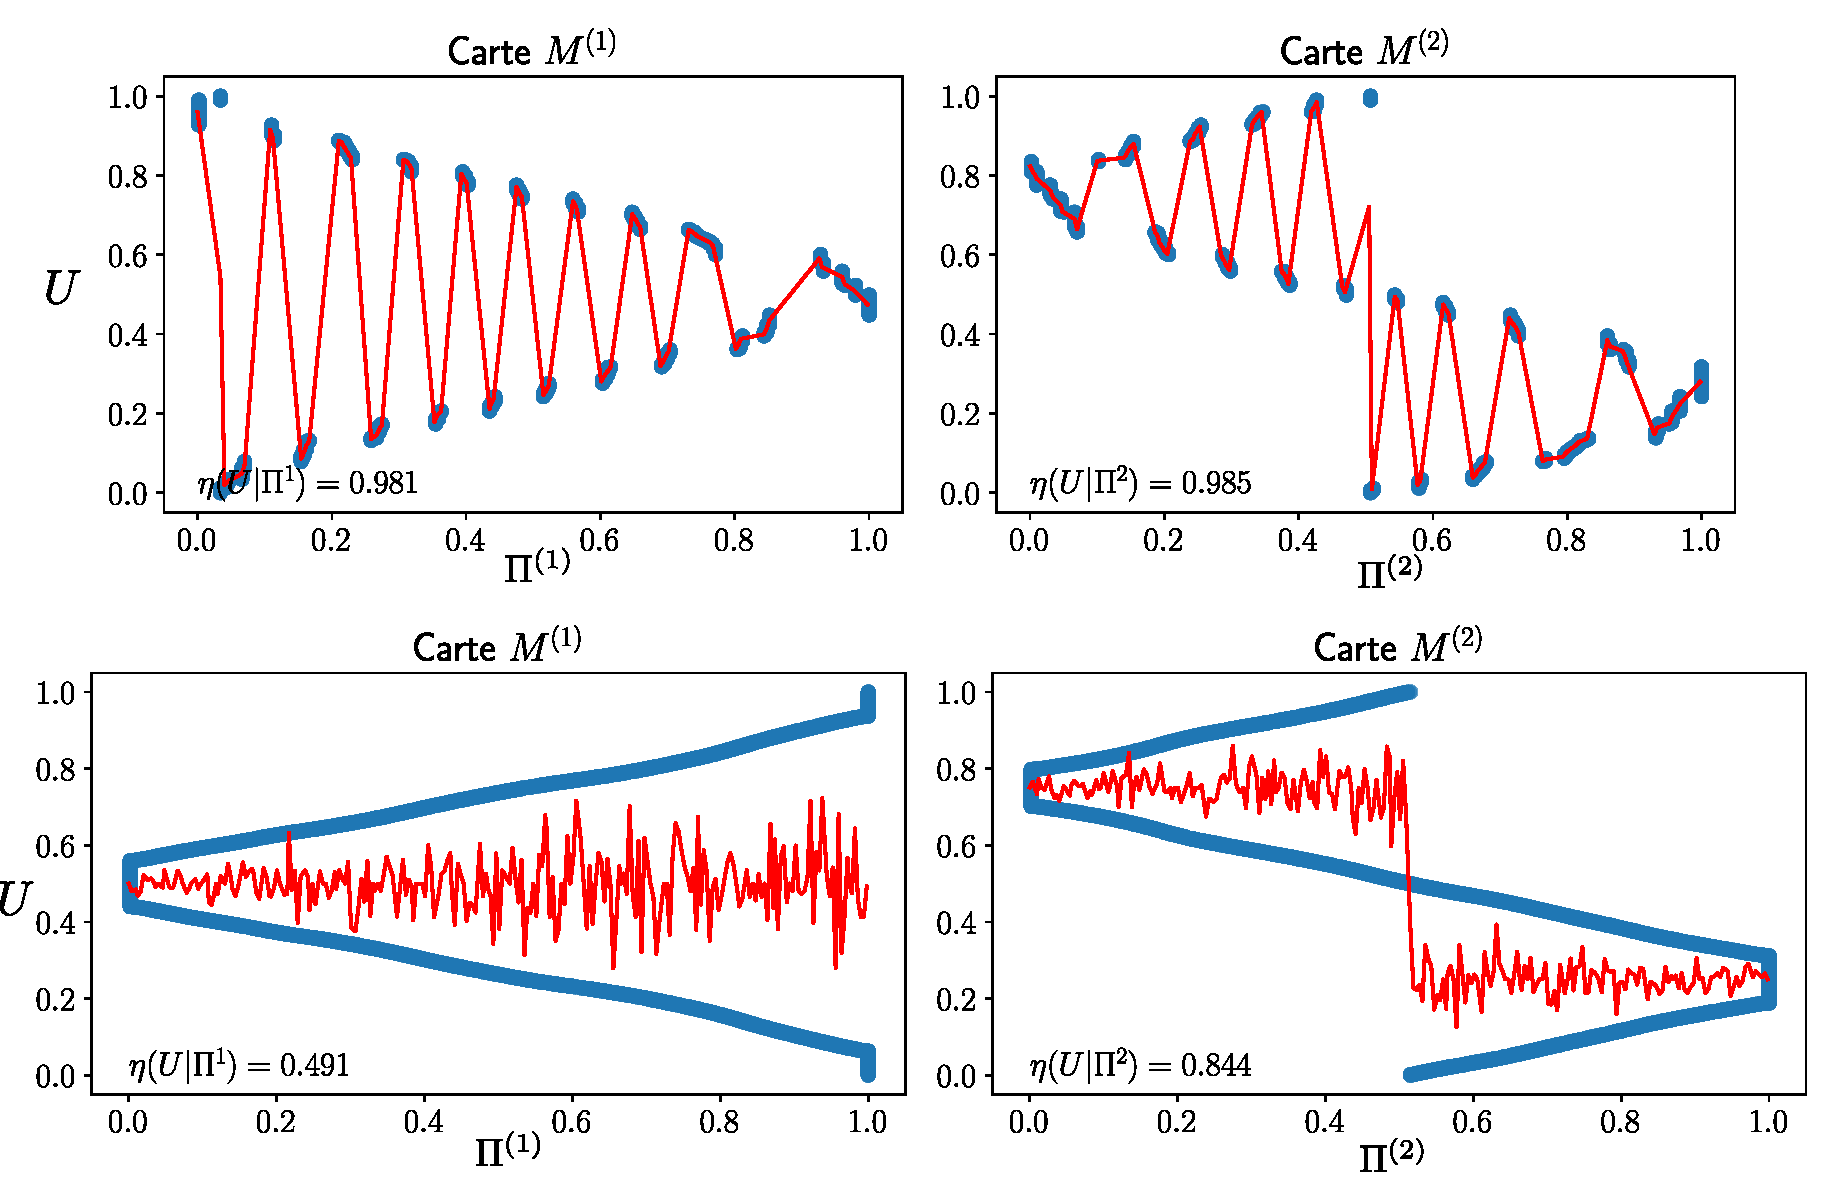
\includegraphics[width=0.8\textwidth]{correlation_ratio_cercle0.pdf}
    \caption{Tracé du ratio de corrélation et de $\varphi$ sur des entrées placées sur un cercle, dans le cas de CxSOM (en haut) et d'une carte simple (en bas). $\varphi(p) = \mathbb{E}(U|\bmu =p)$ est tracée en rouge.
    Nous observons que $\varphi(p)$ permet bien d'approximer la relation fonctionnelle entre $U$ et $\bmu$ dans chaque carte, en haut, ce qui se traduit sur la valeur du ratio de corrélation~: $\eta(U;\bmu\m{1}) = 0.98$, $\eta(U;\bmu\m{2}) = 0.99$. Au contraire, le ratio de corrélation est plus faible dans le cas des cartes simples, en bas.
     \label{fig:cr_xp}}
\end{figure}

\begin{figure}
   \centering 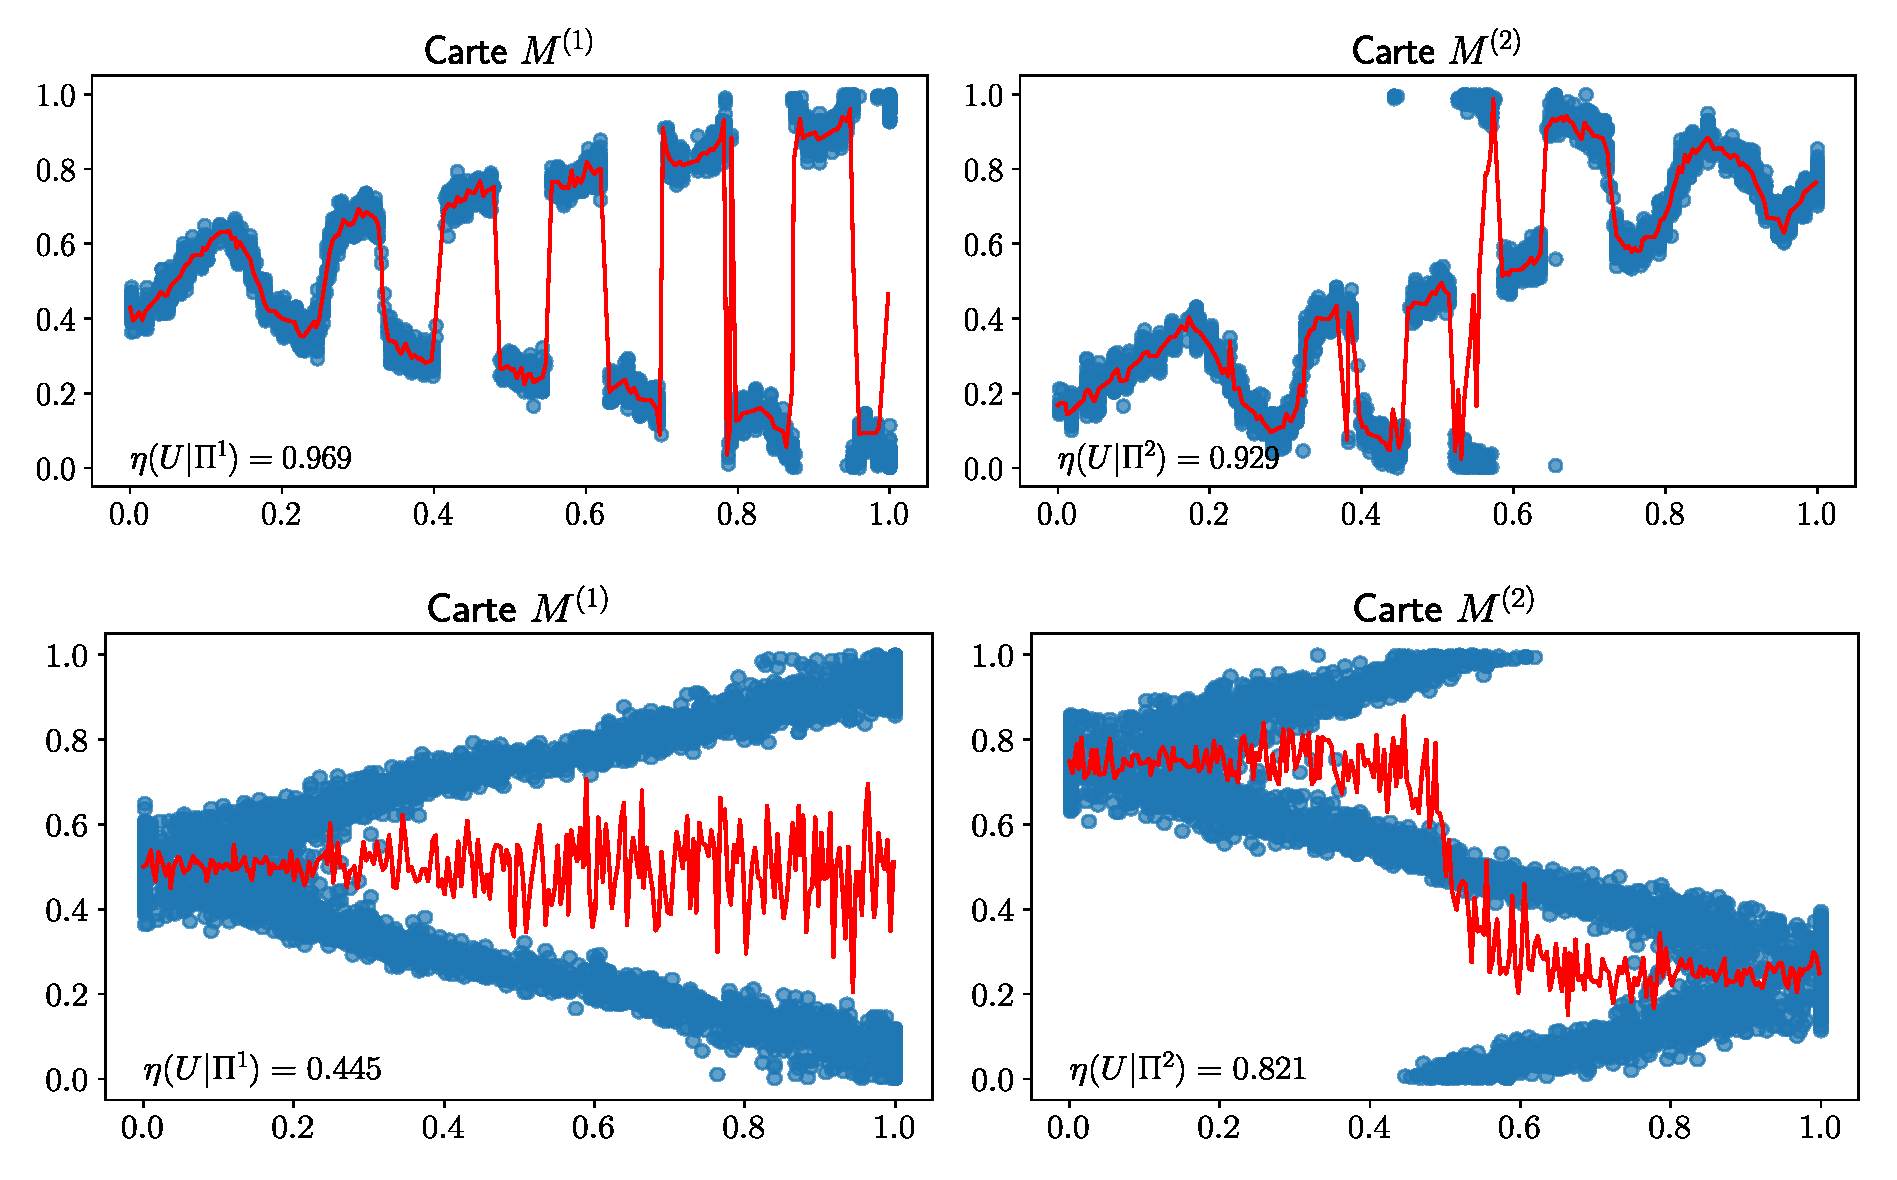
\includegraphics[width=0.8\textwidth]{xu_yu_both_anneau.pdf}
    \caption{Tracé du ratio de corrélation et de $\varphi$ sur des entrées placées sur un anneau, dans le cas de CxSOM (en haut) et d'une carte simple (en bas). Les données d'entrées sont bruitées, ce qui conduit à une dispersion plus élevée de $U$ pour chaque valeur de $\bmu$, tout en restant dans un seul intervalle. Le ratio de corrélation traduit toujours correctement que la relation entre $U$ et $\bmu$ s'approche d'une fonction et reste plus élevé que dans le cas des cartes simples. \label{fig:cr_bruit}}
\end{figure}

Nous utilisons à présent le ratio de corrélation pour quantifier la relation fonctionnelle entre $U$ et $\bmu\m{i}$, sur une architecture de deux cartes après apprentissage. Le but ici est d'illustrer comment cet indicateur traduit les observations réalisées graphiquement sur le modèle CxSOM, afin de valider son utilisation et de comprendre ce qu'il représente.

Nous reprenons trois exemples de modèles d'entrées tirés du chapitre précédent~:
\begin{itemize}
    \item Lorsque les entrées sont tirées sur le cercle de centre 0.5 et de rayon 0.5 (Entrées \textbf{A}, figure~\ref{fig:inputs}). $U$ correspond à l'angle du point sur le cercle.
    \item Lorsque les entrées sont tirées sur un anneau, construit en ajoutant un bruit aux points de centre 0.5 et de rayon 0.5. (Entrées \textbf{F}). $U$ correspond également à l'angle du point sur le cercle et l'indicateur doit pouvoir refléter l'apprentissage de $U$ malgré le bruit sur les entrées.
    \item Lorsque les entrées sont tirées sur une courbe de Lissajous (Entrées \textbf{D}). $U$ est le paramètre de la courbe.
\end{itemize}

Nous comparerons les valeurs du ratio de corrélation obtenues dans l'architecture, à celles obtenu dans le cas de deux cartes simples qui prennent $\inpx\m{1}$ ou $\inpx\m{2}$ en entrées. 
Dans ce dernier cas, les cartes ne présentent pas de relation fonctionnelle entre $U$ et $\bmu$.

Nous représentons d'abord le tracé de $U$ selon $\bmu$ dans chaque carte, après apprentissage, en figure~\ref{fig:cr_xp} pour le cercle et en figure \ref{fig:cr_bruit} pour l'anneau. (Voir figure~\ref{fig:u_bmu_lissa} pour la courbe de Lissajous).
Nous y traçons également la fonction $\mathbb{E}(U|\bmu)$, qui approxime le nuage de points par une fonction. 
Les valeurs des ratios de corrélation calculés dans chacun des cas sont indiqués au tableau~\ref{tab:eta}.
Nous y ajoutons les valeurs de $\eta(U;\inpx\m{1})$ et $\eta(U;\inpx\m{2})$, qui quantifient la relation initiale entre chaque entrée et $U$.


Nous observons sur les tracés que la relation fonctionnelle entre $U$ et $\bmu$ est bien approximée par $\mathbb{E}(U|\bmu)$ dans le cas de l'architecture de cartes. Les valeurs de $\eta(U;\bmu\m{1})$ et $\eta(U;\bmu\m{2})$ sont alors proches de 1. 
Dans le cas de l'anneau, $\mathbb{E}(U|\bmu)$ approxime bien la relation fonctionnelle, même bruitée, ce qui se traduit sur la valeur de l'indicateur qui reste élevée~: $\eta(U;\bmu\m{1}) = 0.96$ et  $\eta(U;\bmu\m{1}) = 0.94$. 
L'indicateur différencie donc bien le bruit local sur $U$, de l'existence de deux intervalles de valeurs séparés de $U$ pour une même position $\bmu$.

Dans le tableau, nous notons par contre que $\eta(U;\inpx\m{2}) \approx 0.8$ dans chacun des modèles d'entrées~; cette valeur est proche de $1$, alors que la relation n'est pas \og plus fonctionnelle \fg{} que celle existant entre $U$ et $\inpx\m{1}$, pour laquelle $\eta(U;\inpx\m{1}) \approx 0.4$. Intuitivement, on s'attendrait à ce qu'un indicateur prenne une valeur similaire pour $\eta(U;\inpx\m{1})$ et $\eta(U;\inpx\m{2})$. Cette observation suggère que la valeur seule du ratio de corrélation ne suffit pas à quantifier de manière absolue la qualité de la relation fonctionnelle.
Le ratio de corrélation apparaît donc comme un bon indicateur de la relation fonctionnelle entre $U$ et $\bmu\m{i}$, mais sa valeur devra être comparée à $\eta(U;\inpx\m{i})$ pour pouvoir l'interpréter.

\begin{table}
    \centering
    \caption{Comparaison des valeurs du ratio de corrélation sur plusieurs expériences.\label{tab:eta}}
    \begin{tabular}{*7c}
        \toprule
        & \multicolumn{2}{c}{Entrées} & \multicolumn{2}{c}{CxSOM} & \multicolumn{2}{c}{Cartes Simples} \\
        \cmidrule(lr){2-7}
         & $\eta(U;\inpx\m{1})$ & $\eta(U;\inpx\m{2})$  & $\eta(U;\bmu\m{1})$ & $\eta(U;\bmu\m{2})$  & $\eta(U;\bmu\m{1})$ & $\eta(U;\bmu\m{2})$ \\    
        \midrule
        Cercle &   $0.45 $    & $0.84$  &  $0.98$ & $0.99$ & $0.49$ & $0.84$      \\
        Anneau &  $0.43$      &  $0.83$      & $0.97$ & $0.93$ & $0.44$ & $0.82$ \\
        Lissajous &  $0.81$     &  $0.80$ & $0.96$ & $0.94$  & & \\
        \bottomrule
    \end{tabular}
\end{table}

Enfin, nous traçons en figure~\ref{fig:cr_evol} l'évolution du ratio de corrélation sur les 200 premiers pas d'apprentissage des cartes. 
Nous observons que $\eta(U;\bmu)$ garde une valeur élevée tout au long de l'apprentissage pour CxSOM.
Le ratio de corrélation ne traduit donc pas l'organisation des poids.
En effet, il ne prend pas en compte la proximité des positions. Deux valeurs discrétisées de $\bmu$ ont la même influence dans le calcul, qu'elles soient proches ou distantes dans la carte.
Or, chaque carte définit son BMU en fonction de $\inpx\m{1}$ et de son entrée contextuelle $\bmu\m{2}$, qui représente directement $\inpx\m{2}$, même au début de l'apprentissage. $U$ est donc une fonction du BMU dans chaque carte dès le début de l'apprentissage, ce qui est observé sur la courbe d'évolution.
Nous pourrions par exemple remplacer la discrétisation de $\bmu$ par une fenêtre glissante afin de mieux représenter la continuité des positions.

\begin{figure}
    \includegraphics[width=\textwidth]{cr_evol.pdf}
    \caption{\'Evolution du ratio de corrélation pendant l'apprentissage d'une architecture de deux cartes sur des entrées en cercle. Les tracés correspondent à la moyenne et l'écart-type du ratio, calculés sur 10 expériences. Le ratio de corrélation reste plus faible dans les cartes simples que dans les cartes CxSOM. Il garde une valeur élevée tout au long de l'apprentissage~: le ratio de corrélation ne traduit pas l'organisation des poids, mais vérifie seulement qu'une carte a bien un BMU différent pour chaque valeur de $U$. \label{fig:cr_evol}}
\end{figure}

\subsection{Discussion}

Nous cherchions un indicateur numérique permettant de quantifier l'encodage du modèle d'entrées dans chaque carte, afin de caractériser des expériences pour lesquelles $U$ est de grande dimension, et d'avoir une valeur numérique permettant de comparer plusieurs expériences et d'optimiser les paramètres de l'architecture.
Le ratio de corrélation $\eta(U;\bmu)$ est une mesure statistique qui exprime par définition la relation fonctionnelle existant entre $U$ et $\bmu$.Cette mesure nécessite de discrétiser les valeurs de $\Pi$, mais pas celles de $U$~; l'aspect continu de $U$ est donc bien traduit par $\eta$, contrairement à $U_c$.
Il est adaptable pour des cartes en 2D, ainsi que des $U$ en grande dimension car il repose seulement sur le calcul de moyennes sur $U$.
Il s'agit donc d'une mesure appropriée de la relation fonctionnelle entre $U$ et $\bmu$ dans chaque carte.
Cette relation fonctionnelle est caractéristique de l'apprentissage de la relation entre les entrées dans des architectures de deux et trois cartes.
Cependant, il faut noter que sa valeur devra être comparée à la valeur qu'il prend initialement dans le modèle d'entrées.

\section{Comment utiliser l'information mutuelle continue comme indicateur d'un apprentissage ?}

Le ratio de corrélation et le coefficient d'incertitude ont proposé deux manières différentes de mesurer le fait que $U$ est une fonction du BMU dans chaque carte.
Bien que le coefficient d'incertitude $U_c$ s'appuie sur l'information mutuelle, l'indicateur que nous avons présenté n'en est pas une véritable estimation, par la discrétisation à gros grains de $U$.

Sur des architectures à plus de trois cartes, il n'est pas certain, ni même souhaitable, que $U$ soit une fonction de la position du BMU dans toutes les cartes d'une architecture. Nous attendrions plutôt que la représentation de $U$ soit distribuée entre les cartes, tout en présentant de la redondance en terme d'information.
Nous envisageons donc dans cette section des perspectives d'utilisation de l'information mutuelle entre $U$ et les positions des BMU $(\bmu\m{1}, \bmu\m{2})$ pour analyser l'apprentissage du modèle dans une architecture de cartes.

\subsection{\'Evolution de l'information mutuelle entre $U$ et $\bmu$ au cours d'un apprentissage}\label{sec:mi}

\begin{figure}
    \centering\includegraphics[width=0.8\textwidth]{evolution_MI_K_2}
    \caption{\'Evolution de $I(U,\bmu)$ dans chaque carte au long de l'apprentissage, estimé par la méthode des KNN (cf.équation~\ref{eq:knn}).
    Sa valeur est moyennée sur 10 expériences. Nous comparons les valeurs obtenues dans une architecture CxSOM, en bleu, au cas d'une carte apprenant indépendamment sur les mêmes entrées $\inpx\m{1}$ ou $\inpx\m{2}$.
    Le même échantillon $U$ a été utilisé lors de chaque phase de test pour une même expérience.
    Nous observons que les positions des BMU d'une carte indépendante partagent plus d'information avec $U$ que dans le cas de CxSOM.
    \label{fig:MI_evol_total}}
    \end{figure}

Nous nous intéressons à l'information mutuelle continue entre $U$ et $\bmu$, que nous estimons grâce à la méthode des KNN, présentée en section~\ref{sec:estimation}. Contrairement à l'estimation à gros grains réalisée en section précédente pour $U_c$, il s'agit maintenant d'une véritable estimation de la valeur de l'information mutuelle entre les deux variables continues que sont $\bmu$ et $U$.

En figure~\ref{fig:MI_evol_total}, nous traçons l'évolution de l'information mutuelle dans les deux cartes au cours de phases de test réalisées tout au long de l'apprentissage.
Nous observons que l'information mutuelle entre $U$ et $\bmu$ évolue vers une valeur qui est plus élevée dans une carte isolée que dans une architecture CxSOM.
Ce résultat est étonnant~: cela signifie que chaque carte au sein de CxSOM encode en fait moins d'information sur le modèle d'entrées qu'une carte indépendante, qui ne reçoit pourtant que l'entrée $\inpx\m{1}$ ou $\inpx\m{2}$.
Notre interprétation de ce résultat est que l'information apprise sur le modèle par une carte n'est pas répartie de la même façon dans les deux expériences.
Dans une carte indépendante, le niveau de quantification vectorielle sur $\inpx$ est plus précis que celui que nous avions observé dans CxSOM.
Or, l'encodage de la valeur $\inpx$ donne déjà beaucoup d'information sur le modèle $U$.
Dans CxSOM, on perd ce niveau de quantification sur $\inpx$, ce qu'on a observé en figure~\ref{fig:erreur}. On perd donc de l'information sur $\inpx$.
% Le fait que l'information mutuelle soit plus élevée dans une carte indépendante dans les deux expériences traduirait ainsi une perte d'information sur l'entrée $\inpx$ dans CxSOM par rapport à une carte simple, à cause de la perte de précision en quantification vectorielle. 
La valeur de l'information mutuelle comprend à la fois le gain d'information qui existe sur $\inpx\m{2}$ au sein de $M\m{1}$, donc sur $U$ (et inversement), et la perte d'information sur $\inpx\m{1}$. 
Il est probable que cette perte d'information domine dans le calcul, d'où la perte globale d'information.
Les cartes effectueraient donc un compromis~: chacune gagne de l'information sur le modèle $U$, au détriment de l'information apprise sur l'entrée externe.

Afin de mieux analyser l'apprentissage du modèle d'entrées par les cartes, nous pouvons envisager des méthodes permettant de séparer l'information entre variables. Elles nous permettraient de mesurer le gain d'information sur $U$ dans une ou plusieurs cartes sans s'intéresser à l'information gagnée ou perdue sur l'entrée externe $\inpx$.
Nous avions en fait utilisé une méthode de séparation de cette information lors de l'estimation du coefficient d'incertitude $U_c$~: le fait de discrétiser grossièrement la distribution de $U$ a permis de mesurer le gain d'information sur $U$, sans prendre en compte l'affaiblissement de la précision de la quantification de l'entrée externe.

Cette perte d'information pose néanmoins une question concernant la création d'architectures contenant de nombreuses cartes, sur des modèles d'entrées pour lesquels $U$ est de grande dimension~: jusqu'à quel point une carte peut-elle se permettre de perdre de l'information sur l'entrée externe pour gagner de l'information sur le modèle ? 
Cette observation renforce l'idée que l'encodage d'une variable $U$ en grande dimension dans une architecture devra être distribué entre les cartes. D'après les seules observations réalisées sur deux et trois cartes dans cette thèse, nous ne pouvons pas affirmer ou non si cette propriété sera vérifiée, en raison de la taille de l'architecture.
Cela constitue une perspective de travaux futurs pour le développement du modèle.

\subsection{Perspectives possibles}

\begin{figure}
    \centering\includegraphics[width=0.5\textwidth]{redondance}
    \caption{Illustration des notions d'information \emph{redondante} et \emph{synergique} entre une variable $S$ et deux variables $R_1$ et $R_2$, schéma adapté de \cite{williams_nonnegative_2010}. Ces travaux définissent une façon de séparer l'information que portent des variables $R_1$ et $R_2$ sur une source $S$. La redondance est l'information apportée à la fois par $R_1$ et $R_2$; la synergie est celle qui n'est apportée que par leur jointure $(R_1,R_2)$. \label{fig:redondance}
    }
\end{figure}

Les indicateurs proposés dans ce chapitre ont permis d'évaluer un apprentissage du modèle indépendamment dans chaque carte. 
Les possibilités de mesure de l'information mutuelle dans une architecture de cartes ne se limitent pas au calcul de $I(U,\bmu)$~; d'autres indicateurs semblent intéressants à explorer pour une meilleure compréhension de l'apprentissage du modèle dans des architectures comportant plus de cartes.

Nous pouvons tout d'abord noter que la méthode d'estimation par KNN présentée dans ce chapitre est une méthode classique d'estimation de l'information, mais il existe de nombreuses autres méthodes \parencite{Doquire2012ACO}. Des méthodes ont également été développées pour la mesure de l'information mutuelle entre variables continues et discrètes \parencite{ross_mutual_2014, Gao2017EstimatingMI}. Enfin, l'information mutuelle a été utilisée pour analyser l'apprentissage de réseaux de neurones profonds en \cite{ShwartzZiv2017OpeningTB} ou encore directement comme métrique d'apprentissage en \cite{Hjelm2018LearningDR}.
Cette grandeur est ainsi bien documentée et donc pertinente à utiliser dans des travaux futurs.

Ensuite, nous avons soulevé le besoin de séparer les sources d'information sur $U$ et d'étudier son encodage distribué dans l'architecture. Il serait possible de s'intéresser à la notion d'information mutuelle multivariée~: étant donné une variable cible $S$ et deux variables $R_1$ et $R_2$, $I(S;R_1,R_2)$ désigne l'information mutuelle entre $S$ et la variable jointe $(R_1,R_2)$. 
Nous pourrons par exemple mesurer $I(U; \bmu\m{1}, \bmu\m{2})$.
Il est également possible de décomposer cette information multivariée~: \cite{williams_nonnegative_2010} définit, en plus de l'information mutuelle, les notions de redondance et de synergie entre variables, illustrées en figure \ref{fig:redondance}.
La redondance est l'information sur $S$ portée à la fois par $R_1$ et par $R_2$, et la synergie l'information portée seulement par la jointure des variables $R_1$ et $R_2$. Le calcul de telles grandeurs permettrait de séparer l'information gagnée sur $U$ et $\inpx$ dans une carte.
Le calcul de ces quantités entre les entrées, le modèle d'entrées et les BMU des cartes CxSOM est donc une piste d'étude pour une compréhension de l'encodage de l'information dans une architecture de cartes et pour la définition d'un indicateur ciblant spécifiquement le gain d'information sur $U$ lors de l'apprentissage.


\section{Conclusion}

Ce chapitre utilise la méthode de représentation des éléments des cartes comme des variables aléatoires présentée au chapitre \ref{chap:repr} pour proposer des indicateurs de l'apprentissage multimodal au sein de l'architecture.
Les représentations visuelles sont en effet limitées dans des architectures de plus de deux ou trois cartes, et pour des données en plus grande dimension. La définition d'un indicateur permettra également de comparer l'apprentissage d'architecture, autorisant par exemple l'optimisation automatique des paramètres de l'architecture de cartes.

Nous avons introduit deux indicateurs permettant de mesurer que $U$ est une fonction de $\bmu$ dans chacune des cartes de l'architecture~: le ratio de corrélation $\eta(U;\bmu)$ et le coefficient d'incertitude $U_c(U|\bmu)$.
Nous avons en effet observé dans les deux chapitres précédents que cette relation fonctionnelle marque l'apprentissage du modèle dans des architectures de deux ou trois cartes en une dimension.
Le coefficient d'incertitude est une version normalisée de l'information mutuelle. Il doit être estimé par histogrammes et est donc très sensible aux paramètres d'estimation, ce qui rend son utilisation peu adaptée comme indicateur. De plus, la discrétisation de $U$ est difficilement réalisable pour des variables de grande dimension.
Le ratio de corrélation permet de mesurer directement la relation fonctionnelle entre $U$ et $\bmu$, en passant par l'estimation de $\mathbb{E}(U|\bmu)$.
Dans un but de mesure de la relation fonctionnelle entre $U$ et $\bmu$, nous avons observé que le ratio de corrélation est à privilégier, car il est estimable pour des valeurs de $U$ en toute dimension et ne dépend pas de la taille d'intervalle choisie pour $U$. Sa valeur devra cependant être comparée aux valeurs du ratio de corrélation sur les données d'entrée $\eta(U;\inpx)$.

La relation fonctionnelle entre $U$ et $\bmu$ n'est toutefois pas une propriété souhaitable dans des plus grandes architectures ou pour des $U$ de plus grande dimension, car elle semble être accompagnée d'une forte perte d'information sur l'entrée externe au profit d'un grain d'information sur le modèle.
On voudrait plutôt que la représentation de $U$ soit distribuée entre les cartes.
Pour étudier l'apprentissage associatif dans un cadre plus général, nous suggérons aux travaux futurs de s'intéresser à des mesures d'information mutuelle multivariée entre $U$ et toutes les valeurs des BMU $(\bmu\m{1}, \cdots, \bmu\m{n})$ au sein des architectures de cartes.

Finalement, ce chapitre montre que la représentation des éléments d'une carte et des entrées comme variables aléatoires, que nous avons proposée au chapitre \ref{chap:repr}, est une méthode pertinente pour la compréhension des comportements d'apprentissage du modèle CxSOM.
Cette approche \og comportementale \fg{}, et non basée sur les poids des cartes, rapproche l'étude des cartes de Kohonen et de CxSOM des algorithmes d'apprentissage supervisés, dont les entrées et sorties sont bien définies.
Les représentations proposées et les perspectives d'études par l'information mutuelle mentionnées ci-dessus sont donc générales aux SOMs et à d'autres types d'architectures d'apprentissage. 

\ifSubfilesClassLoaded{
    \printbibliography
    %\externaldocument{../main.tex}   
}{}
\end{document}


% Nous avons observé que l'apprentissage du modèle dans deux et trois cartes se caractérise par le fait que chaque carte dissocie les BMU en fonction du modèle d'entrées $U$ et non seulement de son entrée externe. 
% La variable cachée $U$, représentant le modèle d'entrées, est alors une fonction du BMU $\bmu$ dans chacune des cartes de l'architecture, comme rappelé sur la figure~\ref{fig:upi_chap4}.
% Nous souhaitons définir un indicateur numérique caractérisant cette propriété, c'est-à-dire caractérisant que $U$ est fonction de $\bmu$ dans chaque carte. 

% Nous avons défini les expériences en termes de variables aléatoires. La théorie de l'information de Shannon \cite{Shannon1948AMT} apporte un modèle mathématique qui permet de manipuler et encoder ces variables et quantifier l'information partagée entre leurs distributions.
% Nous proposerons dans ce chapitre des indicateurs permettant d'évaluer l'apprentissage du modèle par l'architecture de cartes. 
% $\mathbb{E}(Var(Y|X))$ représente la moyenne des écarts de $Y|X=x_i$ à sa valeur moyenne en $x_i$ $\mathbb{E}(Y|X=x_i)$ pour une valeur de $X = x_i$ donnée. 
% En effet, en notant $Z$ la variable aléatoire $Y | X=x_i$~: 
% $$ Var(Y|X=x_i) = \mathbb{E}((Z - \mathbb{E}(Z))^2)$$
% $$ Var(Y|X=x_i) = \mathbb{E}((Z - \varphi(x_i))^2)$$

% Lorsque la dépendance entre $Y$ et $X$ est fonctionnelle, les valeurs de $Y|X = x_i$ sont très proches de $\varphi(x_i)$  pour toutes les valeur de $x_i$ et $\mathbb{E}(Var(Y|X=x_i))$ est faible partout. La variance est nulle lorsqu'une valeur de $X$ correspond à un seul point pour $Y$, c'est-à-dire une relation fonctionnelle. 
% Inversement, quand $Y$ et $X$ sont indépendantes, $Var(Y|X=x_i) = Var(Y)$ pour tout $x_i$, donc $\mathbb{E}(Var(Y|X)) = Var(Y)$ et $\eta(Y;X) = 0$.

% La définition du coefficient se retrouve plus généralement sous une forme modifiée de l'équation~\ref{eq:cr}~:
% par la définition des variances conditionnelles,
% $$Var(Y) = \mathbb{E}(Var(Y|X)) + Var(\mathbb{E}(Y|X))$$
% Soit~:
% \begin{equation}
%     \eta(Y;X) = \frac{Var(\mathbb{E}(Y|X))}{Var(Y)}
% \end{equation}
\documentclass[../main]{subfiles}
\ifSubfilesClassLoaded{
    \dominitoc
    \tableofcontentsfile
	\pagenumbering{arabic}
    \setcounter{page}{1}
	\addbibresource{../Biblio/biblio.bib}
}{}
\begin{document}
\chapter{Analyse de l'auto-organisation de CxSOM sur des cartes en une dimension}\label{chap:analyse}
\graphicspath{{06-Analyse/figures},{./figures}}
\minitoc

Nous avons proposé un modèle de connexions de cartes auto-organisatrices au sein d'une architecture complète s'appuyant sur un consensus~; le but de ce chapitre est de définir et comprendre des mécanismes d'auto-organisation occurrant dans des cartes en une dimension et permettant d'apprendre une relation entre entrées multimodales.
Nous conclurons sur la scalabilité du modèle à des architectures comportant un plus grand nombre de cartes. Nous généraliserons au chapitre suivant pour des cartes en deux dimensions.

\section{Méthode expérimentale}

Nous utiliserons en premier lieu des modèles géométriques d'entrées. Ces modèles nous permettent de maîtriser les dépendances sur des modalités en basse dimension et ainsi de visualiser les liens entre organisation et apprentissage. Cela nous permettra également de mesurer l'apprentissage de cette dépendance connue au sein des structures de cartes.

\subsection{Entrées géométriques}

La dépendance entre modalités est définie par la dimension choisie pour $U$.
Une variable $U$ en une dimension paramètre des points placés sur une courbe en une dimension~; $U$ en 2 dimensions paramètre une surface 2D. 
Plus généralement, quelle que soit la dimension totale $n$ des entrées, nous prendrons ces entrées placées sur une variété de dimension inférieure, $k$,  définie par $U \in [0,1]^k$ et qui définit la dépendance entre entrées. 
Ce modèle est général~: au pire, $U$ correspond à la dimension totale des entrées. Par ailleurs, de nombreux modèles d'entrées réelles se placent sur une variété (\emph{manifold}) de dimension réduite, comme nous l'avions vu au chapitre \ref{chap:repr} pour des images d'un même objet 3D vu par différents angles. Le choix d'un modèle d'entrées géométriques situées sur une variété de dimension inférieure est donc justifié comme modèle expérimental simplifié.
Nous considérons d'abord des points pour lesquels $U$ est en une dimension~: ils sont situés sur une courbe. 
Nous reviendrons d'abord  sur les conclusions de l'expérience présentée au chapitre représentation, sur des données disposée en cercle (A). L'intérêt de cette courbe est que la disposition est symétrique~: toute entrée $X^{(1)}$ correspond à deux valeurs possibles pour $X^{(2)}$ et inversement.
Nous testerons ensuite si les observations réalisées sur cette disposition d'entrées se retrouve dans d'autres dispositions listées ci-dessous, représentées en figureé\ref{fig:input_list}~:
\begin{itemize}
	\item Une entrée est fonction de l'autre~: $\inpx\m{2} = cos(\inpx\m{1})$~(\textbf{B})
	\item Entrées identiques (cas dégénéré). Ces points sont toujours sur une courbe 1D, mais leur dépendance est bijective.~(\textbf{C})
	\item Courbe de Lissajous (D).
	\item Entrées totalement indépendantes, prises aléatoirement dans un carré $[0,1]^n$~(\textbf({E}))
	\item Une carte de Kohonen classique a comme propriété d'être résistante au bruit des données. Ainsi, une carte 1D se dépliant sur un anneau fin en 2D apprendra d'abord la représentation du cercle. Nous voulons vérifier comment cette propriété se vérifie sur l'apprentissage de données par plusieurs cartes~; nous prendrons ainsi des points sur un anneau \textbf{(F)}
\end{itemize}

Nous étudierons l'organisation après apprentissage de structures de deux cartes connectées réciproquement, sur ces différents jeux d'entrées, comme proposé au chapitre \ref{chap:repr} et tracerons les représentations. 
Dans un premier temps, nous étudions des architectures de deux cartes 1D, ce qui nous permettra de mieux comprendre certains mécanismes d'organisation.
Nous étendrons ensuite notre étude à des architectures de 3 cartes en une dimension, toutes connectées. 
% Nous appliquerons ces architectures à une courbe ($U$ 1D) mais sur trois dimensions, chacune des cartes prenant une des dimensions d'un point comme entrée \ref{fig:cercle3}. Il s'agit ici d'un cercle en deux dimensions que nous pivotons sur la troisième dimension. De cette manière, il existe une redondance entre $X\m{1}, X\m{2}$ et $X\m{3}$ : étant donné $X\m{1}, X\m{2}$ et le modèle d'entrée, il est possible d'en déduire l'entrée manquante.
Dans ce cadre, nous réaliserons de la prédiction d'entrée par les cartes. Nous donnons en entrées $X\m{1}, X\m{2}$ à la structure et verrons si la valeur de $X\m{3}$ correspondante est correctement prédite par l'architecture. Une bonne prédiction témoignera de l'apprentissage du modèle d'entrées par l'architecture de cartes.
Les architectures de cartes en deux dimensions seront traitées par la suite au chapitre~\ref{chap:analyse2D}.

\begin{figure}
	\includegraphics[width=\textwidth]{inputs/inputs.pdf}
	\caption{Dispositions d'entrées en deux dimensions. $M\m{1}$ prend en entrée l'ordonnée $\inpx\m{1}$ et $M\m{2}$ prend en entrée l'abscisse $M\m{2}$. \label{fig:input_list}}
\end{figure}

\subsection{Matériel}

Les expériences présentées ici ont été développées en C++ en s'appuyant sur la librairie CxSOM \footnote{\url{https://github.com/HerveFrezza-Buet/cxsom}}, développée au sein de notre équipe.
Cette librairie permet d'implémenter des cartes de Kohonen simples ainsi que des architectures CxSOM par le modèle que nous avons présenté.
Cette librairie s'interface avec python par un module pycxsom afin de faciliter les représentations et manipulation des cartes pendant et après l'apprentissage. Elle cherche à paralléliser au maximum les opérations indépendantes. Par exemple, la phase d'apprentissage des cartes reste séquentielle car le calcul des valeurs des poids pour l'itération $i$ dépend de $i-1$, mais toutes les opérations de tests dans lesquelles le temps n'intervient pas tournent en parallèle.
Notons que la gestion du consensus lors de la relaxation passe également par des mécanismes locaux aux cartes dans notre implémentation. Nous devons en effet vérifier lors de chaque pas de relaxation si les cartes ont atteint un consensus. Pour cela, chaque carte envoie un signal supplémentaire aux cartes voisines indiquant si son BMU a été modifié. Lorsque qu'une carte reçoit de toutes ses voisines que leur BMU n'est plus modifié et que le BMU de la carte n'a pas non plus été modifié lors de l'étape, la relaxation s'arrête dans cette carte.

Les codes C++ et python que nous avons utilisé pour générer les expériences présentées dans ce chapitre sont disponible sur git : REF.
Toutes les expériences présentées ici tournent sur un simple processeur i7.

\subsection{Paramètres et architectures}

Chaque jeu de donnée sert d'entrée d'apprentissage à une architecture de deux cartes 1D connectées réciproquement. Chaque carte a une taille fixée de 500 unités, indexées entre 0 et 1, et possède deux couches de poids $\w_e$ et $\w_c$. Les rayons de voisinage sont d'abord choisis à $r_e = 0.2$ et $r_c = 0.02$.
La génération des entrées suit le processus suivant~: $U$ est tiré uniformément dans $[0,1]$, puis les entrées $\inpx\m{1}$ et $\inpx\m{2}$ sont ensuite calculées à partir de la valeur de $U$.
L'apprentissage est réalisé sur un échantillon de 20000 itérations, générés aléatoirement. Les tests sont ensuite réalisés sur 1000 points générés aléatoirement selon la même distribution.

\section{Résultats}

Le premier but de cette étude est d'identifier des comportements \emph{systémiques} émergeant d'une architecture simple à deux et trois cartes, sur des entrées en deux et trois dimensions.
Nous avons identifié certains comportements au chapitre précédent, que nous évaluerons sur d'autres données entrées. Nous rappelons d'abord les comportements qu'on peut attendre d'une architecture de cartes.

\subsection{Entrées disposées sur un cercle : formulation d'hypothèses}

Revenons sur l'expérience précédemment présentée au chapitre \ref{chap:representation}, réalisée sur des entrées disposées selon un cercle. Nous avons alors relevé plusieurs comportements se différenciant de ce qu'on aurait pu voir avec une carte classique. Cette expérience a l'avantage d'être un cas de figure très simple d'entrées multimodales.

\subsubsection{Convergence des poids}

Dans une carte de Kohonen classique, le rayon de voisinage et le taux d'apprentissage sont décroissants au cours des itérations. Cette opération permet d'assurer un dépliement des cartes au début de l'apprentissage puis assure la convergence des poids $\w$ des cartes lorsque les paramètres décroissent.
Dans notre étude, nous choisissons de ne pas modifier les paramètres d'apprentissage au cours des itérations.
Sans chercher à démontrer mathématiquement une convergence des poids, déjà difficile à démontrer sur des cartes de Kohonen classique, nous pouvons évaluer expérimentalement la convergence des poids au cours de l'apprentissage.
La figure~\ref{fig:conv} présente l'évolution de la modification des poids $\w\ext$ et $\w\cont$ dans chaque carte au cours de l'apprentissage. La différence considérée ici est $||\w_t - \w_{t-1}||_{\infty}$ (maximum sur les positions $p$ des différences entre les valeurs des poids $\w$ à l'instant $t$ et l'instant $t-1$). Ce calcul de différence est moyenné pour 10 expériences, chacune lancée sur des entrées aléatoires tirées de la même distribution sur le cercle, pour une initialisation aléatoire des poids des cartes.
Nous observons que cette courbe tend vers $0$ pour chaque courbe de poids, donc que tous les poids tendent vers une position stable.

Cette convergence est favorisée par la différence de contribution dans l'activité globale des activations externes et contextuelles, calculée, rappelons le, par~: 
$$ a_g = \sqrt{a_e \cdot (\beta a_e + (1-\beta)a_c)}$$
La carte se comporte donc d'abord comme une carte de Kohonen classique apprenant sur des entrées externes, qui pour des cartes 1D sur des entrées 1D converge sans problème même en l'absence de décroissance des paramètres d'apprentissage. Les entrées contextuelles viennent seulement moduler un peu le calcul d'activité.

Notons toutefois que nous sommes sur un cas particulier de cartes 1D sur des entrées 1D.
Nous verrons que la convergence en l'absence de décroissance de paramètres pose plus de problèmes sur des cartes en deux dimensions, comme il y a plus de configurations possibles pour la carte~; mais nous verrons aussi que pour des rayons de voisinage bien choisis, la convergence sera assurée également en deux dimensions.

\begin{figure}
	\includegraphics[width=\textwidth]{convergence/cercle_moy.pdf}
	\caption{Pour chaque carte, nous représentons l'évolution en fonction du temps d'apprentissage, de la différence maximale en valeur absolue entre les poids à l'instant $t$ et ceux à $t-1$ $\w_t$ et $\w_{t-1}$. Les entrées sont ici un cercle en deux dimensions. L'évolution est moyennée sur 10 apprentissages initialisés aléatoirement.
	Ces tracés montrent que les poids externes et contextuels convergent rapidement vers une position stable.\label{fig:conv}}
\end{figure}



\subsubsection{Disposition des poids}

Analysons maintenant la forme des poids contextuels de $M\m{1}$, tracés en figure~\ref{fig:w}.
Les poids externes, en orange, présentent une disposition similaire à ceux observés dans une carte classique. Les poids contextuels, en bleu, présentent une forme de vagues. Nous ajoutons à ces deux courbes le tracé des valeurs des entrées selon la position de leur BMU, en vert et rose sur la figure.

On remarque d'abord que les positions dans la carte $M\m{1}$ se répartissent en zones de BMUs, séparées par des zones mortes dans lesquelles aucune entrée n'a gagné. 
C'est une première différence avec une carte classique, pour laquelle toutes les positions seront BMUs lorsque les entrées sont distribuées de façon continue.
Les zones dans lesquelles il y a des BMUs correspondent aux extremum des poids contextuels et leurs alentours.

Dans la carte $M\m{1}$, les entrées externes $\inpx\m{1}$ sont proches de la courbe de poids externes, mais avec plus d'erreur de quantification que ce qu'on attendrait dans une carte simple. Une quantification vectorielle correcte est souhaitable, car elle permet de lier de retrouver la valeur de l'entrée à partir de la réponse d'une carte.
Nous notons que les zones définies par les poids contextuels partagent les positions des BMUs en fonction de la valeur des entrées. 
Deux points ayant la même valeur de $\inpx\m{1}$ mais une valeur différente de $\inpx\m{2}$ auront BMU différent dans la carte $M\m{1}$~; ces BMUs sont alors situées dans deux zones adjacentes.

Ainsi, une carte connectée au sein d'une architecture CxSOM différencie les échantillons en fonction de non seulement leur entrée externe, mais aussi de l'entrée de l'autre carte de l'architecture. La plage de valeurs des $\inpx\m{1}$ gagnant dans un des zones recoupe les plages de valeurs gagnant dans les zones situées à gauche et à droite. Par exemple, la zone dans laquelle l'échantillon rouge gagne, autour de $\bmu\m{1} = 0.25$. La partie des entrées située en dessous de la courbe de poids externe recoupe les valeurs d'entrées gagnant dans la zone précédente; la partie située au dessous de la courbe de poids externe recoupe des valeurs gagnant dans la partie suivante. Pour une entrée externe, le choix de la zone de BMU dans laquelle elle gagnera dépend alors de l'entrée contextuelle. 


Dans la carte $M\m{1}$, une position se spécialise donc en tant que BMU par rapport aux deux entrées et non pas une seule comme dans la carte indépendante~: les entrées externes et l'entrée contextuelles. C'est bien ce à quoi on s'attendait en ayant deux couches de poids. Ce qui est intéressant est que cette différenciation est réalisée par la répartition des unités en un nombre fini de zones distinctes. Dans chaque zone, les unités sont BMUs pour un segment de valeurs d'entrée externe et contextuelles. Au sein d'une zone, la répartition des entrées externe selon le BMUs est ordonnée, comme ce serait le cas dans une carte auto-organisatrice classique. Le comportement de la carte au sein d'une zone reste donc similaire à celui d'une carte classique.

Deux zones adjacentes correspondent par ailleurs à des segments de valeur d'entrée en partie superposés, et des segments de valeurs d'entrées contextuelles différentes. Il s'agit d'une deuxième échelle d'organisation, qui garde également l'aspect ordonné d'une carte classique. Ces zones sont créées par auto-organisation~; aucun paramètre de la carte n'a été modifié pendant l'apprentissage pour former ces zones, et le nombre d'unités allouées par auto-organisation dans chaque zone est à peu près égal. La carte agit un peu comme une base de données structurée avec des indices primaires et des indices secondaires pour chaque neurone, l'indice primaire étant la zone de la carte, et l'indice secondaire la position dans cette zone.

\begin{figure}
	\centering\includegraphics[width=0.9\textwidth]{2som_cercle_w.pdf}
	\caption{Représentation cartographique des poids et entrées lors d'une phase de test selon la position dans chacune des cartes. Nous remarquons que les poids d'une carte, par exemple la carte $M^{(1)}$ s'organisent en zones différenciant les valeurs de la paire $X^{(1)}, X^{(2)}$ et non seulement de la valeur de $X^{(1)}$. Deux zones adjacentes codent pour des valeurs de $X^{(1)}$ proches, mais $X^{(2)}$ différents. Au sein d'une même zone, les BMUs s'organisent sous la forme d'une sous-carte auto-organisée sur les valeurs de l'entrée contextuelle. Ces zones se forment de manière auto-organisée. \label{fig:w}}
\end{figure}

\begin{figure}
	\includegraphics[width=\textwidth]{2som_cercle_w_zoom_with_nodes.pdf}
	\caption{Zoom sur la figure \ref{fig:w}. Nous y faisons apparaître la position sur la courbe des noeuds de la carte. Nous voyons que les zones grisées contiennent quelques n\oe{}uds qui ne sont jamais BMUsé; ce sont des zones mortes. Nous en concluons que la discontinuité introduite par la formation de zones est une "fausse" discontinuité et se produit en reliant des valeur de $\w_c$ éloignée en étirant une portion de carte morte. \label{fig:w_zoom}}
\end{figure}


\subsubsection{Erreur de quantification vectorielle}

La Figure~\ref{fig:qv} présente la valeur de l'entrée quantifiée au sein de chaque carte $\w\ext(\bmu\m{i})$ en fonction de l'entrée présentée $\inpx\m{i}$. Nous pouvons observer que la quantification vectorielle est bien réalisée. Cette capacité de quantification permet de retrouver la valeur de l'entrée à partir du BMU de la carte et donne donc une sortie interprétable dans l'espace des entrées à l'architecture CxSOM.
Cependant, l'erreur de quantification est plus forte que ce qu'on peut attendre avec une carte de même taille et mêmes paramètres apprenant sur l'ensemble de $\inpx\m{i}$. Nous remarquons une disposition en étages, dues aux zones formées par les poids contextuels.
Les n\oe{}uds de zones adjacentes de la carte sont en effet des Best Matching Unit pour des intervalles d'entrée qui se recoupent, ce qu'on observe sur la quantification vectorielle. Cependant, les poids externes restent croissants même entre deux zones, d'où la perte de précision. 

\begin{figure}
	\centering\includegraphics[width=0.8\textwidth]{2som_cercle_err.pdf}
	\caption{Représentation de l'erreur de quantification sur les valeurs de $X^{(1)}$ et $X^{(2)}$. Le poids externe du BMU est proche de la valeur de l'entrée~; chaque carte réalise ainsi une bonne quantification vectorielle sur ses entrées. \label{fig:qv}}
\end{figure}

\subsubsection{Conclusion}

Les résultats de cette expérience nous permettent donc de formuler les hypothèses suivantes concernant le comportement de cartes en une dimension~:

\begin{itemize}
	\item Chaque carte de l'architecture présente une faible erreur de quantification vectorielle sur ses entrées externes \ref{fig:qv}
	\item Les poids contextuels de chaque carte s'organisent en zones distinctes. Une zone correspond à un même intervalle de valeur pour $\inpx$ et $U$. Deux zones adjacentes encodent le même intervalle de valeurs pour $X$ mais des valeurs distinctes de $U$. \ref{fig:w} Ces zones se caractérisent par un étirement de la carte entre deux valeurs éloignées, apportant un aspect discontinu. Cette discontinuité passe en fait par la présence d'une zone peu dense de la carte contenant des n\oe{}uds qui ne seront jamais BMUs \ref{fig:w_zoom}. Nous verrons en section Prédiction que la formation de ces zones permet à la carte de prendre des décisions lors d'une phase de prédiction d'entrée.
	\item L'apprentissage du modèle d'entrée par l'architecture se traduit par l'existence d'une relation fonctionnelle entre $U$ et $\bmu$ dans chaque carte, montrant que chaque carte encode l'état de toute l'architecture et non seulement des entrées externes.
\end{itemize}

Nous chercherons à vérifier toutes ces observations sur d'autres dispositions d'entrées dans des structures de deux cartes, et nous nous demanderons si la création de zones dépend de la disposition des entrées. Nous chercherons donc à savoir comment ces zones sont construites. Enfin, une caractéristique d'une carte de Kohonen est sa robustesse au bruit. Nous vérifierons si cette propriété se traduit également dans les architectures de deux cartes.
Nous étendrons ensuite notre étude aux structures de trois cartes apprenant sur trois entrées 1D en section~\ref{sec:pred}.


%2SOM anneau ???


% \begin{figure}
% 	\includegraphics[width=\textwidth]{weights_rcre.pdf}
% 	\caption{Représentation cartographique des poids de la carte lorsque $r_c = r_e = 0.1$. La présence de zones n'est pas observée.}
% \end{figure}

\subsection{Vérification des hypothèses sur différentes distributions d'entrées}

La figure \ref{fig:id_results} présente la disposition des poids et entrées des cartes lorsque $\inpx\m{1}$ et $\inpx\m{2}$ sont identiques. Les poids externes et contextuels ne forment pas de zones et les deux cartes se comportent comme une seule carte simple sur $\inpx\m{1} = \inpx\m{2}$
En figure~\ref{fig:cos_results}, la dépendance entre les entrées n'est plus bijective. $\inpx\m{2}$ est fonction de $\inpx\m{1}$~; de ce fait, la carte $M\m{1}$ ne forme pas de zones. Au contraire, la carte $M\m{2}$ doit a présent se diviser pour apprendre les deux valeurs de $\bmu\m{1}$ possibles correspondant à $\inpx\m{2}$. Ces expériences montrent que la formation de zones est bien déterminée par la disposition des entrées.

\begin{figure}
	\centering\includegraphics[width=0.6\textwidth]{2som_id_w.pdf}
	\caption{Représentation cartographique des poids et entrées pour la disposition identité. Les poids externes et contextuels sont superposés, et les poids contextuels n'ont pas besoin de former de zones \label{fig:id_results}}
	\end{figure}
	
	\begin{figure}
		\centering\includegraphics[width=0.7\textwidth]{2som_cos_w.pdf}
		\caption{Représentation cartographique des poids et entrées pour $\inpx\m{2} = cos(\inpx\m{1}$. Les poids contextuels de la carte $M\m{1}$ ne forment pas de zones car une seule valeur de $\inpx\m{2}$ correspond à une entrée $\inpx\m{1}$. Au contraire, les poids de la carte $M\m{2}$ s'organisent pour gérer la distinction. \label{fig:cos_results}}
	\end{figure}

La couche de poids externe converge plus vite que la couche contextuelle par la différence entre rayons de voisinage. De ce fait, les positions du BMU respectent les relations de distances dans l'espace d'entrée externe~: deux points éloignés sur $\w_e$ ont des poids éloignés.

Dans l'exemple du cercle, une valeur de $\inpx\m{1}$ correspond à exactement deux valeurs de $\inpx\m{2}$. Il est plus intéressant d'étudier l'organisation des cartes lorsque le nombre de valeurs possibles pour $\inpx\m{2}$ pour une même valeur de $\inpx\m{1}$ augmente. On peut supposer que la carte continuera à s'organiser en zones. 
Il faudrait cependant un nombre bien plus élevé de zones dans une carte pour gérer exhaustivement toutes les configurations d'entrées possibles.
Nous traçons en Figure~\ref{fig:lissa} l'organisation obtenue pour des points placés sur une courbe de Lissajous, dans laquelle une valeur de $X\m{1}$ correspond à 4 à 6 valeurs de $\inpx\m{2}$ et inversement. 
Enfin, la figure~\ref{fig:ind} présente l'organisation obtenue lorsque les points sont dans le carré $[0,1]^2$~: les entrées sont indépendantes, une valeur de $\inpx\m{1}$ correspond à une infinité de valeurs pour $\inpx\m{2}$. 

Dans ces deux derniers cas, les cartes présentent une organisation en zones des poids contextuels, tout comme le comportement observé sur le cercle. Le nombre et la forme des zones est similaire à celle du cercle au niveau des poids contextuels~: nous n'observons pas de zones dans les zones. Cependant, contrairement au cercle, les BMUs se répartissent sur toutes les valeurs de $\w_c$ dans une zone.
Ainsi, nous pouvons conclure que la présence de zones en tant que telle est donc un comportement systématique de la carte étant donné qu'elles sont observées même lorsque les entrées sont indépendantes. Par contre, la forme des zones dépend de la relation entre entrée.
Sur la distribution indépendante, contrairement au cercle, la carte ne présente pas de zone morte. La totalité d'une zone se déploie de manière à couvrir l'ensemble des valeurs de $U$, ce qui est également observé en figure ~\ref{fig:lissa} pour les courbes de Lissajous.
Une zone agit alors comme une petite carte d'une sous-région de l'espace d'entrée. Nous pouvons le constater sur la Figure~\ref{fig:2som_p_d} présentant la distorsion des poids externes des cartes dans l'espace $\inpx\m{1}; \inpx\m{2}$.


Nous avons remarqué que les poids externes se déplient en priorité et respectent les distances~: deux n\oe{}uds distants dans la carte ont des poids distants et gagnent pour des entrées distantes.  
Par contre, nous remarquons que deux n\oe{}uds proches peuvent gagner pour une même valeur d'entrée externe, bien qu'ayant une valeur de poids contextuel légèrement différente.
L'intervalle de valeurs d'entrées codées au sein de deux zones adjacentes se recouvrent.
Les deux cartes de Kohonen se comportent donc pour paver l'espace d'entrée différemment, et définissent un compromis entre qualité de l'approximation de l'entrée externe par $\w_e(\bmu)$ et différenciation des BMUs selon le modèle d'entrée complet $U$.


\begin{figure}
	\centering\includegraphics[width=0.6\textwidth]{2som_square_w.pdf}
	\caption{Représentation cartographique des poids et entrées pour la disposition carré}
\end{figure}

\begin{figure}
	\centering\includegraphics[width=0.6\textwidth]{lissa/weights_19999.pdf}
	\caption{Représentation cartographique des poids et entrées pour des entrées sur une courbe de Lissajous. Les poids contextuels continuent de former des zones.}
\end{figure}

\begin{figure}
	\begin{minipage}{0.48\textwidth}
		\includegraphics[width=\textwidth]{2som_square_d}
	\end{minipage}
	\begin{minipage}{0.48\textwidth}
		\includegraphics[width=\textwidth]{2som_square_d2}
	\end{minipage}
	\caption{Représentation de la distortion des poids des deux cartes dans l'espace d'entrée $\inpx\m{1}, \inpx\m{2}$ lorsque les entrées sont indépendantes. Les cartes s'organisent de façon à quadriller le carré, l'une selon les $\inpx\m{1}$, l'autre selon les $\inpx\m{2}$. Bien que chaque carte aie 500 noeuds, on observe seulement environ 90 valeurs possibles pour les paires $\w_e(\bmu\m{1}),\w_e(\bmu\m{2})$ \label{2som_p_d}}
\end{figure}



\subsection{Discussion}

Nous avons observé sur ces distributions d'entrées en 2D les comportements suivants qui vérifient et complètent les hypothèses formulées sur la disposition d'entrées en cercle.
La quantification vectorielle reste correctement réalisées sur les différentes dispositions d'entrées. Les valeurs prises par les poids sont toujours disposées en étages à cause des zones.
Cette organisation en zones intervient dès que la disposition des entrées implique d'avoir à séparer au moins deux valeurs de $U$ pour une même entrée externe. Le fait que des zones existent n'implique pas la détection d'une relation entre entrées mais est systémique aux mécanismes d'auto-organisation des cartes. Par contre, l'organisation au sein d'une zone et forme des poids contextuels dépend de la dépendance entre les entrées.


La disposition des cartes repose ainsi complètement sur les zones formées par les poids contextuels. Ces zones apparaissent grâce au fait que la proximité des poids externe est priorisé par rapport au poids contextuels par le rayon de voisinage externe 10 fois plus élevé. Ce rapport introduit une relation subordonnée entre les poids. 
Ces zones semblent favoriser la recherche de consensus lors de la relaxation et la convergence des poids~; cet avantage n'est pas significativement observable en une dimension, dans laquelle les poids des cartes convergent très facilement.
Par contre, nous verrons en partie suivante que ces zones permettent à l'architecture d'utiliser une carte en tant que prédiction d'entrée, ce qui n'est pas possible lorsque les cartes ne sont pas organisées en zones.


Au sein d'une même zone, dans laquelle les poids externes ont des valeurs très proches, les poids contextuels s'organisent de manière à former une petite carte sur toutes les valeurs possible de l'entrée contextuelle.
On pourrait donc introduire une notion d'indices primaire et secondaire, l'indice primaire étant celui de la zone et l'indice secondaire la position dans la zone.
Cette notion d'indices primaires et secondaires est également observée dans le cerveau, proposé en 1986 par \cite{ballard_cortical_1986}. Les neurones du cortex V1, par exemple, gèrent leurs connexions et leur organisation comme schématisé en figure~\ref{fig:ballard}.
Les neurones situés à différents emplacements sur cortex V1 ne reçoivent pas la même partie de l'entrée visuelle. Ces entrées différenciées forment une indexation~\emph{primaire} de V1. Au sein d'une zone de même indice primaire, les neurones s'organisent de façon à représenter tous le sous-espace des entrée ayant été présenté à la zone. Cette sous-carte définit alors des indices secondaires.
Ici, la même entrée est certes présentée à toute la carte, mais les BMUs des zones réagissent à un sous-ensemble d'entrées externes définies par les poids contextuels.

Le comportement des cartes jointes introduit par ailleurs un phénomène de discontinuité dans les poids contextuels. Cette discontinuité est en fait une fausse discontinuité puisque des zones mortes comptant quelques n\oe{}uds séparent deux zones de poids contextuels.
On observe que plus on a de valeurs possibles pour $\inpx\m{2}$ pour une même valeur de $\inpx\m{1}$, moins on aura de n\oe{}uds morts dans les zones de discontinuité, comme le montre l'exemple du carré dans lequel il n'y a pas de n\oe{}uds morts entre zones.
Les zones sont à peu près réparties équitablement sur la carte.
La présence de zones auto-organisées permet aux cartes d'acquérir une capacité de prise de décision, que nous explorons dans la section suivante.
En effet, si une carte ne possède pas d'entrée externe, elle peut être activée par les connexions contextuelles et possède un BMU. Nous verrons que l'architecture CxSOM permet une prédiction correcte seulement si les cartes se sont organisées en zones.

Ces architectures de quelques cartes sont des architectures \emph{élémentaires}~: toute architecture comportant plus de cartes pourra être construite à partir de petits modules.


\begin{figure}
	\centering\includegraphics[width=0.5\textwidth]{ballard_primary_secondary.png}
	\caption{Schéma d'une répartition en indices primaires et secondaire des neurones d'une aire corticale présentée en \cite{ballard_cortical_1986}. Les auteurs observent que sur une carte rétinotopique des neurones, c'est à dire tracées en fonction de la position des neurones sur le cortex, la réponse de neurones est organisée en zones, les indices primaires, recevant en connexion différentes portions de l'espace d'entrée. Au sein d'une même zone, les neurones cartographient toutes les valeurs possibles de l'entrée sous forme de carte topologiquement ordonnée, formant des indices secondaires.\label{fig:ballard}}
\end{figure}

\subsection{Limites possibles et questions ouvertes}

- Influence des connexions contextuelles 
- 

\begin{figure}
	\includegraphics[width=\textwidth]{xp_cube_bigdim.pdf}
	\caption{Tracé des poids des cartes pour une architecture de 10 cartes toutes connectées. Les entrées sont ici indépendantes. Nous remarquons que les poids contextuels se moyennent autour de 0.5.}
\end{figure}
%tracé pour les valeurs sur le cercl

\section{Prédiction d'entrée}

L'observation des mécanismes d'organisation occurrant dans des architectures de deux cartes nous a confirmé que le modèle d'entrées, défini par la variable cachée, est appris dans chacune des cartes de l'architecture grâce aux connexions entre cartes.
Nous utilisons maintenant le fait qu'une architecture ait appris le modèle dans une tâche de prédiction d'entrée.

Cette utilisation en tant que prédiction a certes une valeur applicative, car il s'agit d'un cas d'utilisation possible d'une architecture CxSOM pour une tâche de mémoire associative. Néanmoins, la prédiction permet avant tout de valider l'apprentissage du modèle par l'architecture d'un point de vue d'une carte. Par exemple, dans le cas de données réelles, le modèle d'entrée n'est pas forcément connu. La prédiction permet alors de valider l'apprentissage du modèle.

La structure utilisée pour la tâche de prédiction est présentée en Figure~\ref{fig:schema_pred}. Dans un premier temps, les cartes CxSOM sont mises à jour sur l'ensemble des entrées dans une phase d'apprentissage. Ensuite, nous choisissons une des cartes comme carte prédictive. Lors de la phase de prédiction, cette carte ne reçoit plus d'entrée externe, mais seulement ses entrées contextuelles. 
Les autres cartes reçoivent quant à elles toujours leurs entrées externes et contextuelles. La phase de prédiction est une phase de test durant laquelle les poids de toutes les cartes ne sont pas mis à jour. Les règles de calcul et paramètres sont conservés entre apprentissage et prédiction.
La carte ne recevant pas d'entrée externe prend comme activité globale seulement son activité contextuelle.

Nous choisissons comme valeur de prédiction le poids externe du BMU de la carte prédictive $\w\ext\m{i}(\bmu\m{i})$. Ce BMU a été choisi uniquement grâce aux entrées contextuelles de la carte. Nous vérifierons alors que cette prédiction est proche de l'entrée théorique $\inpx\m{i}$ non présentée à la carte.

\begin{figure}
	\includegraphics[width=\textwidth]{learning_tests.pdf}
	\caption{Schéma descriptif des opérations effectuées lors de l'apprentissage et de la phase de prédiction.\label{fig:schema_pred}}
\end{figure}

\subsection{Prédiction d'entrées géométriques}

Nous testons d'abord la qualité de la prédiction sur des dispositions d'entrées géométriques.
Pour qu'une carte puisse faire une prédiction correcte, nous choisissons des dispositions d'entrées telles que la connaissance des entrées et du modèle détermine l'entrée manquante.

Nous prendrons ainsi des entrées disposées sur un cercle en deux dimensions plongé et pivoté dans l'espace en 3D \ref{fig:cercle3}. De cette manière, la connaissance de deux des trois coordonnées permet de déterminer la troisième avec précision. Nous testerons également la prédiction d'entrée sur un plan 2D pivoté en trois dimensions.

Ces tâches de prédictions sont réalisées sur une architecture de trois cartes 1D, toutes connectées entre elles. Chaque carte prend donc deux entrées contextuelles et de ce fait possède deux couches contextuelles.
Nous étendrons la capacité de prédiction aux cartes deux dimensions au chapitre suivant.

\begin{figure}
	\centering\includegraphics[width=0.9\textwidth]{anneau_inputs.pdf}
	\caption{Exemple de courbe plongée en trois dimensions. La figure 2D est pivotée en trois dimensions. Chaque coordonnée est normalisée de façon à s'étendre entre 0 et 1 en trois dimensions.
	\label{fig:in_3D}}
\end{figure}

La figure \ref{fig:w_cercle} présente la disposition des poids des trois cartes de l'architecture après apprentissage ainsi que des entrées associées. 
Comme dans la version à deux cartes, les poids contextuels s'organisent en plusieurs zones au sein desquelles la valeur de $U$ est située dans une même plage de valeur.
Les deux couches de poids contextuels forment les mêmes zones.
La figure \ref{fig:pred_cercle} présente ensuite l'erreur obtenue lors de la phase de prédiction. L'entrée $X\m{1}$ n'est ici pas présentée à la carte et sa valeur est prédite par $\w\ext\m{1}{\bmu\m{1}}$. 
Cette figure nous montre que la prédiction est correctement réalisée par l'architecture de cartes. Remarquons que la disposition de l'erreur en lignes horizontales correspond aux zones définies par les valeurs des poids contextuels d'une carte.

Nous traçons également en Figure~\ref{fig:plan3} la disposition des cartes et l'erreur de prédiction obtenue pour des entrées située sur un plan 2D de l'espace en trois dimensions. Ici encore, La connaissance de $X\m{2}$ et $X\m{3}$ définit bien une seule valeur possible de $X\m{1}$. La prédiction est bien réalisée, en remarquant une erreur assez élevée. 
Nous avons vu que les poids externes des cartes s'étalaient sur le plan en discrétisant l'espace en une centaine de points seulement, bien que chaque carte soit de taille 500 (Voir Figure~\ref{fig:2som_p_d}). 
Cette discrétisation se retrouve dans l'erreur de prédiction pour trois cartes.

Cette capacité de prédiction est peu précise, mais il s'agit d'une prise de décision induite par l'auto-organisation des cartes.
La formation de zones discrètes apparaît comme nécessaire à cette capacité prédictive. Par exemple, nous présentons en Figure~\ref{fig:rcre_pred} l'erreur de prédiction dans une architecture de 3 cartes sur un cercle 2D, mais dans lesquelles on a pris $r_c = r_e$. Ce jeu de paramètre ne fait pas apparaître de zones dans les poids contextuels. Nous voyons alors qu'aucune prédiction n'est réalisée. Dans ce sens, bien que les cartes se soit organisées, on ne peut pas parler d'un apprentissage du modèle par l'architecture.

Lorsqu'il manque des informations pour prédire correctement l'entrée, par exemple dans le cas du cercle en deux dimensions et d'une architecture de deux cartes, l'activation est cohérente. Si on ne présente pas l'entrée $\inpx\m{2}$ à la carte $M\m{2}$, deux bulles d'activité se formeront aux deux emplacements possibles pour $\bmu\m{2}$. D'après la figure~\ref{fig:pred}


% La figure \ref{fig:w_lissa} présente la disposition des poids sur une courbe de lissajous.
\begin{figure}
	\centering\includegraphics[width=0.9\textwidth]{3som_cercle_w.pdf}
	\caption{\label{fig:w_cercle}}
\end{figure}
% \begin{figure}
% 	\centering\includegraphics[width=0.9\textwidth]{pred_anneau005_inputs.pdf}
% 	\caption{\label{fig:pred_anneau}}
% \end{figure}

\begin{figure}
	\includegraphics[width=0.9\textwidth]{prediction_x2.pdf}
	\caption{\label{fig:pred_cercle}}
\end{figure}

\begin{figure}
	\includegraphics[width=0.9\textwidth]{rceqre_pred2.pdf}
	\caption{Prédiction de l'entrée $X\m{1}$ lorsque $r_c = r_e$. Sans formation de zones, la capacité de prise de décision n'est plus possible par une carte de l'architecture. \label{fig:rcre_pred}}
\end{figure}

% \begin{figure}
% 	\centering\includegraphics[width=0.5\textwidth]{lissa3D/inputs_lissa}
% 	\caption{Disposition des entrées sur une courbe de lissajous pivotée sur trois dimensions. Étant donné que la courbe est inscrite dans un plan, la connaissance de deux entrées est suffisante pour déterminer la troisième à partir du modèle.\label{fig:in_lissa_3D}}
% \end{figure}

% \begin{figure}
% \begin{minipage}{0.48\textwidth}
% \centering\includegraphics[width=\textwidth]{lissa3D/weights_19999}
% \end{minipage}
% \begin{minipage}{0.48\textwidth}
% \includegraphics[width=\textwidth]{lissa3D/zclosed-1-19999_error}	
% \end{minipage}	
% \caption{Représentation cartographique des poids et entrées des trois cartes après apprentissage d'une courbe de lissajous}
% \end{figure}

\begin{figure}
	\begin{minipage}{0.48\textwidth}
	\centering\includegraphics[width=\textwidth]{plan/weights}
	\end{minipage}
	\begin{minipage}{0.48\textwidth}
	\includegraphics[width=\textwidth]{plan/zclosed-1-19999_error}	
	\end{minipage}	
	\caption{Représentation cartographique des poids et entrées des trois cartes après apprentissage d'un plan pivoté en 3D et erreur de prédiction. Le découpage de l'espace par les cartes permet de prédire correctement une entrée. \label{fig:plan3}}
	\end{figure}


\subsection{Entrées réelles~: application sur un drône}

Nous sortons du cadre des entrées simulées pour nous placer dans un cas de contrôle réel.
Nous disposons d'un drône quadricoptère, commandé à distance. 
Ce drône possède une caméra frontale ainsi qu'un ensemble de capteurs internes. Chacun de ces capteurs peut être considéré comme une modalité d'un espace multimodal. \'A ces modalités s'ajoute la modalité correspondant à la commande envoyée au drône.
Le principe est d'apprendre, à l'aide d'une architecture de cartes, les relations existant entre les modalités des capteurs et de la commande afin d'ensuite prédire la commande à envoyer à partir des capteurs.
Afin que les relations entre la commande et les capteurs soient significatives, nous nous plaçons dans un cas d'application particulier~: le drône vole dans un couloir étroit, en ligne droite. Le but du drône est alors de voler en avant dans le couloir, sans toucher les murs.


Lors des expériences géométriques, les données étaient peu bruitées et nous nous étions assurés que chaque modalité contribuait à l'apprentissage du modèle. Dans cette application, les relations entre entrées sont simples, mais les données sont très bruitées et certaines entrées ne sont pas du tout déterminantes pour le modèle et peuvent ainsi polluer l'apprentissage.
Nous évaluerons ainsi la robustesse de l'algorithme à des données bruitées et la capacité de CxSOM à réagir en temps réel malgré les étapes de relaxation.

\subsubsection{Méthode expérimentale}

Le drône utilisé pour l'expérience est un quadricoptère modèle. Il possède une caméra frontale.
Nous le contrôlons à distance par un ordinateur~; la commande est réalisée en envoyant l'accélération angulaire du drône autour de ses trois axes de rotation.
Nous avons accès aux données des capteurs internes, notamment la vitesse linéaire courante selon chaque axe de déplacement. Le drône se déplace dans un couloir étroit en ligne droite, à hauteur constante et vitesse constante.

Dans le cadre de l'expérience, nous extrayons deux éléments visuels spécifiques au couloir à partir de la caméra du drône~: l'abscisse du point de fuite du couloir $x$ et la différence entre les angles des lignes du couloir, notée $\varphi$. Ces valeurs sont illustrées en figure~\ref{fig:drone}.

La commande générant le déplacement en avant (tangage) est maintenue constante. Les commandes permettant le déplacement en largeur sont alors $\omega$ et $\rho$. Dans le cadre de cette expérience, nous contrôlerons uniquement $\rho$.
Enfin, la vitesse linéaire en largeur du drône peut être récupérée à chaque instant~; nous la notons $v$.
Nous utilisons ainsi ainsi quatre modalités lors du déplacement du drône: $x$, $\varphi$, $\rho$ et $v$.
Nous construisons une architecture CxSOM sur ces quatres modalités, composée de quatre cartes connectées chacune aux trois autres.

Une phase d'apprentissage est réalisée sur des déplacements du drône contrôlés humainement. Lors de cette phase, nous avons utilisé un système de contrôle PID pour assister la commande humaine.
Cette phase d'apprentissage est réalisée hors ligne pour que les données soient présentées aléatoirement lors de l'apprentissage.
Après apprentissage, nous effectuons une phase de prédiction. Lors de cette étape, la commande $\rho$ n'est plus présentée à la carte correspondante. 
Nous envoyons alors le poids externe du BMU de cette carte comme commande du drône. Cette étape est réalisée en ligne en temps réel sur la trajectoire du drône.

La figure \ref{fig:drone_inp} présente la répartition des entrées présentées au drône. Nous avons tracé les dépendances entre chaque modalité. Nous nous intéressons aux dépendances entre la commande en $y$ $\rho$, sujet de la prédiction et des autres modalités.

\begin{figure}
	\begin{minipage}{0.5\textwidth}
	\includegraphics[width=\textwidth]{visudrone}
	\end{minipage}
	\begin{minipage}{0.5\textwidth}
	\includegraphics[width=\textwidth]{dronesteup}
	\end{minipage}
	\caption{Disposition des capteurs utilisés pour l'expérience}
	\label{fig:drone}
	\end{figure}


%TODO mettre disposition des entrées.

\subsubsection{Résultats}
La carte associée à $\rho$ possède donc une couche de poids externe et trois couches de poids contextuels. Ces poids sont représentés en figure \ref{fig:drone_w}. 
L'organisation des poids contextuels rappelle celle observé dans des conditions géométriques: les poids contextuels définissent des zones. Contrairement à l'expérience que nous avions réalisée sur un cercle, les zones ne sont pas les mêmes selon les couches de poids contextuels.

\begin{figure}
\includegraphics[width=\textwidth]{dronemap}
\caption{Disposition des poids de la carte $\rho$ après apprentissage et exemple de calcul d'activité}
\label{fig:drone_w}
\end{figure}

\subsubsection{Discussion}


Ici on ne cherchait pas à comparer avec des valeurs théorique, mais on observe que le drone ne tape pas les murs
Illustration de la capacité de prédiction et mémoire associative
Resistance au bruit
Calcul des dépendance entre les entrées et la commande:
PCA sur les entrées, calcul de MI après apprentissage

\section{Conclusion}


\ifSubfilesClassLoaded{
    \printbibliography
    %\externaldocument{../main.tex}   
}{}
\end{document}
\chapter{Application: prédiction d'entrée manquante}
\graphicspath{{08-Application/}}
\minitoc


L'une des motivations de la construction d'une architecture de cartes de Kohonen est de constuire des systèmes de cartes autonomes, notamment en robotique; c'est à dire, un système de carte capable d'effectuer de la prise de décision à partir des calculs effectués dans chaque carte, à savoir le calcul de BMU.
Dans un contexte de mémoire associative, cette prise de décision se rapporte à la prédiction d'une modalité à partir des autres modalités. Ces modalités étant dépendantes les unes des autres, nous attendons de cette prédiciton d'être en accord avec les autres entrées présentées à l'architecture.

Nous avons étudié comment des architectures CxSOM apprennent une représentation interne des relations entre modalités.
La capacité d'une architecture à prédire une modalité traduit l'existence de cette représentation interne.
Dans une architecture CxSOM, une carte ne recevant pas d'entrée externe possède une activité générée par ses entrées contextuelles.
Après apprentissage sur toutes les modalités, toutes les cartes ont des poids externes et contextuels dépliés.
Grâce aux entrées contextuelles, la présentation d'une entrée externe à seulement l'une des cartes permet à chaque carte de l'architecture d'avoir une activité et donc un BMU. Le poids externe de ce BMU peut alors être interprété comme une prédiction de la modalité correspondante.
Nous utiliserons cette propriété dans ce chapitre pour prédire la modalité relative à une carte. La qualité de cette prédiction témoignera de l'apprentissage d'une représentation interne cohérente par l'architecture de cartes. 
Ce chapitre propose une première application de CxSOM dans un cadre de prédiction d'entrée manquante. Nous étudierons comment cette prédiction est mise en oeuvre par l'architecture de cartes. Nous étudierons cette prédiction dans le cadre d'entrées géométriques, puis l'appliquerons à de la prise de décision pour la commande d'un drône.

\section{Prédiction d'entrées géométriques}

Avant d'effectuer des tâches de prédiction dans un cadre réel, nous réalisons des expériences sur les modèles d'entrées géométriques étudiés tout au long de la thèse
Nous étudierons ainsi la prédiction d'une modalité dans le cadre du cercle en 3D et de la sphère 3D. 
Nous prenons dans cette section des architectures de trois cartes connectées de façon rétroactive. 
Le but de 

\subsection{Algorithme de prédiction}

L'étape de prédiction est effectuée après apprentissage sur toutes les modalités.
Lors de la phase d'apprentissage, chaque carte de l'architecture possède une entrée externe. Après l'apprentissage, les poids sont figés.
Pour prédire une modalité $i$, les entrées externes de la carte ayant appris cette modalité ne lui sont plus présentées. Les autres cartes prennent quant à elles une entrée externe.
La carte ayant été "fermée" fait alors office de module de prédiction. Son activité est guidée par ses entrées contextuelles: l'activité globale est alors prise comme la moyenne des activités contextuelles. Le processus de relaxation est réalisé pour chaque entrée présentée à l'architetcture.
La carte correspondant à la modalité à prédire possède une couche de poids externes préalablement organisée lors de la phase d'apprentissage. Le poids externe du BMU, $\w\ext\m{i}(\bmu\m{i})$ est alors utilisé comme prédiction de la modalité manquante. 
Notons que la prédiction d'entrée par l'architecture CxSOM se passe d'utiliser un algorithme supplémentaire. Elle résulte de la dynamique du système de cartes. De cette façon, nous nous rapprochons de l'idée d'un système de carte autonome.

\begin{figure}
\centering
\includegraphics[width=\textwidth]{prediction_setup}
\caption{Description de l'algorithme de prédiction. Il s'agit du même algorithme que pour les tests, sans apprentissage, mais une modalité n'est pas présentée à l'architecture. Le poids externe du BMU de la carte correspondant à la modalité manquante est utilisé comme la prédiction de cette modalité.}
\label{fig:schema}
\end{figure}


\subsection{Résultats}
La figure \ref{fig:pred} représente la valeur de la prédicton $\w\ext\m{1}(\bmu\m{1})$ en fonction de la valeur théorique de cette entrée. 
\begin{figure}
\centering
\includegraphics[width=\textwidth]{prediction_x2}
\caption{Prediction de x}
\label{fig:pred}
\end{figure}


\subsection{Discussion}
Les résultats sur des entrées géométriques montrent une bonne capacité de prédiction d'entrée.
La précision est limitée, mais on peut voir cette capacité de prédiction plus comme une preuve de mémoire associative que d'application pratique.
Ce qu'on cherche par la mémoire associative, c'est d'abord d'évoquer une modalité à partir d'autres. Ici, grâce à la connexion entre carte, on génère une zone de valeur limitée pour la modalité $X$: une région est activée, qui est reliée aux valeurs de $X$.
On va plutot parler d'évocation plutot que de prédiction. 

\section{Application à la commande de drône en vol}

Nous sortons du cadre des entrées simulées pour nous placer dans un cas de contrôle réel. Nous disposons d'un drône quadricoptère, commandé à distance. Ce drône possède une caméra frontale ainsi qu'un ensemble de capteurs internes. Chacun de ces capteurs peut être considéré comme une modalité d'un espace multimodal. A ces modalités s'ajoute la modalité correspondant à la commande envoyée au drône.
Le principe est d'apprendre, à l'aide d'une architecture de cartes, les relations existants entre les modalités des capteurs et de la commande afin d'ensuite prédire la commande à envoyer à partir des capteurs.
Afin que les relations entre la commande et les capteurs soient significatives, nous nous placons dans un cas d'application particulier: le drône vole dans un couloir étroit, en ligne droite. Le but du drône est alors de voler en avant dans le couloir, sans toucher les murs.
Le but de cette expérience est de démontrer la tâche de prédiction en situation réelle. Nous évaluerons ainsi la robustesse de l'algorithme à des données bruitées, et la capacité de CxSOM à réagir en temps réel malgré la relaxation.

\subsection{Méthode expérimentale}

Le drône utilisé pour l'expérience est un quadricoptère. Il possède une caméra frontale.
Le drône est contrôlé à distance par un ordinateur; la commande est réalisée en envoyant l'accélération angulaire du drône autour de ses trois axes de rotation.
Nous avons accès aux données des capteurs internes, notamment la vitesse linéaire courante selon chaque axe de déplacement.

le drône se déplace dans un couloir étroit.
Dans le cadre de l'expérience, nous extrayons deux éléments visuels spécifiques au couloir à partir de la caméra du drône: l'abscisse du point de fuite du couloir $x$. Nous calculons également la différence entre les angles du couloir, notée $\varphi$. Ces valeurs sont illustrées en figure~\ref{fig:drone}.
Le drône se déplace dans un couloir, à hauteur constante et vitesse constante.
La commande générant le déplacement en avant du drône (tangage) est maintenue constante. Les commandes permettant le déplacement en largeur sont alors $\omega$ et $\rho$. Dans le cadre de cette expérience, nous contrôlerons uniquement $\rho$.
Enfin, la vitesse linéaire en largeur du drône peut être récupérée à chaque instant; nous la notons $v$.
Nous avons ainsi quatres modalités lors du déplacement du drône: $x$, $\varphi$, $\rho$ et $v$.
Nous construisons une architecture CxSOM sur ces quatres modalités, composée de quatre cartes connectées chacune aux trois autres.
Une phase d'apprentissage est réalisée sur des déplacements du drône contrôlés humainement. Notons que lors de cette phase, nous avons utilisé un système de contrôle PID pour assister la commande humaine. Cette phase d'apprentissage est réalisée hors ligne pour que les données soient réparties aléatoirement.
Après apprentissage, nous effectuons une phase de prédiction. Lors de cette étape, la commande $\rho$ n'est plus présentée à la carte correspondante. Nous envoyons alors le poids externe du BMU de cette carte comme commande du drône. Cette étape est réalisée en ligne, sur des trajectoires réelles du drône.

La figure \ref{fig:drone_inp} présente la répartition des entrées présentées au drône. Nous avons tracé les dépendances entre chaque modalité. Nous remarquons sur la figure qu'une dépendance forte se dégage entre les entrées ?? et ??, ainsi que ?? et ??. Si les cartes apprennent correctement le modèle liant les entrées, la prédiction peut être réalisée.
Ces dépendances sont très bruitées. Cette expérience en conditions réelles nous permettra d'observer la résistance au bruit de la prédiction.

%TODO mettre disposition des entrées.

\subsection{Résultats}
La carte associée à $\rho$ possède donc une couche de poids externe et trois couches de poids contextuels. Ces poids sont représentés en figure \ref{fig:drone_w}. L'organisation des poids contextuels rappelle celle observé dans des conditions géométriques: les poids contextuels définissent des zones. Contrairement à l'expérience réalisée sur un cercle, la taille de ces zones dépend de la couche de poids contextuel définie. 

\begin{figure}
\begin{minipage}{0.5\textwidth}
\includegraphics[width=\textwidth]{visudrone}
\end{minipage}
\begin{minipage}{0.5\textwidth}
\includegraphics[width=\textwidth]{dronesteup}
\end{minipage}
\caption{Disposition des capteurs utilisés pour l'experience}
\label{fig:drone}
\end{figure}

\begin{figure}
\includegraphics[width=\textwidth]{dronemap}
\caption{Disposition des poids de la carte $\rho$ après apprentissage et exemple de calcul d'activité}
\label{fig:drone_w}
\end{figure}

\subsection{Discussion}
Ici on ne cherchait pas à comparer avec des valeurs théorique, mais on observe que le drone ne tape pas les murs
Illustration de la capacité de prédiction et mémoire associative
Resistance au bruit

Calcul des dépendance entre les entrées et la commande:
PCA sur les entrées, calcul de MI après apprentissage
\section{Conclusion}






\chapter*{Conclusion}

\section*{Résumé des contributions et discussion}

La thèse que nous avons présentée se penche sur la problématique de développement d'un mécanisme d'apprentissage au sein d'une architecture de cartes non-hiérarchiques.
Nous avons choisi de construire un modèle d'architectures prenant la position du BMU comme contexte transmis entre les cartes et avons construit un modèle s'appuyant sur une recherche de consensus entre cartes. 
Ce choix de modèle repose sur les travaux conduits précédemment dans l'équipe, des architectures de SOM cellulaires calculant leurs activations grâce à des DNF couplés. 
Le couplage de ces DNF induisait un mécanisme de relaxation au sein de cartes pour trouver un BMU satisfaisant toutes les cartes. L'architecture de SOM proposée remplace les DNF par un calcul d'argmax mais conserve l'aspect relaxation pour lier les cartes entre elle en architecture. La position du BMU apparaît par ailleurs comme un contexte transmis dans de nombreux modèles d'architecture de cartes hiérarchiques et récurrentes. Enfin, la position du BMU est une valeur exploitant totalement l'aspect organisé de la carte de Kohonen et est une valeur légère à transmettre entre les cartes, car il s'agit d'un réel ou d'une valeur 2D.

Nos travaux sont ainsi partis d'un modèle, construit à partir de la littérature et des études précédentes~; les travaux présentés dans cette thèse cherchent à étudier le comportement du modèle en vue d'applications ou de développement futurs.
Nous nous sommes concentrés sur une tâche particulière nous semblant intéressante à réaliser à base d'architectures multi-cartes~: l'apprentissage de représentations multimodales.

Les travaux présentés dans ce manuscrit détaillent le comportement de l'architecture sur des structures comportant un faible nombre de cartes.
Les contributions de ces travaux sont les suivantes~: 
Nous avons détaillé le modèle et analysé comment la relaxation permet de trouver un BMU dans chaque carte. Nous avons souligné l'importance de garder l'activation externe des cartes prépondérante face à l'activité contextuelle, qui vient seulement moduler l'activité externe

Nous avons ensuite défini un cadre d'application multimodal de l'architecture de cartes, l'apprentissage multimodal. Nous proposons de nous intéresser à des entrées ayant une dépendance et représentons cette dépendance comme une paramétrisation de dimension inférieure du modèle.
Le chapitre \ref{chap:repr} présente la méthode d'analyse du comportement des cartes sur des applications multimodales jouets et des représentations. Nous avons vu que contrairement à l'analyse classique des cartes de Kohonen qui s'appuie sur l'organisation des poids des cartes, nous avons préféré nous intéresser au comportement de l'architecture de cartes lors de phases de tests. Cette méthode modélise les entrées et les éléments des cartes comme des variables aléatoires dont nous avons ensuite cherché à tracer les dépendances.
Nous avons ensuite détaillé le comportement d'architectures de deux et trois cartes sur des données jouet pour en extraire les comportements d'apprentissage principaux et l'influence de certains paramètres d'apprentissage.
Les comportements observé lors de cet étude sont les suivants~: 
\begin{itemize}
    \item Pour faire émerger un apprentissage du modèle d'entrée et non seulement de l'entrée externe, nous voulons prendre un grand rayon de voisinage externe $r_e$ face au rayon contextuel $r_c$. Cette différence d'échelle entre paramètres induit une organisation subordonnée des poids contextuels face aux poids externes lors de l'apprentissage, conduisant les cartes à s'organiser selon deux échelles d'indices. Une carte s'organise ainsi globalement selon la valeur de ses entrées externe mais sépare également la position des BMUs selon la valeur générale du modèle d'entrée.
    \item Cette séparation des BMUs intervient dès qu'une carte doit différencier une même valeur de son entrée externe, correspondant à plusieurs points différents du modèle d'entrée. Dans ce cas, la carte forme plusieurs sous-cartes mappant un ensemble de valeurs de l'entrée externe à toutes les valeurs de $U$ correspondant à cet intervalle. Cette organisation en zones est un compromis entre encodage de $U$ et qualité de la quantification vectorielle sur $\inpx$, dont la qualité est réduite par rapport à une carte classique. Dans le cas ou le modèle d'entrée ne nécessite pas cette séparation, une carte se comporte comme une carte classique.
    \item Grâce à ces deux échelles de quantification vectorielle, une architecture CxSOM est capable de générer une prédiction dans une des cartes de l'architecture à laquelle on n'a pas présenté d'entrée externe lors du test.
    Cette prédiction est cohérente avec le modèle d'entrée, et n'est possible que grâce à l'organisation des cartes en "zones". Grâce aux rétroactions, une carte acquiert ainsi une capacité de prise de décision sans avoir besoin d'un algorithme supplémentaire analysant la sortie des cartes. Cette capacité n'est pas permise par des architectures feed-forward ou des cartes classiques. 
    \item Nous avons mis en évidence que le comportement généré par les cartes en une dimension s'étend aux cartes en deux dimensions, généralement utilisées en pratique. Ce comportement est prometteur pour la mise en pratique des architectures de cartes sur des données de plus grande dimension.
\end{itemize}

Nous avons ensuite mis en pratique la capacité de prédiction sur un exemple d'application. Lors du déplacement d'un drone sur une trajectoire définie, la valeur de la commande à envoyer dépend des valeurs des capteurs, formant des entrées multimodales. Nous avons utilisé une architecture de quatre cartes pour apprendre les relations entre commande et entrées et utilisé la prédiction pour prédire la commande à envoyer au drone. Cette expérience nous a permis de tester une mise en situation réelle de l'architecture de carte et a montré une capacité de réaction en temps réel correcte. Du travail autour de la stabilisation des commandes, de choix de capteurs à considérer, serait nécessaire pour une véritable application robotique, mais cette expérience constitue un premier exemple de mise en situation réelle de l'architecture CxSOM.

Nous avons enfin étudié plusieurs méthodes numériques cherchant à évaluer l'encodage du modèle d'entrée au sein de l'architecture de cartes, dans l'optique de disposer d'un indicateur permettant de comparer des expériences entre elles, se passer de représentations graphiques, limitées aux valeurs 1D et 2D, pour caractériser l'apprentissage sur des données de grande dimension, et par exemple permettre l'optimisation automatique des paramètres. Ces indicateurs s'appuient sur la modélisation statistique des entrées et sorties des cartes.
Comme nous avons observé que l'apprentissage dans une architecture de deux cartes est marquée par une relation fonctionnelle entre $U$ et le BMU $\bmu$ dans chaque carte et avons ainsi utilisé le ratio de corrélation, qui permet de quantifier à quel point $U$ est une fonction du BMU dans chacune des cartes.
Cette valeur mesure bien cette relation fonctionnelle mais doit être utilisée en comparaison avec le ratio de corrélation entre $U$ et $\inpx$ afin de vérifier la relation fonctionnelle d'origine entre le modèle et l'entrée présentée à la carte.
Nous avons également étudié un indicateur s'appuyant sur l'information mutuelle normalisée dans chaque carte. Cependant, l'observation que $U$ est une fonction du BMU dans chaque carte n'est pas forcément générale à des architectures comportant plus de cartes, et surtout n'est pas souhaitable.
Nous avons mesuré l'information mutuelle entre $U$ et $\bmu$ dans chaque carte de l'architecture.

Ce modèle de représentation est intéressant pour :
\begin{itemize}
    \item 
\end{itemize}

Par contre, il montre certaines limites, déjà sur plusieurs cartes : 
\begin{itemize}
    \item Beaucoup de n\oe{}uds morts. La carte prend ici le rôle d'un mapping. On pourrait imaginer des modèles d'apprentissage simulant le coté + continu, par exemple avec des poids dans les arêtes des cartes qui permettraient d'utiliser tous les n\oe{}uds.
    \item Rigidité qui limite l'apprentissage de $U$ en grande dimension.
\end{itemize}


% conclusion générale.

\section*{Perspectives}

Les perspectives à court terme de ces travaux sont de continuer le développement du modèle en s'intéressant aux connexions au sein d'une architecture comportant de plus nombreuses cartes.
Le nombre de connexions possible au sein d'une architecture comportant un nombre fixé de cartes est exponentiel et chaque configuration peut complètement modifier la façon dont se comporte l'architecture. Par ailleurs, certaines cartes peuvent ou non prendre des entrées externes, ajoutant un grand nombre de configurations possibles à explorer. Grâce à nos travaux, nous avons une idée des paramètres à utiliser dans l'architecture et des sorties pertinentes à considérer pour étudier le comportement d'apprentissage. Nous disposons aussi d'une librairie performante pour construire les architectures de cartes, développée en parallèle de la thèse au sein de l'équipe de recherche.
L'étude de plus grandes architectures devra se faire d'un point de vue plus global, en s'appuyant sur le comportement général de l'architecture et non seulement d'un point de vue d'une carte. Il reste à définir les cas d'études sur lesquels appliquer ces architectures à grande échelle.
L'aspect modulaire de ces architectures pourrait par exemple nous faire envisager des modules d'interaction avec l'environnement, qui traitent les entrées sensorielles et des modules d'apprentissage, en s'inspirant des structures fonctionnelles observées en biologie.
Pour cela, nous avons vu qu'il sera pertinent de s'intéresser à l'information au sein du système de cartes à partir du modèle d'entrée et des positions de BMU représentant l'état des cartes du système.

Un des objectifs à long terme du développement d'architectures multi-cartes est également l'intégration de connexions récurrentes entre cartes, afin de traiter des données séquentielles. L'utilisation de la position du BMU comme interface a en effet été utilisée au sein de modèles de cartes récurrentes telles que SOMSD~; ce modèle ainsi que son adaptation sur deux cartes ont fait l'objet d'études précédentes dans notre équipe \cite{baheux_towards_2014, fix20}. 
Dans ces modèles de cartes récurrentes, la carte prend en entrée externe un élément d'une séquence d'entrée et comme entrée contextuelle la position du BMU obtenu lors de l'itération précédente.
Les propriétés d'organisation observées sur ce type de cartes récurrentes rejoignent celles observée dans l'architecture CxSOM~: une carte distingue son BMU en fonction de l'entrée externe mais également en fonction de sa place dans la séquence d'entrée.
Une perspective d'étude sera ainsi d'associer des connexions temporelles et des connexions multimodales au sein d'une architecture de cartes afin de traiter des données séquentielles.
Un inconvénient des cartes récurrentes simple est leur oubli de la séquence une fois que cette dernière n'a pas été présentée. 
Une architecture de cartes pourrait par exemple apporter des modules de mémoire supplémentaire pour l'apprentissage d'un ensemble de séquences \cite{Ellefsen2015NeuralMH}.
Une direction d'application d'architectures de cartes peut être la construction d'un système d'apprentissage \og sur le long terme \fg{} , apprenant au cours du temps des entrées et sorties et pouvant générer des prises de décision dans le système.

Enfin, l'architecture que nous avons proposée s'appuie uniquement sur des cartes auto-organisatrices. Nous pouvons envisager de coupler les mécanismes induits par l'architecture de cartes à d'autres mécanismes d'apprentissage. L'inspiration biologique 

% Résumé des contributions et synthèse : 


% Perspectives des travaux : 

% Mémoire associative pas forcément le cas d'étude le plus adapté à un contexte de modularité.
% Mémoires temporelles, interactions avec environnement vs modules d'apprentissage, \cite{Ellefsen2015NeuralMH}
% Apprentissage sur le long terme.

% Proximité avec modules récurrents pour une généralisation du modèle.
% Perspective : envisager d'autres cas d'utilisation du modèle, qui induisent d'autres architectures.
%Bibliography files
\bibliography{01-Modularite/biblio_modularite.bib,01-Modularite/biblio_reseaux.bib, 04-Representation/biblio_representation.bib,03-SOM/biblio_SOM.bib,publis.bib}
\bibliographystyle{plain}
\end{document}